% Standard A4 2-sided layout
\documentclass[a4paper,11pt,twoside,pdftex]{article}

%
% Define the switch here using "newif" and start its name with "if"
% Here, NAME_OF_SWITCH == "LengthBased"
\newif\ifAgeBased

% By default, a switch is "false". Use \NAME_OF_SWITCHtrue to set to true
% Uncomment the line below to set the switch to "true"
%\AgeBasedtrue


% Caption package for formatting figure and label captions
\usepackage[font=bf,format=hang,labelsep=colon,justification=justified,singlelinecheck=false,compatibility=false]{caption}

% Misc packages
\usepackage{ifthen}   % for conditional expressions
\usepackage{float}    % for floating tables and graphics
\usepackage{setspace} % for defining spacing between lines
\usepackage{cmap}     % allow searching in pdf documents
\usepackage{tabulary} % better tables
\usepackage{comment}  % block comments
\usepackage[toc,page]{appendix}
\usepackage{csquotes} % better tables
% hyperref for HTML links within pdf
% EXAMPLE: \href{https://www.niwa.co.nz}{NIWA}
\usepackage[bookmarks=true,bookmarksopen=false,bookmarksnumbered=true,
            pdfpagelayout=TwoPageRight,
            pdftitle={Casal2 user manual for length-based models},
            pdfauthor={Casal2 Development Team} %authors
            pdfsubject={Casal2 user manual for length-based models, NIWA Technical Report},
            pdftex]{hyperref}
\hypersetup{
  breaklinks=true,      % allow line breaks in URLs
  colorlinks=true,      % use colour to define links
  linkcolor=black,      % colour of internal links
  citecolor=black,      % colour of links to bibliography
  filecolor=black,      % colour of file links
  urlcolor=darkgray     % colour of external links
}
\pdfadjustspacing=1

% Use AMS Maths
\usepackage[fleqn]{amsmath}
% artificial method of adding vertical space within equations
\newcommand\AddVspace{\\[0 pt]}

% Package for including and pretty printing of external config files and program code
\usepackage{listings}
\lstset{
  basicstyle=\ttfamily\footnotesize,
  breaklines=true,
  columns=fullflexible,
  showspaces=false,               % show spaces adding particular underscores
  showstringspaces=false,         % underline spaces within strings
  showtabs=false,                 % show tabs within strings adding particular underscores
  tabsize=2,			                % sets default tabsize to 2 spaces
  breakatwhitespace=false,	      % sets if automatic breaks should only happen at whitespace
  escapeinside={\%*}{*)}          % if you want to add a comment within your code
}

% Allow colour for HTML links
\usepackage{color}
\definecolor{darkgray}{gray}{0.20}

% Geometry for A4 layout like MS-Word defaults
\usepackage[left=2.54cm,top=2.54cm,bottom=3.17cm,right=3.17cm]{geometry}

% Natlib to better cite references (round brackets, commas between references, and sorted)
\usepackage[round,comma,sort]{natbib}

% Making the index
\usepackage{makeidx}
\makeindex

% Graphics (no postscript files.. just use jpeg, png, etc)
\usepackage[dvips]{graphicx}
% Changes fonts to Times, Helvetica, Courier
\usepackage{pslatex}

% Section header fonts
\usepackage{sectsty}
% Normal sized arial style section headings
\allsectionsfont{\sffamily\large}
% Add a dot after section headings
\makeatletter
\makeatother

% Page style
\usepackage{fancyhdr}
\pagestyle{fancy}
\fancyhead{}
\fancyfoot{}
\headheight 15pt
\renewcommand{\headrulewidth}{0pt} % rule line under header
\renewcommand{\footrulewidth}{0pt}
\setlength{\parindent}{0pt} % No indentation at start of paragraph
\setlength{\baselineskip}{1ex plus 0.2ex minus 0.1ex}
\setlength{\parskip}{1.05ex} % Gap between paragraphs
\raggedbottom % prefer space at the bottom of page

% Make equation numbers be section number then equation number
\makeatletter
\@addtoreset{equation}{section}
\@addtoreset{figure}{section}
\@addtoreset{table}{section}
\def\thefigure{\thesection.\@arabic\c@figure}
\def\thetable{\thesection.\@arabic\c@table}
\def\theequation{\thesection.\@arabic\c@equation}
\makeatother

% stop figures from going onto a page by themselves
\renewcommand{\topfraction}{0.85}
\renewcommand{\textfraction}{0.1}
\renewcommand{\floatpagefraction}{0.75}

% make list gaps small
\usepackage{tweaklist} % (a local style) for tweaking spacing between list elements
\renewcommand{\enumhook}{\setlength{\topsep}{0.5ex}%
  \setlength{\itemsep}{0.1ex}}
\renewcommand{\itemhook}{\setlength{\topsep}{0.5ex}%
  \setlength{\itemsep}{0.1ex}}
\renewcommand{\descripthook}{\setlength{\topsep}{0.5ex}%
  \setlength{\itemsep}{0.1ex}}

% Minimise hyphen use
\hyphenpenalty=5000
\tolerance=1000

% Compact titles
\usepackage[small,compact]{titlesec}

% New commands to define macros and other aids to text and layout
\newcommand{\config}{input configuration files}
\newcommand{\command}[1] {\texttt{@#1}}
\newcommand{\subcommand}[1] {\texttt{#1}}
\newcommand{\commandsub}[2] {\command{#1}\subcommand{.#2}}
\newcommand{\commandlabsub}[2] {\command{#1\texttt{[label]}}\subcommand{.#2}}
\newcommand{\argument}[1] {\texttt{#1}}
\newcommand{\commandsubarg}[3] {\command{#1}\subcommand{.#2}\argument{=#3}}
\newcommand{\commandlabsubarg}[3] {\command{#1\texttt{[label]}}\subcommand{.#2}\argument{=#3}}

\newcommand{\commentline}{\#}
\newcommand{\commentstart}{/*}
\newcommand{\commentend}{*/}

\newcommand{\textlow}[1]{\raisebox{-.4ex}{\scriptsize #1}}

% Command shortcuts:
\newcommand{\Rzero}{\emph{R}$_0$}
\newcommand{\Bzero}{\emph{B}$_0$}
\newcommand{\R}{\textbf{R}}
\newcommand{\SSBoff}{$SSB_{\text{offset}}$}

% Quick index:
\newcommand{\I}[1]{#1\index{#1}}

% New commands to template syntax definitions: setup needs defining
% Define a command without a label
\newcommand{\defCom}[2]{\texttt{\textbf{@#1}\index{Command ! #1}} \hspace{0.5cm} {#2}}
% Define a command with a label
\newcommand{\defComLab}[2]{\texttt{\textbf{@#1}\ \emph{label}\index{Command ! #1}} \hspace{0.5cm} {#2}}
% Define a subcommand
\newcommand{\defSub}[2]{\texttt{#1} \hspace{0.5cm} #2 \\*}% Define a command with an argument
\newcommand{\defComArg}[3]{\texttt{\textbf{@#1}\ \emph{#2}\index{Command ! #1}} \hspace{0.5cm} {#3}}
% Define a Command\index{Command} argument
\newcommand{\defArg}[2]{\emph{\texttt{#1}} \hspace{0.5cm} #2 \\*}

% Generic definition for subcommand syntax: setup needs defining
\newcommand{\defText}[2]{\hangindent=0.3cm \small{#1\ #2}\normalsize \noindent \\*}
% Define subcommand syntax for Type / Default / Condition / Value / Note / Example / Lower Bound / Upper Bound
\newcommand{\defType}[1]{\defText{Type:}{#1}}
\newcommand{\defDefault}[1]{\defText{Default:}{#1}}
\newcommand{\defValue}[1]{\defText{Value:}{#1}}
\newcommand{\defLowerBound}[1]{\defText{Lower bound:}{#1}}
\newcommand{\defUpperBound}[1]{\defText{Upper bound:}{#1}}
\newcommand{\defNote}[1]{\defText{Note:}{#1}}
\newcommand{\defRef}[1]{See Section \ref{#1} for more information.}

% Input Casal2 version definitions
% WARNING: THIS FILE IS AUTOMATICALLY GENERATED BY doBuild version. DO NOT EDIT THIS FILE
\newcommand{\Version}{22.09 (2022-09-02)}
\newcommand{\VersionNumber}{22.09}
\newcommand{\SourceControlRevision}{218948c033623d021dd341b8df4c1e7866adfef8}
\newcommand{\SourceControlDateDoc}{2022-09-02}
\newcommand{\SourceControlYearDoc}{2022}
\newcommand{\SourceControlMonthDoc}{September}
\newcommand{\SourceControlTimeDoc}{00:23:03}
\newcommand{\SourceControlVersion}{2022-09-02 00:23:03 UTC (rev. 218948c)}

\newcommand{\DocYear}{\SourceControlYearDoc}
\newcommand{\DocMonth}{\SourceControlMonthDoc}
\newcommand{\DocDate}{\SourceControlMonthDoc\ \SourceControlYearDoc}
\newcommand{\DocVer}{\SourceControlDateDoc}

% New commands to automate document dates, manual titles, document reference, etc.
\newcommand{\VER}{v\Version} % Casal2 program version
\newcommand{\CNAME}{Casal2}
\newcommand{\cname}{\texttt{casal2}} % Casal2 binary name
\newcommand{\authors}{\CNAME\ Development Team}
% hyper ref for Development Team email
\newcommand{\emaillink}{\href{mailto:"Scott Rasmussen"<scott@zaita.com>?subject=Casal2:}{\texttt{Casal2 Lead Developer}}}
\newcommand{\github}{\url{https://github.com/Casal2/CASAL2}}
\newcommand{\authorlink}{\href{mailto:"Scott Rasmussen"<scott@zaita.com>?subject=Casal2:}{authors}}
% hyper ref for email
\newcommand{\Organisation}{National Institute of Water \& Atmospheric Research Ltd.} %NIWA
\newcommand{\ManualRef}{\authors\ (\DocYear). \CNAME\ user manual for length-based models with \VER. \ref{TotPages} p. (Using source code from \SourceRepos)} % full document reference

% Special commands for TODOs and Status checking
%% Use these for developers
% \newcommand{\TODO}[1]{TODO: {#1}}
% \newcommand{\STATUS}[1]{Code test status: {#1}}
%% Use these for external PDF manual versions
\newcommand{\TODO}[1]{}
\newcommand{\STATUS}[1]{}


% Define \clearemptydoublepage so-as to have truly blank pages between sections
\let\origdoublepage\cleardoublepage
\newcommand{\clearemptydoublepage}{%
  \clearpage
  {\pagestyle{empty}\origdoublepage}%
}

% Commands for the license section taken from https://www.gnu.org/licenses/lgpl-3.0.tex
\renewcommand{\labelenumii}{\alph{enumii}}
\renewcommand{\labelenumiii}{\arabic{enumiii}}

% Load package to count the number of pages in document
% For getting number of pages in document (NOT the last page number printed), use \ref{TotPages}
% Load this last to ensure its macros are not overwritten
\usepackage{totpages}
\makeatother

% Begin the document
\begin{document}
\hbadness=10000 % to deal with under-full hbox warnings
\sloppy % use sloppy paras

% Title page
\pdfbookmark[1]{Casal2 user manual for length-based models}{title}
\pagenumbering{alph} % alpha not used, but used to remove warnings when page 1 is re-defined below

\begin{titlepage}
  \thispagestyle{empty} % no header/footer/page number on this page
	\begin{center}

		\vspace*{2.5cm}
		\Huge \CNAME\ User Manual for Length-Based Models\\

		\vspace{2.0cm}
		\huge \authors % Document authors

		\vspace{2cm}
		\begin{figure}[htp]
			\begin{center}
			 
\includegraphics[height=7cm]{Figures/CASAL2.png}
			\end{center}
		\end{figure}

		~\vfill
		\Large NIWA Technical Report 139 \\% Document Date
		\Large ISSN 1174-2631 \\% Document Date
		\Large \DocYear \\% Document Date

		\vspace{1.0cm}
		User manual for length-based models with \CNAME\ \VER. \\ \SourceRepos.

	\end{center}
\end{titlepage}

% Citation page
\cleardoublepage{}
\fancyfoot[C]{\thepage}
\pagenumbering{roman}

~\vfill

\begin{center}
Citation: \ManualRef
\end{center}

% Table of contents
\clearemptydoublepage{}
\pdfbookmark[1]{Contents}{contents}
\begin{spacing}{0.8} % Reduce space between lines in contents list
\tableofcontents
\end{spacing}

% Table of figures (if required)
%\clearemptydoublepage{}
%\pdfbookmark[1]{List of figures}{figures}
%\begin{spacing}{0.8} % Reduce space between lines in contents list
%\renewcommand\listfigurename{List of figures}
%\listoffigures
%\end{spacing}

% Table of tables (if required)
%\clearemptydoublepage{}
%\pdfbookmark[1]{List of tables}{tables}
%\begin{spacing}{0.8} % Reduce space between lines in contents list
%\renewcommand\listtablename{List of tables}
%\listoftables
%\end{spacing}

% Document body
\clearemptydoublepage{}
\renewcommand{\headrulewidth}{0.2pt}
\fancyhead[RO]{\slshape \nouppercase \rightmark} % Section headings at top of page (header, odd pages)
\fancyhead[LE]{\slshape \nouppercase \leftmark}  % Section headings at top of page (header, even pages)
\pagenumbering{arabic} % Page numbers a arabic numerals

\section{Introduction}\label{sec:introduction}

This document is a help guide for \CNAME\, age-structured population modelling software package. This short document is aimed at users who are new to \CNAME. As the names suggests \CNAME\ is a generalised tool for carrying out age-structured population dynamics models, including fisheries assessments and other population dynamics problems. 

\CNAME is very generalised, highly flexible, and therefore can be a bit daunting at first sight. It has a large number of run modes, settings, and user defined population dynamics choices that can turned on and off, depending on the circumstances and the user requirements. While there is no requirement for a user to see or understand the underlying code base, it has been written so that is is well tested and great effort has been put into developing a code base that can be easily interpreted and understood by even novice programmers

\CNAME is open source, and is covered under the GNU GPL 2.0 licence. See the terms and conditions in the user manual \citep{CASAL2}, or type \texttt{casal2 -v} into the command prompt. There is also supplementary information that may be useful to have access while reading this. This includes a more comprehensive and detailed user manual which goes into \CNAME\ in more depth. 

Also coming soon will be a document on how \CNAME\ has inbuilt testing of code, and another validation document comparing \CNAME\ predecessor with \CNAME\. These can all be found in \CNAME\ file that is installed with the installer. By this stage we are assuming you have installed \CNAME\ using the \texttt{casal2\_setup.exe}. This will install \CNAME\ into your path and create a folder in a location of your choice containing, source code, examples, a manual, an R library, this document, an executable and auxiliary libraries.


\clearemptydoublepage{}
\section{Model overview\label{sec:Overview}}\index{Model overview}

\CNAME\ is a generalised age- or length-structured population dynamics modelling framework for undertaking age- or length-structured integrated assessments \citep{Maunder_2013}. \CNAME\ allows for multiple sources of information to be combined into a single analysis using a statistical framework so that error sources are fully propagated into the uncertainty in the outcomes. The model follows cohorts as numbers-at-age (or numbers-at-length for length-structure models) through time, recording the changes that occur from the population dynamic processes.\index{Model ! About \CNAME}\index{About \CNAME}

\CNAME\ is run from the console window on Microsoft Windows or from a terminal window on Linux. \CNAME\ has two sources of information: the \emph{\config} which  define the model structure, provides observations, defines active parameters, and specifies outputs (reports); and the run-time mode (e.g., estimate active parameters, run projections, etc..) that is given by command line options and arguments (see Section \ref{sec:RunningCasal2} for specific details). Typically a 'run' will simply run the model (without estimation) and generate the expected values and other models outputs from the parameter values assumed, and an estimation will minimise the model objective function to derive the 'best fit' parameters.

A \CNAME\ model is defined by its initial conditions and the processes that occur within and to the population over the years of the model run. The annual cycle defines the time steps that occur within each year and the order of processes within each time step. At each point in time, the model updates the \emph{state}\index{Model ! state}\index{State} of the model, where the state consists of two parts, the \emph{partition}\index{Model ! partition}\index{Partition}, and any \emph{derived quantities}\index{Model ! derived quantities}\index{Derived quantities} requested.

The \emph{partition} is a representation of the population at each time step, and can be considered a matrix of the numbers of individuals within each category (i.e., row) and at each age (i.e., column). The partition will change after each process\index{Model ! processes}\index{Processes}, and hence after each \emph{time-step}\index{Model ! time-steps}\index{time-steps} of every year. The rows of the partition (categories) and columns \ifAgeBased(ages)\else(lengths)\fi \ define the population structure. For example, categories can define males and females, area, and/or maturity stage. Note that any user-defined category or category label is possible, for example species, stock, tagged status. The number of categories, what they represent, and how they interact is completely defined by the user. The model records the numbers of individuals within each category and \ifAgeBased age\else length\fi \  (e.g., for model with a two sexes, the numbers of males and females at \ifAgeBased age\else length\fi ). In general, cohorts are added via a recruitment event, are aged annually, and are removed from the population via various forms of mortality (e.g., fishing or natural mortality).

A \emph{derived quantity} is a value that is calculated for the partition at some point in time. An example of a derived quantity is spawning stock biomass ($SSB$) -- the sum of the biomass of individuals that are mature (or spawning) at some specific point in the annual cycle. Unlike the partition, which is updated in each time step, a derived quantity calculates a single value for each year of the model run. Hence, derived quantities are a vector of values over the time period represented by the model. Each derived quantity can be reported or used as an input into a process. The most commonly used derived quantity is spawning stock biomass ($SSB$) in the stock-recruitment relationship which determines recruitment of the population into the model. Another example might be a density dependent mortality process for a species that is based on the biomass of another species in the model.

Observations are the data that was observed for some aspect of the population. Each observation block includes the observed values, the sampling distribution, relationship with the partition, and the time within the model that these occur (time step and year). For example, indices of abundance or biomass from a research survey, or \ifAgeBased age\else length\fi \ compositions from a commercial catch in a fishery. The partition is queried to generate the expected values for the observations, and then the sampling distribution and sample sizes are used to calculate their likelihood. In broad terms, the model parameters are estimated to provide the best fit of the expected values to the observations, by minimising an objective function. Best fit is judged by the lowest objective function value, with the objective function equal to the sum of the negative log-likelihood values, the priors, and any model constraints (penalties). The evaluation of observations and the calculation of the expected values for each observation type is described in Section \ref{sec:Observation}.

The method that \CNAME\ uses to find a minimum, the parameters to estimate and their priors is given in the estimation section, Section \ref{sec:Estimation}. This includes the choice of minimiser, MCMC algorithms and associated parameters, as well as any transformations and penalties used to constrain the model.

Outputs (reports) are defined in the report section. \CNAME\ has a large number of reports to summarise or generate a variety of output for a given model. See Section \ref{sec:Report} for more information.

The model, its population structure, observations, methods of estimation, and output reports are all defined in the \config\. The run mode of \CNAME\ is determined by the command line arguments given when 'running' \CNAME.

The \config\ are text files with the \CNAME\ commands and subcommands. The \config\ completely describe a model implemented in \CNAME. See Sections \ref{syntax:Population}, \ref{syntax:Estimation}, \ref{syntax:Observations}, and \ref{syntax:Reports} for details of \CNAME's command and subcommand syntax.  The default name for the initial file is \texttt{config.csl2}, however any file name can be used if given as an argument to the command line when calling \CNAME. Generally, it can be useful to split the \config\ into a number of smaller files using the \texttt{@include} command or on the command line with the \texttt{-c} argument. We recommend using separate files for the different section for the configuration commands and subcommands to assist readability.


\clearemptydoublepage{}
\section{Running \CNAME\label{sec:RunningCasal2}\index{Running \CNAME}}

\CNAME\ is run from a console window (i.e., the command line) on \I{Microsoft Windows} or from a terminal window on \I{Linux}. \CNAME\ uses information from input data files -{}- the \emph{\config\index{Input configuration file}}\ being the input file that is supplied to \CNAME.

The \config\ is required and defines the model structure, processes, observations, parameters (both the fixed parameters and the parameters to be estimated)\index{Estimable parameters}, and the requested reports (outputs).

By convention, the name of the \config\ ends with the suffix \texttt{.csl2}. However, any suffix is acceptable. The default name for the \config\ is \emph{config.csl2} and if used it does not have to be specified as one of the command line arguments to to \CNAME. Note that the \config\ can include other separate files so the specification can be split into digestible parts.

Command line arguments\index{Command line arguments} are used to specify the actions or \emph{tasks}\index{Tasks} of \CNAME, e.g., to run a model with a set of parameter values, to estimate parameter values (either point estimates or MCMC), to project quantities, or to simulate observations.For example, \texttt{-r} is the \emph{run} mode, \texttt{-e} is the \emph{estimation} mode, and \texttt{-m} is the \emph{MCMC} mode. The \emph{command line arguments} are described in Section \ref{sec:CommandLineArguments}.

\subsection{\I{Using \CNAME}}

To use \CNAME, open a console window (i.e. the command prompt) window on Microsoft Windows or a terminal window on Linux. Navigate to the directory where the model \config s are located. Then enter \CNAME\ with arguments for a specific mode to start the \CNAME\ mode running; see Section \ref{sec:CommandLineArguments} for the list of possible arguments. \CNAME\ will print output to the screen.

For both 64-bit Linux and Microsoft Windows, we recommend using the install package available on \github\ for Microsoft Windows or the Debian package (.deb) for Linux. Running \CNAME\ on a system requires the main binary (casal2.exe on Windows, or casal2 on Linux) and the associated dynamically linked libraries (DLL) for Windows or shared objects (.so) for Linux to be installed into appropriate directories, and cannot be (easily) run by copying the binary to a working directory. \CNAME\ is not available for 32-bit operating systems or macOS.

\subsection{\I{Redirecting standard output}\label{sec:RedirectingStandardOut}}

\CNAME\ uses the \texttt{standard output}\index{standard output} stream to display runtime information. The \I{standard error} stream is used by \CNAME\ to output the program exit status and runtime errors. We suggest redirecting both the standard output and standard error into an appropriate file or files\index{Redirecting standard out}\index{Redirecting standard error}.

With the bash shell (on Linux systems), you can do this using the command structure

\begin{verbatim} (casal2 [arguments] > run.out) >& run.err &\end{verbatim}

It may be useful to redirect the standard input, especially if you're using \CNAME\ inside a batch job, i.e.

\begin{verbatim} (casal2 [arguments] > run.out < /dev/null) >& run.err &\end{verbatim}

On Microsoft Windows systems, you can redirect to standard output using

\begin{verbatim} casal2 [arguments] > run.out\end{verbatim}

And, on some Microsoft Windows systems (e.g., Windows 10), you can redirect to both standard output and standard error, using the syntax

\begin{verbatim} casal2 [arguments] > run.out 2> run.err\end{verbatim}

\CNAME\ outputs header information to the output. The header\index{Output header information} consists of the program name and version, the arguments passed to \CNAME\ from the command line, the date and time that the program was called (derived from the system time), the user name, and the machine name (including the operating system and the process identification number). This information can be used to track output across runs, dates, and versions of \CNAME .

\vspace*{4mm}

\subsection{\I{Command line arguments}\label{sec:CommandLineArguments}}

\CNAME\ is called using:

\texttt{\cname [-c \emph{config\_file}] [\emph{task}] [\emph{options}]}

where

\begin{description}
  \item [\texttt{-c \emph{config\_file}}] Define the \config for \CNAME\ (if this argument is omitted, the default \config\ is \texttt{config.csl2})
\end{description}

and where \emph{task} must be one of the following (\textbf{[]} indicates a secondary label to call the task, e.g. \textbf{\texttt{-h}} will execute the same task as \textbf{\texttt{-{}-help}}),

\begin{description}
\item [\texttt{-h [-{}-help]}] Display help (this page)
\item [\texttt{-l [-{}-licence]}] Display the reference for the software license (GPL v2)
\item [\texttt{-v [-{}-version]}] Display the \CNAME\ version number

\item [\texttt{-r [-{}-run]}] \emph{Run} the model once using the parameter values in the \config, or optionally with the free parameter values from the file specified with argument \texttt{-i} or \texttt{-I}.

\item [\texttt{-e [-{}-estimate]}] Do a point \emph{estimate} using the values in the \config\ as the starting point for the parameters to be estimated, or optionally with the free parameter values from the file specified with argument \texttt{-i} or \texttt{-I}.

\item [\texttt{-E [-{}-Estimate]} \emph{filename}] Do a point \emph{estimate} and generate an MPD file (ie.e., a file containing the free parameters and the covariance matrix). As with \texttt{-e}, this uses the values in the \config\ as the starting point for the parameters to be estimated, or optionally the free parameter values from the file specified with argument \texttt{-i} or \texttt{-I}.

\item [\texttt{[-{p}-profiling]}] Do a likelihood \emph{profile} using the parameter values in the \config\ as the starting point, or optionally with the free parameter values from the file specified with argument \texttt{-i} or \texttt{-I}

\item [\texttt{-m [-{}-mcmc]}] Do an \emph{MCMC}. An estimate run is fist carried out to estimate the co-variance matrix for the MCMC proposal distribution, using the values in the \config\ as the starting point for the parameters to be estimated. Optionally the free parameter values from the file specified with argument \texttt{-i} or \texttt{-I} can be used as the starting point.

\item [\texttt{-M [-{}-mcmc-from-estimate] \emph{filename}}] Do an \emph{MCMC} using the covariance and free parameters in the MPD file.

\item [\texttt{-R [-{}-resume] \emph{filename}}] Resume a previously stopped\emph{MCMC} using the covariance and free parameters in the MPD file. Additional arguments must be supplied to specify the sample and objective files from the previous MCMC with \texttt{-{}-objective-file} and \texttt{-{}-sample-file}.

\item [\texttt{-f [-{}-projection]}] \emph{n}. Project the model \emph{forward} in time using the parameter values in the \config\ as the starting point for the estimation, or optionally with the parameter values from the file specified with the argument \texttt{-i} or \texttt{-I}. Projections are repeated for each parameter set (i.e., each line of data in the free parameter file) \emph{n} times (the default is 1). Typically, the MCMC sample output will be used with \texttt{-i}.

\item [\texttt{-s [-{}-simulation]} \emph{n}] \emph{Simulate} \emph{n} of observation sets using values in the \config\ as the parameter values, or optionally with the parameter values from the file specified with the argument \texttt{-i} or \texttt{-I}.

\end{description}

The following optional arguments\index{Optional command line arguments} [\emph{options}] may be specified

\begin{description}
\item [\texttt{-i [-{}-input] \emph{filename}}] \emph{Input} one or more sets of free (estimated) parameter values from \texttt{\emph{filename}} (see Section \ref{sec:Reports} for details about the format of \texttt{\emph{filename}}).

\item [\texttt{-I [-{}-input-force] \emph{filename}}] \emph{Input} one or more sets of parameter values from \texttt{\emph{filename}}. This contains both the free paramters and also force the \emph{overwrite} addressable (non-estimated) values in the \config\ (see Section \ref{sec:Reports} for details about the format of \texttt{\emph{filename}})

\item [\texttt{-o [-{}-output] \emph{filename}}] \emph{Output} a report of the free (estimated) parameter values in a format suitable for \texttt{-i \emph{filename}} (see Section \ref{sec:Reports} for details about the format of \texttt{\emph{filename}})

\item [\texttt{-g [-{}-seed] \emph{seed}}] Initialise the random number \emph{generator} with \texttt{\emph{seed}}, a positive (long) integer value (note, if \texttt{-g} is not specified, then \CNAME\ will  generate a random number seed based on the computer clock time)

\item [\texttt{-{}-loglevel \emph{arg}}] Set the level for information or logging messages from \CNAME. Valid options are (from more verbose to less verbose) trace, finest, fine, medium, info, important, and warning. The default is 'info' (see Section \ref{sec:Reports} for more information).

\item [\texttt{-t [-{}-tabular]}]. Print \command{report} in tabular format (see Section \ref{sec:Reports} for more information).

\item [\texttt{-{}-single-step}] Run with \texttt{-r} to pause the model and ask the user to specify parameters and their values to use for the next iteration (see Section \ref{sec:SingleStepping})

\item [\texttt{-q [-{}-query]\emph{object type}}] \emph{Query} an object type to print an extract of the object description and parameter definitions.  An object can be defined as \texttt{\emph{block.type}}, e.g., \texttt{casal2 -{}-query process.recruitment\_constant} will query the constant recruitment block.

\end{description}

\subsection{Constructing the \CNAME\ \config s \label{ConstructingConfig}}\index{Input configuration file syntax}

\begin{itemize}
	\item the description of the population structure, dynamics, and parameters. See Section \ref{sec:Population},
	\item the estimation methods and estimated variables. See Section \ref{sec:Estimation},
	\item the observations and their associated properties and likelihoods. See Section \ref{sec:Observation}, and
	\item the results that \CNAME\ will output. See Section \ref{sec:Report}.
\end{itemize}

Note that \config\ files can \emph{include} other \config\ files to assist file management, using the command \texttt{!include "\emph{filename}"}. See Section \ref{syntax:General} for more details.

\subsubsection{Commands}\index{Commands}

\CNAME\ has a range of commands that define the model structure, processes, parameters, observations, and how tasks are carried out. There are three types of commands

\begin{itemize}
\item Commands that have an argument only and do not have subcommands (for example, \texttt{!include}\ \argument{\emph{filename}})
\item Commands that have a label and subcommands (for example \command{process} must have a label and has subcommands)
\item Commands that do not have either a label or argument, but have subcommands (for example \command{model} or \command{categories})
\end{itemize}

Apart from \texttt{!include}, commands start with an \texttt{@} in the first column (i.e., may not have a space or tab character before them on the line). After each command, the subcommands are listed and must occur before the next command. Otherwise, the commands and subcommands are free form with each command or subcommand on a separate line (see Section \ref{sec:CommandBlockFormat}).

Commands that have a label must have a unique label, i.e., the label cannot be used on more than one command of that type. \CNAME\ checks and will report an error of two commands of the same type have the same label. The labels can contain alpha numeric characters, period (`.'), underscore (`\_') and dash (`-'), but cannot start with a double underscore ('\_\_'). Labels that start with a double underscore are reserved, and used for internal reports that \CNAME\ can automatically generate in some circumstances. Otherwise labels must not contain white space (tabs or spaces) or any characters that are not letters, numbers, dashes, periods, or underscores. For example,

{\small{\begin{verbatim}
@process NaturalMortality
\end{verbatim}}}
or
{\small{\begin{verbatim}
!include MyModelSpecification.csl2
\end{verbatim}}}

\subsubsection{Subcommands}\index{Commands ! Subcommands}

\CNAME\ subcommands define options and parameter values related to a particular command. Subcommands always take an argument which is one of a specific \emph{type}. The \emph{types} for each subcommand are defined in Section \ref{sec:syntax}, and are summarised below.

Like commands (\command{command}), subcommands and their arguments are not order specific, except that that all subcommands of a given command must appear before the next \command{command} block. \CNAME\ may report an error if they are not supplied in this way. However, in some circumstances a different order may result in a valid, but unintended, set of actions, leading to unexpected results.

The argument type for a subcommand can be\index{Subcommand argument type}:

\begin{tabular}{ll}
\textbf{switch} & true/false \\
\textbf{integer}& an integer number \\
\textbf{integer vector} & a vector of integer numbers \\
\textbf{integer range} & a range of integer numbers separated by a colon, e.g. 1994:1996 is \\ & expanded to an integer vector of values (1994 1995 1996) \\
\textbf{constant} & a real number (i.e., a double) \\
\textbf{constant vector} & a vector of real numbers (i.e., a vector of doubles) \\
\textbf{estimable} & a real number that can be estimated (i.e., a double) \\
\textbf{estimable vector} & a vector of real numbers that can be estimated (i.e., a vector of doubles) \\
\textbf{addressable} & a real number that can be referenced but not estimated (i.e., an addressable double) \\
\textbf{addressable vector} & a vector of real numbers that can be referenced but not estimated (i.e., a vector of \\ & addressable doubles) \\
\textbf{string} & a categorical (string) value \\
\textbf{string vector} & a vector of categorical values.
\end{tabular}

Switches are characteristics which are either true or false. Enter \emph{true} as \argument{true} or \argument{t}, and \emph{false} as \argument{false} or \argument{f}.

Integers must be entered as whole numbers without decimal points (i.e., if \subcommand{year}\ is an integer then it is specified as \texttt{2008}, not \texttt{2008.0})

Arguments of type integer vector, constant vector, estimable vector, addressable vector, or categorical vector must contain one or more entries on a row, separated by white space (tabs or spaces). Arguments of type integer range must contain a colon (\texttt{:}) and no white space (tabs or spaces).

Parameters are defined in the population section and most (but not all) numeric parameters can be estimated. See Section \ref{sec:syntax} for the list of available parameters and if they are allowed to be estimated. Note that parameters will only be estimated if requested using an \command{estimate} command, and are otherwise treated as a constant.

Parameters can also be addressable, i.e., they can be referred to within another command or command block by using their addressable name. See Section \ref{sec:syntax} to determine of a subcommand is addressable.

\subsubsection{The command block format}\index{Command block format}\label{sec:CommandBlockFormat}

The command block is a basic unit within the \config. Each command begins with the symbol \command{} and then the command name, usually followed by a user defined label or a valid argument. The end of each command block is denoted by the start of the next command block or end of the file. For example, the layout of a \config\ will be

\begin{description}
	\item \command{command} \subcommand{label}
	\item \subcommand{first\_subcommand} \subcommand{argument}
	\item \subcommand{second\_subcommand} \subcommand{argument}
	\item ... etc.
	\item \command{another\_command} \subcommand{label}
	\item \subcommand{another\_subcommand} \subcommand{argument}
	\item \subcommand{another\_subcommand} \subcommand{argument}
	\item ... etc.
\end{description}

Note that subcommands can be in any order within each command block. And command blocks can be in any order within the input files, except \command{model} --- this must be the first command block encountered by \CNAME.

Blank lines are ignored, as is extra white space (tabs and spaces) between arguments. However, to start command block the \command{} character must be the first character on the line and must not be preceded by any white space. Each input file must end with a carriage return.

Commands, subcommands, and arguments in the \config s are not case sensitive. However, labels and variable values are case sensitive. Note that on Linux (unlike Microsoft Windows) specification of any file names or file paths will be case sensitive.

\subsubsection{\I{Commenting out lines}}\index{Comments}

Text on a line that starts with the symbol \commentline\ is considered to be a comment and is ignored. To comment out a group of commands or subcommands, use \commentline\ at the beginning of each line to be ignored.

Alternatively, to comment out an entire block or section, use \commentstart\ at the beginning of a line to start the comment block, then end the block with \commentend. All lines (including line breaks) between \commentstart\ and \commentend\ inclusive are ignored.

\small{\begin{verbatim}
  # This line is a comment and will be ignored
  @process NaturalMortality
  m 0.2
  /* This block of text
  is a comment and
  will be ignored
  */
\end{verbatim}}

\subsubsection{How to reference parameters\label{sec:parameter-names}\index{Determining parameter names}\index{Parameter names}}

All parameters have an unique name, allowing it to be referenced in other command blocks. When \CNAME\ processes the \config\ it translates each command block and each subcommand block into an object, each with a unique parameter name. For commands, this parameter name is simply the command label. For subcommands, the parameter name format is one of the following:

\begin{description}
\item \texttt{command[label].subcommand} if the command has a label, or
\item \texttt{command.subcommand} if the command has no label, or
\item \texttt{command[label].subcommand\{i\}} if the command has a label and the subcommand arguments are a vector, and we are accessing the  \emph{i}th element of that vector.
\item \texttt{command[label].subcommand\{i:j\}} if the command has a label, and the subcommand arguments are a vector, and we are accessing the elements from $i$ to $j$ (inclusive) of that vector.
\end{description}

For example, the parameter name of a process of instantaneous mortality (i.e., natural mortality) is the subcommand \subcommand{m} of a \command{process} of type \subcommand{mortality\_constant\_rate}, i.e., the command block may be

\small{\begin{verbatim}
				@process NaturalMortality
				type mortality_constant_rate
				categories male female
				m 0.2 0.2
\end{verbatim}}

The the parameter names of the rates is

\texttt{process[NaturalMortality].m} to reference the vector of make then females rates. But to reference just the 'female' rate then the form is
\texttt{process[NaturalMortality].m\{female\}}.

\subsection{\I{Reading a command block}\label{sec:Readingcommandblock}}\index{Reading\ command\ block}\index{Reading\ command\ block section}

Here, we illustrate reading a command block using two important commands, \texttt{@process} and \texttt{@estimate}.

The command \texttt{@process} specifies a process that can be used in the model. The are a fixed set of predefined processes (subroutines in C++ code). The way to identify which one is by the \texttt{type} subcommand. Processes can take one or more parameters and some will need other data to be applied too. Some parameters are mandatory and others can take a default value if they are not specified.
We have categories male and female, and two fisheries, line and pot. The command block starts with a\textit{@process}:

{\small{\begin{verbatim}
@process Fishing
type mortality_instantaneous
\end{verbatim}}}

This sets up a process block using the \textit{mortality\_instantaneous} process which simultaneously depletes the population by natural mortality and from two types of fishing. Its label is \textit{Fishing}.

Next we specify the values for natural mortality (\textit{m}) an argument to this process, to 0.17 and specify that fisheries acts on all categories. Note there are two values for natural mortality, one for each sex. The parameters \textit{m} can be estimated, if required. The command block fragment:

{\small{\begin{verbatim}
m 0.17 0.17   # natural mortality  for each category
relative_m_by_age One One # natural mortality multiplier
categories *  # fishing acts on all categories ("*" shorthand for male female)
\end{verbatim}}}

Catches are supplied via a \textit{table} format using three columns: year and two for the fisheries, one for each, which take the labels \textit{line} and \textit{pot}. Column names are on the first line of the table and these columns can be in any order,

{\small{\begin{verbatim}
#catches
table catch         # define catches by fishery in table format
year line pot       #names columns so can identity catch for each fishery
2000 1000 2000      # catches by year
2001 500  1000
2002 1000 5000
end_table           # end of table marker
\end{verbatim}}}

Other information needed are supplied in the methods table which has a fixed number of columns (again these can be in any order), one for each piece of information needed to model a fishery. The method column defines the fishery name which is used in the catch table and also in other observations like age composition from that fishery. The categories that the fishery operates on (all in this case, but it could be just males for one and females for the other) are in the category column, the fishing selectivity to be used is given as a selectivity block name which is define somewhere else in the files, $U_max$ is the maximum exploitation rate in any year that is allowed, next comes the time step the fishing operates in, and lastly the block name of a penalty function that is used to penalise estimable parameter values that result in the supplied catch not being caught. Again, the penalty block is define elsewhere in the files. After the row with the column names, there follows one row for each fishery:

{\small{\begin{verbatim}
table method        # supply arguments and name selectivity etc
method  	category 	selectivity 	u_max 	time_step 		penalty
pot        	*  	       potFSel		   0.7 			1 	CatchMustBeTaken1
line     	*  	      lineFSel 	    0.7 			1 	CatchMustBeTaken1
end_table
\end{verbatim}}}

To estimate natural mortality, you need to supply an \textit{@estimate} block with a reference name back to \textit{m} in the \textit{Fishing} block. For \textit{@estimate}, \textit{type} specifies the prior to be used in the estimation, which in this case is a normal distribution:

{\small{\begin{verbatim}
@estimate estimate.m
type normal normal
parameter process[fishing].m  #
    \*Fishing is unique amongst the @process command blocks
      so this defines the unique reference to the parameter m
    *\

mu  0.2 0.2   #argument to prior = mean
sd  0.02 0.02 #another argument to the prior = standard deviation
\end{verbatim}}}

Note that there are two \textit{m}s, one for each sex, so there has to be two priors. The \textit{\@estiamte} label \textit{estimate.m} is often redundant, but it may be needed in some circumstances.

To estimate a common \textit{m} over both sexes, we estimate one \textit{m}, say the female category, and use the \textit{same} subcommand to apply the same value to the male category \textit{m},

{\small{\begin{verbatim}
@estimate estimate.m
type normal
parameter process[fishing].m{2}  # female M since female is the second in the category order
same process[fishing].m{1}       # {} is used to index one or more elements in a vector
mu  0.2                          # The mean of the prior
sd  0.02                         # The standard deviation of the prior
\end{verbatim}}}

\subsection{\I{Single-stepping \CNAME}\label{sec:SingleStepping}}\index{Single\_stepping}\index{single\_stepping section}

\TODO: move this section to somewhere else

Single-stepping means \CNAME\ can 'pause' after each year in the annual cycle during a model run, write reports, then wait and process user input of updated estimable parameters for the next year (see the command line argument \texttt{ -{}-single-step}).

This enables \CNAME\ to implement models for management simulations or scenarios that require feedback and can be used, for example, in operational management procedures (OMPs). The single-stepping process can be automated using \R, so that \CNAME\ may be used with \R\ to update input harvest values (e.g., catches from a fishery in a fisheries model) to evaluate a particular harvest control rule.

\subsection{\CNAME\ exit status values\index{Exit status value}}

When \CNAME\ is run, it will either complete its task successfully or output an error. \CNAME\ will return a single exit status value 'completed' to the standard output. Error messages will be printed to the console. When input file configuration errors are found, \CNAME\ will print error messages, along with the associated filename(s) and line number(s) where the errors were identified, for example,

{\small{\begin{verbatim}
	[ERROR] At line 15 in Reports.csl2: Parameter '{' is not supported
\end{verbatim}}}


\clearemptydoublepage{}
\section{Structure of a model}\label{Sec:model}

Will need help with this one as I haven't actually built a model yet. 

When setting up a model, I find for ease of readability and error catching, splitting each model into four sections these are:

\begin{enumerate}
\item Population
\item estimation
\item observation
\item report
\end{enumerate}

The population section defines the categories that make up the partition, the annual cycle and processes that occur to the partition, along with the parameters that control those processes. The estimation sections defines any parameters that the user wants estimated and any prior information associated with parameters or processes. The observation section defines all the observations and there assumed error structure through the likelihoods which contribute to the objective function. The report section defines all the output the user wishes to have at the end of model runs e.g. objective scores, residuals and the state of the partition at a point in time. To keep models readability I split these sections into there own text file. I have a \texttt{casal2.txt} file that has only the following commands\\
\texttt{!include "population.txt"}\\
\texttt{!include "estimation.txt"}\\
\texttt{!include "observation.txt"}\\
\texttt{!include "report.txt"}

The \texttt{!include} function looks around in the current directory for the filename that follows it, and reads them all in as a single model. See the Simple example in the Examples for a demonstration of this setup.


\clearemptydoublepage{}
\section{\I {The population section: model structure and the population dynamics}\label{sec:Population}}

The command and subcommand syntax for the estimation section is given in Section \ref{syntax:Population}.

\subsection{Introduction}

This section\index{Population section} shows how to specify a model for the population dynamics. It describes the model time and age scope, the population processes used (e.g., recruitment, ageing, migration, and mortality), the selectivities, and how to set values for their associated parameters, or starting values if they are going to be estimated.

The basic structure of the population is defined in terms of its partitions and the succession of processes that act on them throughout a year. \CNAME\ assumes an annual cycle, i.e., rates like natural mortality are assumed to be for a year. To place certain processes or observations (e.g., a research survey) into the right part of the year, the year can be divided into one or more time steps, and each time step needs  at least one process. Each time step can represent a specific period of the calendar year, or it can be an abstract sequence of events. Certain processes like natural mortality and growth can have a proportion of the effects of the process assigned to different time steps to crudely mimic seasonal effects, or fisheries that occur in short periods of the year, as well as place a survey within the year relative to the proportion of annual natural mortality that has occurred (see Section \ref{sec:DerivedQuantity}).

The \emph{state} is the current status of the population at any given time and it can change one or more times during the year. The state object must contain sufficient information to determine how the population changes over time, given a model and a complete set of parameters. The partition is key to the state, but it has no "memory". Thus, other information must also be kept, such as the mature biomass from a previous year or time step to calculate the recruit numbers into first age class via the spawner-recruitment function. The latter are specified as \emph{derived variables} and they are kept for the whole model run. However, the \emph{derived variables}  record only summary information from the partition at a specified time step and year.

Processes can change the partition and, for example, include recruitment, natural mortality, fishing mortality, ageing, migration, and maturation. These processes are repeated for each year of the model.

The specification and ordering of processes in multiple time steps can be used to represent complex dynamics, with the intermingling of multiple species and stocks, migration patterns occurring over multiple areas, and/or multiple sources of anthropogenic impacts using a range of methods which cover different areas and times.

However, the complexity of a stock structure definition is constrained by the available data. It is challenging to use a complex structure to model a population when there are no observations to support that structure.  For information on how to define categories and use the shorthand syntax see Section \ref{sec:ShorthandSyntax}.

Topics covered are:

\begin{itemize}
	\item The model scope, such as the ages covered, the years over which the model runs, and the end year for projections;
    \item Linking processes, such as growth to each category;
    \item The number of time steps and the processes that are applied in each time step\index{Annual cycle};
    \item The specification of and the parameters for the population processes: processes that add or remove individuals from a partition, or shift individuals between ages and categories in a partition;
    \item The initialisation process: the state of the partition at the start of the first year\index{Initialisation}\index{Model ! initialisation};
   \item Defining selectivities and linking them to observations;
   \item The parameters: their definitions, initial values, and other characteristics; and
   \item Derived quantities, e.g., mature biomass, to include in density-dependent processes such as the spawner-recruit relationship
\end{itemize}

\subsection{\I{Model scope and structure}}\label{sec:Model}

The model needs scoping for ages and year covered. This is done in the \emph{@model} command block.

Each \CNAME\ model requires:

\begin{itemize}
\item The minimum and maximum population ages
\item Whether the maximum age is a plus group
\item The start and final year
\item The names of all of the categories
\end{itemize}

The ages used starts at the minimum age through to the maximum age in steps of one. The model is run from the start year through to the final year. It can also be run past the final year to project the state of the population through the final projection year.

An example of how to specify a potential model with two categories is outlined below;  the \command{model} and \command{categories} blocks are:

{\small{\begin{verbatim}
		@model
		start_year 1981
		final_year 2000
		projection_final_year 2010
		base_weight_units     tonnes
		min_age     1
		max_age   20
		age_plus_group        true
		initialisation_phases Equilibrium_phase
		time_steps            step1 step2 step3

		@categories
		format      sex
		names       male female
		age_lengths male_growth female_growth  #labels for growth blocks
\end{verbatim}}}

This model runs for 20 years, starting in 1981, and will do a projection over 10 years for a population with ages from  one and twenty, with age 20 being a plus-group. Each year is divided into three time-steps. The categories are male and female (i.e., there is one category factor, labelled sex) and each category has an age-length relationship.

Whist \CNAME\ generally uses generic formulation, it does have some specific population concepts, in this case, growth which can vary for each category. Additionally, there is a  length-weight concept which is specified in the age-length blocks, here blocks starting with \texttt{@age\_size male\_growth} and \texttt{@age\_size female\_growth} that are placed elsewhere in the input files (not shown).

\CNAME\ allows categories of the partition to exist for a subset of years of a model. This feature enables more efficient computations when models contain categories that do not persist over all model years. A model may define one-off processes that transition individuals from one category into another in a subset of the model initialisation phases or years (e.g., tagging events). Excluding categories for certain years can be more efficient as \CNAME\ will not initialise these categories or apply processes to categories in years or time steps in which they do not exist.

The structure of the partition is defined in a configuration block with the \command{categories} block (Section \ref{sec:Model}).

Derived quantities are an important component of the state object. An example of a derived quantity is spawning stock biomass (SSB; the biomass of [female] spawning fish calculated at the mid point of the spawning season). \CNAME\ calculates derived quantities using the command \command{derived\_quantity}, required for some processes. In fisheries stock assessment models, a recruitment process which includes a stock-recruitment relationship requires the definition of a derived quantity that specifies the mid-season spawning stock biomass. See Section \ref{sec:DerivedQuantity} for more details.

\subsubsection{\I{The implicit annual cycle}}\label{sec:TimeStep}

There is an implicit annual cycle that orders the sequence of processes within the year, but there is no command block as such. The implementation is by ordering processes within the time-steps. This sequence is repeated for every year. Time steps are used to break the year into separate components and allow observations to be associated with specific time periods and processes. Any number of processes can occur within each time step, in any order, although there are restrictions for mortality-based processes (see Section~\ref{sec:MortalityBlock}); processes can occur multiple times within each time step. Time steps are not implemented during the initialisation phases (effectively there is only one initialisation time step), and the annual cycle in the initialisation phases can be different from the annual cycle specified for the model years (\ref{sec:Initialisation}).

Figure \ref{Fig:annual} shows an example of the annual cycle using three time-steps.

\begin{figure}[H]
	\centering
	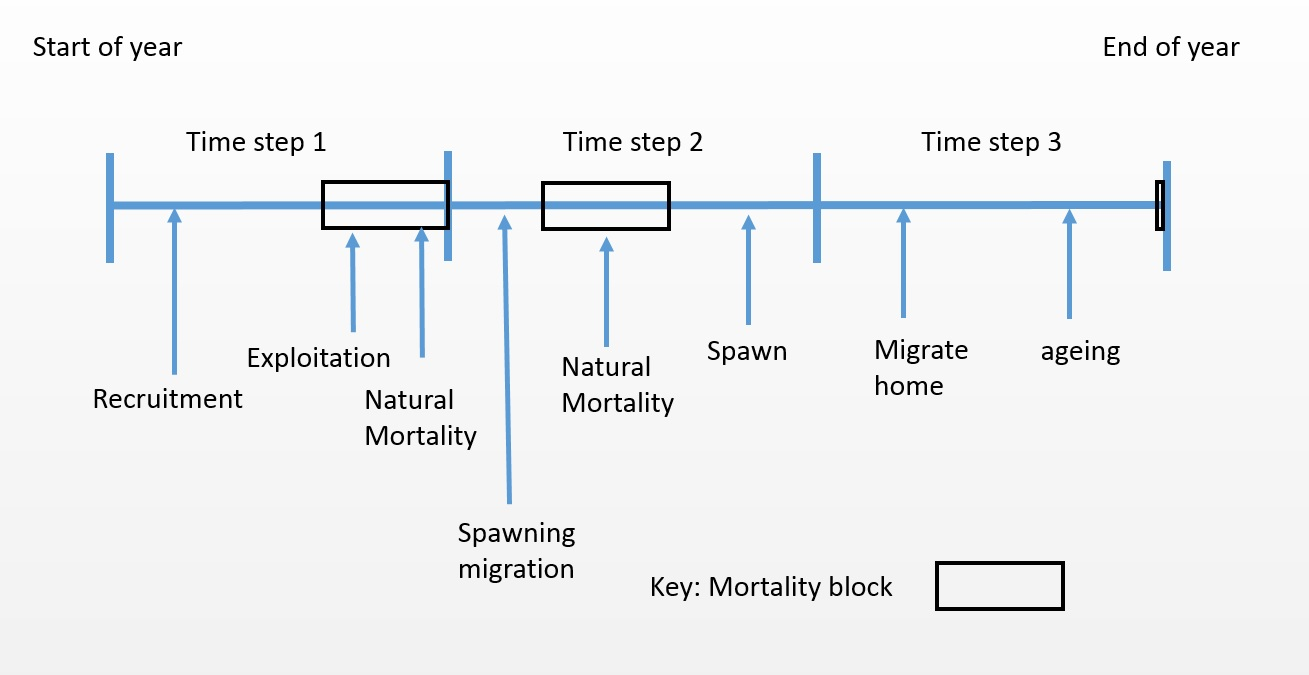
\includegraphics[scale=0.5]{Figures/annual_cycle.jpg}
	\caption{A example sequence for an annual cycle.}\label{Fig:annual}
\end{figure}

This would be specified using @time\_step block:

{\small{\begin{verbatim}
@model
time\_steps step1 step2 step3
\end{verbatim}}}

This gives the order and labels for each time step, i.e., 3. Processes are sequenced using order within the \textit{@time\_step} block:

{\small{\begin{verbatim}
@time_step step1
processes Recruitment Fishing

@time_step step2
processes Spawn_migration Fishing

@time_step step3
processes Home_migration Ageing
\end{verbatim}}}

The \emph{Recruitment}, \emph{Fishing}, \emph{Spawn\_migration}, \emph{Home\_migration} and \emph{Ageing} are all labels of command blocks that defines a process (see \ref{sec:Process} for the list of available processes). The order that the  processes are executed is in the same order as specified. The process \emph{Fishing} could be the process type \texttt{Instantaneous\_Mortality} (\ref{sec:Process-MortalityInstantaneous}) which takes natural mortality as a parameter as well as specifying the catches in the time-steps, so it is possible to have all catch taken in time-step \emph{step1} with some natural mortality, and no fishing in time-step \emph{step2} where the rest of the natural mortality occurs.

Although \emph{Spawn} represents a biological process, spawning, for the usual modelling it is the time that the spawning stock biomass is calculated since this is needed to calculate recruitment is there is a spawning biomass recruitment relationship. A related concept is maturity which can be in the partition, so there needs to be a transfer of immature fish into the mature category, i.e., a process, but it is only indirectly related to spawning. Hence, in modelling, spawning is not a process that affects the partition directly, but it the time to calculate the SSB which must be setup as a derived variable (from the partition). Hence, \emph{Spawn} is located in Figure \ref{Fig:annual}.

To calculate the SSB a \texttt{@derived\_quantity} command block is needed in which the "timing" of the SSB calculation in terms of which time-step and the proportion of natural mortality within it is specified (\ref{sec:DerivedQuantity}).

\subsubsection{\I{The initialisation phases}}\label{sec:Initialisation}

Initialisation is the process of determining the model starting state at the start of the first year (\texttt{Start\_year}. The initial state can be equilibrium/steady state or some other initial state for the model (e.g., exploited), prior to the start year of the model.

There are multiple options for partition initialisation in \CNAME, including

\begin{itemize}
	\item Iterative: run the model for a specified number of years to get the converged state.
	\item Derived: Use the analytical solution (i.e., faster than iterative) for the initial state, but it does not work for some processes (e.g., density dependant migration)
	\item Cinitial: Allow the estimation of the initial partition's numbers-at-age
	\item state\_category\_by\_age: specify the partition's numbers-at-age
\end{itemize}

Initialisation specifications starts with nominating the initialisation label in the \textit{@model} command block followed by a \textit{@initialisation\_phase} command block specifying the type and other settings:

{\small{\begin{verbatim}
@model
...     # other subcommands
initialisation_phase int_label

@initialisation_phase int_label
type iterative  #choose one from the list above
...             # specify option values

\end{verbatim}}}

If needed, the processes used and their order in the initialisation are those specified in the annual cycle, but these can by changed by either excluding some processes or including others by using the  \texttt{exclude\_processes} or  \texttt{insert\_processes} subcommands in the \textit{initialisation\_phase} command blocks,

{\small{\begin{verbatim}

@initialisation_phase int_label
type iterative
exclude_processes Fishing
insert_processes step1(recruitment)=initialFishing
            #format=<step>(<insert before label>)-<new block label>
...             # specify option values

\end{verbatim}}}

where \textit{ Fishing} is the normal fishing process which defines natural mortality so when excluded, initialisation can use another value that incorporates some unrecorded fishing before the start of the assessment period by setting natural mortality to a higher value in the process \textit{initialFishing}. The place to insert \textit{initialFishing}is in the time-step labelled \textit{step1} before the process \textit{recruitment} which must be in that time-step (process label is enclosed in brackets). To insert at the end of the time-step use \textit{()}, i.e. \textit{step1()=initialFishing}.

Normally,the type \textit{iteration} is used, but more complicated initialisation can by used by sequencing other phases one after another,

{\small{\begin{verbatim}
@model
...     # other subcommands
initialisation_phase int_label int_label2


@initialisation_phase int_label
type derived    #choose one from the list above
...             # specify option values

@initialisation_phase int_label2
type iterative    #choose one from the list above
...             # specify option values

\end{verbatim}}}

which may be faster overall since less iterations can be used in the second phase. The order of applying each initialisation is that given in the \textit{@model} command block.

The multi-phased initialisation allows for flexibility in the number and type of initialisation, for initialising a non-equilibrium starting state, or applying simple processes before applying more complex ones.

In each initialisation phase, the processes defined for that phase are applied and used as the starting point for the following phase or, if it is the last phase, the start year of the model.

The \emph{first} initialisation phase is always initialised with each age and category set to zero. Care must be taken when using complex category inter-relationships or density-dependent processes that depend on a previously calculated state, as they may fail when used in the first phase of an initialisation.

Multi-phase iterations\index{Multi-phase iteration} can also be used to determine if an initialisation has converged. A second initialisation phase can be added for 1 year, with the same processes applied as in the first phase. The state at the end of the first and second phase is then output. If these states are identical, then it is likely that the initialisation has converged to an equilibrium state.

\paragraph{\I{Iterative Initialisation}}\label{sec:InitialisationPhase-Iterative}

The \texttt{iterative} initialisation is a general solution for initialising the model, but can be slow to converge, depending on the model.Its value is that it can work on complex structured models that may be difficult or impossible to implement using analytic approximations.

The number of iterations in the iterative initialisation can increase the model output, and the number of iterations should be chosen to be large enough to allow the population state to fully converge. A period of about two times the maximum age is recommended to ensure convergence. \CNAME\ can be configured to report convergence statistics that can assist in determining convergence properties.

In addition, the iterative initialisation phase can optionally be stopped early if user-defined convergence criteria is met. For a list of supplied years in the initialisation phase, the convergence criteria is met if the proportional absolute summed difference between the state in year $t-1$ and the state in year $t$ ($\widehat{\lambda}$) is less than the user-defined value of $\lambda$, where

\begin{equation}
  \widehat{\lambda} = \frac{\sum\limits_{i,j}  \left|\text{element}(t)_{i,j} - \text{element}(t-1)_{i,j} \right|}{\sum\limits_{i,j} \frac{}{}\text{element}(t)_{i,j}}
\end{equation}

where $\text{element}(t)_{i,j}$ denotes the numbers at time step $t$ in category $j$ and age class $i$.

Hence, for the initialisation define:

\begin{itemize}
  \item The number of initialisation phases,
  \item The number of years in each phase, and
  \item The processes to apply in each phase, where the default processes are those applied in the annual cycle
\end{itemize}

An example with one initialisation phase:

{\small{\begin{verbatim}
@model
...
initialisation_phases Iterative_initialisation

@initialisation_phase Iterative_initialisation
type iterative
years 50                # do 50 iterations
lambda 0.0001
convergence_years 20 40 # test for convergence at 20 and 40 iterations
\end{verbatim}}}

\paragraph{\I{Derived Initialisation}}\label{sec:InitialisationPhase-Derived}

The \texttt{derived} initialisation is an analytical solution that calculates the equilibrium age structure and the plus group using a geometric series solution. The benefit of this method is it can be solved in \texttt{max\_age - min\_age + 1} years or time-steps units, so it is computationally faster than the iterative initialisation phase. Under some process combinations (e.g., one-way migrations) this initialisation does not calculate the exact equilibrium partition. When using this initialisation, confirm that the partition has reached an equilibrium state by either comparing with an iterative initialisation, or by adding a second iterative initialisation phase with a limited number of iterations for comparison.

An example with one initialisation phase:

{\small{\begin{verbatim}
		@model
		...
		initialisation_phases Equilibrium_initialisation

		@initialisation_phase Equilibrium_initialisation
		type derived
		\end{verbatim}}}


When a model is initialised with this method, and recruitment is defined by \(B_0\), the model initialises the partition with an \(R_0 = 1\). Once the initialisation phase is complete, it scales all the categories defined in each recruitment process by
\[
N_{a,c}  = N_{a,c} \times B_0^R / SSB^R  \ .
\]
where, \(R\) denotes each recruitment block and \(N_{a,c}\) are categories defined in that recruitment block. For this case, it is advised to associate all categories to the recruitment so they are accounted for in this scaling process. If maturity is in the partition, it is not intuitive to define mature categories with a proportion set = 0 in a recruitment process. However, this is exactly what is needed to scale the partition to the correct equilibrium state. \CNAME\ will flag a warning if a model doesn't have all categories defined in the available recruitment blocks. A case where this can be ignored is in models with tagged categories, these categories don't exist in initialisation and so don't need to be scaled, thus can be omitted from the recruitment definition. \CNAME\ will still output a warning for this, but can be ignored if users understand its purpose.

\paragraph{\I{Cinitial Initialisation}}\label{sec:InitialisationPhase-Cinitial} \STATUS{Untested}

The \texttt{cinitial} initialisation can only be applied after \textit{derived} or \textit{iterative} initialisation phases. This initialisation can be a method for estimating the non-equilibrium state of population if there is exploitation before data is collected. The estimated \textit{cinitial} factors shift the initial population away from an equilibrium state prior to the start year.

After the first initialisation phase we have an equilibrium age-structure denoted by $N_{equil}$.

\textit{Ciniital} specifies an age structure denoted by $N_{cinit}$ (in numbers), but this can be combinations of categories, say both sexes by two areas.

$Multiplier =  N_{cinit} / N_{equil}^{combined}$

where $N_{equil}^{combined} $ is summed over the same combined categories as \textit{Cinitial}. Then

$N_{init} =  N_{equil} * Multiplier $

$N_{init}$ is the numbers-at-age by category for the start of the model run.

It would be helpful to include an observation of age composition data for the first year of the model in order to estimate the non-equilibrium population state.

An example with two initialisation phases:

{\small{\begin{verbatim}
		@model
		...
		initialisation_phases Iterative Cinitial

		@initialisation_phase Iterative
		type iterative
		years 10
		lambda 0.0001
		convergence_years 10 20

		@initialisation_phase Cinitial
		type cinitial
		categories spawn.male+nonspawn.male spawn.female+nonspawn.female
		table n
		spawn.male+nonspawn.male     5e7 5e7 7e6 6e6 5e6 4e6 3e6 2e6 1e6 1e6 1e1 1e1 1e1 1e1
		spawn.female+nonspawn.female 5e7 5e7 7e6 6e6 5e6 4e6 3e6 2e6 1e6 1e6 1e1 1e1 1e1 1e1
		end_table
		\end{verbatim}}}

The Cinitial factors can also be estimated with the syntax

{\small{\begin{verbatim}
	@estimate cinit_male
	parameter initialisation_phase[Cinitial].spawn.male+nonspawn.male
	same initialisation_phase[Cinitial].spawn.female+nonspawn.female
	lower_bound  2e2  2e2  2e2  2e2  2e2  2e2  2e2  2e2  2e2  2e2  2e0  2e0  2e0  2e0
	upper_bound  2e9  2e9  2e9  2e9  2e9  2e9  2e9  2e9  2e9  2e9  2e9  2e9  2e9  2e9
	type uniform
	\end{verbatim}}}

\paragraph{\I{State\_category\_by\_age}}\label{sec:InitialisationPhase-StateCategoryByAge} \STATUS{Untested}

The \texttt{state\_category\_by\_age} initialisation uses a user-defined table as the initial partition numbers-at-age for the beginning of the  start year. Models can be initialised by specifying the numbers-at-age for each category.

An example with one initialisation phase:

{\small{\begin{verbatim}
		@model
		...
		initialisation_phases Fixed

		@initialisation_phase Fixed
		type state_category_by_age
		categories male female
		min_age 3
		max_age 10
		table n
		male   1000 900 800 700 600 500 400 700
		female 1000 900 800 700 600 500 400 700
		end_table
		\end{verbatim}}}

When initialising models with this type, undefined behaviour may result if the model applies processes that require derived quantities to be calculated in the initialisation phase. (e.g., SSB so that recruitment can be calculated for the start year). In the latter case, you would have to use a subsequent initialisation phase \textit{iterator} that has natural mortality set to zero (i.e., \textit{insert\_processes} subcommand to introduce zero natural mortality and \textit{exclude\_processes} to exclude the mortality process that defines natural mortality) for as many year needed to set up the SSBs.


\subsection{\I{Population processes}}\label{sec:Process}

Population processes are processes that change the model state. These processes produce changes in the partition by adding or removing individuals, or by moving individuals between ages and/or categories.

Current population processes available include:

\begin{itemize}
\item recruitment\index{Recruitment} (Section~\ref{sec:Process-Recruitment}),
\item ageing\index{Ageing} (Section~\ref{sec:Process-Ageing}),
\item growth\index{Growth} (Section~\ref{sec:AgeLength}),
\item maturation\index{Maturation} (Section~\ref{sec:Process-TransitionCategory}),
\item mortality\index{Mortality} events (e.g., natural and fishing) (Section~\ref{sec:Process-Mortality}), 
\item category transition processes\index{Category transition}, i.e., processes that move individuals between categories while preserving their overall age structure (Section~\ref{sec:Process-TransitionCategory}), and
\item tagging and tag loss (Section~\ref{sec:Process-TagByAge}).
\end{itemize}

There are two types of processes: (1) processes that occur across multiple time steps in the annual cycle, e.g., \subcommand{mortality\_constant\_rate} and \subcommand{mortality\_instantaneous}; and (2) processes that occur only within the time step in which they are specified.

\subsubsection{\I{Recruitment}}\label{sec:Process-Recruitment}

Recruitment processes  add new individuals to the partition. Recruitment depends on virgin biomass or alternatively recruitment in the virgin state and so these parameters are located in this process (as \textit{b0} and \textit{r0}). The other factors needed are SSB if there is a stock-recruitment relationship and the CV for the prior on YCS (the mean is mandated to be 1 over some specified year range). Thus, a SSB label may have to be included (pointing to a derived quantity).

In the recruitment processes, a number of individuals are added to a single age class (subcommand \textit{age}) within the partition, with the number determined by the type of stock-recruitment process specified. If recruits are added to more than one category, then the proportion of recruits to be added to each category is specified by the \argument{proportions} subcommand. For example, if recruiting to categories labelled \texttt{male} and \texttt{female}, then the proportions may be set to $0.5$ and $0.5$, so that half of the recruits are added to the male category and the other half to the female category.

Recruitment can differ between a spawning event or the creation of a cohort/year class. One view for fisheries is that recruitment usually refers to individuals "recruiting" to a fishery. This definition is used because there is usually not a lot of information on younger age classes between the time of spawning and being vulnerable to a survey or fishery for data collection. However, here, recruitment is to a fixed age class for one or more categories.

The offset between spawning and recruitment is parametrised either by the recruitment subcommand \texttt{age}, or \texttt{min\_age}, which is the default value for the \texttt{age} subcommand in the recruitment process. The \CNAME\ parameter \texttt{age} is the same as the CASAL parameter \texttt{y\_enter}.\TODO{Check this} Notice that the minimum age is usually different from zero and so there is usually  a one or more year's delay between spawning and recruitment into the partition. There is also a complication from when spawning occurs in the annual cycle and when recruitment occurs.

\CNAME\ has two  recruitment processes, constant recruitment\index{Recruitment ! Constant} and the \I{Beverton-Holt stock-recruitment relationship}\index{Recruitment ! Beverton-Holt} \citep{1203}. The  number of individuals following recruitment in year $y$ is

\begin{equation}
N_{y,a,j} \leftarrow N_{y,a - 1,j} + p_j(R_y)
\end{equation}

where $N_{y,a,j}$ is the numbers in year $y$ and category $j$ at age $a$, $p_j$ is the proportion added to category $j$, and $R_y$ is the total number of recruits in year $y$.

\paragraph{\I{Constant recruitment}}\label{sec:Process-RecruitmentConstant}

In the constant recruitment process the total number of recruits added in each year $y$ in age $a$ is $R_y$, with $R_y = R_0$ for all years

\begin{equation}
  R_{y,j} = p_j(R_0)
\end{equation}

Constant recruitment is equivalent to a Beverton-Holt recruitment process with steepness ($h$) set to 1.

For example, to specify a constant recruitment process where individuals are added to the male and female immature categories at $age=1$ in equal proportion (\texttt{proportions} = 0.5), and the number to add is $R_0=5 \times 10^5$, the syntax is

{\small{\begin{verbatim}
	@process Recruitment
	type constant_recruitment
	categories male.immature female.immature
	proportions 0.5 0.5
	r0 500000
	age 1
\end{verbatim}}}

\paragraph{\I{Beverton-Holt recruitment}}\label{sec:Process-RecruitmentBevertonHolt}

In the Beverton-Holt recruitment process the total number of recruits added each year is $R_y$. $R_y$ is the product of the average recruitment $R_0$, the annual year class strength multiplier $YCS$, and the stock-recruit relationship $SR(SSB_y)$

\begin{equation}\label{eq:BH}
  R_{y,a,j} = p_j(R_0 \times YCS_{ycs\_year} \times SR(SSB_{ycs\_year}))
\end{equation}

where

\begin{equation}\label{eq:year_class}
ycs\_year = y - \texttt{ssb\_offset}
\end{equation}

and $a$ is age, $p_j$ is the proportion of recruits to enter category $j$, and \texttt{ssb\_offset} is the number of years lag between spawning and recruitment.

Recruitment refers to recruitment into the population and may differ from the spawning event. See below on more information about \texttt{ssb\_offset}. In general this parameter should not be specified by the user.

$SR(SSB_y)$ is the Beverton-Holt stock-recruit relationship parametrised by the steepness $h$, and based on \cite{mace_doonan_88} parametrisation

\begin{equation}\label{eq:BH_SR}
SR(SSB_y) = \frac{SSB_y}{B_0} / \left( 1-\frac{5h-1}{4h} \left( 1-\frac{SSB_y}{B_0} \right) \right)
\end{equation}

The Beverton-Holt recruitment process requires a value for \Bzero\ and $SSB_y$ to calculate the number of recruits. A derived quantity (see Section \ref{sec:DerivedQuantity}) must be defined that provides the annual $SSB_y$ for the recruitment process. \Bzero\ is then defined as the value of the $SSB$ at the end of one of the initialisation phases, which is defined by the parameter \texttt{b0\_initialisation\_phase}.

During initialisation the $YCS$ multipliers are assumed to be equal to 1, and recruitment that happens in the initialisation phases that occur before and during the phase when \Bzero\ is determined are assumed to have steepness $h=1$ (i.e., in those initialisation phases, recruitment is equal to \Rzero).

Recruitment in the initialisation phases after the phase where \Bzero\ was determined are calculated using the Beverton-Holt stock-recruit relationship. \Rzero\ and \Bzero\ have a direct relationship when there are no density-dependent processes in the annual cycle. Models can thus be initialised using \Bzero\ or \Rzero.

An example of the specification of a Beverton-Holt recruitment process, where individuals are added to the category "immature" at $age=1$, and the number added is $R_0=5 \times 10^5$; \texttt{SSB\_derived\_quantity} is a derived quantity that specifies the total spawning stock biomass that contributed to the year class, with \Bzero\ the value of the derived quantity at the end of the initialisation phase labelled \texttt{phase1}; and $YCS$ are standardised to have mean one in the period 1995 to 2004, and recruits enter into the model two years following spawning

{\small{\begin{verbatim}
	@process Recruitment
	type recruitment_beverton_holt
	categories immature
	proportions 1.0
	r0 500000
	b0_initialisation_phase phase1
	steepness 0.75
	age 1
	ssb SSB_derived_quantity

\end{verbatim}}}

The property \texttt{ssb\_offset} should not be manually specified; \CNAME\ determines \texttt{ssb\_offset} by the order of ageing, recruitment, spawning, and the recruitment parameter \texttt{age}

\begin{itemize}
	\item if the annual time step order is recruitment, ageing, spawning, then \texttt{ssb\_offset} should equal \texttt{age} + 1, or
	\item if the annual time step order is spawning, ageing, recruitment, then \texttt{ssb\_offset} should equal \texttt{age} - 1, or
	\item \texttt{ssb\_offset} = \texttt{age}
\end{itemize}

There may be scenarios where the user will input these values, e.g., if there are multiple ageing processes in the annual cycle. \CNAME\ does not have functionality to accommodate this situation, so in this case \texttt{ssb\_offset} would be manually defined.

There are two variants of this process and they refer to how the stock recruitment residuals or $YCS_{ycs\_year}$ are parametrised. This parametrisation can either be in natural space as year class strength ($YCS$) multipliers, or in log space as recruitment deviations. Due to the difference in terminology, these variants are implemented in two separate processes, \subcommand{type recruitment\_beverton\_holt} and \subcommand{type recruitment\_beverton\_holt\_with\_deviations}, respectively.

\paragraph*{YCS ($YCS_y$)}

The $YCS$ parameter (\texttt{ycs\_years}) is defined in Equation~\eqref{eq:year_class}. The parameter \texttt{ycs\_values} is referenced by the \texttt{ycs\_years} parameter and is important to note when defining \command{estimate}, \command{project}, and \command{time\_varying} blocks for the parameter \texttt{ycs\_values}. An example is at the end of the section.

A common practice when estimating $YCS$ is to standardise using the Haist parametrisation, which was described by V. Haist. \CNAME\ will standardise $YCS$ only if subcommand \subcommand{standardise\_ycs\_years} is defined. The model parameter \texttt{ycs\_values} is a vector \textbf{Y}, covering the years from \texttt{start\_year} - \texttt{ssb\_offset} to \texttt{final\_year} - \texttt{ssb\_offset}, as defined by the parameter \texttt{ycs\_years}. The resulting year class strengths are calculated by $YCS_i=Y_i/\bar{\textbf{Y}}$, where the mean is calculated over the user-specified years \texttt{standardise\_ycs\_years}.

\[
YCS_i =
\begin{cases}
Y_i / mean_{y \in S}(Y_y) & :y \in S\\
Y_i					 & :y \notin S
\end{cases}
\]

where S is the set of years from \texttt{standardise\_ycs\_years}. One effect of this parametrisation is that \Rzero\ is then defined as the mean estimated recruitment over the set of years $S$, because the mean $YCS$ multiplier over these years will always be one.

Typically \texttt{standardise\_ycs\_years} is defined to span the years over which $YCS$ is reasonably well estimated. For years that are not well estimated, $Y_y$ can be set to 1 for some or all years $y\in S$ (which is equivalent to forcing $R_y$ = \Rzero\ x $SR(SSB_y)$) by setting the lower and upper bounds of these $Y$ values to 1. An exception to this might occur for the most recent $YCS$ values, which the user may estimate but not include in the definition of \Rzero\ (because the estimates may be based on too few data). One or more years may be excluded from the range of years for the averaging process of the Haist parametrisation.

The advantage of the Haist parametrisation is that a large penalty is not necessary to force the mean of the $YCS$ parameter to be 1, although a small penalty should still be used to stop the mean of \textbf{Y} from drifting. These adjustments may improve MCMC performance. Projected $YCS$ values are not affected by this feature. A disadvantage with this parametrisation in a Bayesian analysis is that the prior applies to $Y$, not $YCS$.

In the  example given above,  $YCS$ are standardised to have mean one in the period 1995 to 2004, and recruits enter into the model two years following spawning

{\small{\begin{verbatim}
	@process Recruitment
	type recruitment_beverton_holt
	...            #subcommand above
	standardise_ycs_years 1995:2004
	ycs_years  1994 1995 1996 1997 1998 1999 2000 2001 2002 2003 2004 2005 2006
	ycs_values 0.65 0.87  1.6 1.13 1.02 0.38 2.65 1.35    1    1    1    1    1
\end{verbatim}}}


\paragraph*{Recruitment deviations, $\epsilon_y$ (\emph{type recruitment\_beverton\_holt\_with\_deviations})} \label{sec:Process-RecruitmentBevertonHoltWithDeviations} \STATUS{Untested}

Recruitment deviations represent the stock-recruitment relationship residuals in log space, with the link between $YCS_y$ and $\epsilon_y$

\begin{equation}\label{eq:recruit_devs}
	YCS_y = exp(\epsilon_y - b_y\sigma^2_R / 2)
\end{equation}

where $\epsilon_y\sim N(0,\sigma^2_R)$, $\sigma^2_R$ is the variance of the stock-recruitment residuals, and $b_y$ is a bias correction defined by \cite{methot2011adjusting}

\begin{equation}\label{eq::bias}
b_y = \left\{\begin{array}{lr}
0, & \text{for }y\leq y_1^b\\
b_{max}(1 - \frac{y - y_1^b}{y_2^b - y_1^b}), & \text{for } y_1^b < y < y_2^b\\
b_{max}, & \text{for } y_2^b\leq y \leq y_3^b\\
b_{max}(1 - \frac{y_3^b - y}{y_4^b - y_3^b}), & \text{for }  y_3^b< y < y_4^b\\
0, & \text{for } y_4^b\leq y
\end{array}\right\}
\end{equation}

The $\epsilon_y$ values are normally distributed in log space and thus lognormal when back-transformed to the resulting stock-recruitment relationship $YCS_y$. Recent work has found that this transformation does not technically lead to the \textit{a priori} assumption that the resulting $YCS_y$ are lognormal. \TODO{See Appendix investigating-two-options-for-ycs-prior-distribution-formulations for more details.}

The ramp function described above for the bias correction has the additional subcommands controlling the ramp

\begin{itemize}
	\item $y_1^b = $ \subcommand{last\_year\_with\_no\_bias}
	\item $y_2^b = $ \subcommand{first\_year\_with\_bias}
	\item $y_3^b = $ \subcommand{last\_year\_with\_bias}
	\item $y_4^b = $ \subcommand{first\_recent\_year\_with\_no\_bias}
	\item $b_{max} = $ \subcommand{b\_max}
\end{itemize}

{\small{\begin{verbatim}
@process Recruitment
type recruitment_beverton_holt_with_deviations
categories immature
proportions 1.0
r0 500000
last_year_with_no_bias 1940
first_year_with_bias 1950
last_year_with_bias 2016
first_recent_year_with_no_bias 2018
b_max 0.85
b0_initialisation_phase phase1
steepness 0.75
age 1
ssb SSB_derived_quantity
deviation_years  1994-2006
deviation_values 0 -0.2 0.4 0 0 0 0 0 0 0 0 0 0
\end{verbatim}}}

\paragraph*{Recruitment when modelling two stocks (or species)}

To specify a Beverton-Holt recruitment for each stock, the information required is:

\begin{enumerate}
	\item $YCS$, starting from year (\texttt{start\_year} - \texttt{ssb\_offset}) and extending up to year (\texttt{final\_year} - \texttt{ssb\_offset})
	\item the value of \texttt{age} (which is \texttt{y\_enter} in CASAL)
	\item the steepness parameter \texttt{h}
	\item in a multi category model, the proportion of recruits for each category
	\item a label for the derived quantity
\end{enumerate}

When an \command{initialisation\_phase} (Section~\ref{sec:Initialisation}) type = \subcommand{derived} is specified and the recruitment is defined by \subcommand{b0}, then all categories must be specified in the \command{recruitment} block. Usually in a recruitment processes only the categories that receive recruits need to be defined. For example, a population has a spawning area that is different from the area where recruits enter the population. An area-specific model could then be specified which contains spawning categories and recruiting categories. The recruiting categories would be specified in the subcommand \subcommand{categories}, as these would be the categories receiving recruits.

If \command{initialisation\_phase}, \subcommand{type=derived} is used, then all categories that are a part of that recruitment process need to be specified as well. For example,

{\small{\begin{verbatim}
@process Recruitment_stock1
type recruitment_beverton_holt
categories stock1.immature.M stock1.immature.female stock1.spawn.male stock1.spawn.female
proportions 0.5 0.5 0.0 0.0
r0 500000
ssb SSB1
....
\end{verbatim}}}

{\small{\begin{verbatim}
@process Recruitment_stock2
type recruitment_beverton_holt
categories stock2.immature.male stock2.immature.female stock2.spawn.male stock2.spawn.female
proportions 0.5 0.5 0.0 0.0
r0 200000
ssb SSB2
....
\end{verbatim}}}

The \texttt{proportions = 0.0} for "spawn.male" and "spawn.female" are needed due to the way the derived initialisation phase works. The derived initialisation finds a solution for when \subcommand{r0} = 1.0 based on an infinite geometric series for the plus group, and scales the initial partition by \subcommand{r0}. Thus, if all categories are not specified, then those that are missed would not be initialised to true values and this could lead to inaccurate model outputs. This set-up extends to multiple-stock fisheries model configurations as well, where all of the categories that make up the stock need to be listed.

\subsubsection{\I{Ageing}\label{sec:Process-Ageing}}

The ageing process "ages" individuals, i.e., this process moves all individuals in the named categories $j$ from one age class $a$ to age class $a + 1$, or accumulates them if the last age class is a plus group.

The ageing process is defined as,
\begin{equation}
  \text{element}(a + 1,j) \leftarrow \text{element}(a,j)
\end{equation}

except in the case of the plus group (if defined),
\begin{equation}
  \text{element}(a_{\text{max}}, j) \leftarrow \text{element}(a_{\text{max}}, j) + \text{element}(a_{\text{max}-1}, j).
\end{equation}

For example, to apply ageing to the categories \texttt{immature} and \texttt{mature}, the syntax is

{\small{\begin{verbatim}
	@process Ageing
	type ageing
	categories immature mature
	\end{verbatim}}}

Note: the ageing process is \emph{NOT} applied by \CNAME\ by default --- it needs to be explicitly specified. As with all other processes, \CNAME\ will not apply a process unless it is defined and specified within the annual cycle. Hence, it is possible to specify a model where a category is not aged. \emph{\CNAME\ will not check or otherwise warn if there is a category defined where ageing is not applied.}

\subsubsection{\I{Mortality}\label{sec:Process-Mortality}}

There are 8 types of mortality processes available in \CNAME:

\begin{itemize}
	\item constant rate,
	\item event,
	\item biomass-event,
	\item instantaneous,
	\item instantaneous retained (discards),
	\item Holling,
	\item initialisation, and
	\item a density-dependent relationship based on prey suitability.
\end{itemize}

These processes remove individuals from the partition, either as a rate, as a total number (abundance), as a biomass of individuals or, as a combination of these. \CNAME\ does not (yet) implement the Baranov catch equation. However, instantaneous mortality is considered an approximation to the Baranov catch equation.

To apply both natural and biomass-event mortality, the mortality type \texttt{mortality\_instantaneous} can be specified. Or, you can use \texttt{mortality\_instantaneous\_retained}, where discards are allowed. Mortality blocks are special because they allow both natural mortality and fishing mortality at the same time. Note that all mortality processes occur within the mortality block of a time step. See Section~\ref{sec:MortalityBlock} for more information and definitions on mortality blocks.


\paragraph{\I{Timing evaluation interval; timing the point when observations are fitted or derived quantities are evaluated }}\label{sec:MortalityBlock}\label{sec:TimingEvaluationInterval}

\TODO{review; put into observations?}

Observations (see Section~\ref{sec:Observation})  and derived quantities (see Section~\ref{sec:DerivedQuantity}) need a concept called a \emph{timing evaluation interval} so that the "time" within a year can be specified for their fit or evaluation. This interval is intimately tied into mortality processes.

There can be one or more mortality processes specified within a time-step, but these must  be grouped sequentially, i.e., there cannot be a non-mortality process between any two mortality processes within any one time step. The sequence of mortality processes is called a \emph{timing evaluation interval}.  If no mortality processes occurs in a time step, then the \emph{timing evaluation interval} is defined to occur at the end of the time step, i.e., it is a virtual, unspecified,  process. Thus  each time step has one \emph{timing evaluation interval}.

\CNAME\ will output an error if more than one \textit{timing evaluation interval} occurs in a single time step.

The "time" for an observation or derived quantity is based on the proportion of mortality that has occurred within the \textit{timing evaluation interval}. The starting and ending partition are saved so that a partition can be estimated by  interpolation between the start and end partitions.

For example, the point of calculation can be set to a point  when 75 \% of the deaths from natural mortality plus catch has occurred The partition at this point is based on interpolating between the start and end of the interval as the partition is known at those points.  Two  methods are available: \texttt{weighted\_sum} and \texttt{weighted\_product}, and are defined as

\begin{itemize}
	\item \texttt{weighted\_sum}: after proportion $p$ through the mortality block, the partition elements are given by $n_{p,j} = (1 - p)n_j + p'_j$

	\item \texttt{weighted\_product}: after proportion $p$ through the mortality block, the partition elements are given by $n_{p,j} = n_j^{1-p} n'^p_j$
\end{itemize}

where $n_{p,j}$ is the derived quantity at proportion $p$ of the mortality block for category $j$, $n_j$ is the quantity at the beginning of the mortality block, and $n'_j$ is the quantity at the end of the mortality block.

In the case of a virtual \textit{timing evaluation interval}, the partition at the end of the time-step is used.

\TODO{REDO FIGURE TO REFLECT TEI rather than mortality blocks; have two mortality processes in step 2}

\begin{figure}[H]
	\centering
	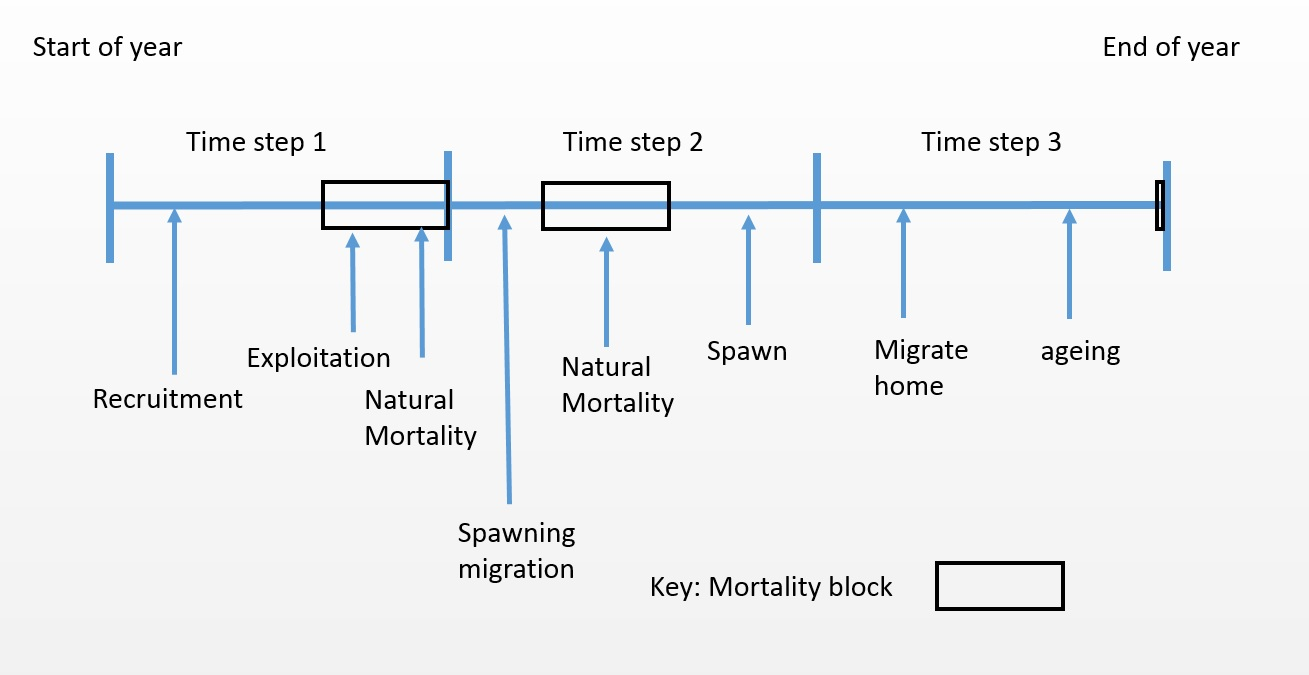
\includegraphics[scale=0.5]{Figures/annual_cycle.jpg}
	\caption{A example sequence for an annual cycle.}\label{Fig:annual2}
\end{figure}


\TODO{GO OVER M and specifying M-by-age HERE FOR ALL M-BASED PROCESSES}
\TODO{MAX U rate specification + Penalities}

\paragraph{Constant mortality rate}\label{sec:Process-MortalityConstantRate} \STATUS{Untested}

To specify a constant annual mortality rate \index{Constant mortality}(e.g. $M=0.2$) for categories "male" and "female"

{\small{\begin{verbatim}
# A process with label NaturalMortality
@process NaturalMortality
type          mortality_constant_rate
categories    male female
# effectively age related mortality
relative_m_by_age One One
m             0.2 0.2
\end{verbatim}}}

The total number of individuals removed from a category

\begin{equation}
D_{j,t} = \sum_a N_{a,j,t} [1 - \exp(-S_{a,j} M_{a,j} p_t)]
\end{equation}

where $D_{j,t}$ is the total number of deaths in category $j$ in time step $t$, $N_{a,j,t}$ is the number of individuals in category $j$ of age $a$ in time step $t$, $S_{a,j}$ is the selectivity value for age $a$ in category $j$, $M_{a,j}$ is the mortality rate for category $j$ for age $a$, and $p_t$ is the proportion of the mortality rate to apply in time step $t$.

The mortality rate process requires the specification of the mortality-by-age curve which is specified using a selectivity. To apply the same mortality rate over all age classes in a category, use a selectivity defined as $S_{a,j}=1.0$ for all ages $a$ in category $j$

{\small{\begin{verbatim}
@selectivity One
type constant
c 1
\end{verbatim}}}

Age-specific mortality rates can also be applied. For example, the hypothesis that mortality is higher for younger and older individuals and lowest when individuals are at their optimal fitness could be defined by using a double exponential selectivity (see Section~\ref{sec:Selectivity})

{\small{\begin{verbatim}
@selectivity age_specific_M
type double_exponential
x0 7.06524
x1 1
x2 17
y0 0.182154
y1 1.43768
y2 1.57169
alpha 1.0

@process      NaturalMortalityByAge
type          mortality_constant_rate
categories    male female
relative_m_by_age age_specific_M age_specific_M
m             1.0 1.0
\end{verbatim}}}

\TODO{INSERT FIG OF M-by-age}

In this definition \subcommand{m} is set to 1.0 and the rate is described through the selectivity. Otherwise, $M_{age} = S_{age} * m$. This concept can be constructed similarly for other mortality methods such as \subcommand{instantaneous\_mortality}.

\paragraph{Event and biomass-event mortality}\label{sec:Process-MortalityEvent}\label{sec:Process-MortalityEventBiomass} \STATUS{Untested?}

\TODO{WHEN NOT DOING M and FISHING AT THE SAME TIME}

The event mortality\index{Event mortality} and biomass-event mortality\index{Biomass-event mortality} processes are applied in a similar manner, except that they remove a specified abundance (number of individuals) or biomass, respectively. These mortality processes can be used to define mortality events where the numbers of removals are known, e.g., fishing, rather than applying mortality as a rate.

In these cases, the abundance or biomass removed is also constrained by a maximum exploitation rate. \CNAME\ removes as many individuals or as much biomass as possible,  while not exceeding the maximum exploitation rate.

Event mortality processes require a penalty to avoid estimating parameter values that will not allow the defined number of individuals to be removed. The model penalises those parameter estimates that result in an too low a number of individuals in the defined categories (after applying selectivities) to allow for removals at the maximum exploitation rate, with a similar penalty for biomass. See Section \ref{sec:Penalty} for more information on how to specify penalties.

The event mortality applied to user-defined categories $i$, with the numbers removed at age $j$ determined by a selectivity-at-age $S_j$:

First, calculate the vulnerable abundance for each category $j$ in $1 \ldots J$ for ages $a = 1 \ldots A$ that are subject to event mortality

\begin{equation}
  V_{a,j} = S_{a,j} N_{a,j}
\end{equation}

and define the total vulnerable abundance $V_{total}$ as

\begin{equation}
  V_{total}  = \sum\limits_j {\sum\limits_a {V_{a,j}}}
\end{equation}

The exploitation rate\index{Maximum exploitation rate} to apply is

\begin{equation}
U = \begin{cases}
  C/V_{total}, & \text{if $C/V_{total} \leq U_{max}$} \\
  U_{max}, & \text{otherwise}\\
  \end{cases}
\end{equation}

The number removed $R_{a,j}$ from each age $a$ in category $j$ is,

\begin{equation}
  R_{a,j} = U V_{a,j}
\end{equation}

For example, to specify an \textbf{abundance-based} fishing mortality process with catches given for a set of specific years over categories "immature" and "mature", with selectivity "FishingSel", and assuming a maximum possible exploitation rate of 0.7, the syntax is

{\small{\begin{verbatim}
	@process     Fishing
	type          event_mortality
	categories    immature mature
	years         2000 2001 2002 2003
	U_max         0.70
	selectivities FishingSel FishingSel
	penalty       event_mortality_penalty
	\end{verbatim}}}

and specified similarly for a \textbf{biomass-based} fishing mortality process

{\small{\begin{verbatim}
		@process      Fishing
		type          mortality_event_biomass
		categories    immature mature
		years         2000 2001 2002 2003
		U_max         0.70
		selectivities FishingSel FishingSel
		penalty      event_mortality_penalty
		\end{verbatim}}}

\paragraph{Instantaneous mortality}\label{sec:Process-MortalityInstantaneous}\label{sec:Process-MortalityInstantaneousEventBiomass}\label{sec:Process-MortalityInstantaneousEvent}

The instantaneous mortality process\index{Instantaneous mortality} combines both natural mortality and event biomass mortality into a single process. This allows the simultaneous application of both natural mortality and anthropogenic mortality to occur across multiple time steps. This process applies half the natural mortality in each time step, then the mortalities from all the concurrent removals instantaneously, then the remaining half of the natural mortality. In fisheries models this is the most commonly used mortality process

This process allows for multiple removal events, e.g., a fisheries model with multiple fisheries and/or fleets. A removal method can occur in one time step only, although multiple removals can be defined to cover events during the year.

The equations for instantaneous mortality:

\TODO{redo equations, as notation is not consistent with that above, e.g., $S_{a,j}$}

\begin{itemize}
	\item An exploitation rate (actually a proportion) is calculated for each fishery, as the catch divided by the selected-and-retained biomass,
	$$ U_f = \frac{C_f}{\sum_a \bar{w}_a S_{f,a} n_a exp(-0.5 t M_a)}$$
	\item The mortality pressure associated with method $f$ is defined as the maximum proportion of fish taken from any element of the partition in the area affected by the method $f$
	$$ U_{f,obs} = max_a(\sum_k S_{k,a} U_k) $$
	where the maximum is over all partition elements affected by fishery $f$, and the summation is over all methods $k$ which affect the $j$th partition element in the same time step as fishery $f$.

	In most cases the mortality pressure will be equal to the exploitation rate (i.e., $U_{f,obs} = U_f$), but can be different if: (a) there is another removal method operating in the same time step as removal method $f$ and affecting some of the same partition elements, and/or (b) the selectivity $S_{f,a}$ does not have a maximum value of 1.

	There is a maximum mortality pressure limit of $U_{f,max}$ for each method of removal $f$. So, no more than proportion $U_{f,max}$ can be taken from any element of the partition affected by removal method $f$ in that time step. Clearly, $0 \leq U_{max} \leq 1$. It is an error if two removal methods, which affect the same partition elements in the same time step, do not have the same $U_{max}$.

	For each $f$, if $U_{f,obs} > U_{f,max}$, then $U_f$ is multiplied by $U_{f,max}/U_{f,obs}$ and the mortality pressures are recalculated. In this case the catch actually taken from the population in the model will differ from the specified catch, $C_f$.

	\item The partition is updated using
		$$ n'_a = n_a exp(-tM_a)\big[1 - \sum_f S_{f,a} U_f \big] $$
\end{itemize}

For example, to apply natural mortality of $0.20$ across three time steps on both male and female categories, with two methods of removals (fisheries \texttt{FishingWest} and \texttt{FishingEast}) and their respective catches (kg) known for years 1975:1977 (the catches are given in the \texttt{catches} table and information on selectivities, penalties, and maximum exploitation rates are given in the \texttt{method} table), the syntax is

\TODO{where is \texttt{time\_step\_ratio} and its usage defined?}

{\small{\begin{verbatim}
	@process instant_mort
	type mortality_instantaneous
	m 0.20
	time_step_proportions 0.42 0.25 0.33
	relative_m_by_age One
	categories male female
	units kgs

	table catches
	year FishingWest FishingEast
	1975	80000	111000
	1976	152000	336000
	1977	74000	1214000
	end table

	table method
	method       category  selectivity u_max   time_step  penalty
	FishingWest   stock     westFSel    0.7     step1     CatchPenalty
	FishingEast   stock     eastFSel    0.7     step1     CatchPenalty
	end_table
	\end{verbatim}}}

and for referencing catch parameters for use in projecting, time-varying, and estimating, the syntax is

{\small{\begin{verbatim}
		parameter process[mortality_instantaneous].method_"method_label"{2018}
\end{verbatim}}}

where \subcommand{"method\_label"} is the label from the \subcommand{catch} or \subcommand{method} table and continuing the example,

{\small{\begin{verbatim}
		parameter process[instant_mort].method_FishingWest{2018}
\end{verbatim}}}

To calculate weight by empirical weight-at-age matrices as described in Section~\ref{sec:AgeWeight}, the method table would include an additional column to reference weight-at-age objects:

{\small{\begin{verbatim}
		@age_weight jan_weight_at_age
		type data
		table data
		year 1 		2 		3 		4
		1980 3.4	5.6		7.23 	8.123
		end_table

		table method
		method       category  selectivity  u_max  time_step  penalty       age_weight
		FishingWest  stock     westFSel     0.7    step1      CatchPenalty  jan_weight_at_age
		FishingEast  stock     eastFSel     0.7    step1      CatchPenalty  jan_weight_at_age
		end_table
\end{verbatim}}}


\paragraph{Instantaneous mortality with retained catch and discards}\label{sec:Process-MortalityInstantaneousRetained}

The instantaneous mortality retained process\index{Instantaneous mortality retained} builds on the instantaneous mortality process (\ref{sec:Process-MortalityInstantaneous}) which has simultaneous applications of fishing and natural mortality, but with all catch-at-sea being landed, i.e., no discarding. The process \texttt{mortality\_instantaneous\_retained} allows for retained catch, discards, and also a mortality to be applied to discards, i.e., some are allowed to survive. The method for taking catch from the partition and the constraints used are the same as in \texttt{mortality\_instantaneous}.

This process was implemented to address issues with the pot fishery for blue cod which has a minimum legal size and so some catch is discarded at sea and some of these discards are expected to survive (based on some experimental work). There are length data taken at sea, so the total catch selectivity can be estimated, and length and age data taken from the landed catch (retained), so the retention selectivity can also be estimated.

In this mortality process, discard mortality is specified by defining a selectivity to represent mortality by age or length (e.g., constant or asymptotic descending logistic).  This discard selectivity is not be estimated since there is no observation class associated with it. If discard mortality is not provided, it is assumed that all discards die. Landed catch, and both the retained and total catch selectivities must be specified.

Extending the example shown in instantaneous mortality process (\ref{sec:Process-MortalityInstantaneous}) to use retained weight instead of catch, the commands are:

{\small{\begin{verbatim}
@process FishingRetainedCatch
type mortality_instantaneous_retained
# natural mortality
m 0.20
# the ratio of natural mortality in each of the three time steps
time_step_proportions 0.42 0.25 0.33
relative_m_by_age One
#for natural mortality by age
categories male female
units kgs

table catches
# two fisheries, West and East
year FishingWest FishingEast
# the catches are now landed catch
1975 80000 111000
1976 152000 336000
1977 74000 1214000
end table

table method
# all discards die
method   category selectivity retained_selectivity u_max time_step      penalty
FishingWest stock    westFSel      westRetainedSel   0.7     step1 CatchPenalty
FishingEast stock    eastFSel      eastRetainedSel   0.7     step1 CatchPenalty
end_table
\end{verbatim}}}

If discard mortality is less than 1.0, use:

{\small{\begin{verbatim}
table method
# 50% discard mortality
method   category selectivity retained_selectivity discard_mortality u_max time_step penalty
FishingWest stock  westFSel    westRetainedSel         DisMort        0.7 step1 CatchPenalty
FishingEast stock  eastFSel    eastRetainedSel         DisMort        0.7 step1 CatchPenalty
end_table

@selectivity DisMort
Type constant
# 50% mortality of discards
c 0.5
\end{verbatim}}}

See the instantaneous mortality process (\ref{sec:Process-MortalityInstantaneous}) for referencing catch parameters and calculating weight using empirical weight-at-age matrices.

The report outputs total catch, actual landed catch, and discards, without and with discard mortality:

{\small{\begin{verbatim}
@report Mortality
type process
process Instantaneous_Mortality_Retained
\end{verbatim}}}

\TODO{redo notation, as it is not consistent with that above, e.g., $S_{a,j}$ and $R_y$}

In the following, fisheries are indexed by $f$, and $a$ indexes both age and category combinations.

The total catch is found by applying a selectivity, $S_{f,a}$, in the same way as in the instantaneous mortality process. Retention, $R_{f,a}$, is defined by specifying a selectivity, which can be a function of length or age. The retained catch is the product of these two values, $R_{f,a} * S_{f,a}$. If sex is in the partition, then there are potentially two retention curves, one for each sex.

In general, there is a retention curve for each category in the partition. This property does not apply to surveys. Discard mortality is also specified as a selectivity, $D_{f,a}$. The fraction of dead fish from fishing activity is $S_{f,a} * [ R_{f,a} + (1.0 - R_{f,a}) * D_{f,a} ]$. If $D_{f,a}$ is 1.0, then all selected fish are dead, and if it is 0.0, then only the retained fish are dead.

The equations for the \texttt{mortality\_instantaneous\_retained} process:

\begin{itemize}
    \item Total catch (catch-on-board), $C_{f}$, is calculated by (retained catch) * VF / VR, where VF is vulnerable retained biomass, $j$ indexes categories and $t$ is the proportion of M in the time step, and VF is the full vulnerable biomass, $VF = \sum_{a,j} \overline{w}_{a} S_{a,j} n_{a,j} \exp(-0.5 t M_{a,j})$.

    \item An exploitation rate (actually a proportion) is calculated for each fishery, as the total catch (retained + discards) divided by the selected biomass (VF above) using selectivity $S_{f,a}$,
        $$ U_f = \frac{C_f}{\sum_a \bar{w}_a S_{f,a} n_a \exp(-0.5 t M_{a})}$$

    \item The mortality pressure associated with method $f$ is defined as the maximum proportion of fish taken from any element of the partition in the area affected by the method $f$,
        $$ U_{f,obs} = max_a (\sum_k S_{k,a} U_k) $$
    where the maximum is over all partition elements affected by fishery $f$, and the summation is over all methods $k$ which affect the $j$th partition element in the same time step as fishery $f$.

    In most cases the mortality pressure will be equal to the exploitation rate (i.e., $U_{f,obs} = U_f$), but can be different if: (a) there is another removal method operating in the same time step as removal method $f$ and affecting some of the same partition elements, and/or (b) the selectivity $S_{f,a}$ does not have a maximum value of 1.

    There is a maximum mortality pressure limit of $U_{f,max}$ for each method of removal $f$. So, no more than proportion $U_{f,max}$ can be taken from any element of the partition affected by removal method $f$ in that time step. Clearly, $0 \leq U_{max} \leq 1$. It is an error if two removal methods, which affect the same partition elements in the same time step, do not have the same $U_max$.

    For each $f$, if $U_{f,obs} > U_{f,max}$, then $U_f$ is multiplied by $U_{f,max}/U_{f,obs}$ and the mortality pressures are recalculated. In this case the catch actually taken from the population in the model will differ from the specified catch, $C_f$.

    \item Discard numbers-at-age (including their share of natural mortality) is $S_{a,j} (1 - R_{a,j}) n_{a,j} \exp(-0.5 t M_{a,j})$, and those that die at the end of the time step (updating the partition) are $D_{a,j} S_{a,j} (1 - R_{a,j}) n_{a,j} \exp(-t M_{a,j})$, where $D_{f,a}$ is the fraction that die on return to the sea.

    \item The partition is updated by removing landed catch, natural mortality, and discard mortality
        $$ n'_{a} = n_{a} \exp(-t M_a) \big[ 1 - \sum_f S_{f,a} U_f (R_{f,a} + D_{f,a} (1 - R_{f,a})) \big] $$
\end{itemize}

\paragraph{\I{Holling mortality rate}}\label{sec:Process-MortalityHollingRate} \STATUS{Untested}

The density-dependent Holling mortality process\index{Holling mortality} applies the Holling Type II or Type III functions \citep{Holling1959}, and is generalised by the Michaelis-Menten equation \citep{MentenMichaelis1913}.

This mortality process removes a number or biomass from a set of categories according to the total (selected) abundance (or biomass) and some "predator" abundance (or biomass), and is constrained by a maximum exploitation rate.

The mortality applied to user-defined categories $k$, with the numbers removed at age $l$, determined by a selectivity-at-age $S_l$ is applied as follows:

First, calculate the total predator abundance (or biomass) over all predator categories $k$ in $1 \ldots K$ and ages $l = 1 \ldots L$ that are applying the mortality

\begin{equation}
	P_{k,l} = S^{predator}_l N^{predator}_{k,l}
\end{equation}

And define the total predator abundance (or biomass) $P_{total}$ as

\begin{equation}
	P_{total}  = \sum\limits_K {\sum\limits_L {P_{k,l}}}
\end{equation}

Then calculate the total vulnerable abundance (or biomass) over all prey categories $k$ in $1 \ldots K$ and ages $l = 1 \ldots L$ that are subject to the mortality

\begin{equation}
	V_{k,l} = S^{prey}_l N^{prey}_{k,l}
\end{equation}

Then define the total vulnerable abundance (or biomass) $V_{total}$ as

\begin{equation}
	V_{total}  = \sum\limits_K {\sum\limits_L {V_{k,l}}}
\end{equation}

The number to remove is then determined by

\begin{equation}
	R_{total} = P_{total} \frac{a  V_{total}^{x-1}}{b + V_{total}^{x-1}}
\end{equation}

where $x=2$ for the Holling type II function, $x=3$ for the Holling type III function, or a different value of $x \geq 1$ for the generalised Michaelis-Menten function; $a > 0$ and $b > 0$ are the Holling function parameters.

The exploitation rate\index{Maximum exploitation rate} to apply is

\begin{equation}
	U = \begin{cases}
		R_{total}/V_{total}, & \text{if $R_{total}/V_{total} \leq U_{max}$} \\
		U_{max}, & \text{otherwise}\\
	\end{cases}
\end{equation}

And the number removed $R$ from each age $l$ in category $k$ is

\begin{equation}
	R_{k,l} = U V_{k,l}
\end{equation}

The density-dependent Holling mortality process is applied either as a function of biomass or abundance, depending on the value of the \texttt{is\_abundance} switch.

For example, a biomass Holling type II mortality process on prey \texttt{prey} by predator \texttt{predator} has the syntax

{\small{\begin{verbatim}
		@process HollingMortality
		type Holling_mortality_rate
		is_abundance F
		a 0.08
		b 10000
		x 2
		categories prey
		selectivities One
		predator_categories predator
		predator_selectivities One
		u_max 0.8
\end{verbatim}}}

\paragraph{Initialisation-event mortality}\label{sec:Process-MortalityInitialisationEvent}\label{sec:Process-MortalityInitialisationEventBiomass} \STATUS{Untested}

Initialisation event mortality\index{Initialisation event mortality} is a process that can occur only in the initialisation phase. It applies abundance or biomass mortality events specifically in initialisation phases. This option can be useful if the population is not in equilibrium before model start.

This process applies a single catch value for all iterations within the initialisation phase, and mortality will not be applied outside of the initialisation phase. This process should not be embedded in the annual cycle.

This process should be used in conjunction with the \texttt{insert\_processes} command in the \command{initialisation\_phase} block.

Example syntax where the \texttt{initialisation\_mortality\_event} has been specified in the initialisation phase \texttt{Predation\_state} but not in the annual cycle:

{\small{\begin{verbatim}
initialisation_phases Equilibrium_state Predation_state
time_steps Oct_Nov Dec_Mar

@initialisation_phase Equilibrium_state
type derived

@initialisation_phase Predation_state
type iterative
insert_processes Oct_Nov()=predation_Initialisation

@process predation_Initialisation
type initialisation_mortality_event
categories male.HOKI female.HOKI
catch 90000
selectivities Hakesl Hakesl

time_step Oct_Nov
processes Mg1 Instantaneous_Mortality

@time_step Dec_Mar
processes Recruitment Instantaneous_Mortality
\end{verbatim}}}

\paragraph{Prey-suitability mortality}\label{sec:Process-MortalityPreySuitability} \STATUS{Untested}

The density-dependent prey-suitability mortality process\index{Density-dependent prey-suitability} applies predation mortality from a predator group to its prey groups simultaneously. It removes an abundance (or biomass) from each prey group according to the total (selected) abundance (or biomass) of each prey group, the total (selected) abundance (or biomass) of the other prey groups, some "predator" abundance (or biomass), and the preference (electivity) of the predator for each prey group, constrained by a maximum exploitation rate. The predator-prey suitability functions were based on the multispecies Virtual Population Analysis (MSVPA) functions \citep{JuradoMolina2005}.

The mortality applied to the user-defined prey group $g$ of category $k$, with the numbers removed at age $l$ determined by a selectivity-at-age $S_l$ is applied as follows:

First, calculate the total predator abundance (or biomass) over all predator categories $k$ in $1 \ldots K$ and ages $l = 1 \ldots L$ that are applying the mortality

\begin{equation}
P_{k,l} = S^{predator}_l N^{predator}_{k,l}
\end{equation}

And define the total predator abundance (or biomass) $P_{total}$ as

\begin{equation}
P_{total}  = \sum\limits_K {\sum\limits_L {P_{k,l}}}
\end{equation}

Then, given the total vulnerable abundance (or biomass) of prey group $g$ over all categories $k$ in $1 \ldots K$ and ages $l = 1 \ldots L$ that are subject to the mortality

\begin{equation}
V_{g,k,l} = S^{prey}_l N^{prey}_{k,l}
\end{equation}

And define the total vulnerable abundance (or biomass) of each prey group $V^g_{total}$ as

\begin{equation}
V^g_{total}  = \sum\limits_K {\sum\limits_L {V_{g,k,l}}}
\end{equation}

And the total availability $A^g_{total}$ for each prey group as

\begin{equation}
A^g_{total} = \frac{V^g_{total}}{\sum\limits_G {V^g_{total}}}
\end{equation}

The vulnerable abundance (or biomass) and availability every prey group $g$ in $1 \ldots G$ is calculated simultaneously. Then the abundance (or biomass) to remove from each prey group $g$ is a function of its electivity $E_g$, the availability of all other prey groups $i$ in $1 \ldots G$, the electivity of the predator for each prey group $E_i$, and the total consumption rate of the predator $CR$ and its abundance (or biomass) $P_{total}$

\begin{equation}
R^g_{total}=P_{total} CR \frac{A^g_{total} E_g}{\sum\limits_G {A^i_{total} E_i}}
\end{equation}

The exploitation rate\index{Maximum exploitation rate} to apply to each prey group $g$ is then

\begin{equation}
U_g = \begin{cases}
R^g_{total}/V^g_{total}, & \text{if $R^g_{total}/V^g_{total} \leq U_{max}$} \\
U_{max}, & \text{otherwise}\\
\end{cases}
\end{equation}

And the number removed $R^g$ in each prey group $g$ from each age $l$ in category $k$ is

\begin{equation}
R_{g,k,l} = U_g V_{g,k,l}
\end{equation}

Prey suitability choice occurs only between the prey groups specified by the process. The total predator consumption rate represents the consumption of the predator on those prey groups alone. The electivities must sum to 1. Further, the consumption rate can be modified by a layer to be cell specific.

The density-dependent prey-suitability process is applied as either a biomass or an abundance depending on the value of the \subcommand{is\_abundance} switch.

Individual categories can be aggregated into prey groups using the "+" symbol. To indicate that two (or more) categories are to be aggregated, separate them with a "+" symbol.

For example, to specify two prey groups of two species made up of the males and females in each prey group

{\small{\begin{verbatim}
		prey_categories maleSpeciesA + femaleSpeciesA maleSpeciesB + femaleSpeciesB
\end{verbatim}}}

This syntax indicates that there are two prey groups, \texttt{maleSpeciesA + femaleSpeciesA} and \texttt{maleSpeciesB + femaleSpeciesB}, with each group having its own electivity.

For example, a biomass prey-suitability mortality process with an overall consumption rate of $0.8$ of prey \texttt{species A} and \texttt{species B} (modelled as males and females) by the predator \texttt{predatorSpecies} with electivities between \texttt{species A} and \texttt{species B} of $0.18$ and $0.82$ has syntax

{\small{\begin{verbatim}
		@process PreySuitabilityMortality
		type prey-suitability_predation
		is_abundance F
		consumption_rate 0.8
		categories maleSpeciesA + femaleSpeciesA maleSpeciesB + femaleSpeciesB
		electivities 0.18 0.82
		selectivities One One One One
		predator_categories predatorSpecies
		predator_selectivities One
		u_max 0.8
\end{verbatim}}}

\subsubsection{\I{Transition By Category}}\label{sec:Process-TransitionCategory}

The transition by category process moves individuals between categories. This process is used to specify transitions such as maturation (individuals move from an immature to mature state) and migration (individuals move from one area to another).

There is a one-to-one relationship between the "from" category and the "to" category, i.e., for every source category there is one target category only

\begin{equation}
	N_{a,j} = N_{a,i} \times P_i \times S_{a,i}
\end{equation}

where $N_{a,j}$ is the number of individuals that have moved to category $j$ from category $i$ in age $a$, $N_{a,i}$ is the number of individuals in category $i$, $P_i$ is the proportion parameter for category $i$, and $S_{a,i}$ is the selectivity at age $a$ for category $i$.

To merge categories repeat the "to" category multiple times.

For example, to specify a simple spawning migration of mature males from a western area to an eastern (spawning) area, the syntax is

{\small{\begin{verbatim}
		@process Spawning_migration
		type transition_category
		from West.males
		to East.males
		selectivities MatureSel
		proportions 1
		\end{verbatim}}}

where \texttt{MatureSel} is a selectivity that describes the proportion of age or length classes that are mature and thus move to the eastern area.

\paragraph{Transition by category by age}\label{sec:Process-TransitionCategoryByAge}

A special process type is the transition by category by age process, which allows a transition to occur for a specific subset of ages in specific years only, where each year can have a different number that are moved between categories.

\subsubsection{\I{Tag Release events}}\label{sec:Process-TagByAge}\label{sec:Process-TagByLength} \STATUS{Untested}

Tagging processes can be age- or length-based processes, whereby numbers of individuals are moved from an untagged category to a tagged category defined in the \command{categories} block. Tag release processes can also account for initial tag-induced mortality on individuals.

Age-based tag release events move a known number of individuals tagged for each age to a tagged category, along with applying additional mortality. Individuals are removed from the non-tagged categories and added to tagged categories. Often the ages of tagged individuals are not known, so length-based tag release events are more commonly used.

Length-based tag release processes are more complicated, as the age-length matrix is calculated and the exploitation for each length bin to then move the correct numbers-at-age based on the known lengths of release. \CNAME\ also allows for initial tag loss.


\paragraph*{{Tag Release By Length}}
\subcommand{compatability\_switch casal2}\\

For each length bin $l$ of the input vector of numbers-at-length ${N}_l$, the vulnerable numbers at length for category \(j\) are calculated as

Create a new age-length 

$$\widetilde{T}_{a,l,j} = \phi_{a,l,j} S_{a,j}$$

$$ \widetilde{N}_{a,l,j}= \frac{\widetilde{T}_{a,l,j}}{\sum_a\sum_j \widetilde{T}_{a,l,j}} \times {N}_l$$

$$ \widetilde{N}_{a,j} = \sum_l \widetilde{N}_{a,l,j} $$

$$ u_{a,j} = \frac{\widetilde{N}_{a,j}}{N_{a,j} }  $$

$$
u_{a,j} =
\begin{cases}
u_{max},& \text{if } u_{a,j} > u_{max} \text{ \textbf{flag a penalty}}\\
u_{l},  & \text{otherwise}
\end{cases}
$$


$$
\widetilde{N}_{a,j} = N_{a,j} u_{a,j}
$$

Release mortality denoted by \(h_a\) can be applied before the process finished,

$$\widetilde{N_{a,j}} = \widetilde{N_{a,j}}\left(1.0 - h_a\right)$$


The syntax for an example of tag release by length process

{\small{\begin{verbatim}
@process 2005Tags_shelf
type tag_by_length
years 2005
from male.untagged+female.untagged
to male.2005  female.2005
selectivities ShelfselMale ShelfselFemale
penalty tagging_penalty
initial_mortality 0.1
table proportions
year 30 40 50 60 70 80 90 100 110 120 130 140 150 160 170 180 190 200 210 220
2005  0 0 0.0580 0.1546 0.3380 0.1981 0.1643 0.0531 0.0242 0.0097 0 0 0 0 0 0 0 0 0 0
end_table
n 207
U_max 0.999
\end{verbatim}}}

This process moves 207 individuals from a combination of male.untagged and female.untagged categories, based on the combination of growth rates and selectivity, into tagged male and tagged female categories.


For \subcommand{compatability\_switch casal}
This describes the algoirthm applied in CASAL, it should yield identical results when a single untagged category and tagged category are supplied. There is a small difference when input numbers at length are defined for a combination of categories (unsexed) and we allocated into each corresponding category (male and female). This is supplied for backwards compatibility with CASAL, we recommend using \subcommand{compatability\_switch casal2}. 


Given the input vector of proportions-at-length denoted by $\widetilde{p_l}$ and number of releases \(\widetilde{N}\), CASAL first calculates vulnerable numbers at age and length for all combined categories,

$$N_{a,l} = \sum_{j = 1} \phi_{a,l,j} N_{a,l,j} * S_a$$

Then it converts $\widetilde{p_l}$ to an age proportion denoted by  $\widetilde{p_a}$

$$\widetilde{p_a} = \widetilde{p_a} + \sum_{l = 1} \widetilde{p_l} \frac{N_{a,l}}{\sum_a N_{a,l}}$$
This assumption is thought to be less than ideal, because it ignores the length ratios between categories. $\widetilde{N_a}$ denotes the number of tags to release. 

$$\widetilde{N_a} = \widetilde{p_a} \widetilde{N}$$
At this point if \(\widetilde{N_a} > \sum_a N_{a,l}\) a penalty is flagged on the difference on these numbers at this point.

The tagged fish released for category \(c\)
$$\widetilde{N_{a,j}} = \widetilde{N_a} \frac{N_{a,l,c} }{\sum_a N_{a,l} }$$
%
Release mortality denoted by \(U_a\)  is applied as an exploitation proportion before the process finished,

$$\widetilde{N_{a,j}} = \widetilde{N_{a,j}} - \widetilde{N_{a,j}}\left(1.0 - U_a\right)$$

\subsubsection{\I{Tag loss}}\label{sec:Process-TagLoss} 
Tag Loss is the process which accounts for tagged fish being removed from the partition. For example tag related mortality or tag failure. This process is applied as an instantaneous mortality rate that can happen over multiple time steps in the annual cycle. This method assumes that when tags are lost the individuals are deleted from the model.


Two options are available depending on whether the tag release event were tagged with a single tag (\subcommand{tag\_type single}) and double tag (\subcommand{tag\_type double}).

For elements in the partition indexed by age \(a\) and category \(c\) , the number of tag lost (\(N^*_{c,a}\)) at time step \(t\) with loss rate \(r\) and proportion denoted by \(p^t\) for type \subcommand{single} is
\begin{equation}
	N^*_{c,a} = N_{c,a} exp\left( - r_a p^t\right)
\end{equation}
%
where \(N_{c,a}\) is the number of tagged fish before the process is applied.

For tag type \subcommand{double}
\begin{equation}
N^*_{c,a} = 1 - \left(1 - N_{c,a} exp\left( - r_a p^t\right)\right)\left(1 - N_{c,a} exp\left( - r_a p^t\right)\right)
\end{equation}
%


The syntax for the tag loss process follows
{\small{\begin{verbatim}
@process Tag_loss
type tag_loss
categories single_tagged_fish
tag_loss_rate 0.02
time_step_proportions 0.25 0.75
selectivities One
tag_loss_type single
year 1985
\end{verbatim}}}
and double tagged

{\small{\begin{verbatim}
	@process Tag_loss
	type tag_loss
	categories double_tagged_fish
	tag_loss_rate 0.02
	time_step_proportions 0.25 0.75
	selectivities One
	tag_loss_type double
	year 1985
\end{verbatim}}}
\subsection{\I{Derived quantities}\label{sec:DerivedQuantity}}

Some processes require a population value derived from the population state as an argument. These values are \texttt{derived quantities}. Derived quantities are values calculated in a specified time step in every year, and thus have a single value for each year of the model. The time within the time-step is at the end unless otherwise specified (using \textit{proportion\_mortality}-like subcommand.

Derived quantities can be calculated as either abundance or biomass. Abundance-derived quantities are the sum over the specified categories (after applying a selectivity)\label{sec:DerivedQuantity-Abundance}. Biomass-derived quantities are calculated similarly\label{sec:DerivedQuantity-Biomass}.

Derived quantities are also calculated during the initialisation phases. Therefore, the time step during each initialisation phase must be specified. If the initialisation time steps are not specified, the derived quantity will be calculated during the initialisation phases. \TODO{review}

A common use of an derived quantities is as input into a stock-recruit relationship  which requires an equilibrium biomass ($B_0$) and annual spawning stock biomass values ($SSB_y$) to calculate recruitment into the first age class. $SSB_y$ is an derived quantity based on the mature biomass, usually at spawning time.

Derived quantities can be associated with a \textit{time evaluation interval}; see section~\ref{sec:MortalityBlock} for more detail on mortality blocks. In this case, the point of calculation can be set to any point within the mortality block, e.g., when 75 \% of the deaths from natural mortality plus catch has occurred, which is based on interpolating between the start and end of the block as the partition is known at those points.  Two  methods are available: \texttt{weighted\_sum} and \texttt{weighted\_product}, and are defined as

\begin{itemize}
	\item \texttt{weighted\_sum}: after proportion $p$ through the mortality block, the partition elements are given by $n_{p,j} = (1 - p)n_j + p'_j$

	\item \texttt{weighted\_product}: after proportion $p$ through the mortality block, the partition elements are given by $n_{p,j} = n_j^{1-p} n'^p_j$
\end{itemize}

where $n_{p,j}$ is the derived quantity at proportion $p$ of the mortality block for category $j$, $n_j$ is the quantity at the beginning of the mortality block, and $n'_j$ is the quantity at the end of the mortality block.

For example, to define a biomass-derived quantity spawning stock biomass, $SSB$, calculated at the end of the first time step (labelled \texttt{step\_one}), over all "mature" male and female categories and halfway through the mortality block using the \texttt{weighted\_sum} method, the syntax is

{\small{\begin{verbatim}
@derived_quantity SSB
type          biomass
time_step     step_one
categories    mature.male mature.female
selectivities One
time_step_proportion        0.5
time_step_proportion_method weighted_sum
\end{verbatim}}}

\subsection{\I{Age-length relationship}\label{sec:AgeLength}}

The age-length relationship defines the functional form of the length-at-age (and the weight-at-length; see Section \ref{sec:MeanWeight}) of individuals at age/category within the model.

There are four length-age relationship options. The first is the naive "no relationship", where each individual has length 1 regardless of age. The others are:  von Bertalanffy relationship, the Schnute relationship, and "data" (mean length-at-age for each model year).

The length-at-age relationship is used to calculate the length frequency given age, and with the length-weight relationship, the weight-at-age of individuals within an age/category. When defining length-at-age, the length-weight relationship must also be defined (see Section \ref{sec:MeanWeight}).


For most weight based processes, derived quantities and observations the users have the option of supplying a matrix of mean weight at age for each year see section~\ref{sec:AgeWeight}. If these are supplied then this age-length-weight process is ignored.


Changes in length-at-age during the year, i.e., growth between birthdays, are represented by incrementing age as specified by the \subcommand{time\_step\_proportions} parameter.
	
\subsubsection{The `none' relationship}\index{Age-length relationshsip!None}\label{sec:AgeLength-None}

The length of each individual is 1 for all ages, and the \texttt{none} length-weight relationship must also be used.

\subsubsection{The von Bertalanffy relationship}\index{Age-length relationshsip!von Bertalanffy}\label{sec:AgeLength-VonBertalanffy}

\begin{equation}
\bar{s}(age)= L_\infty \left( 1 - \exp \left( -k \left(age-t_0 \right) \right) \right)
\end{equation}

\subsubsection{The Schnute relationship}\index{Schnute}\label{sec:AgeLength-Schnute}

\begin{equation}
\bar{s}(age)=\displaystyle\begin{cases}
  \left[ y_1^b + (y_2^b - y_1^b) \dfrac{1-\exp \left(-a(age - \tau_1) \right)}{1-\exp \left(-a(\tau_2 - \tau_1) \right)} \right]^{1/b}, & \text{if $a\ne0$ and $b\ne0$} \\
  \AddVspace
  y_1 \exp \left[ \ln \left( y_2 / y_1 \right) \dfrac{1-\exp \left(-a(age - \tau_1) \right)}{1-\exp \left(-a(\tau_2 - \tau_1) \right)} \right], & \text{if $a\ne0$ and $b=0$} \\
  \AddVspace
  \left[ y_1^b + \left( y_2^b - y_1^b \right) \dfrac{age-\tau_1}{\tau_2 - \tau_1} \right]^{1/b}, & \text{if $a=0$ and $b\ne0$} \\
  \AddVspace
  y_1 \exp \left[ \ln \left( y_2/y_1 \right) \dfrac{age-\tau_1}{\tau_2 - \tau_1} \right] , & \text{if $a=0$ and $b=0$} \\
  \end{cases}
\end{equation}

The von Bertalanffy relationship has parameters $L_\infty$, $k$, and $t_0$. The Schnute relationship \citep{836} has parameters $y_1$ and $y_2$, which are the mean lengths at reference ages $\tau_1$ and $\tau_2$, and $a$ and $b$; when $b=1$, this relationship reduces to the von Bertalanffy relationship with $k=a$.

\subsubsection{Data: matrix of size at age relationship}\index{Age-length relationship!Data}\label{sec:AgeLength-Data}

There is an option to input empirical length at age by year, which is an alternative to using an age-length growth model such as the von Bertalanffy and Schnute model. \CNAME\ will interpolate values for missing years across time steps. The calculations of length-at-age throughout the model years occur in the same time step.

{\small{\begin{verbatim}
@age_length   male_AL
type          data
time_step_proportions 0.0 0.0   #use age at start of time-step
length_weight wgt_male          # needed to convert numbers-at-age into catch
distribution  normal            # distribution of lengths around the mean length
cv_first      0.1               # cv of the distribution at the first age
cv_last       0.1               # cv of the distribution at the maximum age
time_step_measurements_were_made step2
internal_gaps mean
external_gaps mean
table data # first line has column labels for year and then all the model ages
year     2     3     4     5     6    7     8      9    10    11    12
1980 30.13 34.90 38.43 40.61 42.45 43.02 43.94 43.63 43.36 43.70 43.84
1981 30.33 34.78 38.03 40.15 42.22 42.89 44.21 44.07 43.99 44.32 44.64
end_table
\end{verbatim}}}

When the values for \textit{cv\_last} and \textit{cv\_first} are different, the cv used for intermediate ages is, by default, interpolate by that age's mean length. There is a legacy switch for testing the conversion of models from CASAL into \CNAME, i.e., use the subcommand, \textit{by\_length false} which allows the interpolation to be by age, the default setting for CASAL. CASAL also fixes to by-age interpretation when doing calculating the mean weight (see \ref{sec:LengthWeight-Basic}).


\subsubsection{Length distribution at age}\index{Length distribution at age}\label{sec:AgeLength-length_at_age}
When users supply an age-length class there is a subcommand \subcommand{distribution}. This describes the distribution of length for a given age. The two options are \texttt{none}, \texttt{normal} and \texttt{lognormal}. When a distribution is applied it contributes to the following dynamics. 1) applies an adjustment in mean-weight at age Equation~\ref{eq:mean_weight_with_adjustment} and 2) Used to populate an age-length transition matrix. For any process or observation that requires the age based partition to be converted to length, an age-length transition matrix must be used for the translation. The age-length transition matrix describes a probability mass function for a specific age being in a set of length bins. Model length bins are denoted by \(l_b\) which have a minimum length value denoted by \(l_b^{min}\). The probability of a fish at age \(a\) being in length bin \(l_b\) is denoted by \(\phi_{a,l_b}\). To calculate the age-length transition matrix the following inputs are required for each age \(a\), mean length at age denoted by \(\bar{l}_a\) and standard deviation \(\sigma_a\) along with a distribution, then,
\begin{equation}
	\phi_{a,l_b} = 
	\begin{cases}
		f(l_{b + 1}^{min},\bar{l}_a, \sigma_a), & \text{ for } a = a_{min}\\
		1 - f(l_{b}^{min},\bar{l}_a, \sigma_a), & \text{ for } a = a_{max} \ \& \text{ plus group}\\
		f(l_{b+1}^{min},\bar{l}_a, \sigma_a) - f(l_{b}^{min},\bar{l}_a, \sigma_a), & \text{ for } a > a_{min} \ \& \ a < a_{max} \\				
	\end{cases}
\end{equation}
%
where, \(f(X,\mu, \sigma)\) is the cumulative density function defined by \subcommand{distribution}. The variance in these distributions are parametrised by the coeffecient of variation (CV). The CV at age can have the three following forms,
\begin{enumerate}
	\item constant for all ages users just specify \subcommand{cv\_first}\\
	\item Changes linearly by age between \(a_{min}\) and \(a_{max}\) where the CV at \(a_{min}\) is defined by \subcommand{cv\_first} and the cv at \(a_{max}\) is defined by \subcommand{cv\_last}, and values inbetween are linear between these two points. Note the subcommand \subcommand{by\_length} needs to be false
	\item Changes linearly by mean length between \(a_{min}\) and \(a_{max}\) where the CV at \(a_{min}\) is defined by \subcommand{cv\_first} and the cv at \(a_{max}\) is defined by \subcommand{cv\_last}, but the values inbetween will be a linear interpolation based on mean length. This requires the subcommand \subcommand{by\_length} to be true;
\end{enumerate}
%
The CV is converted into a standard deviation as follows,
\begin{align*}
	\sigma_a = CV_a \bar{l}_a & \text{ For the Normal distribution}\\
	\sigma_a = \sqrt{log(CV_a^2 + 1)} & \text{ For the Lognormal distribution}\\	
\end{align*}
%
When the age-length matrix is required in a model users must specify the \subcommand{length\_bin} on the \command{model}. \CNAME\ will build the age-length matrix for each year that processes and observations ask of it based on the model length bins. Each process and observation can then define a bespoke set of length bins for which thier data represents, only if those length bins are a subset of the model length bins. An example of this is.

{\small{\begin{verbatim}
		@model
		length_bins 5 10 15 20 25 30 35 40 
		
		@observation 
		type proportions_at_length
		length_bins 10 20 30 40
\end{verbatim}}}
\CNAME\ will error out if users break this rule. For example the following configuration will error out
{\small{\begin{verbatim}
		@model
		length_bins 5 10 15 20 25 30 35 40 
		
		@observation 
		type proportions_at_length
		length_bins 7.5 17.5 27.5
		\end{verbatim}}}
because the observation length bins are not a subset of the model length bins. The reason for this business rule is, if we have coarse resolution relative of lengths relative to the model length bins, then age-length matrix of the course length bins is a simple summation of the model age-length matrix, rather than recalculating for bespoke length bins, which is a computational task that requires many cumulative distribution function calls.




To get \CNAME\ to report the mean length, mean weight at age and the age-length distribution, include the following report into your model with the years and time-steps of interest, see section~\ref{syntax:Report-AgeLength} for more information.
{\small{\begin{verbatim}
		@report age_length
		type age_length 
		age_length age_length_von_bertalanffy ## @age_length label
		years 1930:2020  ## years of interest
		time_step summer ## time-step label
		\end{verbatim}}}
	
\subsection{\I{Length-weight relationship}}\label{sec:MeanWeight}\label{sec:LengthWeight}

There are two length-weight relationships options. The first is the naive "no relationship" relationship, where the weight of an individual is always 1, regardless of length. The second relationship is the "basic" relationship, which is the standard length-weight relationship, $W = aL^b$.

\subsubsection{The `none' relationship}\index{Length-weight relationship!None}\label{sec:LengthWeight-None}

\begin{equation}
  \text{mean weight}=1
\end{equation}

\subsubsection{Basic: the standard length-weight relationship}\index{Length-weight relationship!Basic}\label{sec:LengthWeight-Basic}

The mean weight $\hat{w}_a$ of an individual of age $a$ is

\begin{equation}
  \hat{w}_a=a \hat{l}_a^b
\end{equation}

where $\hat{l}_a$ is the mean length at age $a$. If a distribution of length-at-age is specified, then the mean weight is calculated over the distribution of lengths

\begin{equation}\label{eq:mean_weight_with_adjustment}
  \hat{w}_a=(a\hat{l}_a^b)(1+cv^2)^{\frac{b(b-1)}{2}}
\end{equation}

where the $cv$ is the coefficient of variation (CV) of the length-at-age relationship. This adjustment is exact for lognormal distributions, and an approximation for normal distributions if the CV is not large \citep{1388}. 

For comparing CASAL with \CNAME\ results, there is a small difference between the two programs. CASAL adjusted the CVs \subcommand{by\_length} only when CVs are used in distribution calculations (length-based selectivities, length-based processes, and length-based observations), and is not done in the above correction.

Note: the scale of $a$ can be specified incorrectly. If the catch is in tonnes and the growth curve is in centimetres, then $a$ should convert a length in centimetres to a weight in tonnes. There are reports available that can be used to help check that the units specified are plausible (see Section \ref{sec:Report}).

{\small{\begin{verbatim}
		@length_weight length_weight
		type basic
		units tonnes
		a 0.00000123
		b 3.132
\end{verbatim}}}

\subsection{\I{Age-weight relationship}}\label{sec:AgeWeight} \STATUS{Untested}

Either `none' \label{sec:AgeWeight-None} or an Empirical weight-at-age matrix. The empirical weight-at-age data can be input\label{sec:AgeWeight-Data}. This option is different from the method above as it uses empirical data for weight-at-age, rather than calculating it with the growth functions (age -> length -> weight). This bypasses the growth machinery which is expected to be present and so using weight-at-age data  needs to be declared in blocks that use this method, i.e., biomass observation blocks, fishery mortality blocks, and biomass derived quantities e.g., SSB. The subcommand to use is "\subcommand{age\_weight\_label} ageWeight.block.label" within the block, but in mortality fisheries blocks, \subcommand{age\_weight\_label} is a column in the \textit{table method} part with the corresponding \textit{ageWeight.block.label} in the body of the table. More than one \textit{@age\_weight} blocks can be used, and both  weight-at-age data and the usual growth version can be used in the same model (but clearly not in the same block).

This option specifies the weight-at-age values for categories at a point in time.

An example

{\small{\begin{verbatim}
		@age_weight age_weight
		type Data
		units tonnes
		table data   #year then ages; 1st row is the column labels
		year 1 2 3 4 5 6 7 8 9 10
		1986	0.134	0.686	1.639	2.719	3.649	4.901	6.329	6.591	7.238	7.491
		1987	0.132	0.724	1.534	2.829	4.092	4.853	5.705	6.143	7.179	8.089
		1988	0.122	0.641	1.533	2.641	3.796	5.054	5.652	6.356	6.95	8.857
		1989	0.137	0.722	1.606	2.416	3.629	5.027	5.561	6.35	6.933	7.217
		1990	0.138	0.773	1.645	2.74	3.711	4.506	5.684	6.929	7.424	7.479
		end_table
\end{verbatim}}}

If weight is defined by the empirical weight-at-age data, then the age-length block in the \command{categories} block can be omitted.

{\small{\begin{verbatim}
@categories
format stock
names Stock
\end{verbatim}}}

\subsection{\I{Weightless model}\label{sec:weightless-model}}
\STATUS{Untested}

To model abundance (i.e., to model the population in numbers and not convert to biomass), the \command{length\_weight} argument is turned off by specifying the keyword \subcommand{none} in the \command{age\_length} block

{\small{\begin{verbatim}
	@age_length age_size
	type schnute
	...
	length_weight none
	\end{verbatim}}}

In this case any "biomass" generated by \CNAME\ will actually be abundance, and care should be taken with interpretation of the output.

\subsection{\I{Maturity, in models without maturing in the partition}\label{sec:maturity-notinpartition}}

When maturity is not a factor in the partition, processes may still depend on maturity. You must then make the assumption that the proportion of mature fish in each element of the partition remains constant over time. A selectivity is used to define the proportion of mature fish in each age class and these can depend on categories (a length selectivity could be used).

This selectivity is specified in the block that requires mature fish, the most common one is for SSB as a derived quantity.

\subsection{\I{Selectivities}\label{sec:Selectivity}}

Selectivity is a term used in \CNAME\  to mean an ogive that is a function of age. They can be used to specify the selection curve for a fishery or observation  (Section \ref{sec:Estimation}) or to modify the effects of processes on each age class, e.g., migration rates by age (Section \ref{sec:Population}). The curves can use length rather than age, in which case they operate on the length distribution for each age (use the subcommand "\textit{by\_length true}", \textit{false} is the default). Do not expect too much from length selectivities because in the next time-step or year, the length distribution for each age reverts to being as defined in the \textit{age\_length} blocks, e.g., normal, rather than being partially truncated because, e.g., larger fish in an age class have been preferentially caught.

There are a number of different parametric forms as options, including logistic and double normal curves. Selectivities are defined in command block \command{selectivity <label>}, where the unique label of the selectivity is used by observations and processes to identify which selectivity to apply.

For example, a logistic selectivity can be defined by:

{\small{\begin{verbatim}
@selectivity trawlSel    #label for the trawl fishery selectivity
type      logistic       # type of curve
a50       4.4            # age at 50% selection
ato95     1.5            # interval (yr) from a50 to the age at 95% selection
                         #  age at 95% selectivity is 5.9 yr; at 5%, 2.9 yr

#at_length true          #if used, then a50 & ato95 refer to length
\end{verbatim}}}

For some selectivities, the function values for some choices of parameters can result in numeric overflow or underflow errors (i.e., the number calculated from parameter values is either too large or too small to be well represented). \CNAME\ implements range checks on some parameters to test for these errors before calculating function values.

For example, the logistic selectivity is implemented such that if $(a_{50}-x)/a_{to95} > 5$ then the value of the selectivity at $x=0$, i.e., for $a_{50}=5$, $a_{to95}=0.1$, then the value of the selectivity at $x=1$, without range checking would be $7.1 \times 10^{-52}$. With range checking, that value is $0$ (as $(a_{50}-x)/a_{to95}=40 > 5$).

The selectivity options are:

\begin{itemize}
  \item Constant
  \item Knife-edge
  \item All values
  \item All values bounded
  \item Increasing
  \item Logistic
  \item Inverse logistic (descending logistic?)
  \item Logistic producing
  \item Double normal
  \item Double exponential
% \item Cubic spline (Not yet implemented)
\end{itemize}

See Figure \ref{fig:select examples} for plots of example selectivities (p. \pageref{fig:select examples}).

\subsubsection[Constant]{{constant}}\label{sec:Selectivity-Constant}

\begin{equation}
f(x)=C
\end{equation}

The constant selectivity has the estimable parameter C.

Input fragment: {\small{\begin{verbatim}
type constant
c    0.5
\end{verbatim}}}

\subsubsection[Knife-edge]{\argument{knife\_edge}}\label{sec:Selectivity-KnifeEdge} \STATUS{Untested}

\begin{equation}
f(x)= \begin{cases}
  0, & \text{if $x < E$} \\
  \alpha, & \text{if $x \ge E$}\\
  \end{cases}
\end{equation}

The knife-edge ogive has the estimable parameter E and a non-estimable scaling parameter $\alpha$, where the default value of $\alpha = 1$.

Input fragment: {\small{\begin{verbatim}
type  knife_edge
e     8
alpha 0.5
\end{verbatim}}}

\subsubsection[All-values]{\argument{all\_values}}\index{Selectivities!All-values}\label{sec:Selectivity-AllValues}

\begin{equation}
f(x)=V_x
\end{equation}

The all-values selectivity has estimable parameters $V_{low}$, $V_{low+1}$ \ldots $V_{high}$. The selectivity value for each age class must be set.

\subsubsection[All-values-bounded]{\argument{all\_values\_bounded}}\index{Selectivities!All-values-bounded}\label{sec:Selectivity-AllValuesBounded}

\begin{equation}
f(x)=\begin{cases}
		 0, & \text{if $x < L$} \\
		 V_x, & \text{if $L \le x \le H$} \\
		 V_H, & \text{if $x > H$}
  \end{cases}
\end{equation}

The all-values-bounded selectivity has non-estimable parameters L and H. The estimable parameters are $V_L$, $V_{L+1}$ \ldots $V_H$. Selectivity values for each age class from $L \ldots H$ must be set.

Selectivities \subcommand{all\_values} and \subcommand{all\_values\_bounded} can be included in additional priors using the syntax

{\small{\begin{verbatim}
		@selectivity maturity
		type all_values
		v 0.001 0.1 0.2 0.3 0.4 0.3 0.2 0.1

		## encourage ages 3-8 to be smooth.
		@additional_prior smooth_maturity
		type vector_smooth
		parameter selectivity[maturity].values{3:8}

		\end{verbatim}}}

\subsubsection[Increasing ]{\argument{increasing}}\index{Selectivities!Increasing} \STATUS{Untested?}\label{sec:Selectivity-Increasing}

\begin{equation}
f(x)=\begin{cases}
	  0, & \text{if $x < L$} \\
	  f(x-1)+ \pi_x(\alpha-f(x-1)), & \text{if $L \le x \le H$} \\
	  f(\alpha), & \text{if $x \ge H$} \\
  \end{cases}
\end{equation}

The increasing ogive has non-estimable parameters $L$ and $H$. The estimable parameters are $\pi_L$, $\pi_{L+1}$ \ldots $\pi_H$; if these are estimated, they should always be constrained to be between 0 and 1. $\alpha$ is a scaling parameter, with default value of $\alpha = 1$. The increasing ogive is similar to the all-values-bounded ogive, and is constrained to be non-decreasing.

Input fragment: {\small{\begin{verbatim}
type  increasing
l     3
h     7
v     0.2 0.3 0.4 0.5 0.6

\end{verbatim}}}
\subsubsection[Logistic]{\argument{logistic}}\index{Selectivities!Logistic}\label{sec:Selectivity-Logistic}

\begin{equation}
  f(x) = \alpha / [1+19^{(a_{50}-x)/a_{to95}}]
\end{equation}

The logistic selectivity has estimable parameters $a_{50}$ and $a_{to95}$. $\alpha$ is a scaling parameter (input files, \textit{alpha}, with default value of $\alpha = 1$. The logistic selectivity takes values $0.5 \alpha$ at $x=a_{50}$ and $0.95 \alpha$ at $x=a_{50}+a_{to95}$.

\subsubsection[Inverse logistic]{\argument{inverse\_logistic}}\index{Selectivities!Inverse-logistic}\label{sec:Selectivity-InverseLogistic} \STATUS{Untested?}

\begin{equation}
  f(x) = \alpha - \alpha / [1+19^{(a_{50}-x)/a_{to95}}]
\end{equation}

The inverse logistic selectivity has estimable parameters $a_{50}$ and $a_{to95}$. $\alpha$ is a scaling parameter (\textit{alpha}, with default value of $\alpha = 1$. The logistic selectivity takes values $0.5 \alpha$ at $x=a_{50}$ and $0.95 \alpha$ at $x=a_{50}-a_{to95}$.

Input fragment: {\small{\begin{verbatim}
type  inverse_logistic
a50   4
ato95 1
alpha 0.5   #default is 1.0
\end{verbatim}}}

\subsubsection[Logistic producing]{\argument{logistic\_producing}}\index{Selectivities!Logistic-producing}\label{sec:Selectivity-LogisticProducing}

\begin{equation}
f(x)=\begin{cases}
	  0, & \text{if $x < L$} \\
	  \lambda(L), & \text{if $x=L$} \\
	  \left( \lambda(x)-\lambda(x-1) \right) / \left( 1-\lambda(x-1) \right), & \text{if $L < x < H$} \\
	  1, & \text{if $x \ge H$} \\
  \end{cases}
\end{equation}

The logistic-producing selectivity has non-estimable parameters $L$ and $H$. The estimable parameters are $a_{50}$ and $a_{to95}$. $\alpha$ is a scaling parameter, with default value of $\alpha = 1$.

For category transitions, $f(x)$ represents the proportion moving, not the proportion that have moved. This selectivity was designed for use in an age-based model to model maturity. In such a model, a logistic-producing maturation selectivity will, in the absence of other influences, make the proportions mature follow a logistic curve with parameters $a_{50}$ and $a_{to95}$.

Input fragment: {\small{\begin{verbatim}
type  logistic_producing
l      2
h      8
a50    4
ato95  1
#alpha 1.0
\end{verbatim}}}

\subsubsection[Double-normal]{\argument{double\_normal}}\index{Selectivities!Double-normal}\label{sec:Selectivity-DoubleNormal}

\begin{equation}
  f(x) = \begin{cases}
    \alpha 2^{-[(x- \mu)/\sigma_L ]^2}, & \text{if $x \leq \mu$} \\
    \alpha 2^{-[(x- \mu)/\sigma_R ]^2}, & \text{if $x \ge \mu$}\\
  \end{cases}
\end{equation}

The double-normal selectivity has estimable parameters $a_1$, $s_L$, and $s_R$. $\alpha$ is a scaling parameter, with default value of $\alpha = 1$. It has values $\alpha$ at $x=a_1$, and $0.5 \alpha$ at $x=a_1-s_L$ and $x=a_1+s_R$.

Input fragment: {\small{\begin{verbatim}
type  double_normal
mu       6     #age at switch over from left to right normal curves
               #  = mean for both normal curves
sigma_1  1     # standard deviation for left normal
sigma_2  10    # standard deviation for right normal
#alpha 1.0
\end{verbatim}}}

\subsubsection[Double-exponential]{\argument{double\_exponential}}\index{Selectivities!Double-exponential}\label{sec:Selectivity-DoubleExponential}

\begin{equation}
f(x)=\begin{cases}
	  \alpha y_0(y_1 / y_0)^{(x-x_0)/(x_1-x_0)}, & \text{if $x \le x_0$} \\
	  \alpha y_0(y_2 / y_0)^{(x-x_0)/(x_2-x_0)}, & \text{if $x > x_0$} \\
  \end{cases}
\end{equation}

The double-exponential selectivity has non-estimable parameters $x_1$ and $x_2$. The estimable parameters are $x_0$, $y_0$, $y_1$, and $y_2$.  $\alpha$ is a scaling parameter, with default value of $\alpha = 1$. This selectivity curve can be "U-shaped". Bounds for $x_0$ must be such that $x_1 < x_0 < x_2$. With $\alpha=1$, the selectivity passes through the points $(x_1, y)$, $(x_0, y_0)$, and $(x_2, y_2)$. If both $y_1$ and $y_2$ are greater than $y_0$ the selectivity is "U-shaped" with minimum at $(x_0, y_0)$.

Input fragment: {\small{\begin{verbatim}
type  double_exponential
x0    15   # age at middle point
y0    0.1  # selection at x0; here a minimum --> U shape
x1    1    # left point
y1    0.5  #  selection at x1
x2    30   # right point
y2    0.8  # selection at x2
#alpha 1.0
\end{verbatim}}}

%\subsubsection[Spline]{\argument{spline}}\index{Selectivities!Spline}\label{sec:Selectivity-Spline}
%
%The spline selectivity implements a cubic spline that has non-estimable knots, and an estimable value for each knot. The cubic spline is either (i) a natural splines where the second derivatives are set to 0 at the boundaries, i.e., the values at the boundaries are horizontal, (ii) a spline with a fixed first derivative at the boundaries (linear, but not necessarily horizontal) and (iii) spline which turns into a parabola at the boundaries.
%

\begin{figure}[H]
	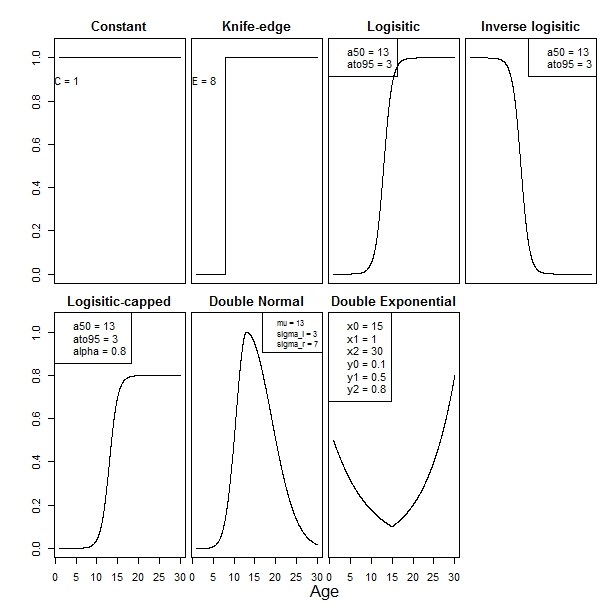
\includegraphics[scale = 0.7]{Figures/Selectivities.jpeg}
	\caption{Examples of the selectivities}
	\label{fig:select examples}
\end{figure}


\subsection{\I{Time-varying Parameter}}\label{sec:TimeVarying} \STATUS{Untested}

Any parameter can be varied annually for blocks of years or in specific years within the model run \TODO{Check: not in initialisation phases?}. For years that are not specified, the parameter will default to the input, or if in an iterative state such as estimation mode, the value being trialled at that iteration.

Method types for a time-varying parameter are:

\begin{itemize}
\item \subcommand{constant},
\item \subcommand{random\_walk},
\item \subcommand{exogenous},
\item \subcommand{linear},
\item \subcommand{annual\_shift}, and
\item \subcommand{random\_draw}.
\end{itemize}

This option allows for a parameter to be fixed in a year, or be the result of a deterministic or stochastic equation. \textbf{Note:} the stochastic time-varying functionality was added for simulation purposes. \textbf{It has not been tested in an estimation context.}

To implement hierarchical models, the prior parameter values need to be estimated using hyperpriors. To implement a hierarchical model using the time-varying functionality, use MCMC estimation as a way to calculate the integral which is required to obtain unbiased estimates. In an MCMC context, a Gibbs sampler is assumed. That is, every draw is from a conditional distribution and so every draw is a candidate value. \TODO{review}

When allowing removals with annually varying catchabilities, selectivities, and/or other model components, simulated observations more closely model real data and associated conclusions become more useful. Implementing time-varying parameters also allows for mean or location parameters of selectivities to change between years based on an explanatory variable. An example of this is in the New Zealand Hoki fishery where the $\mu$ and $a_{50}$ parameters are allowed to shift depending on when the fishing season occurs. Descriptive analysis showed that when fishing was earlier relative to other years smaller fish were caught and vice versa. This can be shown in the Examples/2stock directory, implemented at line: \texttt{382} in the \texttt{population.csl2} file. [Craig to edit]

\subsubsection[Constant (year blocks)]{\argument{constant}}\index{Time-varying Parameters!Constant}\label{sec:TimeVarying-Constant}

This option allows a parameter to have an different value during specified years to the rest of the model run,and this value can be estimated. To allow survey catchability to be different in the year block 1975 to 1988 from the rest of the series we write:

{\small{\begin{verbatim}
		@time_varying q_time_var
		type          constant
		parameter     catchability[survey_q].q
		years         1975:1988
		values        0.001      #same for all years
		\end{verbatim}}}

To estimate catchability for 1975 and 1976, use the following:

{\small{\begin{verbatim}
		@estimate q_time_var
		type uniform   #prior
		parameter time_varying[q_time_var].values{1975:1976}
		lower_bound 1e-6 1e-6
		upper_bound 2     2
		\end{verbatim}}}

To make the catchability be same over the year block we need to estimate it for one year (say 1975) and use the \textit{same} subcommand to make the others take the same value

{\small{\begin{verbatim}
		@estimate q_time_var
		type uniform
		parameter time_varying[q_time_var].values{1975}
		same      time_varying[q_time_var].values{1976:1988}
		lower_bound 1e-6
		upper_bound 2
		\end{verbatim}}}

\textbf{Caution}: do not estimate both the actual parameter and its time-varying counterpart, as the time-varying value will overwrite the actual parameter making the actual value unidentifiable. [Craig to edit]

\subsubsection[Random Walk]{\argument{random\_walk}}\index{Time-varying Parameters!Random Walk}\label{sec:TimeVarying-RandomWalk}

A random deviate drawn from a standard normal distribution is added to the previous year's value. This option has an estimable parameter $\sigma_p$ for each time-varying parameter $p$. For reproducible modelling when using stochastic functionality, set the random seed (see Section~\ref{sec:CommandLineArguments}).

{\small{\begin{verbatim}
		@time_varying q_time_var
		type          random_walk
		parameter     catchability[survey_q].q
		distribution  normal
		mean          0
		sigma         3
		\end{verbatim}}}

If the \texttt{parameter} specified in the \command{time\_varying} block is associated with an \command{estimate} block, then the parameter is constrained to stay within the lower and upper bounds of the \command{estimate} block.

\textbf{WARNING:} if the parameter does not have an associated \command{estimate} block then there is no safeguard against the application of a random deviate resulting in parameter values which cause the model to fail, i.e., generates NA or INF values. To avoid this, specify an \command{estimate} block even though the parameter is not actually being estimated; see the example syntax below.

A constraint whilst using this functionality is that a parameter cannot be less than 0.0. If it is then \CNAME\ sets it equal to 0.01.

{\small{\begin{verbatim}
		@estimate survey_q_est
		type      uniform
		parameter catchability[survey_q].q
		lower_bound 1e-6
		upper_bound 10
		\end{verbatim}}}

This configuration will insure the random walk time-varying process will set the any new candidate values within the lower and upper bound of the \command{estimate} block.

\TODO{Syntax abuse: now overloaded many parameters with just one universal one?}

\subsubsection[Annual shift]{\argument{annual\_shift}}\index{Time-varying Parameters!Annual shift} \label{sec:TimeVarying-AnnualShift}

A parameter generated in year $y$ ($\theta'_y$) depends on the value specified by the user ($\theta_y$) along with three coefficients $a$, $b$, and $c$

\begin{equation}
\bar{\theta}_y = \frac{\sum_{y}^Y\theta_y}{Y}
\end{equation}

\begin{equation}
\theta'_y = a \bar{\theta}_y + b\bar{\theta}_y^{2} + c\bar{\theta}_y^{3}
\end{equation}

\subsubsection[Exogenous]{\argument{exogenous}}\index{Time-varying Parameters!Exogenous}\label{sec:TimeVarying-Exogenous}

Parameters are shifted based on an exogenous variable. An example of this is an exploitation selectivity parameters that may vary between years based on known changes in exploitation behaviour such as season, start time, and average depth of exploitation.

\begin{equation}
\delta_y = a(E_y - \bar{E})
\end{equation}

\begin{equation}
\theta'_y = \theta_y + \delta_y
\end{equation}

where $\delta_y$ is the shift or deviation in parameter $\theta_y$ in year $y$ to generate the new parameter value in year $y$ ($\theta'_y$). $a$ is an estimable shift parameter, $E$ is the exogenous variable, and $E_y$ is the value of this variable in year $y$. For more information readers can see \cite{francis_03}.

\subsection{\I{Equation Parser}\label{sec:eq_parser}} \STATUS{Untested}

\CNAME\ has an equation parser, which is currently implemented in Projections (section~\ref{sec:Project}), Derived quantities (see Section~\ref{sec:DerivedQuantity}), and Reports (section~\ref{sec:Report}).

Examples of syntax for implementing the equation parser are below. For more information on the parser, see \url{https://github.com/nickgammon/parser/blob/master/parser.cpp}


{\small{\begin{verbatim}
		equation process[Recruitment].r0 * 2 #double the recruitment
\end{verbatim}}}

mathematical functions such as \texttt{sqrt()}, \texttt{log()},  \texttt{exp()},  \texttt{cos()}, \texttt{sin()}, and \texttt{tan()} can be used

{\small{\begin{verbatim}
		equation sqrt(process[Recruitment].r0)
\end{verbatim}}}

exponents can be used with \texttt{pow()}

{\small{\begin{verbatim}
		equation pow(2, 3)
\end{verbatim}}}

the absolute value of an equation using \texttt{abs()}

{\small{\begin{verbatim}
		equation abs(sqrt(process[Recruitment].r0) * 1.33)
\end{verbatim}}}

\texttt{if-else} statements can be used

{\small{\begin{verbatim}
		equation if(process[Recruitment].r0 > 23, 44, 55)
		## if R0 is greater than 23 return 44 else return 55
\end{verbatim}}}

\texttt{if-else} statements can also be linked, more complex syntax

{\small{\begin{verbatim}
# if R0 > 23 return 44
# else if R0 < 23 & r0 > 10 return 55
equation if(process[Recruitment].r0 > 23, 44,
         if(process[Recruitment].r0 > 10, 55, 66))
else R0 must be less than 10 return 66
\end{verbatim}}}

Only single values can be referenced, so an equation cannot be applied to a vector, e.g., \subcommand{process[Recruit].ycs\_values\{1974:1980\}} cannot be referenced. More information on which parameters can be included in an equation parser is available (Section~\ref{sec:syntax}). Any subcommand that has a \texttt{type estimable} could be referenced with the equation parser.

\textbf{Note:} the equation parser will not catch all user configuration errors, such as checking whether a parameter that exists in the system has been populated when it is required.

For example, the wrong year could be misspecified in the case of removals in year $y$ which is based on the state of the population in year $y-1$

{\small{\begin{verbatim}
		parameter process[removals].catch
		year 2015
		equation derived_quantity[percent_b0].values{2020}
\end{verbatim}}}

This example is a valid equation but it will have nonsensical results, since a value for 2020 is to be calculated using values for 2015. Although the equation parser adds flexibility, it is easy to misspecify equations.


\subsection{\I{Specifying projections}}\label{sec:Project} \STATUS{Untested}

Given a set of estimated parameter values from a \textit{-e} or a MCMC run,
the model can be projected into the future. Projection years are after the model run years, and are defined in the \textit{@model} command block using the \subcommand{final\_projection\_year} subcommand, i.e., projection years are \subcommand{final\_year + 1} through to \subcommand{final\_projection\_year}.

Parameter values for the projected years can be specified in a stochastic way or fixed at some value (the default is the estimated value if the parameter is not time-varying) and these are specified in the \textit{@projection} block,

{\small{\begin{verbatim}

@project Future_ycs  # label
type       lognormal_empirical  # which method to use
parameter  process[Recruitment].ycs_values
years      2012:2016
multiplier 1
... # any other parameters
\end{verbatim}}}

The subcommands \subcommand{years} and \subcommand{parameter} are common to all projection methods. Subcommand \subcommand{years} specifies the years to apply the new values to for the parameter in \subcommand{parameter}. Note that the years can be before the \textit{finial\_year}, e.g., it is normal to vary the last few YCS in a projection run because they are usually poorly estimated or they have been set to 1.  The argument \argument{multiplier} is a constant which is multiplied with the projected value after it has been generated. The \subcommand{type} subcommand gives the method to use to generate new parameter values.

\CNAME\ allows any estimable parameter to be specified in a \command{project} block and then varied from the estimated value in a projection. The available projection types for these parameters include:

\begin{itemize}
	\item constant
	\item lognormal
	\item empirical-lognormal
	\item empirical re-sampling
	\item user-defined
\end{itemize}

\CNAME\ has no default projection properties for parameters that are specified by year, e.g., year class strength parameters, time-varying parameters, and as a special case, future catches). For these, projections  must have a \command{project} command block. For example, \CNAME\ will produce errors if run in projection mode without a \command{project} block for the \subcommand{ycs\_values} parameter being specified.

\textbf{Note for the year class parameters:} the definition of year applies to the \argument{ycs\_years}, not the model years. As defined in Section~\ref{sec:Process-RecruitmentBevertonHolt}, \argument{ycs\_years} are offset between the time of spawning and when individuals are added to the partition.

Future catches are also specified in a \textit{@project} block, one for each fishery (see \ref{sec:Project-Catch} for examples). Here, a fishery is reference in the \textit{parameter} subcommand with the \textit{method\_} fragment to identify it,

 \textit{process[<block label>].method\_<fisheries label>},

For a process called \textit{Fishing} that has three fisheries defined, it would be \textit{process[Fishing].method\_pot} to specify the fishery labelled \textit{pot}.

The \CNAME\ command to run the model in projection mode is \texttt{Casal2 -f 1}. \TODO{review; NOT IN MANUAL OR ELSEWHERE]} This functionality allows for the exploration of many scenarios with a single set of parameters. The number of projections should be greater than 1 only if applying a projection type that is stochastic.

The \texttt{-{}-tabular} flag should be used when running projections after a Bayesian analysis. This option will output a tabular report (see Section~\ref{sec:Tabular}) which can then be analysed in \R.

An example of the command line evocation is

\textit{casal2 -f 1 -i mcmc.txt --tabular > projection.out.txt}

where \textit{mcmc.txt} is output from a MCMC run, one parameter set per row, which will give one projection per row, and \textit{projection.out.txt} will contain one row for each MCMC run in each of the reports specified in (usually) the \textit{Report.csv2} file (quantities as specified in the \textit{report.csl2} file).

For a projection run in \CNAME, the model is initialised and run through the model years from \argument{start\_year} to \argument{final\_year}. During this run mode \CNAME\ stores all parameter values so that projection classes can allow parameters before \subcommand{final\_year} to be projected. The model then is re-run from \argument{start\_year} to \argument{projection\_final\_year}, where any parameter can either be fixed or drawn from a stochastic distribution or process.


\subsubsection{\I{Projection methods}\label{sec:ProjectionMethods}}

This section lists all the projections classes available, their functionality, and an example of the syntax.

\paragraph[Constant]{The constant projection type, \argument{constant}}\index{Projections!Constant}\label{sec:Project-Constant}

A parameter can either be fixed during all projection years or specified individually for each projection year. This is a deterministic assumption, where the parameter is assumed to be known without error during projection years.

{\small{\begin{verbatim}
		@project Future_ycs
		type      constant
		parameter process[Recruitment].ycs_values
		years     2012:2016
		values    1 2 1 2 0.5  #"values 3" means all years use 3
		multiplier 1
		\end{verbatim}}}

\paragraph[Empirical sampling]{Sampling from a range of years, type  \argument{empirical\_sampling}}\index{Projections!Empirical sampling}\label{sec:Project-EmpiricalSampling}

Parameters that have time components associated with them can be sampled uniformly with replacement over a range of years and used as values for the projected years. The year range to sample from is between \argument{start\_year} and \argument{final\_year}:

{\small{\begin{verbatim}
		@project   Future_ycs
		type       empirical_sampling
		parameter  process[Recruitment].ycs_values
		years     2012:2016
		start_year 1988     # re-sample from estimated values
		final_year 2008     # from 1988 to 2008 inclusive
		multiplier 1
		\end{verbatim}}}


\paragraph[Lognormal]{Sampling from a lognormal distribution, type  \argument{lognormal}}\index{Projections!Lognormal}\label{sec:Project-LogNormal} \STATUS{Untested}

The parameters are drawn from a Gaussian distribution in log space and exponentiated  to result in the lognormal distribution

\begin{equation}\label{eq:lognormal}
X_p = exp(\epsilon_p - \sigma^2 / 2)
\end{equation}

where $\epsilon_p\stackrel{iid}{\sim}N(\mu,\sigma)$ and $X_p$ is the projected value for parameter $X$, and $\mu$ and $\sigma$ are the mean and standard deviation on the log scale.

An example of applying this process to draw future year class parameters from a lognormal distribution with mean 1 and standard deviation 0.8

{\small{\begin{verbatim}
		@project Future_ycs
		type     lognormal
		parameter process[Recruitment].ycs_values
		years     2012:2016
		mean      0     #mean 1 on un-transformed scale
		sigma     0.8   # log scale
		multiplier 1
		\end{verbatim}}}

\paragraph[Lognormal-Empirical]{Sampling from a lognormal distribution where the  variance is estimated from values over a specified year range, type  \argument{lognormal\_empirical} }\index{Projections!Lognormal-Empirical}\label{sec:Project-LogNormalEmpirical} \STATUS{Untested}

This method applies a lognormal draw as in the \argument{LogNormal} method above and specifies a year range from which the standard deviation of the distribution is calculated. Then equation~\eqref{eq:lognormal} is used to generate future values with a specified $\mu$ and empirically calculated $\sigma$,

{\small{\begin{verbatim}
		@project Future_ycs
		type      lognormal_empirical
		parameter process[Recruitment].ycs_values
		years     2012:2016
		mean      0
		start_year 1988   # range of years to take the
		final_year 2008   # values for \math{\sigma}
		multiplier 1
		\end{verbatim}}}

\paragraph[User Defined]{Sample from a user-defined function, \argument{user\_defined}}\index{Projections!User Defined}\label{sec:Project-UserDefined} \STATUS{Untested}

This method uses the equation parser to calculate the values to use in the projection. This was set up to define and apply harvest control rules (i.e., apply a management action such as changing catch limits based on the current or previous state).

In fisheries models, this option can be used to calculate the projected catch based on an exploitation rate multiplied by the vulnerable biomass, where the exploitation rate is based on a rule (Figure~\ref{fig:HCR}).

\begin{figure}[!h]
	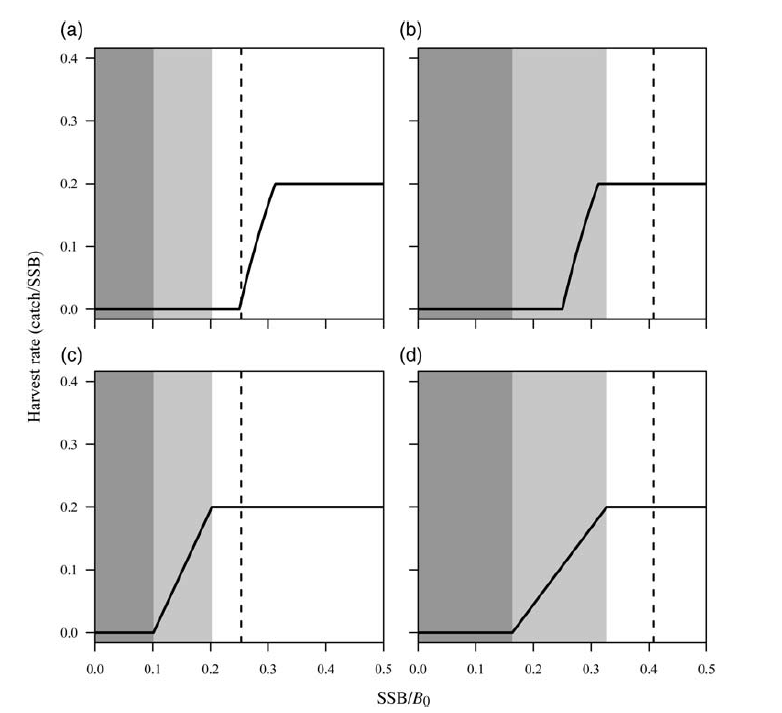
\includegraphics[scale=0.9]{Figures/HarvestControlRules.png}
	\caption{\textbf{Examples of control rules based on current stock status.}}
	\label{fig:HCR}
\end{figure}

\pagebreak
{\small{\begin{verbatim}
		@project HCR_2015
		type       user_defined
		parameter process[Instantaneous_Mortality].method_Sub_Ant_F
		years 2015
		equation if(derived_quantity[SSB].values{2014} / process[Recruitment].b0 <= 0.1, 0.0,
		if(derived_quantity[SSB].values{2014} / process[Recruitment].b0 > 0.1 &&
		derived_quantity[SSB].values{2014} / process[Recruitment].b0 < 0.2,
		derived_quantity[SSB].values{2014} * derived_quantity[SSB].values{2014}
		/ process[Recruitment].b0,
		derived_quantity[SSB].values{2014} * 0.2))
		\end{verbatim}}}

Care should be taken when writing user-defined equations. The above equation is: if $\%B_{2014} \leq 0.1$ then set next year's catch to 0.0, else if $\%B_{2014} > 0.1 \text{ } \& \text{ } \%B_{2014} \leq 0.2$ then set next year's catch equal to $\%B_{2014} \times SSB_{2014}$, else set next year's catch to $0.2 SSB_{2014}$.

\paragraph[Catches]{Specifying catch for projections }\index{Projections!Catches}\label{sec:Project-Catch}

Catches are unique in that they are known inputs in a table format. For example, to project catches that are in a table

{\small{\begin{verbatim}
# fishing process
@process Fishing
type mortality_instantaneous_retained
m 0.17*6  #0.17    #testing at old values
time_step_proportions 1
relative_m_by_age One*6   #for age based M
categories *
table catches
year	FishingLine	FishingPot	Recreation
1900	0	0	0
1901	13.2	0	22.9
1902	26.4	0	23.5
1903	39.6	0	24
end_table

# projection block
@project future_catch
type      constant
parameter process[Fishing].method_fishingpot
years     2020:2029
values    4000
\end{verbatim}}}

This uses the syntax \texttt{block\_type[block\_label].method\_fishinglabel}. \textbf{Note:} the fishing label which is defined in the table needs to be lower case form in the \command{projection} block. Notice the use of \textit{method\_} syntax to identify the right fishery.


\clearemptydoublepage{}
\section{\I{The estimation section: estimation methods and parameters}\label{sec:Estimation}}

The command and subcommand syntax for the estimation section is given in Section \ref{syntax:Estimation}.

\subsection{\I{Role of the estimation section}\label{sec:role-of-the-estimation-section}}

The role of the estimation section is to define the tasks carried out by \CNAME:

\begin{enumerate}
  \item Define the objective function (see Section \ref{sec:objective-function})
  \item Define the parameters to be estimated (the free parameters, see Section \ref{sec:FreeParameters})
  \item Calculate a point estimate, i.e., the maximum posterior density estimate (MPD) (see Section \ref{sec:estimate-MPD})\index{Maximum posterior density estimate (MPD)}\index{MPD (Maximum posterior density estimate)}
  \item Calculate a posterior profile on selected parameters, i.e., for each of a series of values of a parameter, minimise the objective function, allowing the other estimated parameters to vary (see Section \ref{sec:Profile}\index{Profiles})
  \item Generate MCMC\index{Markov chain Monte Carlo (MCMC)} samples from the posterior distribution (see Section \ref{sec:MCMC}\index{MCMC})
  \item Calculate the approximate covariance matrix of the parameters as the inverse of the minimizer\textquoteright{}s approximation to the \I{Hessian}, and the corresponding correlation matrix (see Section \ref{sec:estimate-MPD}\index{Covariance matrix})
\end{enumerate}

The estimation section defines the objective function, parameters of the model, and the method of estimation (point estimates, Bayesian posteriors, profiles, etc.). The objective function is based on a goodness-of-fit measure of the model to observations, the assumed priors, and the penalties. See the observation section for a description of the observations, likelihoods, priors, and penalties.

\subsection{\I{The objective function}\label{sec:objective-function}}

In Bayesian estimation, the objective function is a negative log-posterior,

\begin{equation}\label{objective_function}
Objective(p)= - \sum\limits_i {\log \left[ {L\left( {{\bf{p}}|O_i } \right)} \right]}  - \log \left[ {\pi \left( {\bf{p}} \right)} \right]
\end{equation}

where $\pi$ is the joint prior density of the parameters $p$.

The contribution to the objective function from the likelihood components is described in Section \ref{sec:Likelihood}. In addition to likelihoods, priors (see Section \ref{sec:Priors}) and penalties (see Section \ref{sec:Penalty}) are components of the objective function. Note that if the priors are specified as uniform, then the prior contribution is zero and the optimisation is now a penalised likelihood and not Bayesian.

Penalties can be used to ensure that the estimated parameter values and derived quantities meet certain restrictions. For example, exploitation rate constraints on mortality events (i.e., fisheries) that are not violated (otherwise there is nothing to prevent the model from having abundances so low that the recorded catches could not have been taken); penalties on category transitions (to ensure there are enough individuals to move); penalties such that estimated values are similar or smooth, etc.

Equation~\ref{objective_function} can be reduced to a penalised likelihood equation if all priors are assumed to be uniform. This is because uniform priors have no contribution to the objective function so Equation~\ref{objective_function} reduces to the likelihood components plus penalties.

\subsection{\I{Specifying the parameters to be estimated}\label{sec:FreeParameters}}

The parameters to be estimated (estimables) are defined using \command{estimate} commands (see Section \ref{syntax:Estimation}).

For example, a \command{estimate} command block \index{Estimating parameters}

{\small{\begin{verbatim}
  @estimate male.m
  parameter process[NaturalMortality].m{male}
  lower_bound 0.1
  upper_bound 0.4
  type uniform
\end{verbatim}}}

See Section \ref{sec:parameter-names} for information on how to specify the parameter name. At least one parameter is required to be estimated if doing an estimation \texttt{-e}, profile \texttt{-p}, or MCMC \texttt{-m} run. Initial values for the parameters to be estimated are required, and these values are used as the starting values for the minimiser. However, these values may be overwritten if a set of alternative starting values is provided (i.e., using \texttt{\cname\ -i}, see Section \ref{sec:CommandLineArguments}).

All parameters are estimated within the specified bounds\index{Bounds}. For each parameter estimated, the lower and upper bounds and the prior\index{Priors} (\texttt{type}) (Section \ref{sec:Priors}) must be specified. The bounds and the prior should be chosen carefully as they affect the values over which the minimisers search. Some minimisers convert the lower and upper bounds into a minimisation space (for example -1,1 space for the numerical differences algorithm). If estimating only some elements of a vector, either define each element of the vector to be estimated or fix the others by setting the the lower and upper bounds to the same value as the initial value.

\subsection{\I{Point estimation}\label{sec:estimate-MPD}}\label{sec:Minimiser}

Point estimation is invoked with \texttt{\cname\ -e}, which attempts to find a minimum of the objective function\index{Objective function}. \CNAME\ has multiple minimisation algorithms. There are two automatic differentiation (AD) minimisers: ADOL-C, and BetaDiff (the minimiser used in CASAL). There are also three non-automatic differentiation minimisers: numerical differences, DeltaDiff, and the differential evolution minimiser (\subcommand{de\_solver}). Automatic differentiation  minimisers are recommended for more complex models as they are on average much faster and tend to find a more robust minimum when exploring a complex objective surface.

An important input parameter for most minimisers is the \subcommand{tolerance} parameter. This is the gradient of the objective function, and is used as the stopping rule to define the 'solution' (although a solution may be a local minimum and not the global minimum). Evaluating the robustness of a minimum can be tested with different starting values (i.e., using \texttt{-i free\_parameter\_file.txt}).

Start with the default \subcommand{tolerance} parameter value of 1e-5 and decrease it while developing a model. For a given model, the parameter estimates when minimising with different tolerance may be different.

\subsubsection{\I{The numerical differences minimiser}}\label{sec:Minimiser-GammaDiff}

See Section \ref{syntax:Minimiser-GammaDiff} for the command syntax.

The numerical differences minimiser uses a quasi-Newton minimiser which is a slightly modified implementation of the main algorithm of \cite{779}, and uses an $arcsin$ transformation to ensure parameters remain within bounds.

The minimiser has three kinds of (non-error) exit status, depending on the minimiser:

\begin{itemize}
\item Successful convergence (suggests a local minimum has been found, at least).
\item Convergence failure (a local minimum has not been found, although the results may be 'close enough').
\item Convergence unclear (the minimiser halted but was unable to determine if convergence occurred. The result may be a local minimum, although this can be checked by restarting the minimiser at the final values of the estimated parameters).
\end{itemize}

The maximum number of quasi-Newton iterations\index{Quasi-Newton iterations} and objective function evaluations\index{Objective function evaluations} allowed can be specified. If either limit is exceeded, the minimiser exits with a convergence failure\index{Convergence failure}. Set the maximum number of evaluations and iterations to values larger than the defaults of 300 and 1000, unless convergence is reached with fewer. An alternative starting point of the minimiser can be specified using \texttt{\cname\ -i}.

The minimisers are local optimisation algorithms trying to solve a global optimisation problem. What this means is that, even if a 'successful convergence'\index{Successful convergence} is reached, the solution may be only a local minimum\index{Local minimums}, and not a global one. To diagnose this problem, start multiple runs from different starting points and comparing the results, or do profiles of one or more key parameters and seeing if any of the profiled estimates finds a better optimum than than the original point estimate.

The approximate covariance matrix\index{Covariance matrix} of the estimated parameters can be calculated as the inverse of the minimiser's approximation to the \I{Hessian}, and the corresponding correlation matrix\index{Correlation matrix} is also calculated.

Note that

\begin{itemize}
\item the Hessian approximation develops over many minimiser steps, so if the minimiser has only run for a small number of iterations the covariance matrix can be a very poor approximation; and
\item the inverse Hessian is not a good approximation to the covariance matrix of the estimated parameters, and may not be useful to construct, for example, confidence intervals.
\end{itemize}

Also note that if an estimated parameter has equal lower and upper bounds, it will have entries of '0' in the covariance matrix and \texttt{NaN} or \texttt{-1.\#IND} (depending on the operating system) in the correlation matrix.

{\small{\begin{verbatim}
@minimiser numerical_diff
type numerical_differences
tolerance 1e-6
iterations 2500
evaluations 4000
\end{verbatim}}}

\subsubsection{\I{The DeltaDiff numerical differences minimiser}}\label{sec:Minimiser-DeltaDiff}

See Section \ref{syntax:Minimiser-DeltaDiff} for the command syntax.

DeltaDiff applies the same minimiser as Numerical Differences, expect that it uses $tan$ rescaling for the parameters rather than $arcsin$. This minimiser may perform better than the Numerical Differences minimiser when parameters are very close to zero bounds.

\subsubsection{\I{The differential evolution minimiser}}\label{sec:Minimiser-DESolver}

The differential evolution minimiser is a simple population-based, stochastic function minimizer, but is claimed to be quite powerful in solving minimisation problems. It is a method of mathematical optimization of multidimensional functions and belongs to the class of evolution strategy optimizers.

Initially, the procedure randomly generates and evaluates a number of solution vectors (the population size), each with $p$ parameters. Then, for each generation (iteration), the algorithm creates a candidate solution for each existing solution by random mutation and uniform crossover. The random mutation generates a new solution by multiplying the difference between two randomly selected solution vectors by some scale factor, then adding the result to a third vector. Then an element-wise crossover takes place with probability $P_{cr}$, to generate a potential candidate solution. If this is better than the initial solution vector, it replaces it, otherwise the original solution is retained. The algorithm terminates after either a predefined number of generations (\argument{max\_generations}) or when the maximum difference between the scaled individual parameters from the candidate solutions from all populations is less than some predefined amount \argument{tolerance}.

The differential evolution minimiser can be good at finding global minimums in surfaces that may have local minima. However, the speed of the minimiser, and the ability to find a good minima depend on the number of initial 'populations'. Some authors recommend that the number of populations be set at about $10*p$, where $p$ is the number of free parameters. However, depending on the model, this value can be set to a lower value and still find a robust solution.

There is no proof of convergence for the differential evolution solver, but several papers have found it to be an efficient method of solving multidimensional problems. Some results suggest that it can often find a better minima and may be faster or longer (depending on the actual model specification) at finding a solution when compared with the numerical differences minimiser. Comparisons with automatic differentiation minimisers or other more sophisticated algorithms have not been made.

{\small{\begin{verbatim}
		@minimiser DE_solver
		type de_solver
		tolerance 1e-6
		iterations 2500
		evaluations 4000
\end{verbatim}}}

\subsubsection{\I{The BetaDiff minimiser}}\label{sec:Minimiser-BetaDiff}

An automatic differentiation minimiser for non-linear models, This is the minimiser from the original CASAL package, based on ADOL-C.

{\small{\begin{verbatim}
		@minimiser beta_diff
		type beta_diff
		tolerance 1e-6
		iterations 2500
		evaluations 4000
\end{verbatim}}}

\subsubsection{\I{The ADOL-C minimiser}}\label{sec:Minimiser-ADOLC}

An automatic differentiation minimiser for non-linear models. See \url{https://projects.coin-or.org/ADOL-C} for more information. Users do have an option of defining what transformation to apply to convert the parameter \(\theta \in [\theta_{LB}, \theta_{UB}]\) to \(X \in [-1, 1]\), for which optimisation is done. The options are sin or tan. Initial model runs suggest this assumption will make a difference to convergence, particularly if there are poorly identified parameters which fall at the bounds, we have found the sin transform is more consistent with the betadiff minimser. The sin transform
\begin{equation}
	X = \frac{asin(2 * (\theta - \theta_{LB}) / (\theta_{UB} - \theta_{LB}) - 1)}{ 1.57079633}
\end{equation}
%
the real consequence of this transformation is when \(X\) is back transformed to \(\theta\) there is a penalty which is added to the minimisation to dissuade parameter values close to the bounds. This penalty is hidden from the reported objective function. If you are interested in it, you can run with \texttt{--loglevel medium} and it should be reported. The back transformation follows,
\begin{equation}
\theta = \theta_{LB} + (\theta_{UB} - \theta_{LB}) * (sin(X * 1.57079633) + 1) / 2;
\end{equation}
%
and penalty
\begin{align}
	&if(-0.9999 - X < 0) & penalty += (X + 0.9999)^2\\
	&if(X - 0.9999 < 0) & penalty += (X - 0.9999)^2
\end{align}
%
This can be seen here \href{https://github.com/NIWAFisheriesModelling/CASAL2/blob/1b1ed731537dc551674c911da3bf387273a97a92/CASAL2/source/Utilities/Math.h#L245}{here}.


The Tan transform uses transformation

\begin{equation}
X = tan(((\theta - \theta_{LB}) / (\theta_{UB} - \theta_{LB}) - 0.5) * \pi)
\end{equation}
%
and back transform
\begin{equation}
\theta = ((atan(X) / \pi) + 0.5) * (\theta_{UB} - \theta_{LB}) + \theta_{LB}
\end{equation}

{\small{\begin{verbatim}
		@minimiser ADOLC
		type adolc
		step_size 1e-6
		iterations 2500
		evaluations 4000
		tolerance 1e-6
		parameter_transformation sin_transform
\end{verbatim}}}

\subsection{\I{Posterior profiles}}\label{sec:Profile}

If profiles are run using the command \texttt{\cname\ -p}, \CNAME\ will first calculate a point estimate. For each scalar parameter or, in the case of vectors or selectivities, the element of the parameter to be profiled, \CNAME\ will fix its value at a sequence of $n$ evenly spaced numbers ($step$) between the specified lower and upper bounds $l$ and $u$, and calculate a point estimate at each value.

By default $step=10$, and $(l, u)=($lower bound on parameter plus $(range/(2n))$, upper bound on parameter less $(range/(2n))$. Each minimisation starts at the final parameter values from the previous resulting value of the parameter being profiled. \CNAME\ will report the objective function for each parameter value. The initial point estimate should be compared with the profile results, to check at least that none of the other points along the profile have a better objective function value than the initial 'minimum'.

The parameters to be profiled are specified, and optionally the number of steps, and lower bound and upper bound, for each parameter. In the case of vector parameters, the element(s) of the vector to be profiled are specified.

The initial starting point for the estimation can also be specified using \texttt{\cname\ -i \emph{file}}, which may improve the minimiser performance for the profiles.

If the profile results are not reasonable, it may be a result of not using enough iterations in the minimiser or a poor choice of minimiser control variables (e.g., the minimiser tolerance). It may also be useful to try other minimisers and compare the results.

\subsection{\I{Bayesian estimation}}\label{sec:MCMC}\label{sec:MCMC-RandomWalkMetropolisHastings}

\CNAME\ can use \I{Markov chain Monte Carlo (MCMC)}\index{MCMC} functionality to generate a sample from the posterior distribution of the estimated parameters with command \texttt{\cname\ -m} and output the sampled values to a file, optionally keeping only every $n$th set of values.

As \CNAME\ has no post-processing capabilities. \CNAME\ cannot produce MCMC convergence diagnostics. To calculate these diagnostics, use a package such as \href{http://www.public-health.uiowa.edu/boa}{BOA}, plot/summarize the posterior distributions of the output quantities, and/or use a general-purpose statistical package such as \href{http://www.r-project.org}{\R}.

Bayesian methodology\index{Bayesian estimation} and MCMC are both large and complex topics. See Gelman et al. \citeyearpar{823} and Gilks et al. \citeyearpar{143} for details of both Bayesian analysis and MCMC methods. In addition, see Punt \& Hilborn \citeyearpar{828} for an introduction to quantitative fish stock assessment using Bayesian methods.

This section briefly describes the MCMC algorithms used in \CNAME. See Section \ref{syntax:MCMC} for the \CNAME\ commands used in an MCMC Bayesian analysis.

\CNAME\ implements two methods for MCMC. The first is a straightforward implementation of the random walk Metropolis-Hastings algorithm \citep{823,143}. The Metropolis-Hastings algorithm attempts to draw a sample from a Bayesian posterior distribution, and calculates the posterior density $\pi$, scaled by an unknown constant. The algorithm generates a 'chain' or sequence of values. Typically the beginning of the chain is discarded (the burn-in period) and every $N$th element of the remainder is taken as the posterior sample. The second is Hamiltonian Monte Carlo. This uses similar subcommands as the random walk Metropolis-Hastings algorithm. In both cases, the chain is produced by taking an initial point $x_0$ and repeatedly applying the following rule, where $x_i$ is the current point:

\begin{enumerate}
\item Draw a candidate step s from a proposal distribution J, which should be symmetric i.e., $J(-s)=J(s)$
\item Calculate $r=min(\pi(x_i+s)/\pi(x_i),1)$
\item Let $x_{i+1}=x_i+s$ with probability $r$, or $x_i$ with probability $1-r$
\end{enumerate}

An initial point estimate is produced before the chain starts, which is done so as to calculate the approximate covariance matrix of the estimated parameters (as the inverse Hessian), and may also be used as the starting point of the chain.

The starting point of the point estimate minimiser can be specified using the command \texttt{\cname\ -i}. Don't start it too close to the actual estimate (either by using \texttt{\cname\ -i}, or by changing the initial parameter values in \config) as it takes a few iterations to determine a reasonable approximation to the Hessian.

There are currently two options for the starting point of the MCMC:

\begin{itemize}
\item Start from the point estimate; or
%\item Start from a random point near the point estimate (the point is generated from a multivariate normal distribution, centred on the point estimate, with covariance equal to the inverse Hessian multiplied by a user-specified constant). This may be useful if the chain gets `stuck' at the point estimate, or if you wish to generate multiple chains from  for later MCMC diagnostic tests.
\item Restart a chain given a covariance matrix and a previous starting point.
\end{itemize}

The chain moves in natural space, i.e., no transformations are applied to the estimated parameters. The default proposal distribution is a multivariate Student's $t$ distribution centred on the current point, with covariance matrix equal to a matrix based on the approximate covariance produced by the minimiser, multiplied by a step size factor.

The following steps define how the initial covariance matrix of the proposal distribution is calculated:

\begin{enumerate}
\item The covariance matrix is taken as the inverse of the approximate Hessian from the quasi-Newton minimiser.

\item The covariance matrix is modified so as to decrease all correlations greater than \commandsub{mcmc}{max\_correlation} down to \commandsub{mcmc}{max\_correlation}, and similarly to increase all correlations less than -\commandsub{mcmc}{max\_correlation} up to -\commandsub{mcmc}{max\_correlation} (the \commandsub{mcmc}{max\_correlation} parameter defaults to 0.8). This should help to avoid getting 'stuck' in a lower-dimensional subspace.

\item The covariance matrix is then modified either by

\begin{itemize}
\item  \commandsubarg{mcmc}{adjustment\_method}{covariance}: that if the variance of the $i$th parameter is non-zero and less than \commandsub{mcmc}{min\_difference} multiplied by the difference between the parameters' lower and upper bound, then the variance is changed, without changing the associated correlations, to $k=$min\_diff$(upper\_bound_i-lower\_bound_i)$. This is done by setting \[
{\mathop{\rm Cov}\nolimits} \left( {i,j} \right)^\prime   = {{{\mathop{\rm sqrt}\nolimits} \left( k \right){\mathop{\rm Cov}\nolimits} \left( {i,j} \right)} \mathord{\left/
{\vphantom {{{\mathop{\rm sqrt}\nolimits} \left( k \right){\mathop{\rm Cov}\nolimits} \left( {i,j} \right)} {{\mathop{\rm sd}\nolimits} \left( i \right)}}} \right.
\kern-\nulldelimiterspace} {{\mathop{\rm sd}\nolimits} \left( i \right)}}
\]
for $i \ne j$, and ${\mathop{\rm var}} \left( i \right)^\prime   = k$

\item \commandsubarg{mcmc}{adjustment\_method}{correlation}: that if the variance of the $i$th parameter is non-zero and less than \commandsub{mcmc}{min\_difference} multiplied by the difference between the parameters' lower and upper bounds, then its variance is changed to $k=min\_diff(upper\_bound_i-lower\_bound_i)$. This differs from (i) above in that the effect of this option is that it also modifies the resulting correlations between the $i$th parameter and all other parameters.
\end{itemize}

This allows each estimated parameter to move in the MCMC even if its variance is very small according to the inverse Hessian. In both cases, the \commandsub{mcmc}{min\_difference} parameter defaults to $0.0001$.

\item The \commandsub{mcmc}{stepsize} (a scalar factor applied to the covariance matrix to improve the acceptance probability) is set by the user. The default is $2.4d^{-0.5}$ where $d$ is the number of estimated parameters, as recommended by Gelman et al. \citep{823}.
\end{enumerate}

The proposal distribution can also change adaptively during the chain, using two different mechanisms. Both are offered as means of improving the convergence properties of the chain. It is important to note that any adaptive behaviour must finish before the end of the burn-in period, i.e., the proposal distribution must be finalised before the kept portion of the chain starts.

The adaptive mechanisms are:

\begin{itemize}
\item The step size changes adaptively at one or more sample numbers (See next paragraph for details on the step size adaptation methods)
\item The entire covariance matrix changes adaptively at one or more sample numbers. At each adaptation, the covariance matrix is replaced with an empirical covariance matrix, derived from the MCMC chain. The idea is that an empirical covariance is a better approximation of the proposal distribution than the inverse of the Hessian matrix, and can improve convergence and mixing of the chain.
\end{itemize}

The two options to adapt the step size are \texttt{double\_half} or \texttt{ratio}, which is chosen with the input parameter \texttt{adapt\_stepsize\_method}. The \texttt{double\_half} method is used in CASAL (see Gelman et al. \citep{823} for justification).

The algorithm for \texttt{double\_half} is, at each adaptation, the step size is doubled if the acceptance rate since the last adaptation is more than $0.5$, or halved if the acceptance rate is less than $0.2$. The \texttt{ratio} is taken from SPM. It adapts the current step size by the acceptance rate since the last adaptation multiplied by 4.1667 to approach an acceptance rate of $\approx$ 0.24. See \cite{mcmc_rate} for justification on that acceptance rate.

The \texttt{stepsize} parameter is now on a completely different scale, and must be rescaled. It is set to a user-specified value (which may or may not be the same as the initial step size). Set the step size adaptations to occur after this, so that the step size can be readjusted to an appropriate value which gives good acceptance probabilities with the new matrix.

All modified versions of the covariance matrix are printed to the standard output, but only the initial covariance matrix (inverse Hessian) is saved to the objectives file. The number of covariance modifications by each iteration is recorded as a column on the objectives file.

The variance-covariance matrix of this sub-sample of chain is calculated. As above, correlations greater than \commandsub{mcmc}{max\_correlation} are reduced to \commandsub{mcmc}{max\_correlation}, correlations less than -\commandsub{mcmc}{max\_correlation} are increased to  -\commandsub{mcmc}{max\_correlation}, and very small non-zero variances are increased (\commandsub{mcmc}{covariance\_adjustment} and \commandsub{mcmc}{min\_difference}). The result is the new variance-covariance matrix of the proposal distribution.

The procedure used to choose the sample of points is that, to start, all points on the chain so far are taken. \TODO{reword this paragraph} All points in an initial user-specified period are discarded. The assumption is that the chain will have started moving during this period. If this is incorrect and the chain has still not moved by the end of this period, it is a fatal error and \CNAME\ stops. The remaining set of points must contain at least some user-specified number of transitions. If this is incorrect and the chain has not had at least this number of transitions, then it is also a fatal error. If this test is passed, the set of points is systematically sub-sampled down to 1000 points (and it must be at least this long to start with).

The probability of acceptance for each jump is $0$ if the jump would move a parameter value outside of its bounds, $1$ if it improves the posterior, or $(new posterior/old posterior)$ otherwise. How often the position of the chain is recorded is specified with the \texttt{keep} parameter. For example, with \texttt{keep 10}, only every $10$th sample is recorded.

The option to specify that some of the estimated parameters are fixed during the MCMC is available. If the chain starts at the point estimate or at a random location, these fixed parameters are set to their values at the point estimate.

If  the start of the chain is specified with the command \texttt{\cname\ -i}, these fixed parameters are set to the values in the file.

Restarting an MCMC chain: in the case where an MCMC chain was halted or interrupted, the MCMC chain can be restarted from where it finished with

{\small{\begin{verbatim}
casal2 -R MPD_file --objective-file objectives_file --sample-file samples_file
\end{verbatim}}}

where \texttt{Objective\_file\_name} is the file name for the objective function report and \texttt{Sample\_file\_name} is the file name for the sample report from a MCMC chain.

The posterior sample can be used for (projections (Section \ref{sec:Project})) or simulations (see Section \ref{sec:Simulate}) with the values supplied with the command \texttt{\cname\ -i \emph{file}}.

A multivariate Student's $t$ distribution is used as an alternative to the multivariate normal proposal distribution. If you request multivariate Student's $t$ proposals, change the degrees of freedom from the default of 4. As the degrees of freedom decreases, the $t$ distribution becomes more heavy tailed. This may lead to better convergence properties. Note the default is the multivariate Student's $t$.

Given a posterior (sub)sample, \CNAME\ can calculate a list of output quantities for each sample point (see Section~\ref{sec:Report} specifically tabular report). These quantities can be output to a file (with the command \texttt{\cname\ -r --tabular}) and read into an external software package where the posterior distributions can be plotted and/or summarised.

The posterior sample can also be used for projections (Section~\ref{sec:Project}). The advantage of this is that the parameter uncertainty, as expressed in the posterior distribution, can be included into the risk estimates.

\subsection{Priors\label{sec:Priors}}

In a Bayesian analysis, a prior is required for every parameter that is being estimated. There are no default priors.

When some of these priors are parameterised in terms of mean, c.v., and standard deviation, these refer to the parameters of the distribution before the bounds are applied. The moments of the prior after the bounds are applied may differ.

\CNAME\ has the following priors (expressed in terms of their contribution to the objective function):


\subsubsection{Uniform\index{Uniform prior}\index{Priors ! Uniform}}\label{sec:Prior-Uniform}

\begin{equation}
 - \log \left(\pi \left(p \right) \right) = 0
\end{equation}

\subsubsection{Uniform-log\index{Uniform-log prior}\index{Priors ! Uniform-log}} (i.e., $\log(p) \sim \text{uniform}$)\label{sec:Prior-UniformLog}

\begin{equation}
 - \log \left(\pi \left(p \right) \right) = \log \left( p \right)
\end{equation}

\subsubsection{Normal\index{Normal prior}\index{Priors ! Normal}}\label{sec:Prior-Normal}

The normal distribution with mean $\mu$ and standard deviation with c.v $c$

\begin{equation}
 - \log \left(\pi \left(p \right) \right) = 0.5\left(\frac{p - \mu}{c\mu} \right)^2
\end{equation}

\subsubsection{Normal with standard deviation}\label{sec:Prior-NormalByStdev}

The normal distribution with mean $\mu$ and standard deviation $\sigma$

\begin{equation}
 - \log \left(\pi \left(p \right) \right) = 0.5\left(\frac{p - \mu}
{\sigma }\right)^2
\end{equation}

\subsubsection{Lognormal\index{Lognormal prior}\index{Priors ! Lognormal}}\label{sec:Prior-Lognormal}

The lognormal distribution with mean $\mu$ and c.v. $c$

\begin{equation}
 - \log \left(\pi \left(p \right) \right) = \log \left( p \right) + 0.5 \left( \frac{\log \left( p / \mu \right)}{s} + \frac{s}{2} \right)^2
\end{equation}

where $s$ is the standard deviation of $\log(p)$ and $s= \sqrt{\log \left(1+c^2 \right)}$.

\subsubsection{Normal-log\index{normal-log prior}\index{Priors ! Normal-log}}\label{sec:Prior-NormalLog}

The normal-log distribution  with mean $\mu$ and c.v. $c$

Similar to the lognormal prior, but with the mean ($mu$) and standard deviation ($sigma$) specified in log space.

where $s$ is the standard deviation of $\log(p)$ and $s= \sqrt{\log \left(1+c^2 \right)}$.


\subsubsection{Beta\index{Beta prior}\index{Priors ! Beta}}\label{sec:Prior-Beta}

The Beta distribution with mean $\mu$ and standard deviation $\sigma$, and range parameters $A$ and $B$

\begin{equation}
 - \log \left(\pi \left( p \right) \right) = \left( 1 - m \right) \log \left( p - A \right) + \left( 1 - n \right)\log \left( B - p \right)
\end{equation}

where $\nu  = \frac{\mu  - A}{B - A}$, and $\tau = \frac{\left(\mu -A \right)\left(B - \mu \right)}{\sigma ^2} - 1$ and then $\mu=\tau \nu$ and $n=\tau(1-\nu)$. Note that the beta prior is undefined when $\tau \leq 0$.

Vectors of parameters can be independently (but not necessarily identically) distributed according to any of the above forms, in which case the joint negative-log-prior for the vector is the sum of the negative-log-priors of the components. Values of each parameter need to be specified for each element of the vector. Example of syntax to define the estimation of a parameter and the prior assumed:

{\small{\begin{verbatim}
		## uniform-log example estimate
		@estimate B0
		type uniform_log	# this command "type" defines the prior type.
		parameter process[Recruitment].b0 # "Recruitment" is the label of your process
		upper_bound 20000
		lower_bound 1000

		## Lognormal YCS estimation
		@estimate year_class_strengths_1990_1995
		type lognormal
		parameter process[Recruitment].ycs_values{1990:1995}
		# ycs_year  1990	1991	1992	1993	1994	1995
		mu   		1   	1   	1   	1   	1   	1
		cv 			0.9 	0.9 	0.9 	0.9 	0.9 	0.9
		lower_bound 0.01	0.01	0.01	0.01	0.01	0.01
		upper_bound 9		9		9		9		9		9
\end{verbatim}}}

\subsection{Penalties}\label{sec:Penalty}\label{sec:Penalty-Process}

Penalties are associated with processes and can be used to enforce parameter value or derived quantity restrictions or model outputs that are invalid by adding a penalty to the objective function. For example, estimated parameter values can be restricted so that a known mortality event removes enough individuals from the population within an event mortality process. \CNAME\ requires penalty functions for processes that remove or shift a \emph{number} of individuals between categories or from the partition. Many of the penalties that were available in CASAL have been moved to be additional priors in \CNAME (see Section~\ref{sec:AdditionalPriors}).

For penalties, a multiplier is required to be specified, and the objective function is increased by this multiplier multiplied by the penalty value. In some cases the multiplier may need to be quite large to prohibit some model behaviour.

Penalties are implemented for the processes

\begin{itemize}
	\item \commandlabsubarg{process}{type}{event\_mortality},
	\item \commandlabsubarg{process}{type}{mortality\_instantaneous},
	\item \commandlabsubarg{process}{type}{tag\_by\_length},
	\item \commandlabsubarg{process}{type}{tag\_by\_length}, and
	\item \commandlabsubarg{process}{type}{category\_transition}
\end{itemize}

For these processes, two types of penalties can be defined: on the natural scale (the default) and on the log scale. Both of these types add a penalty value of the squared difference between the observed value (e.g., the actual number of individuals to be removed in an event mortality process or the actual number of individuals to shift in a category transition process), and the number that were moved (if less than or equal), multiplied by the penalty multiplier.

The natural scale penalty calculates the squared difference on a natural scale, and the log scale penalty calculates the squared difference of the logged values.

For example:

{\small{\begin{verbatim}
@process Mortality
type mortality_instantaneous
penalty CatchMustBeTaken

# define the penalty in an @penalty block
@penalty CatchMustBeTaken
type process
log_scale True
multiplier 10000
\end{verbatim}}}

Penalties are added to the objective function in the following ways;

\begin{equation}
	Penalty = (X_1 - X_2)^2
\end{equation}

or if \subcommand{log\_scale true}

\begin{equation}
Penalty = (log(X_1) - log(X_2))^2
\end{equation}

where, for example, $X_1$ is observed catch biomass and $X_2$ is the estimated catch biomass. Penalties are usually applied in situations when numbers or weight are known. Another example is for tagging, where the number of individuals that were tagged in a given year is known, so a penalty can be used to restrict the model to estimate reasonable values for the numbers of tagged individuals in that year.

\subsection{Additional Priors\label{sec:AdditionalPriors}}

Additional priors can be thought of as the inverse of penalties \TODO{please rephrase}. For CASAL models, most of the legacy \command{penalty} blocks have now been implemented as \command{additional\_prior} blocks. They restrict parameters in user-defined spaces \TODO{please rephrase}.

The types of additional priors available in \CNAME\ are \texttt{vector\_smoothing}, \texttt{vector\_averaging}, \texttt{uniform\_log}, \texttt{lognormal}, \texttt{element\_difference}, and \texttt{Beta}:

\begin{itemize}
	\item \texttt{vector\_average}\label{sec:AdditionalPrior-VectorAverage}

	This prior can be applied to a vector parameter. Sum of squares of $r^{th}$ differences, optionally on a log scale. This encourages the vector to be like a polynomial of degree $(r-1)$. A range of the vector to be "smoothed" can be specified (and if not, the smoother is applied to the entire vector). However, this restriction must be specified by an index of the vector and must be between 1 and the length of the vector, inclusive.

	\item \texttt{vector\_smoothing}\label{sec:AdditionalPrior-VectorSmoothing}

	This prior can be applied to a vector parameter. Square of (mean(vector)-k), or of (mean(log(vector))-l), or of (log(mean(vector)/m)). Restricts the vector to average arithmetically to k or m, or geometrically to exp(l). Typically used for YCS with k=1 or m=1 or l=0, to restrict the YCS to centre on 1. Optionally, indices can be chosen or excluded outside a given set of bounds.

	\item\texttt{lognormal} with mean $\mu$ and c.v. $c$\label{sec:AdditionalPrior-LogNormal}

	\begin{equation}
	- \log \left(\pi \left(p \right) \right) = \log \left( p \right) + 0.5 \left( \frac{\log \left( p / \mu \right)}{s} + \frac{s}{2} \right)^2
	\end{equation}

	\item\texttt{uniform\_log}\label{sec:AdditionalPrior-UniformLog}

	\begin{equation}
	- \log \left(\pi \left(p \right) \right) = \log \left( p \right)
	\end{equation}

	\item\texttt{element\_difference}\label{sec:AdditionalPrior-ElementDifference}

	\begin{equation}
	- \log \left(\pi \left(p_1,p_2 \right) \right) = \sum_{i = 1}^n \left( p_{1,i} - p_{2,i} \right)^2
	\end{equation}

	\item\texttt{Beta}\label{sec:AdditionalPrior-Beta}

	{Beta\index{Beta additional prior}\index{Additional Priors ! Beta} with mean $\mu$ and standard deviation $\sigma$, and range parameters $A$ and $B$, for parameter value = $p$}

	\begin{equation}
	- \log \left(\pi \left( p \right) \right) = \left( 1 - m \right) \log \left( p - A \right) + \left( 1 - n \right)\log \left( B - p \right)
	\end{equation}

	where $\nu  = \frac{\mu  - A}{B - A}$, and $\tau = \frac{\left(\mu -A \right)\left(B - \mu \right)}{\sigma ^2} - 1$ and then $m=\tau \nu$ and $n=\tau(1-\nu)$. The beta prior is undefined when $\tau \leq 0$.
\end{itemize}

Methods available for the type \texttt{vector\_average} are \subcommand{l}, \subcommand{k}, \subcommand{m}. For a target vector parameter $\textbf{X}$ and target mean $k$, the contribution to the objective score is

\begin{itemize}
	\item \subcommand{method k}

	$- \log \left(\pi \left(p \right) \right) = \left(\bar{X} - k\right)^2$

	\item \subcommand{method l}

	$- \log \left(\pi \left(p \right) \right) = \left(\overline{ln\left(X\right)} - k\right)^2$

	\item \subcommand{method m}

	$- \log \left(\pi \left(p \right) \right) = \left(ln\left(\bar{X}\right) - k\right)^2$
\end{itemize}

where $\overline{ln\left(X\right)}$ is the mean of the logged values.

There are a range of parameters and derived values that additional priors can be applied to. Here are a list of non-estimated (all parameters that can be estimated can have an additional prior attached to them) parameters that additional priors can be applied to.

\begin{itemize}
	\item \subcommand{selectivity[Selectivity\_label].values\{i:j\}}.

	This subcommand applies a selectivity to the value by age (for ages $i$ through $j$). This option is available only for certain types of selectivities (\subcommand{all\_values}, \subcommand{all\_values\_bounded}, \subcommand{double\_exponential}). See the Hoki stock assessment for an example of applying additional priors on selectivities.

	\item \subcommand{catchability[Catchability\_label].q}

	This subcommand is for catchabilities that are of type \subcommand{nuisance} only. Since \subcommand{nuisance} $q$s are not free parameters, additional priors can be applied to replicate CASAL models with \command{estimate} blocks in nuisance $q$s. If a CASAL model applied a uniform prior, then this has a null effect and this functionality can be ignored when converting to a \CNAME\ model.
\end{itemize}

This list may be useful for users who are trying to apply the equivalent CASAL penalties in a \CNAME\ model.

\subsection{\I{Parameter Transformations}\label{sec:Transformation}}
\CNAME\ has multiple methods to transform a parameter into a different \enquote{space}. Transformations are implemented to try and achieve \enquote{better} model optimisation. Complex population models can have highly correlated parameters so transforming them is a method of addressing confounded parameters, and \enquote{help} the minimisers find a \enquote{global} solution faster. To read more about transformations and get a better understanding of why they are used, see \cite{gilks1995markov}, specifically chapter 6.


To transform a parameter the \command{parameter\_transformation} block is used. For example if users wanted to estimate log \(R_0\) instead of \(R_0\), they could do the following,
{\small{\begin{verbatim}
		## define transformation
		@parameter_transformation log_R0
		type log
		parameters process[Recruitment].r0

		## define @estimate for the log parameter
		@estimate log_R0
		type uniform
		parameter parameter_transformation[log_r0].log_parameter
		lower_bound 1
		upper_bound 25
\end{verbatim}}}
%
The available parameter transformations are,
\begin{enumerate}
	\item log (Univariate transformation) Section~\ref{subsec:Transformation-types} - \ref{sec:Transformation-Log}
	\item inverse (Univariate transformation) Section~\ref{subsec:Transformation-types} - \ref{sec:Transformation-Inverse}
	\item average difference (Bivariate transformation) Section~\ref{subsec:Transformation-types} - \ref{sec:Transformation-AverageDifference}
	\item log sum (Bivariate transformation) Section~\ref{subsec:Transformation-types} - \ref{sec:Transformation-LogSum}	
	\item Orthogonal (Bivariate transformation) Section~\ref{subsec:Transformation-types} - \ref{sec:Transformation-Orthogonal}
	\item Sum to one (Bivariate transformation) Section~\ref{subsec:Transformation-types} - \ref{sec:Transformation-SumToOne}
	\item Simplex (Multivariate transformation) Section~\ref{subsec:Transformation-types} - \ref{sec:Transformation-Simplex}	
\end{enumerate}

To see the parameters that can be used in \command{estimate} block for each estimable transformation see the \subcommand{estimable parameter} description in Section~\ref{subsec:Transformation-types}.

When users estimate a transformed parameter they have the option of defining the prior for the transformed parameter or for the parameter in natural space. An example of when the later has been used. Say a meta-analysis has been done on the catchability parameter, for which an \textit{a priori} assumption can be made, but the user wants to estimate log transformed catchability for optimisation reasons. In this instance users are required to use the subcommand \subcommand{jacobian}. If this is true the prior will be applied to the untransformed parameter and a Jacobian will be added (if it is known) to account for the change in variable. If the Jacobian is false then the prior refers to the transformed parameter and no adjustments are needed. If users specify to calculate a Jacobian and the estimate is not a \subcommand{estimable\_transformation} \CNAME\ will print a warning and ignore this input.

\subsubsection{Transform with Jacobian}
The support of a random variable $X$ with density $p_X(x)$ is that subset of values for which it has non-zero density,
\begin{equation}
  supp(X) = \{x|p_X(x) > 0\}
\end{equation}

If $f$ is a transformation function defined on the support of $X$, then $Y = f(X)$ is a new random variable (transformed variable).

This section shows the available transformations in \CNAME\ and the resulting probability density function of $Y$. %%This theory follows the STAN manual \cite{STAN}.

Suppose $X$ is one dimensional and $f$: $supp(X) \to \mathbf{R}$ is a one-to-one, monotonic function with a differentiable inverse $f^{-1}$. Then the density of $Y$ is

\begin{equation}\label{eq:jacobian}
	p_Y(y) = p_X(f^{-1}(y)) \begin{vmatrix} \frac{\partial}{\partial y} f^{-1}(y) \end{vmatrix}
\end{equation}

where $\begin{vmatrix} \frac{\partial}{\partial y} f^{-1}(y) \end{vmatrix}$ si the Jacobian adjustment is the absolute derivative of the transform. The Jacobian measures how the scale of the transformed variable changes with respect to the underlying variable. This can be expanded to the multivariate case where the Jacobian becomes a matrix of partial derivatives.

In equation~\ref{eq:jacobian} the term $p_X(f^{-1}(y)) = p_X(X)$ and in a Bayesian context is the prior of the untransformed variable/parameter. \CNAME\ defines the objective function as the negative log-likelihood. This means \(\begin{vmatrix} \frac{\partial}{\partial y} f^{-1}(y) \end{vmatrix}\) needs to be times by a negative log, as it is currently defined as an adjustment to the density.

\subsubsection{Transformation types}\label{subsec:Transformation-types}
\begin{enumerate}
\item \subcommand{type} \subcommand{log} : natural logarithm transformation\\
\subcommand{jacobian known = true}\\
\subcommand{estimable parameter = log\_parameter}\\
$Y = log(X)$\\
$f() = log()$\\
$f^{-1}() = exp()$
\[
log \begin{vmatrix} \frac{\partial}{\partial y}  exp (y) \end{vmatrix} = log \begin{vmatrix}  exp (y) \end{vmatrix} = log(x)
\]
\label{sec:Transformation-Log}
{\small{\begin{verbatim}
@parameter_transformation log_R0
type log
parameters process[Recruitment].r0

@estimate log_R0
type uniform
parameter parameter_transformation[log_r0].log_parameter
lower_bound 1
upper_bound 25
\end{verbatim}}}


\item \subcommand{inverse}\\
\subcommand{jacobian known = true}\\
\subcommand{estimable parameter = inverse\_parameter}\\
$Y = X^{-1}$
\[
log \begin{vmatrix} \frac{\partial}{\partial y} \frac{1}{y} \end{vmatrix} = log \begin{vmatrix} y^{-2}\end{vmatrix} = -2log(y)
\]
\label{sec:Transformation-Inverse}
{\small{\begin{verbatim}
		@parameter_transformation inverse_R0
		type inverse
		parameters process[Recruitment].r0
		
		@estimate inverse_R0
		type uniform
		parameter parameter_transformation[inverse_R0].inverse_parameter
		lower_bound 0.001
		upper_bound 1
		\end{verbatim}}}
	
\item \subcommand{average\_difference} : two parameters $X_1$ and $X_2$ are transformed to $Y_1$ and $Y_2$, where $Y_1$ is the average of the original parameters and $Y_2$ is the difference between the mean and each parameter.\\
\subcommand{jacobian known = false}\\
\subcommand{estimable parameter = average\_parameter, difference\_parameter}\\
$Y_1 = \frac{X_1 + X_2}{2}$\\
$Y_2 =  (Y_1 - X_2)2 $\\
Restore transformations\\
$X_1 = Y_1 + 0.5Y_2$\\
$X_2 = X_1 - 0.5Y_2$\\
$\begin{vmatrix} \frac{\partial}{\partial y} f^{-1}(y) \end{vmatrix}$ Hasn't been assessed (i.e it could exist) \TODO{?????}\\
\label{sec:Transformation-AverageDifference}
{\small{\begin{verbatim}
		@parameter_transformation avg_diff
		type average_difference
		parameters process[InstantMortality].m{male} process[InstantMortality].m{female}
		
		@estimate avg_m
		type uniform
		parameter parameter_transformation[avg_diff].average_parameter
		lower_bound 0.01
		upper_bound 1
		
		@estimate diff_m
		type uniform
		parameter parameter_transformation[avg_diff].difference_parameter
		lower_bound -0.5
		upper_bound 0.5		
\end{verbatim}}}
	
\item \subcommand{log\_sum} : two parameters $X_1$ and $X_2$ are transformed to $Y_1$ and $Y_2$, where $Y_1$ is the natural logarithm of the sum of $X_1$ and $X_2$. $Y_2$ describes the proportion of the sum with respect to $X_1$\\
\subcommand{jacobian known = false}\\
\subcommand{estimable parameter = log\_total\_parameter, difference\_parameters}\\
$Y_1 = ln(X_1 + X_2)$\\
$Y_2 = X_1 / (X_1 + X_2)$\\
Restore transformations\\
$X_1 = exp(Y_1)Y_2$\\
$X_2 =exp(Y_1)(1 - Y_2)$\\
$\begin{vmatrix} \frac{\partial}{\partial y} f^{-1}(y) \end{vmatrix}$ Hasn't been assessed (i.e it could exist) \TODO{?????}\\
\label{sec:Transformation-LogSum}
{\small{\begin{verbatim}
		@parameter_transformation log_total_r0
		type average_difference
		parameters process[Recruitment_east].r0 process[Recruitment_west].r0
		
		@estimate log_total_r0
		type uniform
		parameter parameter_transformation[log_total_r0].log_total_parameter
		lower_bound 4
		upper_bound 25
		
		@estimate prop_r0_east
		type uniform
		parameter parameter_transformation[log_total_r0].difference_parameters
		lower_bound 0.001
		upper_bound 0.8		
		\end{verbatim}}}
	
\item \subcommand{orthogonal} : two parameters $X_1$ and $X_2$ are transformed to $Y_1$ and $Y_2$, where $Y_1$ is the multiplication of $X_1$ and $X_2$. $Y_2$ is the division of $X_1$ and $X_2$\\
\subcommand{jacobian defined = true}\\
\subcommand{estimable parameter = product\_parameter, quotient\_parameter}\\
$Y_1 = X_1 X_2$\\
$Y_2 = X_1 / X_2$\\
Restore transformations\\
$X_1 = \sqrt{Y_1 Y_2}$\\
$X_2 = \sqrt{Y_1 / Y_2}$\\
$\begin{vmatrix} \frac{\partial}{\partial y} f^{-1}(y) \end{vmatrix} = 2Y_2$\\\\
\label{sec:Transformation-Orthogonal}

\item \subcommand{SumToOne} : given two parameters $X_1$ and $X_2$ that have the constraint $\sum_{i = 1}^2X_i$, estimate $X_1$ only given $X_2 = 1 - X_1$\\
\subcommand{jacobian defined = false}\\
\label{sec:Transformation-SumToOne}
{\small{\begin{verbatim}
		@parameter_transformation orthogonal_trans
		type average_difference
		parameters process[Recruitment].r0 catchability[CPUEQ].q
		
		@estimate B0_times_q
		type uniform
		parameter parameter_transformation[orthogonal_trans].product_parameter
		lower_bound 0.1
		upper_bound 2500
		
		@estimate B0_divide_q
		type uniform
		parameter parameter_transformation[orthogonal_trans].quotient_parameter
		lower_bound 0.001
		upper_bound 1e8	
		\end{verbatim}}}

% useful reference for the simplex https://mc-stan.org/docs/2_27/reference-manual/simplex-transform-section.html#fn15
\item \subcommand{simplex} : given the vector of parameters $\boldmath{X} = (X_1, \dots, X_n)$ which either has the constraint $\sum_{i = 1}^n X_i = 1$ or $\sum_{i = 1}^n X_i = n$. Then the simplex is a suitable transformation. It translates to a new vector parameter \(\boldmath{Y} = (Y_1, \dots, Y_{n - 1})\) which has unconstrained parameter space i.e \(Y_i \in (-\infty, \infty)\)\\

This transformation follows the implementation in stan, where an intermediate variable \(Z_i\) is used. The transformation going from $\boldmath{X}$ to $\boldmath{Y}$ follows\\
\[
Z_i = \frac{X_i}{1 - \sum_{j = 1}^{i - 1}X_j}
\]
and 
\[
Y_i = logit(Z_i) - log\left(\frac{1}{n -i}\right)
\]
The inverse transformation going from $\boldmath{Y}$ to $\boldmath{X}$ follows
\[
Z_i = logit^{-1}\left(Y_i +  log\left(\frac{1}{n -i}\right)\right)
\]
and
\begin{align*}
	X_i &= \left( \sum_{j = 1}^{i - 1}X_j\right)Z_i & \text{ for } i < n\\
	X_n &= 1 - \sum_{i = 1}^{n - 1} X_i & \text{ for } i = n
\end{align*}
The jacobian for the density is evaluated as follows,
\begin{align*}
|det \ J| = \prod_{i = 1}^{n - 1} Z_i \left(1 - Z_i\right) \left(1 - \sum_{j = 1}^{i - 1}X_j\right)
\end{align*}
\subcommand{jacobian defined = true}\\
\subcommand{estimable parameter = simplex}\\
\label{sec:Transformation-Simplex}
{\small{\begin{verbatim}
		@parameter_transformation simplex_ycs
		type simplex
		sum_to_one false
		parameters process[Recruitment].ycs_values{1950:2018}
		prior_applies_to_restored_parameters true
		
		@estimate simplex_ycs
		type uniform
		parameter parameter_transformation[simplex_ycs].simplex
		lower_bound -10
		upper_bound 10

		\end{verbatim}}}	
\end{enumerate}


If users want to force other parameters in the system to be the same as an estimated transformation, this can be done by creating multiple \command{parameter\_transformation} blocks. For example if there were multiple categories (spawning and non spawning males and females) and the average difference parametrisation was used to estimate natural mortality. The non-spawning components can be set the same as the spawning values using the following syntax.

{\small{\begin{verbatim}
		@categories
		format sex.maturity
		names male.spawn female.spawn male.nonspawn female.nonspawn
		
		@parameter_transformation avg_diff_spawn
		type average_difference
		parameters process[InstantMortality].m{male.spawn} process[InstantMortality].m{female.spawn}
		
		@parameter_transformation avg_diff_non_spawn
		type average_difference
		parameters process[InstantMortality].m{male.nonspawn} process[InstantMortality].m{female.nonspawn}
		
		@estimate avg_m
		type uniform
		parameter parameter_transformation[avg_diff_spawn].average_parameter
		same  parameter_transformation[avg_diff_non_spawn].average_parameter
		lower_bound 0.01
		upper_bound 1
		
		@estimate diff_m
		type uniform
		parameter parameter_transformation[avg_diff_spawn].difference_parameter
		same  parameter_transformation[avg_diff_non_spawn].average_parameter
		lower_bound -0.5
		upper_bound 0.5		
\end{verbatim}}}

This can be done for any set of parameters in the system, for example if you had multiple recruitment dynamics and wanted to estimate a joint steepness parameter with the log transformation, you would need to create multiple blocks and force them in the same.


\clearemptydoublepage{}
\defComLab{Observation}{Define an object of type \emph{Observation}}.
\defRef{sec:Observation}
\label{syntax:Observation}

\defSub{label}{The label of the observation}
\defType{String}
\defDefault{No default}

\defSub{type}{The type of observation}
\defType{String}
\defDefault{No default}

\defSub{likelihood}{The type of likelihood to use}
\defType{String}
\defDefault{No default}

\defSub{categories}{The category labels to use}
\defType{Vector of strings}
\defDefault{true}

\defSub{delta}{The robustification value (delta) for the likelihood}
\defType{Real number (estimable)}
\defDefault{utilities::math::DELTA}
\defLowerBound{0.0 (inclusive)}

\defSub{simulation\_likelihood}{The simulation likelihood to use}
\defType{String}
\defDefault{No default}

\defSub{likelihood\_multiplier}{The likelihood score multiplier}
\defType{Real number (estimable)}
\defDefault{1.0}
\defLowerBound{0.0 (inclusive)}

\defSub{error\_value\_multiplier}{The error value multiplier for likelihood}
\defType{Real number (estimable)}
\defDefault{1.0}
\defLowerBound{0.0 (inclusive)}

\subsubsection{Observation of type Abundance}
\commandlabsubarg{Observation}{type}{Abundance}.
\defRef{sec:Observation-Abundance}
\label{syntax:Observation-Abundance}

\defSub{time\_step}{The label of the time step that the observation occurs in}
\defType{String}
\defDefault{No default}

\defSub{catchability}{The label of the catchability coefficient (q)}
\defType{String}
\defDefault{No default}

\defSub{selectivities}{The labels of the selectivities}
\defType{Vector of strings}
\defDefault{true}

\defSub{process\_error}{The process error}
\defType{Real number (estimable)}
\defDefault{0.0}
\defLowerBound{0.0 (inclusive)}

\defSub{years}{The years for which there are observations}
\defType{Vector of non-negative integers}
\defDefault{No default}

\subsubsection{Observation of type Age\_Length}
\commandlabsubarg{Observation}{type}{Age\_Length}.
\defRef{sec:Observation-AgeLength}
\label{syntax:Observation-AgeLength}

\defSub{year}{The year this observation occurs in.}
\defType{Non-negative integer}
\defDefault{No default}

\defSub{time\_step}{The label of the time step that the observation occurs in}
\defType{String}
\defDefault{No default}

\defSub{selectivities}{The labels of the selectivities}
\defType{Vector of strings}
\defDefault{true}

\defSub{process\_errors}{The process error}
\defType{Vector of real numbers (estimable)}
\defDefault{true}

\defSub{ageing\_error}{The label of ageing error to use}
\defType{String}
\defDefault{No default}

\defSub{numerator\_categories}{The categories sampled (used in the numerator for the observation)}
\defType{Vector of strings}
\defDefault{true}

\defSub{sample\_type}{The sampling type used to collect this data}
\defType{String}
\defDefault{length}

\defSub{time\_step\_proportion}{The proportion through the mortality block of the time step when the observation is evaluated}
\defType{Real number (estimable)}
\defDefault{0.5}
\defLowerBound{0.0 (inclusive)}
\defUpperBound{1.0 (inclusive)}

\defSub{ages}{Vector of individual ages}
\defType{Vector of non-negative integers}
\defDefault{false}

\defSub{lengths}{Vector of individual lengths. Has a one to one relationship with ages}
\defType{Vector of real numbers}
\defDefault{false}

\subsubsection{Observation of type Biomass}
\commandlabsubarg{Observation}{type}{Biomass}.
\defRef{sec:Observation-Biomass}
\label{syntax:Observation-Biomass}

\defSub{time\_step}{The label of the time step that the observation occurs in}
\defType{String}
\defDefault{No default}

\defSub{catchability}{The label of the catchability coefficient (q)}
\defType{String}
\defDefault{No default}

\defSub{selectivities}{The labels of the selectivities}
\defType{Vector of strings}
\defDefault{true}

\defSub{process\_error}{The process error}
\defType{Real number (estimable)}
\defDefault{0.0}
\defLowerBound{0.0 (inclusive)}

\defSub{age\_weight\_labels}{The labels for the \command{$age\_weight$} block which corresponds to each category, to use the weight calculation method for biomass calculations)}
\defType{Vector of strings}
\defDefault{No default}

\defSub{years}{The years of the observed values}
\defType{Vector of non-negative integers}
\defDefault{No default}

\subsubsection{Observation of type Process\_Removals\_By\_Age}
\commandlabsubarg{Observation}{type}{Process\_Removals\_By\_Age}.
\defRef{sec:Observation-ProcessRemovalsByAge}
\label{syntax:Observation-ProcessRemovalsByAge}

\defSub{min\_age}{The minimum age}
\defType{Non-negative integer}
\defDefault{No default}

\defSub{max\_age}{The maximum age}
\defType{Non-negative integer}
\defDefault{No default}

\defSub{plus\_group}{Is the maximum age the age plus group}
\defType{Boolean}
\defDefault{true}

\defSub{time\_step}{The label of time-step that the observation occurs in}
\defType{Vector of strings}
\defDefault{No default}

\defSub{years}{The years for which there are observations}
\defType{Vector of non-negative integers}
\defDefault{No default}

\defSub{process\_errors}{The label of process error to use}
\defType{Vector of real numbers (estimable)}
\defDefault{true}

\defSub{ageing\_error}{The label of the ageing error to use}
\defType{String}
\defDefault{No default}

\defSub{method\_of\_removal}{The label of the observed method of removals}
\defType{Vector of strings}
\defDefault{No default}

\defSub{mortality\_process}{The label of the mortality process for the observation}
\defType{String}
\defDefault{No default}

\defSub{simulated\_data\_sum\_to\_one}{Whether simulated data is discrete or scaled by totals to be proportions for each year}
\defType{Boolean}
\defDefault{true}

\defSub{sum\_to\_one}{Scale year (row) observed values by the total, so they sum = 1}
\defType{Boolean}
\defDefault{false}

\subsubsection{Observation of type Process\_Removals\_By\_Age\_Retained}
\commandlabsubarg{Observation}{type}{Process\_Removals\_By\_Age\_Retained}.
\defRef{sec:Observation-ProcessRemovalsByAgeRetained}
\label{syntax:Observation-ProcessRemovalsByAgeRetained}

\defSub{min\_age}{The minimum age}
\defType{Non-negative integer}
\defDefault{No default}

\defSub{max\_age}{The maximum age}
\defType{Non-negative integer}
\defDefault{No default}

\defSub{plus\_group}{Is the maximum age the age plus group?}
\defType{Boolean}
\defDefault{true}

\defSub{time\_step}{The label of the time step that the observation occurs in}
\defType{Vector of strings}
\defDefault{No default}

\defSub{years}{The years for which there are observations}
\defType{Vector of non-negative integers}
\defDefault{No default}

\defSub{process\_errors}{The label of the process error to use}
\defType{Vector of real numbers (estimable)}
\defDefault{true}

\defSub{ageing\_error}{The label of the ageing error to use}
\defType{String}
\defDefault{No default}

\defSub{method\_of\_removal}{The label of observed method of removals}
\defType{Vector of strings}
\defDefault{No default}

\defSub{mortality\_process}{The label of the mortality instantaneous process for the observation}
\defType{String}
\defDefault{No default}

\defSub{simulated\_data\_sum\_to\_one}{Whether simulated data is discrete or scaled by totals to be proportions for each year}
\defType{Boolean}
\defDefault{true}

\defSub{sum\_to\_one}{Scale year (row) observed values by the total, so they sum = 1}
\defType{Boolean}
\defDefault{false}

\subsubsection{Observation of type Process\_Removals\_By\_Age\_Retained\_Total}
\commandlabsubarg{Observation}{type}{Process\_Removals\_By\_Age\_Retained\_Total}.
\defRef{sec:Observation-ProcessRemovalsByAgeRetainedTotal}
\label{syntax:Observation-ProcessRemovalsByAgeRetainedTotal}

\defSub{min\_age}{The minimum age}
\defType{Non-negative integer}
\defDefault{No default}

\defSub{max\_age}{The maximum age}
\defType{Non-negative integer}
\defDefault{No default}

\defSub{plus\_group}{Is the maximum age the age plus group?}
\defType{Boolean}
\defDefault{true}

\defSub{time\_step}{The label of the time step that the observation occurs in}
\defType{Vector of strings}
\defDefault{No default}

\defSub{years}{The years for which there are observations}
\defType{Vector of non-negative integers}
\defDefault{No default}

\defSub{process\_errors}{The label of the process error to use}
\defType{Vector of real numbers (estimable)}
\defDefault{true}

\defSub{ageing\_error}{The label of the ageing error to use}
\defType{String}
\defDefault{No default}

\defSub{method\_of\_removal}{The label of observed method of removals}
\defType{Vector of strings}
\defDefault{No default}

\defSub{mortality\_process}{The label of the mortality instantaneous process for the observation}
\defType{String}
\defDefault{No default}

\defSub{simulated\_data\_sum\_to\_one}{Whether simulated data is discrete or scaled by totals to be proportions for each year}
\defType{Boolean}
\defDefault{true}

\defSub{sum\_to\_one}{Scale year (row) observed values by the total, so they sum = 1}
\defType{Boolean}
\defDefault{false}

\subsubsection{Observation of type Process\_Removals\_By\_Length}
\commandlabsubarg{Observation}{type}{Process\_Removals\_By\_Length}.
\defRef{sec:Observation-ProcessRemovalsByLength}
\label{syntax:Observation-ProcessRemovalsByLength}

\defSub{time\_step}{The time step to execute in}
\defType{Vector of strings}
\defDefault{No default}

\defSub{years}{The years for which there are observations}
\defType{Vector of non-negative integers}
\defDefault{No default}

\defSub{process\_errors}{The process error}
\defType{Vector of real numbers (estimable)}
\defDefault{true}

\defSub{method\_of\_removal}{The label of observed method of removals}
\defType{String}
\defDefault{No default}

\defSub{length\_bins}{The length bins}
\defType{Vector of real numbers}
\defDefault{No default}

\defSub{plus\_group}{Is the last length bin a plus group? (defaults to @model value)}
\defType{Boolean}
\defDefault{model}

\defSub{mortality\_process}{The label of the mortality instantaneous process for the observation}
\defType{String}
\defDefault{No default}

\defSub{simulated\_data\_sum\_to\_one}{Whether simulated data is discrete or scaled by totals to be proportions for each year}
\defType{Boolean}
\defDefault{true}

\defSub{sum\_to\_one}{Scale year (row) observed values by the total, so they sum = 1}
\defType{Boolean}
\defDefault{false}

\subsubsection{Observation of type Process\_Removals\_By\_Length\_Retained}
\commandlabsubarg{Observation}{type}{Process\_Removals\_By\_Length\_Retained}.
\defRef{sec:Observation-ProcessRemovalsByLengthRetained}
\label{syntax:Observation-ProcessRemovalsByLengthRetained}

\defSub{time\_step}{The time step to execute in}
\defType{String}
\defDefault{No default}

\defSub{years}{The years for which there are observations}
\defType{Vector of non-negative integers}
\defDefault{No default}

\defSub{process\_errors}{The process error}
\defType{Vector of real numbers (estimable)}
\defDefault{true}

\defSub{method\_of\_removal}{The label of observed method of removals}
\defType{String}
\defDefault{No default}

\defSub{length\_bins}{The length bins}
\defType{Vector of real numbers}
\defDefault{No default}

\defSub{plus\_group}{Is the last length bin a plus group? (defaults to @model value)}
\defType{Boolean}
\defDefault{model}

\defSub{mortality\_process}{The label of the mortality instantaneous process for the observation}
\defType{String}
\defDefault{No default}

\defSub{simulated\_data\_sum\_to\_one}{Whether simulated data is discrete or scaled by totals to be proportions for each year}
\defType{Boolean}
\defDefault{true}

\defSub{sum\_to\_one}{Scale year (row) observed values by the total, so they sum = 1}
\defType{Boolean}
\defDefault{false}

\subsubsection{Observation of type Process\_Removals\_By\_Length\_Retained\_Total}
\commandlabsubarg{Observation}{type}{Process\_Removals\_By\_Length\_Retained\_Total}.
\defRef{sec:Observation-ProcessRemovalsByLengthRetainedTotal}
\label{syntax:Observation-ProcessRemovalsByLengthRetainedTotal}

\defSub{time\_step}{The time step to execute in}
\defType{String}
\defDefault{No default}

\defSub{years}{The years for which there are observations}
\defType{Vector of non-negative integers}
\defDefault{No default}

\defSub{process\_errors}{The process error}
\defType{Vector of real numbers (estimable)}
\defDefault{true}

\defSub{method\_of\_removal}{The label of observed method of removals}
\defType{String}
\defDefault{No default}

\defSub{length\_bins}{The length bins}
\defType{Vector of real numbers}
\defDefault{No default}

\defSub{plus\_group}{Is the last length bin a plus group? (defaults to @model value)}
\defType{Boolean}
\defDefault{model}

\defSub{mortality\_process}{The label of the mortality instantaneous process for the observation}
\defType{String}
\defDefault{No default}

\defSub{simulated\_data\_sum\_to\_one}{Whether simulated data is discrete or scaled by totals to be proportions for each year}
\defType{Boolean}
\defDefault{true}

\defSub{sum\_to\_one}{Scale year (row) observed values by the total, so they sum = 1}
\defType{Boolean}
\defDefault{false}

\subsubsection{Observation of type Process\_Removals\_By\_Weight}
\commandlabsubarg{Observation}{type}{Process\_Removals\_By\_Weight}.
\defRef{sec:Observation-ProcessRemovalsByWeight}
\label{syntax:Observation-ProcessRemovalsByWeight}

\defSub{mortality\_process}{The label of the mortality instantaneous process for the observation}
\defType{String}
\defDefault{No default}

\defSub{method\_of\_removal}{The label of observed method of removals}
\defType{String}
\defDefault{No default}

\defSub{time\_step}{The time step to execute in}
\defType{String}
\defDefault{No default}

\defSub{years}{The years for which there are observations}
\defType{Vector of non-negative integers}
\defDefault{No default}

\defSub{process\_errors}{The process error}
\defType{Vector of real numbers (estimable)}
\defDefault{true}

\defSub{length\_weight\_cv}{The CV for the length-weight relationship}
\defType{Real number (estimable)}
\defDefault{0.10}
\defLowerBound{0.0 (exclusive)}

\defSub{length\_weight\_distribution}{The distribution of the length-weight relationship}
\defType{String}
\defDefault{normal}

\defSub{length\_bins}{The length bins}
\defType{Vector of real numbers}
\defDefault{No default}

\defSub{length\_bins\_n}{The average number in each length bin}
\defType{Vector of real numbers}
\defDefault{No default}

\defSub{units}{The units for the weight bins (grams, kilograms (kgs), or tonnes)}
\defType{String}
\defDefault{kgs}

\defSub{fishbox\_weight}{The target weight of each box}
\defType{Real number (estimable)}
\defDefault{20.0}
\defLowerBound{0.0 (exclusive)}

\defSub{weight\_bins}{The weight bins}
\defType{Vector of real numbers}
\defDefault{No default}

\subsubsection{Observation of type Proportions\_At\_Age}
\commandlabsubarg{Observation}{type}{Proportions\_At\_Age}.
\defRef{sec:Observation-ProportionsAtAge}
\label{syntax:Observation-ProportionsAtAge}

\defSub{min\_age}{The minimum age}
\defType{Non-negative integer}
\defDefault{No default}

\defSub{max\_age}{The maximum age}
\defType{Non-negative integer}
\defDefault{No default}

\defSub{plus\_group}{Is the maximum age the age plus group?}
\defType{Boolean}
\defDefault{true}

\defSub{time\_step}{The label of the time step that the observation occurs in}
\defType{String}
\defDefault{No default}

\defSub{years}{The years of the observed values}
\defType{Vector of non-negative integers}
\defDefault{No default}

\defSub{selectivities}{The labels of the selectivities}
\defType{Vector of strings}
\defDefault{true}

\defSub{process\_errors}{The process error}
\defType{Vector of real numbers (estimable)}
\defDefault{true}

\defSub{ageing\_error}{The label of ageing error to use}
\defType{String}
\defDefault{No default}

\defSub{simulated\_data\_sum\_to\_one}{Whether simulated data is discrete or scaled by totals to be proportions for each year}
\defType{Boolean}
\defDefault{true}

\defSub{sum\_to\_one}{Scale year (row) observed values by the total, so they sum = 1}
\defType{Boolean}
\defDefault{false}

\subsubsection{Observation of type Proportions\_At\_Length}
\commandlabsubarg{Observation}{type}{Proportions\_At\_Length}.
\defRef{sec:Observation-ProportionsAtLength}
\label{syntax:Observation-ProportionsAtLength}

\defSub{time\_step}{The label of the time step that the observation occurs in}
\defType{String}
\defDefault{No default}

\defSub{years}{The years for which there are observations}
\defType{Vector of non-negative integers}
\defDefault{No default}

\defSub{selectivities}{The labels of the selectivities}
\defType{Vector of strings}
\defDefault{true}

\defSub{process\_errors}{The process error}
\defType{Vector of real numbers (estimable)}
\defDefault{true}

\defSub{length\_bins}{The length bins}
\defType{Vector of real numbers}
\defDefault{true}

\defSub{sum\_to\_one}{Scale year (row) observed values by the total, so they sum = 1}
\defType{Boolean}
\defDefault{false}

\subsubsection{Observation of type Proportions\_By\_Category}
\commandlabsubarg{Observation}{type}{Proportions\_By\_Category}.
\defRef{sec:Observation-ProportionsByCategory}
\label{syntax:Observation-ProportionsByCategory}

\defSub{min\_age}{The minimum age}
\defType{Non-negative integer}
\defDefault{No default}

\defSub{max\_age}{The maximum age}
\defType{Non-negative integer}
\defDefault{No default}

\defSub{time\_step}{The label of the time step that the observation occurs in}
\defType{String}
\defDefault{No default}

\defSub{plus\_group}{Use the age plus group?}
\defType{Boolean}
\defDefault{true}

\defSub{years}{The years for which there are observations}
\defType{Vector of non-negative integers}
\defDefault{No default}

\defSub{selectivities}{The labels of the selectivities}
\defType{Vector of strings}
\defDefault{true}

\defSub{categories2}{The target categories}
\defType{Vector of strings}
\defDefault{No default}

\defSub{selectivities2}{The target selectivities}
\defType{Vector of strings}
\defDefault{No default}

\subsubsection{Observation of type Proportions\_Mature\_By\_Age}
\commandlabsubarg{Observation}{type}{Proportions\_Mature\_By\_Age}.
\defRef{sec:Observation-ProportionsMatureByAge}
\label{syntax:Observation-ProportionsMatureByAge}

\defSub{min\_age}{The minimum age}
\defType{Non-negative integer}
\defDefault{No default}

\defSub{max\_age}{The maximum age}
\defType{Non-negative integer}
\defDefault{No default}

\defSub{time\_step}{The label of time-step that the observation occurs in}
\defType{String}
\defDefault{No default}

\defSub{plus\_group}{Use the age plus group?}
\defType{Boolean}
\defDefault{true}

\defSub{years}{The years for which there are observations}
\defType{Vector of non-negative integers}
\defDefault{No default}

\defSub{ageing\_error}{The label of ageing error to use}
\defType{String}
\defDefault{No default}

\defSub{total\_categories}{All category labels that were vulnerable to sampling at the time of this observation (not including the categories already given)}
\defType{Vector of strings}
\defDefault{true}

\defSub{time\_step\_proportion}{The proportion through the mortality block of the time step when the observation is evaluated}
\defType{Real number (estimable)}
\defDefault{0.5}
\defLowerBound{0.0 (inclusive)}
\defUpperBound{1.0 (inclusive)}

\subsubsection{Observation of type Proportions\_Migrating}
\commandlabsubarg{Observation}{type}{Proportions\_Migrating}.
\defRef{sec:Observation-ProportionsMigrating}
\label{syntax:Observation-ProportionsMigrating}

\defSub{min\_age}{The minimum age}
\defType{Non-negative integer}
\defDefault{No default}

\defSub{max\_age}{The maximum age}
\defType{Non-negative integer}
\defDefault{No default}

\defSub{time\_step}{The label of the time step that the observation occurs in}
\defType{String}
\defDefault{No default}

\defSub{plus\_group}{Is the maximum age the age plus group?}
\defType{Boolean}
\defDefault{true}

\defSub{years}{The years for which there are observations}
\defType{Vector of non-negative integers}
\defDefault{No default}

\defSub{process\_errors}{The process error}
\defType{Vector of real numbers (estimable)}
\defDefault{true}

\defSub{ageing\_error}{The label of the ageing error to use}
\defType{String}
\defDefault{No default}

\defSub{process}{The process label}
\defType{String}
\defDefault{No default}

\subsubsection{Observation of type Tag\_Recapture\_By\_Age}
\commandlabsubarg{Observation}{type}{Tag\_Recapture\_By\_Age}.
\defRef{sec:Observation-TagRecaptureByAge}
\label{syntax:Observation-TagRecaptureByAge}

\defSub{max\_age}{The maximum age}
\defType{Non-negative integer}
\defDefault{No default}

\defSub{plus\_group}{Is the maximum age the age plus group?}
\defType{Boolean}
\defDefault{true}

\defSub{years}{The years for which there are observations}
\defType{Vector of non-negative integers}
\defDefault{No default}

\defSub{selectivities}{The labels of the selectivities of the scanned categories}
\defType{Vector of strings}
\defDefault{true}

\defSub{tagged\_categories}{The categories of tagged individuals}
\defType{Vector of strings}
\defDefault{No default}

\defSub{tagged\_selectivities}{The labels of the selectivities of the tagged categories}
\defType{Vector of strings}
\defDefault{No default}

\defSub{time\_step}{The label of the time step that the observation occurs in}
\defType{String}
\defDefault{No default}

\defSub{detection}{The probability of detecting a recaptured individual}
\defType{Real number (estimable)}
\defDefault{No default}
\defLowerBound{0.0 (inclusive)}
\defUpperBound{1.0 (inclusive)}

\defSub{dispersion}{The overdispersion parameter (phi)}
\defType{Vector of real numbers (estimable)}
\defDefault{true}
\defLowerBound{0.0 (inclusive)}

\defSub{time\_step\_proportion}{The proportion through the mortality block of the time step when the observation is evaluated}
\defType{Real number (estimable)}
\defDefault{0.5}
\defLowerBound{0.0 (inclusive)}
\defUpperBound{1.0 (inclusive)}

\subsubsection{Observation of type Tag\_Recapture\_By\_Fishery}
\commandlabsubarg{Observation}{type}{Tag\_Recapture\_By\_Fishery}.
\defRef{sec:Observation-TagRecaptureByFishery}
\label{syntax:Observation-TagRecaptureByFishery}

\defSub{years}{The years for which there are observations}
\defType{Vector of non-negative integers}
\defDefault{No default}

\defSub{tagged\_categories}{The categories of tagged individuals for the observation}
\defType{Vector of strings}
\defDefault{No default}

\defSub{time\_step}{The label of the time step that the observation occurs in}
\defType{Vector of strings}
\defDefault{No default}

\defSub{method\_of\_removal}{The label of the observed method of removals}
\defType{Vector of strings}
\defDefault{No default}

\defSub{mortality\_process}{The label of the mortality process for the observation}
\defType{String}
\defDefault{No default}

\defSub{reporting\_rate}{The probability of detecting a recaptured individual}
\defType{Real number (estimable)}
\defDefault{No default}
\defLowerBound{0.0 (inclusive)}
\defUpperBound{1.0 (inclusive)}

\subsubsection{Observation of type Tag\_Recapture\_By\_Length}
\commandlabsubarg{Observation}{type}{Tag\_Recapture\_By\_Length}.
\defRef{sec:Observation-TagRecaptureByLength}
\label{syntax:Observation-TagRecaptureByLength}

\defSub{time\_step}{The time step to execute in}
\defType{String}
\defDefault{No default}

\defSub{length\_bins}{The length bins}
\defType{Vector of real numbers}
\defDefault{true}

\defSub{selectivities}{The labels of the selectivities used for untagged categories}
\defType{Vector of strings}
\defDefault{true}

\defSub{tagged\_selectivities}{The labels of the tag category selectivities}
\defType{Vector of strings}
\defDefault{No default}

\defSub{detection}{The probability of detecting a recaptured individual}
\defType{Real number (estimable)}
\defDefault{No default}
\defLowerBound{0.0 (inclusive)}
\defUpperBound{1.0 (inclusive)}

\defSub{dispersion}{The overdispersion parameter (phi)}
\defType{Vector of real numbers (estimable)}
\defDefault{true}
\defLowerBound{0.0 (inclusive)}

\defSub{time\_step\_proportion}{The proportion through the mortality block of the time step when the observation is evaluated}
\defType{Real number (estimable)}
\defDefault{0.5}
\defLowerBound{0.0 (inclusive)}
\defUpperBound{1.0 (inclusive)}



\clearemptydoublepage{}
\section{\I{The report section: output and reports}\label{sec:Report}}\index{Reports}\index{Reports section}

The command and subcommand syntax for the estimation section is given in Section \ref{syntax:Report}.

The report section specifies the printouts and other output from the model. \CNAME\ does not, in general, produce any output unless specified by a valid \command{report} block.

\subsection{Report command block format}

Reports from \CNAME\ can be defined to print partition and states objects at a particular point in time, observation summaries, estimated and derived parameter values, and objective function values. Many of the reports below will print a specific \command{}. The most useful report is the default report (see Section~\ref{sec:Report-Default}) which will auto generate many of the reports users require.

\begin{verbatim}
		@report default
		type default
		selectivities true
		derived_quantities true
		observations true
		processes true
		catchabilities true
		time_varying true
		parameter_transformations true
		time_varying true
		
		
		@report observation_age ## label of report
		type observation		    ## Type of report
		observation age_1990	 ## label corresponding to an @observation report, shown below

		@observation age_1990
		type proportion_at_age
		year 1990
		plus_group
		etc., ...
\end{verbatim}



\subsection{Report output format}

Reports from \CNAME\ have a standard style\index{Reports ! standard style} (with the exception of \texttt{output\_parameters} and \texttt{simulated\_observation}, see below). The standard style is that reports are prefixed with an asterisk followed by a user-defined label and type of report in brackets (e.g., \texttt{*label (type)}), with the report ending with the line \texttt{*end}. For example,

\begin{verbatim}
*My_report(type)
...
... # report content
...
*end
\end{verbatim}

This report block output format should make it easier for other software packages to read and process \CNAME\ output. The \texttt{extract} functions in the \R\ \CNAME\ package use this information to identify and read \CNAME\ output.

The \texttt{output\_parameters} report does not print either a header or \texttt{*end} at the end of the report block. This is because the \texttt{output\_parameters} report is designed to provide a single line vector of the estimated parameter values, or multiple lines for more than one set, which can be read by \CNAME\ with the command \texttt{casal2 -i}. This is a specialised report for the \texttt{casal2 -o filename} command.

For estimated values in standard output use the \texttt{type=estimate\_value} report.

Reports can be defined in a \command{report} command block but may not be output, e.g., a report to print the partition for a year and/or time step that does not exist, or reporting the covariance matrix when not estimation run mode.

Certain reports are associated with certain \CNAME\ run modes. These reports are ignored by \CNAME\ and the program will not generate any output for these reports, although they must still conform to \CNAME\ syntax requirements.

Not all reports will be generated in all run modes. Some reports are only available in some run modes. For example, when simulating, only the simulation reports will be output.

\subsection{\I{Print default reports}}\index{Reports ! Default report}\label{sec:Report-Default}

This is a report type that generates a range of other default reports, The report queries model and generates default reports for all catchabilities, observations, processes, selectivities, derived parameters, time-varying parameters, parameter transformations, and projections. This report will print out in run modes \texttt{-r, -e, -f}.


\begin{verbatim}
@report default
type default
selectivities true
derived_quantities true
observations true
processes true
catchabilities true
time_varying true
parameter_transformations true
time_varying true
\end{verbatim}




\subsection{\I{Print the partition at the end of an initialisation}}\index{Reports ! Initialisation}\label{sec:Report-InitialisationPartition}

This report prints the partition following the initialisation phase, which includes the numbers of individuals in each age class and category in the partition. This report will print out in run modes \texttt{-r, -e, -f}.

\subsection{\I{Print the partition}}\index{Reports ! Partition}\label{sec:Report-Partition}

This report prints the numbers of individuals in each age class and category in the partition for each given year or given years and time step. This report is evaluated at the end of the time step in the given year(s). This report will print out in run modes \texttt{-r, -e, -f}.

\subsection{\I{Print the partition biomass}}\index{Reports ! Partition biomass}\label{sec:Report-PartitionBiomass}

This report prints the biomass in each age class and category in the partition for each given year or given years and time step. This report is evaluated at the end of the time step in the given year(s). This report will print out in run modes \texttt{-r, -e, -f}.
\ifAgeBased
% One column version

\subsection{\I{Print the age length and length weight values}}\index{Reports ! Age-length}\label{sec:Report-AgeLength}\label{sec:Report-LenthWeight}

This report prints the length and weight value for each age class and category in the partition for each given year or given years and time step. This report is evaluated at the end of the time step in the given year(s). This report will print out in run modes \texttt{-r, -e, -f}.

\begin{verbatim}
@report length_weight_at_age
type partition_mean_weight
time_step step2
years 1900:2013
\end{verbatim}

\subsection{\I{Print the ageing error misclassification matrix}}\index{Reports ! Ageing error misclassification matrix}\label{sec:Report-AgeingErrorMatrix}

This report prints the ageing error misclassification matrix used to offset observations within during model the model fitting procedure.


\else
% Two column version

\subsection{\I{Print the Growth models}}\index{Reports ! Growth-Increment}\label{sec:Report-GrowthIncrement}

This report prints the length and weight relationship as well as growth increment model used to move fish along the length partition. This will print the growth transition matrix and other important values. This report is evaluated at the end of the time step in the given year(s). This report will print out in run modes \texttt{-r, -e, -f}.

\begin{verbatim}
@report growth_increment_model
type growth_increment
time_step step2
years 1900:2013
growth_increment growth_model
\end{verbatim}

\fi % end if

\subsection{\I{Print a parameter Transformations}}\index{Reports ! Parameter Transformations}\label{sec:Report-ParameterTransformations}

This report prints a specific \command{parameter\_transformation} block with the values This report will print out in run modes \texttt{-r, -e, -m}. If you have many transformations it is best to report these using the default report see Section~\ref{sec:Report-Default}

{\small{\begin{verbatim}
		@report log_b0
		type parameter_transformation
		parameter_transformation log_b0
		\end{verbatim}}}

\subsection{\I{Print a process summary}}\index{Reports ! Processes}\label{sec:Report-Process}

Depending on the process, different summaries are produced. These reports typically detail the type of process, its parameters and other options, and any associated details. This report will print out in run modes \texttt{-r, -e, -f}.

\subsection{\I{Print derived quantities}}\index{Reports ! Derived quantities}\label{sec:Report-DerivedQuantity}

This report prints the description of the derived quantity, and the values of the derived quantity as recorded in the model state, for each year of the model, and for all years in the initialisation phase. This report will print out in run modes \texttt{-r, -e, -f}.

\subsection{\I{Print the estimated parameters}}\index{Reports ! Estimated parameters}\label{sec:Report-EstimateSummary}

This report prints a summary of the estimated parameters using the type \texttt{estimate\_summary}, including the parameter name, lower and upper bounds, the label of the prior, and its value. This report will print out in run modes \texttt{-r, -e}.

\subsection{\I{Print the MPD (the free parameters and covariance matrix)}}\index{Reports ! MPD}\label{sec:Report-MPD}

This report prints the estimated parameter values out as a vector along with the covariance matrix. The \texttt{MPD} report prints these in a format suitable for use as the starting point for an MCMC. This report will print out in run modes \texttt{-r, -e}.

\subsection{\I{Print the estimate values (the free parameters in the free parameter file format)}}\index{Reports ! Estimated parameters}\label{sec:Report-EstimateValue}

This report prints the estimated parameter values out as a vector. The \texttt{estimate\_values} report prints the name of the parameter, followed by the value for that run. This report will print out in run modes \texttt{-r, -e}.

\subsection{\I{Print the objective function}}\index{Reports ! Objective function}\label{sec:Report-ObjectiveFunction}

This report prints the total objective function value, the value of all observation likelihood components, the values of all priors, and the value of any penalties that have been incurred. If an individual model run does not incur a penalty, then the penalty will not be reported. This report will print out in run modes \texttt{-r, -e, -f}.

\subsection{\I{Print the covariance matrix}}\index{Reports ! Covariance Matrix}\label{sec:Report-CovarianceMatrix}

This report prints the covariance matrix if in estimation run mode and if the covariance has been requested by \commandlabsubarg{minimiser}{covariance}{true}.

\subsection{\I{Print the correlation matrix}}\index{Reports ! Corelation Matrix}\label{sec:Report-CorrelationMatrix}

This report prints the correlation matrix if in estimation run mode and if the covariance has been requested by \commandlabsubarg{minimiser}{covariance}{true}.

\subsection{\I{Print the Hessian matrix}}\index{Reports ! Hessian}\label{sec:Report-HessianMatrix}

This report prints the Hessian matrix if in estimation run mode and if the covariance has been requested by \commandlabsubarg{minimiser}{covariance}{true}.

\subsection{\I{Print the catchability values}}\index{Reports ! Catchability}\label{sec:Report-Catchability}

This report prints the catchability for a requested catchability.

\subsection{\I{Print observations, fits, and residuals}}\index{Reports ! Observations}\label{sec:Report-Observation}

This report prints, for each category or combination of categories, the expected values, residuals (observed $-$ expected), the error value, process error, the total error (i.e., the error value as modified by any additional process error), and the contribution to the total objective function of that individual datum in the observation.

Constants in the likelihood components are often ignored in the objective function score of individual observation values. Hence, the total score from an observation equals the contribution of the objective function scores from each individual observation value plus a constant term (if applicable). In likelihood components without a constant term, the total score from an observation will equal the contribution of the objective function scores from each individual observation value.

If \CNAME\ is in simulation run mode, then the contribution to the objective function of each observation is reported as zero.

\begin{verbatim}
		@report Tan_at_age_obs
		type observation
		observation TAN_AT_AGE
\end{verbatim}

\subsection{\I{Print simulated observations}}\index{Reports ! Simulated observations}\label{sec:Report-SimulatedObservation}

This report prints a complete set of observation values in the form specified by \commandlabsubarg{report}{type}{observation}, with observed values replaced by randomly generated simulated values. The output is in a form  suitable for use within a \CNAME\ \config, reproducing the command and subcommands from the \config. This report will print out in run mode \texttt{-s}.


Simulated reports will be produced with the following extension \texttt{.1\_1}. The first number of the extension relates to the row of the \texttt{-i}/\texttt{-I} file and the second number (separated by \texttt{\_}) represents the simulation iteration defined by the \texttt{n} argument in the configuration input \texttt{casal2 -s n}. Examples of the extension follow,
\begin{itemize}
	\item \texttt{.1\_1} indicates simulated data produced from the first row of parameters and is the first random draw
	\item \texttt{.1\_2} indicates simulated data produced from the first row of parameters and is the second random draw
	\item \texttt{.2\_10} indicates simulated data produced from the second row of parameters and is the 10\(^{th}\) random draw
\end{itemize}
\subsection{\I{Print selectivities}}\index{Reports ! Selectivities}\label{sec:Report-Selectivity}

This report prints the values of a selectivity for each age in the partition, for a given year and at then end of a given time step.

\subsection{\I{Print selectivities by year}}\index{Reports ! Selectivities By Year}\label{sec:Report-SelectivityByYear}

This report prints the values of a selectivity for each partition member for given model years. Useful when you have a model with time-varying selectivity.


\subsection{\I{Print the random number seed}}\index{Reports ! Random number seed}\label{sec:Report-RandomNumberSeed}

This report prints the random number seed used by \CNAME\ to initialise the generated random number sequence. Additional runs which use the same random number seed and the same model will produce identical outputs.

\subsection{\I{Print the results of an MCMC}}\index{Reports ! MCMC}\label{sec:Report-MCMC}

This report prints the MCMC samples, objective function values, and proposal covariance matrix following an MCMC. This report will print out in run mode \texttt{-m}.

\subsection{\I{Print the MCMC samples as they are calculated}}\index{Reports ! MCMC samples}\label{sec:Report-MCMCSample}

This report prints the MCMC samples for each new \textit{i}th sample as they are calculated while doing an MCMC. The output file will be appended with each new sample as it is calculated by \CNAME. This report will print out in run mode \texttt{-m}.

\subsection{\I{Print the MCMC objective function values as they are calculated}}\index{Reports ! MCMC objective functions}\label{sec:Report-MCMCObjective}

This report prints the MCMC objective function values, along with the proposal covariance matrix, for each new \textit{i}th sample as they are calculated while doing an MCMC. The output file will be appended with each new set of objective function values as it is calculated by \CNAME. This report will print out in run mode \texttt{-m}.

\subsection{\I{Print time varying parameters}}\index{Reports ! time varying}\label{sec:Report-TimeVarying}

This report prints all \command{time\_varying} blocks with the values and years in which they were specified. This report will print out in run modes \texttt{-r, -e, -m}.

{\small{\begin{verbatim}
		@report time_varying_parameters
		type time_varying
		\end{verbatim}}}

\subsection{\I{Tabular reporting format}}\index{Reports ! Tabular}\label{sec:Tabular}

An alternative reporting framework to the standard output is the tabular reporting format. Tabular reporting is used with multi-line \texttt{-i} input files (like the MCMC sample or \texttt{-o} outputs). Tabular reports will print out a row that will correspond with each row of the \texttt{-i} input files.

Tabular reporting is specified using the \texttt{-{}-tabular} argument (\texttt{casal2 -r -{}-tabular -i file\_name}).

Derived quantities, processes, observations, and \texttt{estimate\_values} are the only report types that can be output with this format. For each input file the output will begin with the names of each column followed by a multi-line report ending with the \texttt{*end} syntax.

These tables can be read with \R\ using the \CNAME\ \R\ package. An example usage is reading in files of MCMC posterior values of derived quantities, which can then be plotted.




\clearemptydoublepage{}
\section{Population command and subcommand syntax\label{sec:population-syntax}}

\subsection{\I{Model structure}}
\defComLab{model}{Define an object of type \emph{Model}}.
\defRef{sec:Model}
\label{syntax:Model}

\defSub{type}{Type of model (only type=age is currently implemented)}
\defType{String}
\defDefault{age}

\defSub{base\_weight\_units}{Define the units for the base weight measurement unit (grams, kilograms (kgs), or tonnes). This will be the default unit of any weight input values}
\defType{String}
\defDefault{tonnes}

\defSub{threads}{The number of threads to use for this model}
\defType{Non-negative integer}
\defDefault{1}
\defLowerBound{1 (inclusive)}

\subsubsection{Model of type Age}
\commandlabsubarg{model}{type}{Age}.
\label{syntax:Model-Age}

\defSub{start\_year}{Define the first year of the model, immediately following initialisation}
\defType{Non-negative integer}
\defDefault{No default}
\defValue{Defines the first year of the model, must be $\ge 1000$, e.g. 1990}

\defSub{final\_year}{Define the final year of the model, excluding years in the projection period}
\defType{Non-negative integer}
\defDefault{No default}
\defValue{Defines the last year of the model, i.e., the model is run from start\_year to final\_year}

\defSub{min\_age}{Minimum age of individuals in the population}
\defType{Non-negative integer}
\defDefault{0}
\defValue{$0 \le$ age\textlow{min} $\le$ age\textlow{max}}

\defSub{max\_age}{Maximum age of individuals in the population}
\defType{Non-negative integer}
\defDefault{0}
\defValue{$0 \le$ age\textlow{min} $\le$ age\textlow{max}}

\defSub{age\_plus}{Define the oldest age or extra length midpoint (plus group size) as a plus group}
\defType{Boolean}
\defDefault{true}
\defValue{true, false}

\defSub{initialisation\_phases}{Define the labels of the phases of the initialisation}
\defType{Vector of strings}
\defDefault{true}
\defValue{A list of valid labels defined by \texttt{@initialisation\_phase}}

\defSub{time\_steps}{Define the labels of the time steps, in the order that they are applied, to form the annual cycle}
\defType{Vector of strings}
\defDefault{No default}
\defValue{A list of valid labels defined by \texttt{@time\_step}}

\defSub{projection\_final\_year}{Define the final year of the model when running projections}
\defType{Non-negative integer}
\defDefault{0}
\defValue{A value greater than final\_year}

\defSub{length\_bins}{The minimum length in each length bin}
\defType{Vector of real numbers (estimable)}
\defDefault{true}
\defValue{$0 \le$ length\textlow{min} $\le$ length\textlow{max}}

\defSub{length\_plus}{Specify whether there is a length plus group or not}
\defType{Boolean}
\defDefault{true}
\defValue{true, false}

\defSub{length\_plus\_group}{Mean length of length plus group}
\defType{Real number (estimable)}
\defDefault{0}
\defValue{length\textlow{max} $<$ length\_plus\_group}

 

\subsection{\I{Initialisation}}
\defComLab{initialisation\_phase}{Define an object of type \emph{Initialisation\_Phase}}.
\defRef{sec:Initialisation}
\label{syntax:InitialisationPhase}

\defSub{label}{The label of the initialisation phase}
\defType{String}
\defDefault{No default}

\defSub{type}{The type of initialisation}
\defType{String}
\defDefault{iterative}

\subsubsection{Initialisation Phase of type Cinitial}
\commandlabsubarg{initialisation\_phase}{type}{Cinitial}.
\defRef{sec:InitialisationPhase-Cinitial}
\label{syntax:InitialisationPhase-Cinitial}

\defSub{categories}{The list of categories for the Cinitial initialisation}
\defType{Vector of strings}
\defDefault{No default}

\defSub{table}{The table of data specifying the initial values by age}
\defType{Data table with label = n}
\defDefault{No default}
\defValue{A $n x m$ matrix, where $n=$ the categories and $m=$ the number of ages defined in the model. Rows of values specify the initial value of the partition. The table ends with `end\_table'}
\defNote{See \ref{sec:DataTable} for more details on specifying data tables}

\subsubsection{Initialisation Phase of type Derived}
\commandlabsubarg{initialisation\_phase}{type}{Derived}.
\defRef{sec:InitialisationPhase-Derived}
\label{syntax:InitialisationPhase-Derived}

\defSub{insert\_processes}{Specifies the additional processes that are not in the annual cycle, but should be be inserted into this initialisation phase}
\defType{Vector of strings}
\defDefault{true}

\defSub{exclude\_processes}{Specifies the processes in the annual cycle that should be excluded from this initialisation phase}
\defType{Vector of strings}
\defDefault{true}

\defSub{casal\_initialisation\_switch}{Run an extra annual cycle to evaluate equilibrium SSBs. Warning: if true, this may not correctly evaluate the equilibrium state. Set to true if replicating a CASAL model}
\defType{Boolean}
\defDefault{false}

\subsubsection{Initialisation Phase of type Iterative}
\commandlabsubarg{initialisation\_phase}{type}{Iterative}.
\defRef{sec:InitialisationPhase-Iterative}
\label{syntax:InitialisationPhase-Iterative}

\defSub{years}{The number of iterations (years) over which to execute this initialisation phase}
\defType{Non-negative integer}
\defDefault{No default}

\defSub{insert\_processes}{The processes in the annual cycle to be include in this initialisation phase}
\defType{Vector of strings}
\defDefault{true}

\defSub{exclude\_processes}{The processes in the annual cycle to be excluded from this initialisation phase}
\defType{Vector of strings}
\defDefault{true}

\defSub{convergence\_years}{The iteration (year) when the test for convergence ($\lambda$) is evaluated}
\defType{Vector of non-negative integers}
\defDefault{true}

\defSub{lambda}{The maximum value of the absolute sum of differences (lambda) between the partition at year-1 and year that indicates successful convergence}
\defType{Real number}
\defDefault{0.0}

\subsubsection{Initialisation Phase of type State\_Category\_By\_Age}
\commandlabsubarg{initialisation\_phase}{type}{State\_Category\_By\_Age}.
\defRef{sec:InitialisationPhase-StateCategoryByAge}
\label{syntax:InitialisationPhase-StateCategoryByAge}

\defSub{categories}{The list of categories for the category state initialisation}
\defType{Vector of strings}
\defDefault{No default}

\defSub{min\_age}{The minimum age of values supplied in the definition of the category state}
\defType{Non-negative integer}
\defDefault{No default}

\defSub{max\_age}{The maximum age of values supplied in the definition of the category state}
\defType{Non-negative integer}
\defDefault{No default}

\defSub{table}{The table of data specifying the initial values by age}
\defType{Data table with label = n}
\defDefault{No default}
\defValue{A $n x m$ matrix, where $n=$ the categories and $m=$ the number of ages defined in the model. Rows of values specify the initial value of the partition. The table ends with `end\_table'}
\defNote{See \ref{sec:DataTable} for more details on specifying data tables}

 

\subsection{\I{Categories}}
\defComLab{categories}{Define an object of type \emph{Categories}}.
\defRef{sec:Categories}
\label{syntax:Categories}

\defSub{format}{The format that the category names use}
\defType{String}
\defDefault{No default}

\defSub{names}{The names of the categories}
\defType{Vector of strings}
\defDefault{No default}
\defNote{Category names must start with a letter or underscore}

\defSub{age\_lengths}{The age-length relationship labels for each category}
\defType{Vector of strings}
\defDefault{true}
\defValue{Valid labels of age-weight relationships}

\defSub{age\_weight}{The age-weight relationships labels for each category}
\defType{Vector of strings}
\defDefault{true}
\defValue{Valid labels of age-weight relationships}

 

\subsection{\I{Time-steps}}
\defComLab{Time\_Step}{Define an object of type \emph{Time\_Step}}.
\defRef{sec:TimeStep}
\label{syntax:TimeStep}

\defSub{label}{The label of the time step}
\defType{String}
\defDefault{No default}

\defSub{processes}{The labels of the processes that occur in this time step, in the order that they occur}
\defType{Vector of strings}
\defDefault{No default}

 

\subsection{\I{Processes}}
\defComLab{Process}{Define an object of type \emph{Process}}.
\defRef{sec:Process}
\label{syntax:Process}

\defSub{label}{The label of the process}
\defType{String}
\defDefault{No default}

\defSub{type}{The type of process}
\defType{String}
\defDefault{No default}

\subsubsection{Process of type Ageing}
\commandlabsubarg{Process}{type}{Ageing}.
\defRef{sec:Process-Ageing}
\label{syntax:Process-Ageing}

\defSub{categories}{The labels of the categories to age}
\defType{Vector of strings}
\defDefault{No default}

\subsubsection{Process of type Load\_Partition}
\commandlabsubarg{Process}{type}{Load\_Partition}.
\defRef{sec:Process-LoadPartition}
\label{syntax:Process-LoadPartition}

The Load\_Partition type has no additional subcommands.

\subsubsection{Process of type Maturation}
\commandlabsubarg{Process}{type}{Maturation}.
\defRef{sec:Process-Maturation}
\label{syntax:Process-Maturation}

\defSub{from}{The list of categories to mature from}
\defType{Vector of strings}
\defDefault{No default}

\defSub{to}{The list of categories to mature to}
\defType{Vector of strings}
\defDefault{No default}

\defSub{selectivities}{The list of selectivities to use for maturation}
\defType{Vector of strings}
\defDefault{No default}

\defSub{years}{The years to be associated with the maturity rates}
\defType{Vector of non-negative integers}
\defDefault{No default}

\defSub{rates}{The rates to mature for each year}
\defType{Vector of real numbers (estimable)}
\defDefault{No default}

\subsubsection{Process of type Mortality\_Constant\_Rate}
\commandlabsubarg{Process}{type}{Mortality\_Constant\_Rate}.
\defRef{sec:Process-MortalityConstantRate}
\label{syntax:Process-MortalityConstantRate}

\defSub{categories}{The list of category labels}
\defType{Vector of strings}
\defDefault{No default}

\defSub{m}{The mortality rates}
\defType{Real number (estimable)}
\defDefault{No default}
\defLowerBound{0.0 (inclusive)}

\defSub{time\_step\_proportions}{The time step proportions for the mortality rates}
\defType{Vector of real numbers}
\defDefault{false}
\defLowerBound{0.0 (inclusive)}
\defUpperBound{1.0 (inclusive)}
\defValue{The time step proportions must sum to one. If only one value is supplied, then the each time step is allocated an equal proportion. Otherwise the number of values must equal the number of time steps}

\defSub{relative\_m\_by\_age}{The list of mortality by age ogive labels for the categories}
\defType{Vector of strings}
\defDefault{No default}

\subsubsection{Process of type Mortality\_Event}
\commandlabsubarg{Process}{type}{Mortality\_Event}.
\defRef{sec:Process-MortalityEvent}
\label{syntax:Process-MortalityEvent}

\defSub{categories}{The categories}
\defType{Vector of strings}
\defDefault{No default}

\defSub{years}{The years in which to apply the mortality process}
\defType{Vector of non-negative integers}
\defDefault{No default}

\defSub{catches}{The number of removals (catches) to apply for each year}
\defType{Vector of real numbers (estimable)}
\defDefault{No default}

\defSub{u\_max}{The maximum exploitation rate ($U\_{max}$)}
\defType{Real number}
\defDefault{0.99}
\defLowerBound{0.0 (inclusive)}
\defUpperBound{1.0 (inclusive)}

\defSub{selectivities}{The list of selectivities}
\defType{Vector of strings}
\defDefault{No default}

\defSub{penalty}{The label of the penalty to apply if the total number of removals cannot be taken}
\defType{String}
\defDefault{No default}

\subsubsection{Process of type Mortality\_Event\_Biomass}
\commandlabsubarg{Process}{type}{Mortality\_Event\_Biomass}.
\defRef{sec:Process-MortalityEventBiomass}
\label{syntax:Process-MortalityEventBiomass}

\defSub{categories}{The category labels}
\defType{Vector of strings}
\defDefault{No default}

\defSub{selectivities}{The labels of the selectivities for each of the categories}
\defType{Vector of strings}
\defDefault{No default}

\defSub{years}{The years in which to apply the mortality process}
\defType{Vector of non-negative integers}
\defDefault{No default}

\defSub{catches}{The biomass of removals (catches) to apply for each year}
\defType{Vector of real numbers (estimable)}
\defDefault{No default}

\defSub{u\_max}{The maximum exploitation rate ($U\_{max}$)}
\defType{Real number (estimable)}
\defDefault{0.99}
\defLowerBound{0.0 (inclusive)}
\defUpperBound{1.0 (inclusive)}

\defSub{penalty}{The label of the penalty to apply if the total biomass of removals cannot be taken}
\defType{String}
\defDefault{No default}

\subsubsection{Process of type Mortality\_Holling\_Rate}
\commandlabsubarg{Process}{type}{Mortality\_Holling\_Rate}.
\defRef{sec:Process-MortalityHollingRate}
\label{syntax:Process-MortalityHollingRate}

\defSub{prey\_categories}{The prey categories labels}
\defType{Vector of strings}
\defDefault{No default}

\defSub{predator\_categories}{The predator categories labels}
\defType{Vector of strings}
\defDefault{No default}

\defSub{is\_abundance}{Is vulnerable amount of prey and predator an abundance [true] or biomass [false]}
\defType{Boolean}
\defDefault{true}

\defSub{a}{Parameter a}
\defType{Real number (estimable)}
\defDefault{No default}
\defLowerBound{0.0 (inclusive)}

\defSub{b}{Parameter b}
\defType{Real number (estimable)}
\defDefault{No default}
\defLowerBound{0.0 (inclusive)}

\defSub{x}{This parameter controls the functional form: Holling function type 2 (x=2) or 3 (x=3), or generalised (Michaelis Menten, x>=1)}
\defType{Real number (estimable)}
\defDefault{No default}
\defLowerBound{1.0 (inclusive)}

\defSub{u\_max}{The maximum exploitation rate ($U\_{max}$)}
\defType{Real number}
\defDefault{0.99}
\defLowerBound{0.0 (inclusive)}
\defUpperBound{1.0 (exclusive)}

\defSub{prey\_selectivities}{The selectivities for prey categories}
\defType{Vector of strings}
\defDefault{true}

\defSub{predator\_selectivities}{The selectivities for predator categories}
\defType{Vector of strings}
\defDefault{true}

\defSub{penalty}{The label of penalty}
\defType{String}
\defDefault{No default}

\defSub{years}{The years in which to apply the mortality process}
\defType{Vector of non-negative integers}
\defDefault{No default}

\subsubsection{Process of type Mortality\_Initialisation\_Event}
\commandlabsubarg{Process}{type}{Mortality\_Initialisation\_Event}.
\defRef{sec:Process-MortalityInitialisationEvent}
\label{syntax:Process-MortalityInitialisationEvent}

\defSub{categories}{The categories}
\defType{Vector of strings}
\defDefault{No default}

\defSub{catch}{The number of removals (catches) to apply for each year}
\defType{Real number (estimable)}
\defDefault{No default}

\defSub{u\_max}{The maximum exploitation rate ($U\_{max}$)}
\defType{Real number}
\defDefault{0.99}
\defLowerBound{0.0 (inclusive)}
\defUpperBound{1.0 (exclusive)}

\defSub{selectivities}{The list of selectivities}
\defType{Vector of strings}
\defDefault{No default}

\defSub{penalty}{The label of the penalty to apply if the total number of removals cannot be taken}
\defType{String}
\defDefault{No default}

\subsubsection{Process of type Mortality\_Initialisation\_Event\_Biomass}
\commandlabsubarg{Process}{type}{Mortality\_Initialisation\_Event\_Biomass}.
\defRef{sec:Process-MortalityInitialisationEventBiomass}
\label{syntax:Process-MortalityInitialisationEventBiomass}

\defSub{categories}{The categories}
\defType{Vector of strings}
\defDefault{No default}

\defSub{catch}{The number of removals (catches) to apply for each year}
\defType{Real number (estimable)}
\defDefault{No default}

\defSub{u\_max}{The maximum exploitation rate ($U\_{max}$)}
\defType{Real number}
\defDefault{0.99}
\defLowerBound{0.0 (inclusive)}
\defUpperBound{1.0 (inclusive)}

\defSub{selectivities}{The list of selectivities}
\defType{Vector of strings}
\defDefault{No default}

\defSub{penalty}{The label of the penalty to apply if the total number of removals cannot be taken}
\defType{String}
\defDefault{No default}

\subsubsection{Process of type Mortality\_Instantaneous}
\commandlabsubarg{Process}{type}{Mortality\_Instantaneous}.
\defRef{sec:Process-MortalityInstantaneous}
\label{syntax:Process-MortalityInstantaneous}

\defSub{categories}{The categories for instantaneous mortality}
\defType{Vector of strings}
\defDefault{No default}

\defSub{m}{The natural mortality rates for each category}
\defType{Real number (estimable)}
\defDefault{No default}
\defLowerBound{0.0 (inclusive)}

\defSub{time\_step\_proportions}{The time step proportions for natural mortality}
\defType{Vector of real numbers}
\defDefault{true}
\defLowerBound{0.0 (inclusive)}
\defUpperBound{1.0 (inclusive)}
\defValue{Proportions must sum to one}

\defSub{relative\_m\_by\_age}{The M-by-age selectivities to apply to each of the categories for natural mortality}
\defType{Vector of strings}
\defDefault{No default}

\subsubsection{Process of type Mortality\_Instantaneous\_Retained}
\commandlabsubarg{Process}{type}{Mortality\_Instantaneous\_Retained}.
\defRef{sec:Process-MortalityInstantaneousRetained}
\label{syntax:Process-MortalityInstantaneousRetained}

\defSub{categories}{The categories for instantaneous mortality}
\defType{Vector of strings}
\defDefault{No default}

\defSub{m}{The natural mortality rates for each category}
\defType{Real number (estimable)}
\defDefault{No default}
\defLowerBound{0.0 (inclusive)}

\defSub{time\_step\_proportions}{The time step proportions for natural mortality}
\defType{Vector of real numbers}
\defDefault{No default}
\defLowerBound{0.0 (inclusive)}
\defUpperBound{1.0 (inclusive)}
\defValue{Proportions must sum to one}

\defSub{relative\_m\_by\_age}{The M-by-age selectivities to apply on the categories for natural mortality}
\defType{Vector of strings}
\defDefault{No default}

\subsubsection{Process of type Mortality\_Prey\_Suitability}
\commandlabsubarg{Process}{type}{Mortality\_Prey\_Suitability}.
\defRef{sec:Process-MortalityPreySuitability}
\label{syntax:Process-MortalityPreySuitability}

\defSub{prey\_categories}{The prey categories labels}
\defType{Vector of strings}
\defDefault{No default}

\defSub{predator\_categories}{The predator categories labels}
\defType{Vector of strings}
\defDefault{No default}

\defSub{consumption\_rate}{The predator consumption rate}
\defType{Real number (estimable)}
\defDefault{No default}
\defLowerBound{0.0 (inclusive)}
\defUpperBound{1.0 (inclusive)}

\defSub{electivities}{The prey electivities}
\defType{Vector of real numbers (estimable)}
\defDefault{No default}
\defLowerBound{0.0 (inclusive)}
\defUpperBound{1.0 (inclusive)}

\defSub{u\_max}{The maximum exploitation rate ($U\_{max}$)}
\defType{Real number}
\defDefault{0.99}
\defLowerBound{0.0 (inclusive)}
\defUpperBound{1.0 (exclusive)}

\defSub{prey\_selectivities}{The selectivities for prey categories}
\defType{Vector of strings}
\defDefault{No default}

\defSub{predator\_selectivities}{The selectivities for predator categories}
\defType{Vector of strings}
\defDefault{No default}

\defSub{penalty}{The label of the penalty}
\defType{String}
\defDefault{No default}

\defSub{years}{The year that process occurs}
\defType{Vector of non-negative integers}
\defDefault{No default}

\subsubsection{Process of type null process}
\commandlabsubarg{Process}{type}{null\_preocess}.
\defRef{sec:Process-Null}
\label{syntax:Process-Null}

The null\_process  type has no additional subcommands. Note that this process does nothing. It is included primarily as a means of replacing other processes with "no action" to allow for testing of alternative scenarios]

\subsubsection{Process of type Recruitment\_Beverton\_Holt}
\commandlabsubarg{Process}{type}{Recruitment\_Beverton\_Holt}.
\defRef{sec:Process-RecruitmentBevertonHolt}
\label{syntax:Process-RecruitmentBevertonHolt}

\defSub{categories}{The category labels}
\defType{Vector of strings}
\defDefault{No default}

\defSub{r0}{R0, the mean recruitment used to scale annual recruits or initialise the model}
\defType{Real number (estimable)}
\defDefault{No default}
\defLowerBound{0.0 (inclusive)}
\defValue{Use either R0 or B0, but not both}

\defSub{b0}{B0, the SSB corresponding to R0, and used to scale annual recruits or initialise the model}
\defType{Real number (estimable)}
\defDefault{No default}
\defLowerBound{0.0 (inclusive)}
\defValue{Use either R0 or B0, but not both}

\defSub{proportions}{The proportion for each category}
\defType{Real number (estimable)}
\defDefault{No default}

\defSub{age}{The age at recruitment}
\defType{Non-negative integer}
\defDefault{No default}

\defSub{ssb\_offset}{The spawning biomass year offset}
\defType{Non-negative integer}
\defDefault{No default}

\defSub{steepness}{Steepness (h)}
\defType{Real number (estimable)}
\defDefault{1.0}
\defLowerBound{0.2 (inclusive)}
\defUpperBound{1.0 (inclusive)}

\defSub{ssb}{The SSB label (i.e., the derived quantity label)}
\defType{String}
\defDefault{No default}

\defSub{b0\_initialisation\_phase}{The initialisation phase label that B0 is from}
\defType{String}
\defDefault{No default}

\defSub{ycs\_values}{The YCS values}
\defType{Vector of real numbers (estimable)}
\defDefault{No default}

\defSub{ycs\_years}{The recruitment years. A vector of years that relates to the year of the spawning event that created this cohort}
\defType{Vector of non-negative integers}
\defDefault{false}

\defSub{standardise\_ycs\_years}{The years that are included for year class standardisation}
\defType{Vector of non-negative integers}
\defDefault{true}

\subsubsection{Process of type Recruitment\_Beverton\_Holt\_With\_Deviations}
\commandlabsubarg{Process}{type}{Recruitment\_Beverton\_Holt\_With\_Deviations}.
\defRef{sec:Process-RecruitmentBevertonHoltWithDeviations}
\label{syntax:Process-RecruitmentBevertonHoltWithDeviations}

\defSub{categories}{The category labels}
\defType{Vector of strings}
\defDefault{No default}

\defSub{r0}{R0, the mean recruitment used to scale annual recruits or initialise the model}
\defType{Real number (estimable)}
\defDefault{No default}
\defLowerBound{0.0 (inclusive)}
\defValue{Use either R0 or B0, but not both}

\defSub{b0}{B0, the SSB corresponding to R0, and used to scale annual recruits or initialise the model}
\defType{Real number (estimable)}
\defDefault{No default}
\defLowerBound{0.0 (inclusive)}
\defValue{Use either R0 or B0, but not both}

\defSub{proportions}{The proportion for each category}
\defType{Real number (estimable)}
\defDefault{No default}

\defSub{age}{The age at recruitment}
\defType{Non-negative integer}
\defDefault{true}

\defSub{ssb\_offset}{The spawning biomass year offset}
\defType{Non-negative integer}
\defDefault{No default}

\defSub{steepness}{Steepness (h)}
\defType{Real number (estimable)}
\defDefault{1.0}
\defLowerBound{0.2 (inclusive)}
\defUpperBound{1.0 (inclusive)}

\defSub{ssb}{The SSB label (i.e., the derived quantity label)}
\defType{String}
\defDefault{No default}
\defValue(A valid derived quantity)

\defSub{sigma\_r}{The standard deviation of recruitment, $\sigma_R$}
\defType{Real number (estimable)}
\defDefault{No default}
\defLowerBound{0.0 (inclusive)}

\defSub{b\_max}{The maximum bias adjustment}
\defType{Real number (estimable)}
\defDefault{0.85}
\defLowerBound{0.0 (inclusive)}
\defUpperBound{1.0 (inclusive)}

\defSub{last\_year\_with\_no\_bias}{The last year with no bias adjustment}
\defType{Non-negative integer}
\defDefault{false}

\defSub{first\_year\_with\_bias}{The first year with full bias adjustment}
\defType{Non-negative integer}
\defDefault{false}

\defSub{last\_year\_with\_bias}{The last year with full bias adjustment}
\defType{Non-negative integer}
\defDefault{false}

\defSub{first\_recent\_year\_with\_no\_bias}{The first recent year with no bias adjustment}
\defType{Non-negative integer}
\defDefault{false}

\defSub{b0\_initialisation\_phase}{The initialisation phase label that B0 is from}
\defType{String}
\defDefault{No default}

\defSub{deviation\_values}{The recruitment deviation values}
\defType{Vector of real numbers (estimable)}
\defDefault{No default}

\defSub{deviation\_years}{The recruitment years. A vector of years that relates to the year of the spawning event that created this cohort}
\defType{Vector of non-negative integers}
\defDefault{false}

\subsubsection{Process of type Recruitment\_Constant}
\commandlabsubarg{Process}{type}{Recruitment\_Constant}.
\defRef{sec:Process-RecruitmentConstant}
\label{syntax:Process-RecruitmentConstant}

\defSub{categories}{The categories}
\defType{Vector of strings}
\defDefault{No default}

\defSub{proportions}{The proportion for each category}
\defType{Real number (estimable)}
\defDefault{true}

\defSub{age}{The age at recruitment}
\defType{Non-negative integer}
\defDefault{No default}

\defSub{r0}{R0, the recruitment used for annual recruits and initialise the model}
\defType{Real number (estimable)}
\defDefault{No default}
\defLowerBound{0.0 (inclusive)}

\subsubsection{Process of type Survival\_Constant\_Rate}
\commandlabsubarg{Process}{type}{Survival\_Constant\_Rate}.
\defRef{sec:Process-SurvivalConstantRate}
\label{syntax:Process-SurvivalConstantRate}

\defSub{categories}{The list of categories}
\defType{Vector of strings}
\defDefault{No default}

\defSub{s}{The survival rates}
\defType{Real number (estimable)}
\defDefault{No default}
\defLowerBound{0.0 (inclusive)}
\defUpperBound{1.0 (inclusive)}

\defSub{time\_step\_proportions}{The time step proportions for the survival rate $S$}
\defType{Vector of real numbers}
\defDefault{true}
\defLowerBound{0.0 (exclusive)}
\defUpperBound{1.0 (inclusive)}
\defValue{The proportions must sum to one}

\defSub{selectivities}{The selectivity labels for each category}
\defType{Vector of strings}
\defDefault{No default}

\subsubsection{Process of type Tag\_By\_Age}
\commandlabsubarg{Process}{type}{Tag\_By\_Age}.
\defRef{sec:Process-TagByAge}
\label{syntax:Process-TagByAge}

\defSub{from}{The categories that are selected for tagging (i.e, transition from)}
\defType{Vector of strings}
\defDefault{No default}

\defSub{to}{The categories that have tags (i.e., transition to)}
\defType{Vector of strings}
\defDefault{No default}

\defSub{min\_age}{The minimum age tagged}
\defType{Non-negative integer}
\defDefault{No default}

\defSub{max\_age}{The maximum age tagged}
\defType{Non-negative integer}
\defDefault{No default}

\defSub{penalty}{The penalty label}
\defType{String}
\defDefault{No default}

\defSub{u\_max}{The maximum exploitation rate ($U\_{max}$)}
\defType{Real number}
\defDefault{0.99}
\defLowerBound{0.0 (inclusive)}
\defUpperBound{1.0 (exclusive)}

\defSub{years}{The years to execute the tagging in}
\defType{Vector of non-negative integers}
\defDefault{No default}

\defSub{initial\_mortality}{The initial mortality value}
\defType{Real number (estimable)}
\defDefault{0.0}
\defLowerBound{0.0 (inclusive)}

\defSub{initial\_mortality\_selectivity}{The initial mortality selectivity label}
\defType{String}
\defDefault{No default}

\defSub{loss\_rate}{The loss rate}
\defType{Vector of real numbers (estimable)}
\defDefault{No default}

\defSub{loss\_rate\_selectivities}{The loss rate selectivity label}
\defType{Vector of strings}
\defDefault{true}

\defSub{selectivities}{The selectivity labels}
\defType{Vector of strings}
\defDefault{No default}

\defSub{n}{N}
\defType{Vector of real numbers (estimable)}
\defDefault{true}

\subsubsection{Process of type Tag\_By\_Length}
\commandlabsubarg{Process}{type}{Tag\_By\_Length}.
\defRef{sec:Process-TagByLength}
\label{syntax:Process-TagByLength}

\defSub{from}{The categories to transition from}
\defType{Vector of strings}
\defDefault{No default}

\defSub{to}{The categories to transition to}
\defType{Vector of strings}
\defDefault{No default}

\defSub{penalty}{The penalty label}
\defType{String}
\defDefault{No default}

\defSub{u\_max}{The maximum exploitation rate ($U\_{max}$)}
\defType{Real number (estimable)}
\defDefault{0.99}
\defLowerBound{0.0 (inclusive)}
\defUpperBound{1.0 (exclusive)}

\defSub{years}{The years to execute the transition in}
\defType{Vector of non-negative integers}
\defDefault{No default}

\defSub{initial\_mortality}{}
\defType{Real number (estimable)}
\defDefault{0.0}
\defLowerBound{0.0 (inclusive)}
\defUpperBound{1.0 (inclusive)}

\defSub{initial\_mortality\_selectivity}{}
\defType{String}
\defDefault{No default}

\defSub{selectivities}{}
\defType{Vector of strings}
\defDefault{No default}

\defSub{n}{}
\defType{Vector of real numbers (estimable)}
\defDefault{true}

\defSub{tolerance}{Tolerance for checking the proportions to move in each year}
\defType{Real number (estimable)}
\defDefault{1e-5}
\defLowerBound{0 (inclusive)}
\defUpperBound{1.0 (inclusive)}

\subsubsection{Process of type Tag\_Loss}
\commandlabsubarg{Process}{type}{Tag\_Loss}.
\defRef{sec:Process-TagLoss}
\label{syntax:Process-TagLoss}

\defSub{categories}{The list of categories}
\defType{Vector of strings}
\defDefault{No default}

\defSub{tag\_loss\_rate}{The tag loss rates}
\defType{Vector of real numbers (estimable)}
\defDefault{No default}
\defLowerBound{0.0 (inclusive)}

\defSub{time\_step\_ratio}{The time step ratios for tag loss}
\defType{Vector of real numbers (estimable)}
\defDefault{true}
\defLowerBound{0.0 (inclusive)}
\defUpperBound{1.0 (inclusive)}

\defSub{tag\_loss\_type}{The type of tag loss}
\defType{String}
\defDefault{No default}

\defSub{selectivities}{The selectivities}
\defType{Vector of strings}
\defDefault{No default}

\defSub{year}{The year the first tagging release process was executed}
\defType{Non-negative integer}
\defDefault{No default}

\subsubsection{Process of type Transition\_Category}
\commandlabsubarg{Process}{type}{Transition\_Category}.
\defRef{sec:Process-TransitionCategory}
\label{syntax:Process-TransitionCategory}

\defSub{from}{The from category}
\defType{Vector of strings}
\defDefault{No default}

\defSub{to}{The to category}
\defType{Vector of strings}
\defDefault{No default}

\defSub{proportions}{The proportions}
\defType{Real number (estimable)}
\defDefault{No default}
\defLowerBound{0.0 (inclusive)}
\defUpperBound{1.0 (inclusive)}

\defSub{selectivities}{The selectivity names}
\defType{Vector of strings}
\defDefault{No default}

\subsubsection{Process of type Transition\_Category\_By\_Age}
\commandlabsubarg{Process}{type}{Transition\_Category\_By\_Age}.
\defRef{sec:Process-TransitionCategoryByAge}
\label{syntax:Process-TransitionCategoryByAge}

\defSub{from}{The categories to transition from}
\defType{Vector of strings}
\defDefault{No default}

\defSub{to}{The categories to transition to}
\defType{Vector of strings}
\defDefault{No default}

\defSub{min\_age}{The minimum age to transition}
\defType{Non-negative integer}
\defDefault{No default}

\defSub{max\_age}{The maximum age to transition}
\defType{Non-negative integer}
\defDefault{No default}

\defSub{penalty}{The penalty label}
\defType{String}
\defDefault{No default}

\defSub{u\_max}{The maximum exploitation rate ($U\_{max}$)}
\defType{Real number (estimable)}
\defDefault{0.99}
\defLowerBound{0.0 (inclusive)}
\defUpperBound{1.0 (inclusive)}

\defSub{years}{The years to execute the transition in}
\defType{Vector of non-negative integers}
\defDefault{No default}

\subsubsection{Process of type Unit\_Tester}
\commandlabsubarg{Process}{type}{Unit\_Tester}.
\defRef{sec:Process-UnitTester}
\label{syntax:Process-UnitTester}

The Unit\_Tester type has no additional subcommands.
 

\subsection{\I{Time varying parameters}}
\defComLab{Time\_Varying}{Define an object of type \emph{Time\_Varying}}.
\defRef{sec:TimeVarying}
\label{syntax:TimeVarying}

\defSub{label}{The label of the time-varying object}
\defType{String}
\defDefault{No default}

\defSub{type}{The type of the time-varying object}
\defType{String}
\defDefault{No default}

\defSub{parameter}{The name of the parameter to vary in each year}
\defType{String}
\defDefault{No default}

\defSub{years}{The years in which to vary the parameter}
\defType{Vector of non-negative integers}
\defDefault{No default}

\subsubsection{Time Varying of type Annual Shift}
\commandlabsubarg{Time\_Varying}{type}{Annual\_Shift}.
\defRef{sec:TimeVarying-AnnualShift}
\label{syntax:TimeVarying-AnnualShift}

\defSub{a}{Parameter A}
\defType{Real number (estimable)}
\defDefault{No default}

\defSub{b}{Parameter B}
\defType{Real number (estimable)}
\defDefault{No default}

\defSub{c}{Parameter C}
\defType{Real number (estimable)}
\defDefault{No default}

\defSub{scaling\_years}{The scaling years}
\defType{Vector of non-negative integers}
\defDefault{The years in which to vary the parameter}

\defSub{values}{The values}
\defType{Vector of real numbers (estimable)}
\defDefault{No default}

\subsubsection{Time Varying of type Constant}
\commandlabsubarg{Time\_Varying}{type}{Constant}.
\defRef{sec:TimeVarying-Constant}
\label{syntax:TimeVarying-Constant}

\defSub{values}{The value to assign to addressable}
\defType{Vector of real numbers (estimable)}
\defDefault{No default}

\subsubsection{Time Varying of type Exogenous}
\commandlabsubarg{Time\_Varying}{type}{Exogenous}.
\defRef{sec:TimeVarying-Exogenous}
\label{syntax:TimeVarying-Exogenous}

\defSub{a}{The shift parameter}
\defType{Real number (estimable)}
\defDefault{No default}

\defSub{exogenous\_variable}{The values of exogenous variable for each year}
\defType{Vector of real numbers (estimable)}
\defDefault{No default}

\subsubsection{Time Varying of type Linear}
\commandlabsubarg{Time\_Varying}{type}{Linear}.
\defRef{sec:TimeVarying-Linear}
\label{syntax:TimeVarying-Linear}

\defSub{slope}{The slope of the linear trend (i.e., the additive amount per year)}
\defType{Real number (estimable)}
\defDefault{No default}

\defSub{intercept}{The intercept of the linear trend (, i.e. the value in the first year)}
\defType{Real number (estimable)}
\defDefault{No default}

\subsubsection{Time Varying of type Random Draw}
\commandlabsubarg{Time\_Varying}{type}{Random\_Draw}.
\defRef{sec:TimeVarying-RandomDraw}
\label{syntax:TimeVarying-RandomDraw}

\defSub{mean}{The mean ($\mu$) of the random draw distribution}
\defType{Real number (estimable)}
\defDefault{0}

\defSub{sigma}{The standard deviation ($\sigma$)  of the random draw distribution}
\defType{Real number (estimable)}
\defDefault{1.0}
\defValue{A positive real number}

\defSub{lower\_bound}{The lower bound for the random draw}
\defType{Real number (estimable)}
\defDefault{No default}

\defSub{upper\_bound}{The upper bound for the random draw}
\defType{Real number (estimable)}
\defDefault{No default}

\defSub{distribution}{The distribution type}
\defType{String}
\defDefault{normal}
\defValue{Only the normal and lognormal are implemented}

\subsubsection{Time Varying of type Random Walk}
\commandlabsubarg{Time\_Varying}{type}{Random\_Walk}.
\defRef{sec:TimeVarying-RandomWalk}
\label{syntax:TimeVarying-RandomWalk}

\defSub{mean}{The mean ($\mu$) of the random walk distribution}
\defType{Real number (estimable)}
\defDefault{0.0}

\defSub{sigma}{The standard deviation ($\sigma$)  of the random walk distribution}
\defType{Real number (estimable)}
\defDefault{1.0}
\defValue{A positive real number}

\defSub{lower\_bound}{The lower bound for the random walk}
\defType{Real number (estimable)}
\defDefault{No default}

\defSub{upper\_bound}{The upper bound for the random walk}
\defType{Real number (estimable)}
\defDefault{No default}

\defSub{rho}{The autocorrelation parameter ($\rho$)  of the random walk distribution}
\defType{Real number (estimable)}
\defDefault{1}

\defSub{distribution}{The distribution type}
\defType{String}
\defDefault{normal}
\defValue{Only the normal distribution is implemented}



\subsection{\I{Derived quantities}}
\defComLab{derived\_quantity}{Define an object of type \emph{derived\_quantity}}

\defSub{label} {Label of the derived quantity}
\defType{string}
\defDefault{No Default}

\defSub{type} {Type of derived quantity}
\defType{string}
\defDefault{No Default}

\defSub{time\_step} {The time step in which to calculate the derived quantity after}
\defType{string}
\defDefault{No Default}

\defSub{categories} {The list of categories to use when calculating the derived quantity}
\defType{string vector}
\defDefault{No Default}

\defSub{selectivities} {A list of one selectivity}
\defType{string vector}
\defDefault{No Default}

\defSub{time\_step\_proportion} {Proportion through the mortality block of the time step when calculated}
\defType{constant}
\defDefault{0.5}
\defLowerBound{0.0 (inclusive)}
\defUpperBound{1.0 (inclusive)}

\defSub{time\_step\_proportion\_method} {Method for interpolating for the proportion through the mortality block}
\defType{string}
\defDefault{weighted\_sum}
\defAllowedValues{weighted\_sum, weighted\_product}

\subsubsection[Abundance]{\commandlabsubarg{derived\_\_quantity}{type}{abundance}}

\subsubsection[Biomass]{\commandlabsubarg{derived\_\_quantity}{type}{biomass}}

 

\subsection{\I{Age-length relationship}}
\defComLab{Age\_Length}{Define an object of type \emph{Age\_Length}}.
\defRef{sec:AgeLength}
\label{syntax:AgeLength}

\defSub{type}{The type of age length relationship}
\defType{String}
\defDefault{No default}

\defSub{time\_step\_proportions}{The fraction of the year applied in each time step that is added to the age for the purposes of evaluating the length, i.e., a value of 0.5 for a time step will evaluate the length of individuals at age+0.5 in that time step}
\defType{Vector of real numbers (estimable)}
\defDefault{true}
\defLowerBound{0.0 (inclusive)}
\defUpperBound{1.0 (inclusive)}

\defSub{distribution}{The assumed distribution for the growth curve}
\defType{String}
\defDefault{normal}

\defSub{cv\_first}{The CV for the first age class}
\defType{Real number (estimable)}
\defDefault{0.0}
\defLowerBound{0.0 (inclusive)}

\defSub{cv\_last}{The CV for last age class}
\defType{Real number (estimable)}
\defDefault{0.0}
\defLowerBound{0.0 (inclusive)}

\defSub{compatibility\_option}{Backwards compatibility option: either casal2 (the default) or casal to use the (less accurate) cumulative normal function from CASAL}
\defType{String}
\defDefault{casal2}

\defSub{by\_length}{Specifies if the linear interpolation of CVs is a linear function of mean length at age. Default is true}
\defType{Boolean}
\defDefault{true}

\defSub{length\_weight}{The label from an associated length-weight block}
\defType{String}
\defDefault{No default}

\subsubsection{Age\_Length of type Data}
\commandlabsubarg{Age\_Length}{type}{Data}.
\defRef{sec:AgeLength-Data}
\label{syntax:AgeLength-Data}

\defSub{external\_gaps}{The method to use for external data gaps}
\defType{String}
\defDefault{mean}

\defSub{internal\_gaps}{The method to use for internal data gaps}
\defType{String}
\defDefault{mean}

\defSub{time\_step\_measurements\_were\_made}{The time step label for which size-at-age data are provided}
\defType{String}
\defDefault{No default}

\subsubsection{Age\_Length of type None}
\commandlabsubarg{Age\_Length}{type}{None}.
\defRef{sec:AgeLength-None}
\label{syntax:AgeLength-None}

The None type has no additional subcommands.
\subsubsection{Age\_Length of type Schnute}
\commandlabsubarg{Age\_Length}{type}{Schnute}.
\defRef{sec:AgeLength-Schnute}
\label{syntax:AgeLength-Schnute}

\defSub{y1}{The y1 parameter}
\defType{Real number (estimable)}
\defDefault{No default}

\defSub{y2}{The y2 parameter}
\defType{Real number (estimable)}
\defDefault{No default}

\defSub{tau1}{The tau1 parameter}
\defType{Real number (estimable)}
\defDefault{No default}

\defSub{tau2}{The tau2 parameter}
\defType{Real number (estimable)}
\defDefault{No default}

\defSub{a}{The a parameter}
\defType{Real number (estimable)}
\defDefault{No default}
\defLowerBound{0.0 (inclusive)}

\defSub{b}{The b parameter}
\defType{Real number (estimable)}
\defDefault{No default}
\defLowerBound{0.0 (exclusive)}

\subsubsection{Age\_Length of type Von\_Bertalanffy}
\commandlabsubarg{Age\_Length}{type}{Von\_Bertalanffy}.
\defRef{sec:AgeLength-VonBertalanffy}
\label{syntax:AgeLength-VonBertalanffy}

\defSub{linf}{The $L\_{infinity}$ parameter}
\defType{Real number (estimable)}
\defDefault{No default}
\defLowerBound{0.0 (inclusive)}

\defSub{k}{The $k$ parameter}
\defType{Real number (estimable)}
\defDefault{No default}
\defLowerBound{0.0 (inclusive)}

\defSub{t0}{The $t\_0$ parameter}
\defType{Real number (estimable)}
\defDefault{No default}

 

\subsection{\I{AgeLengthKeys}}
\input{Syntax/AgeLengthKey} 

\subsection{\I{Length-weight}}
\defComLab{length\_weight}{Define an object of type \emph{Length\_Weight}}.
\defRef{sec:LengthWeight}
\label{syntax:LengthWeight}

\defSub{label}{The label of the length-weight relationship}
\defType{String}
\defDefault{No default}

\defSub{type}{The type of the length-weight relationship}
\defType{String}
\defDefault{No default}

\subsubsection{Length Weight of type Basic}
\commandlabsubarg{length\_weight}{type}{Basic}.
\defRef{sec:LengthWeight-Basic}
\label{syntax:LengthWeight-Basic}

\defSub{a}{The $a$ parameter ($W = a L^b$)}
\defType{Real number (estimable)}
\defDefault{No default}
\defLowerBound{0.0 (exclusive)}

\defSub{b}{The $b$ parameter ($W = a L^b$)}
\defType{Real number (estimable)}
\defDefault{No default}
\defLowerBound{0.0 (exclusive)}

\defSub{units}{The units for weights (grams, kilograms (kgs), or tonnes)}
\defType{String}
\defDefault{No default}

\subsubsection{Length Weight of type None}
\commandlabsubarg{length\_weight}{type}{None}.
\defRef{sec:LengthWeight-None}
\label{syntax:LengthWeight-None}

The None type has no additional subcommands.


\subsection{\I{Selectivities}}
\defComLab{Selectivity}{Define an object of type \emph{Selectivity}}.
\defRef{sec:Selectivity}
\label{syntax:Selectivity}

\defSub{label}{The label for the selectivity}
\defType{String}
\defDefault{No default}

\defSub{type}{The type of selectivity}
\defType{String}
\defDefault{No default}

\defSub{length\_based}{Is the selectivity length based?}
\defType{Boolean}
\defDefault{false}

\defSub{intervals}{The number of quantiles to evaluate a length-based selectivity over the age-length distribution}
\defType{Non-negative integer}
\defDefault{5}

\defSub{values}{}
\defType{Vector of addressables}
\defDefault{No default}

\defSub{length\_values}{}
\defType{Vector of addressables}
\defDefault{No default}

\subsubsection{Selectivity of type All\_Values}
\commandlabsubarg{Selectivity}{type}{All\_Values}.
\defRef{sec:Selectivity-AllValues}
\label{syntax:Selectivity-AllValues}

\defSub{v}{The v parameter}
\defType{Vector of real numbers (estimable)}
\defDefault{No default}

\subsubsection{Selectivity of type All\_Values\_Bounded}
\commandlabsubarg{Selectivity}{type}{All\_Values\_Bounded}.
\defRef{sec:Selectivity-AllValuesBounded}
\label{syntax:Selectivity-AllValuesBounded}

\defSub{l}{The low value (L)}
\defType{Non-negative integer}
\defDefault{No default}

\defSub{h}{The high value (H)}
\defType{Non-negative integer}
\defDefault{No default}

\defSub{v}{The v parameter}
\defType{Vector of real numbers (estimable)}
\defDefault{No default}

\subsubsection{Selectivity of type Compound\_All}
\commandlabsubarg{Selectivity}{type}{Compound\_All}.
\defRef{sec:Selectivity-CompoundAll}
\label{syntax:Selectivity-CompoundAll}

\defSub{a50}{The mean (mu)}
\defType{Real number (estimable)}
\defDefault{No default}

\defSub{ato95}{The sigma L parameter}
\defType{Real number (estimable)}
\defDefault{No default}
\defLowerBound{0.0 (exclusive)}

\defSub{a\_min}{The sigma R parameter}
\defType{Real number (estimable)}
\defDefault{No default}
\defLowerBound{0.0 (exclusive)}

\defSub{alpha}{The maximum value of the selectivity}
\defType{Real number (estimable)}
\defDefault{1.0}
\defLowerBound{0.0 (exclusive)}

\subsubsection{Selectivity of type Compound\_Left}
\commandlabsubarg{Selectivity}{type}{Compound\_Left}.
\defRef{sec:Selectivity-CompoundLeft}
\label{syntax:Selectivity-CompoundLeft}

\defSub{a50}{The mean (mu)}
\defType{Real number (estimable)}
\defDefault{No default}

\defSub{ato95}{The sigma L parameter}
\defType{Real number (estimable)}
\defDefault{No default}
\defLowerBound{0.0 (exclusive)}

\defSub{a\_min}{The sigma R parameter}
\defType{Real number (estimable)}
\defDefault{No default}
\defLowerBound{0.0 (exclusive)}

\defSub{left\_mean}{The maximum value of the selectivity}
\defType{Real number (estimable)}
\defDefault{1.0}
\defLowerBound{0.0 (exclusive)}

\defSub{sigma}{The maximum value of the selectivity}
\defType{Real number (estimable)}
\defDefault{1.0}
\defLowerBound{0.0 (exclusive)}

\defSub{alpha}{The maximum value of the selectivity}
\defType{Real number (estimable)}
\defDefault{1.0}
\defLowerBound{0.0 (exclusive)}

\subsubsection{Selectivity of type Compound\_Middle}
\commandlabsubarg{Selectivity}{type}{Compound\_Middle}.
\defRef{sec:Selectivity-CompoundMiddle}
\label{syntax:Selectivity-CompoundMiddle}

\defSub{a50}{The mean (mu)}
\defType{Real number (estimable)}
\defDefault{No default}

\defSub{ato95}{The sigma L parameter}
\defType{Real number (estimable)}
\defDefault{No default}
\defLowerBound{0.0 (exclusive)}

\defSub{a\_min}{The sigma R parameter}
\defType{Real number (estimable)}
\defDefault{No default}
\defLowerBound{0.0 (exclusive)}

\defSub{left\_mean}{The maximum value of the selectivity}
\defType{Real number (estimable)}
\defDefault{1.0}
\defLowerBound{0.0 (exclusive)}

\defSub{to\_right\_mean}{The maximum value of the selectivity}
\defType{Real number (estimable)}
\defDefault{1.0}
\defLowerBound{0.0 (exclusive)}

\defSub{sigma}{The maximum value of the selectivity}
\defType{Real number (estimable)}
\defDefault{1.0}
\defLowerBound{0.0 (exclusive)}

\defSub{alpha}{The maximum value of the selectivity}
\defType{Real number (estimable)}
\defDefault{1.0}
\defLowerBound{0.0 (exclusive)}

\subsubsection{Selectivity of type Compound\_Right}
\commandlabsubarg{Selectivity}{type}{Compound\_Right}.
\defRef{sec:Selectivity-CompoundRight}
\label{syntax:Selectivity-CompoundRight}

\defSub{a50}{The mean (mu)}
\defType{Real number (estimable)}
\defDefault{No default}

\defSub{ato95}{The sigma L parameter}
\defType{Real number (estimable)}
\defDefault{No default}
\defLowerBound{0.0 (exclusive)}

\defSub{a\_min}{The sigma R parameter}
\defType{Real number (estimable)}
\defDefault{No default}
\defLowerBound{0.0 (exclusive)}

\defSub{left\_mean}{The maximum value of the selectivity}
\defType{Real number (estimable)}
\defDefault{1.0}
\defLowerBound{0.0 (exclusive)}

\defSub{to\_right\_mean}{The maximum value of the selectivity}
\defType{Real number (estimable)}
\defDefault{1.0}
\defLowerBound{0.0 (exclusive)}

\defSub{sigma}{The maximum value of the selectivity}
\defType{Real number (estimable)}
\defDefault{1.0}
\defLowerBound{0.0 (exclusive)}

\defSub{alpha}{The maximum value of the selectivity}
\defType{Real number (estimable)}
\defDefault{1.0}
\defLowerBound{0.0 (exclusive)}

\subsubsection{Selectivity of type Constant}
\commandlabsubarg{Selectivity}{type}{Constant}.
\defRef{sec:Selectivity-Constant}
\label{syntax:Selectivity-Constant}

\defSub{c}{The constant value}
\defType{Real number (estimable)}
\defDefault{No default}

\subsubsection{Selectivity of type Constant.Mock}
\commandlabsubarg{Selectivity}{type}{Constant.Mock}.
\defRef{sec:Selectivity-Constant.Mock}
\label{syntax:Selectivity-Constant.Mock}

The Constant.Mock type has no additional subcommands.
\subsubsection{Selectivity of type Double\_Exponential}
\commandlabsubarg{Selectivity}{type}{Double\_Exponential}.
\defRef{sec:Selectivity-DoubleExponential}
\label{syntax:Selectivity-DoubleExponential}

\defSub{x0}{The X0 parameter}
\defType{Real number (estimable)}
\defDefault{No default}

\defSub{x1}{The X1 parameter}
\defType{Real number (estimable)}
\defDefault{No default}

\defSub{x2}{The X2 parameter}
\defType{Real number (estimable)}
\defDefault{No default}

\defSub{y0}{The Y0 parameter}
\defType{Real number (estimable)}
\defDefault{No default}
\defLowerBound{0.0 (exclusive)}

\defSub{y1}{The Y1 parameter}
\defType{Real number (estimable)}
\defDefault{No default}
\defLowerBound{0.0 (exclusive)}

\defSub{y2}{The Y2 parameter}
\defType{Real number (estimable)}
\defDefault{No default}
\defLowerBound{0.0 (exclusive)}

\defSub{alpha}{The maximum value of the selectivity}
\defType{Real number (estimable)}
\defDefault{1.0}
\defLowerBound{0.0 (exclusive)}

\subsubsection{Selectivity of type Double\_Normal}
\commandlabsubarg{Selectivity}{type}{Double\_Normal}.
\defRef{sec:Selectivity-DoubleNormal}
\label{syntax:Selectivity-DoubleNormal}

\defSub{mu}{The mean (mu)}
\defType{Real number (estimable)}
\defDefault{No default}

\defSub{sigma\_l}{The sigma L parameter}
\defType{Real number (estimable)}
\defDefault{No default}
\defLowerBound{0.0 (exclusive)}

\defSub{sigma\_r}{The sigma R parameter}
\defType{Real number (estimable)}
\defDefault{No default}
\defLowerBound{0.0 (exclusive)}

\defSub{alpha}{The maximum value of the selectivity}
\defType{Real number (estimable)}
\defDefault{1.0}
\defLowerBound{0.0 (exclusive)}

\subsubsection{Selectivity of type Double\_Normal\_Plateau}
\commandlabsubarg{Selectivity}{type}{Double\_Normal\_Plateau}.
\defRef{sec:Selectivity-DoubleNormalPlateau}
\label{syntax:Selectivity-DoubleNormalPlateau}

\defSub{sigma\_l}{The sigma L parameter}
\defType{Real number (estimable)}
\defDefault{No default}
\defLowerBound{0.0 (exclusive)}

\defSub{sigma\_r}{The sigma R parameter}
\defType{Real number (estimable)}
\defDefault{No default}
\defLowerBound{0.0 (exclusive)}

\defSub{a1}{The a1 parameter}
\defType{Real number (estimable)}
\defDefault{No default}
\defLowerBound{0.0 (exclusive)}

\defSub{a2}{The a2 parameter}
\defType{Real number (estimable)}
\defDefault{No default}
\defLowerBound{0.0 (exclusive)}

\defSub{alpha}{The maximum value of the selectivity}
\defType{Real number (estimable)}
\defDefault{1.0}
\defLowerBound{0.0 (inclusive)}

\subsubsection{Selectivity of type Double\_Normal\_SS3}
\commandlabsubarg{Selectivity}{type}{Double\_Normal\_SS3}.
\defRef{sec:Selectivity-DoubleNormalSS3}
\label{syntax:Selectivity-DoubleNormalSS3}

\defSub{peak}{beginning size (or age) for the plateau (in cm or year).}
\defType{Real number (estimable)}
\defDefault{No default}
\defLowerBound{0.0 (exclusive)}

\defSub{y0}{Selectivity at first bin, as logistic between 0 and 1}
\defType{Real number (estimable)}
\defDefault{No default}
\defLowerBound{-20 (inclusive)}
\defUpperBound{0.0 (inclusive)}

\defSub{y1}{Selectivity at last bin, as logistic between 0 and 1}
\defType{Real number (estimable)}
\defDefault{No default}
\defLowerBound{-20 (inclusive)}
\defUpperBound{10.0 (inclusive)}

\defSub{ascending}{Ascending width: parameter value is ln(width).}
\defType{Real number (estimable)}
\defDefault{No default}

\defSub{descending}{Descending width: parameter value is ln(width).}
\defType{Real number (estimable)}
\defDefault{No default}

\defSub{width}{width of plateau, as logistic between peak and maximum length (or age)}
\defType{Real number (estimable)}
\defDefault{No default}

\defSub{l}{The low value (L)}
\defType{Real number (estimable)}
\defDefault{No default}
\defLowerBound{0.0 (exclusive)}

\defSub{h}{The high value (H)}
\defType{Real number (estimable)}
\defDefault{No default}
\defLowerBound{1.0 (exclusive)}

\defSub{alpha}{The maximum value of the selectivity}
\defType{Real number (estimable)}
\defDefault{1.0}
\defLowerBound{0.0 (inclusive)}

\subsubsection{Selectivity of type Increasing}
\commandlabsubarg{Selectivity}{type}{Increasing}.
\defRef{sec:Selectivity-Increasing}
\label{syntax:Selectivity-Increasing}

\defSub{l}{The low value (L)}
\defType{Non-negative integer}
\defDefault{No default}

\defSub{h}{The high value (H)}
\defType{Non-negative integer}
\defDefault{No default}

\defSub{v}{The v parameter}
\defType{Vector of real numbers (estimable)}
\defDefault{No default}

\defSub{alpha}{The maximum value of the selectivity}
\defType{Real number (estimable)}
\defDefault{1.0}
\defLowerBound{0.0 (exclusive)}

\subsubsection{Selectivity of type Inverse\_Logistic}
\commandlabsubarg{Selectivity}{type}{Inverse\_Logistic}.
\defRef{sec:Selectivity-InverseLogistic}
\label{syntax:Selectivity-InverseLogistic}

\defSub{a50}{a50}
\defType{Real number (estimable)}
\defDefault{No default}

\defSub{ato95}{ato95}
\defType{Real number (estimable)}
\defDefault{No default}
\defLowerBound{0.0 (exclusive)}

\defSub{alpha}{The maximum value of the selectivity}
\defType{Real number (estimable)}
\defDefault{1.0}
\defLowerBound{0.0 (exclusive)}

\subsubsection{Selectivity of type Knife\_Edge}
\commandlabsubarg{Selectivity}{type}{Knife\_Edge}.
\defRef{sec:Selectivity-KnifeEdge}
\label{syntax:Selectivity-KnifeEdge}

\defSub{e}{The edge value}
\defType{Real number (estimable)}
\defDefault{No default}

\defSub{alpha}{The maximum value of the selectivity}
\defType{Real number (estimable)}
\defDefault{1.0}

\subsubsection{Selectivity of type Logistic}
\commandlabsubarg{Selectivity}{type}{Logistic}.
\defRef{sec:Selectivity-Logistic}
\label{syntax:Selectivity-Logistic}

\defSub{a50}{The a50 parameter}
\defType{Real number (estimable)}
\defDefault{No default}

\defSub{ato95}{The ato95 parameter}
\defType{Real number (estimable)}
\defDefault{No default}
\defLowerBound{0.0 (exclusive)}

\defSub{alpha}{The maximum value of the selectivity}
\defType{Real number (estimable)}
\defDefault{1.0}
\defLowerBound{0.0 (exclusive)}

\subsubsection{Selectivity of type Logistic\_Producing}
\commandlabsubarg{Selectivity}{type}{Logistic\_Producing}.
\defRef{sec:Selectivity-LogisticProducing}
\label{syntax:Selectivity-LogisticProducing}

\defSub{l}{The low value (L)}
\defType{Non-negative integer}
\defDefault{No default}

\defSub{h}{The high value (H)}
\defType{Non-negative integer}
\defDefault{No default}

\defSub{a50}{the a50 parameter}
\defType{Real number (estimable)}
\defDefault{No default}

\defSub{ato95}{The ato95 parameter}
\defType{Real number (estimable)}
\defDefault{No default}
\defLowerBound{0.0 (exclusive)}

\defSub{alpha}{The maximum value of the selectivity}
\defType{Real number (estimable)}
\defDefault{1.0}
\defLowerBound{0.0 (exclusive)}

 

\section{Estimation command and subcommand syntax\label{sec:estimation-syntax}}

\subsection{\I{Estimation methods}}
\defComLab{estimate}{Define an object of type \emph{estimate}}

\defSub{label} {The label of the estimate}
\defType{string}
\defDefault{""}

\defSub{type} {The prior type for the estimate}
\defType{string}
\defDefault{No Default}

\defSub{parameter} {The name of the parameter to estimate in the model}
\defType{string}
\defDefault{No Default}

\defSub{lower\_bound} {The lower bound for the parameter}
\defType{constant}
\defDefault{No Default}

\defSub{upper\_bound} {The upper bound for the parameter}
\defType{constant}
\defDefault{No Default}

\defSub{same} {List of parameters that are constrained to have the same value as this parameter}
\defType{string vector}
\defDefault{""}

\defSub{mcmc} {Indicates if this parameter is fixed at the point estimate during an MCMC run}
\defType{boolean}
\defDefault{false}

\defSub{transformation} {Type of simple transformation to apply to estimable}
\defType{string}
\defDefault{""}

\defSub{transform\_with\_jacobian} {Apply jacobian during transformation}
\defType{boolean}
\defDefault{false}

\subsubsection[Beta]{\commandlabsubarg{estimate}{type}{beta}}

\defSub{mu} {Beta prior  mean (mu) parameter}
\defType{estimable}
\defDefault{No Default}

\defSub{sigma} {Beta prior variance (sigma) parameter}
\defType{estimable}
\defDefault{No Default}
\defLowerBound{0.0 (exclusive)}

\defSub{a} {Beta prior lower bound of the range (A) parameter}
\defType{constant}
\defDefault{No Default}

\defSub{b} {Beta prior upper bound of the range (B) parameter}
\defType{constant}
\defDefault{No Default}

\subsubsection[Lognormal]{\commandlabsubarg{estimate}{type}{lognormal}}

\defSub{mu} {The lognormal prior mean (mu) parameter}
\defType{estimable}
\defDefault{No Default}
\defLowerBound{0.0 (exclusive)}

\defSub{cv} {The Lognormal variance (CV) parameter}
\defType{estimable}
\defDefault{No Default}
\defLowerBound{0.0 (exclusive)}

\subsubsection[Normal]{\commandlabsubarg{estimate}{type}{normal}}

\defSub{mu} {The normal prior mean (mu) parameter}
\defType{estimable}
\defDefault{No Default}

\defSub{cv} {The normal variance (standard devation) parameter}
\defType{estimable}
\defDefault{No Default}
\defLowerBound{0.0 (exclusive)}

\subsubsection[Normal By Stdev]{\commandlabsubarg{estimate}{type}{normal\_by\_stdev}}

\defSub{mu} {The normal prior mean (mu) parameter}
\defType{estimable}
\defDefault{No Default}

\defSub{sigma} {The normal variance (standard devation) parameter}
\defType{estimable}
\defDefault{No Default}
\defLowerBound{0.0 (exclusive)}

\subsubsection[Normal Log]{\commandlabsubarg{estimate}{type}{normal\_log}}

\defSub{mu} {The normal-log prior mean (mu) parameter}
\defType{estimable}
\defDefault{No Default}

\defSub{sigma} {The normal-log prior variance (standard deviation) parameter}
\defType{estimable}
\defDefault{No Default}
\defLowerBound{0.0 (exclusive)}

\subsubsection[Uniform]{\commandlabsubarg{estimate}{type}{uniform}}

\subsubsection[Uniform Log]{\commandlabsubarg{estimate}{type}{uniform\_log}}



\subsection{\I{Point estimation}}
\defComLab{minimiser}{Define an object of type \emph{minimiser}}

\defSub{label} {The minimiser label}
\defType{string}
\defDefault{No Default}

\defSub{type} {The type of minimiser to use}
\defType{string}
\defDefault{No Default}

\defSub{active} {Indicates if this minimiser is active}
\defType{boolean}
\defDefault{false}

\defSub{covariance} {Indicates if a covariance matrix should be generated}
\defType{boolean}
\defDefault{true}

\subsubsection[A D O L C]{\commandlabsubarg{minimiser}{type}{adolc}}

\defSub{iterations} {Maximum number of iterations}
\defType{integer}
\defDefault{1000}

\defSub{evaluations} {Maximum number of evaluations}
\defType{integer}
\defDefault{4000}

\defSub{tolerance} {Tolerance of the gradient for convergence}
\defType{constant}
\defDefault{0.02}

\defSub{step\_size} {Minimum Step-size before minimisation fails}
\defType{constant}
\defDefault{1e-7}

\subsubsection[Beta Diff]{\commandlabsubarg{minimiser}{type}{betadiff}}

\defSub{iterations} {Maximum number of iterations}
\defType{integer}
\defDefault{1000}

\defSub{evaluations} {Maximum number of evaluations}
\defType{integer}
\defDefault{4000}

\defSub{tolerance} {Tolerance of the gradient for convergence}
\defType{constant}
\defDefault{2e-3}

\subsubsection[C P P A D]{\commandlabsubarg{minimiser}{type}{cppad}}

\subsubsection[D E Solver]{\commandlabsubarg{minimiser}{type}{de\_solver}}

\defSub{population\_size} {The number of candidate solutions to have in the population}
\defType{non-negative integer}
\defDefault{No Default}

\defSub{crossover\_probability} {Define the minimisers crossover probability}
\defType{constant}
\defDefault{0.9}

\defSub{difference\_scale} {The scale to apply to new solutions when comparing candidates}
\defType{constant}
\defDefault{0.02}

\defSub{max\_generations} {The maximum number of iterations to run}
\defType{non-negative integer}
\defDefault{No Default}

\defSub{tolerance} {The total variance between the population and best candidate before acceptance}
\defType{constant}
\defDefault{0.01}

\defSub{method} {The type of candidate generation method to use}
\defType{string}
\defDefault{""}
\defValue{not\_yet\_implemented}

\subsubsection[D Lib]{\commandlabsubarg{minimiser}{type}{d\_lib}}

\subsubsection[Gamma Diff]{\commandlabsubarg{minimiser}{type}{numerical\_differences}}

\defSub{iterations} {Maximum number of iterations}
\defType{integer}
\defDefault{1000}

\defSub{evaluations} {Maximum number of evaluations}
\defType{integer}
\defDefault{4000}

\defSub{tolerance} {Tolerance of the gradient for convergence}
\defType{constant}
\defDefault{0.02}

\defSub{step\_size} {Minimum Step-size before minimisation fails}
\defType{constant}
\defDefault{1e-7}



\subsection{\I{Monte Carlo Markov Chain (MCMC)}\label{sec:estimation-syntax-MCMC}}
\defComLab{MCMC}{Define an object of type \emph{MCMC}}.
\defRef{sec:MCMC}
\label{syntax:MCMC}

\defSub{label}{The label of the MCMC}
\defType{String}
\defDefault{No default}

\defSub{type}{The MCMC method}
\defType{String}
\defDefault{No default}

\defSub{length}{The number of iterations for the MCMC (including the burn in period)}
\defType{Non-negative integer}
\defDefault{No default}
\defLowerBound{1 (inclusive)}

\defSub{burn\_in}{The number of iterations for the burn\_in period of the MCMC}
\defType{Non-negative integer}
\defDefault{0}
\defLowerBound{0 (inclusive)}

\defSub{active}{Indicates if this is the active MCMC algorithm}
\defType{Boolean}
\defDefault{true}

\defSub{step\_size}{Initial step-size (as a multiplier of the approximate covariance matrix)}
\defType{Real number}
\defDefault{The default is $2.4d^{-0.5}$}
\defLowerBound{0 (inclusive)}

\defSub{start}{The covariance multiplier for the starting point of the MCMC}
\defType{Real number}
\defDefault{0.0}
\defLowerBound{0.0 (inclusive)}
\defValue{If zero, then the MCMC starts at the point estimate (i.e., the MPD). Otherwise a random (multivariate normal) jump from the point estimate with \subcommand{start} used as the standard deviation multiplier}

\defSub{keep}{The spacing between recorded values in the MCMC}
\defType{Non-negative integer}
\defDefault{1}
\defLowerBound{1 (inclusive)}

\defSub{max\_correlation}{The maximum absolute correlation in the covariance matrix of the proposal distribution}
\defType{Real number}
\defDefault{0.8}
\defLowerBound{0.0 (exclusive)}
\defUpperBound{1.0 (inclusive)}

\defSub{covariance\_adjustment\_method}{The method for adjusting small variances in the covariance proposal matrix}
\defType{String}
\defDefault{correlation}
\defValue{Either covariance, correlation, or none}

\defSub{correlation\_adjustment\_diff}{The minimum non-zero variance times the range of the bounds in the covariance matrix of the proposal distribution}
\defType{Real number}
\defDefault{0.0001}
\defLowerBound{0.0 (exclusive)}

\defSub{proposal\_distribution}{The shape of the proposal distribution (either the t or the normal distribution)}
\defType{String}
\defDefault{t}
\defValue{Either t or normal}

\defSub{df}{The degrees of freedom of the multivariate t proposal distribution}
\defType{Non-negative integer}
\defDefault{4}
\defLowerBound{1}

\defSub{adapt\_stepsize\_at}{The iteration numbers in which to check and resize the MCMC stepsize}
\defType{Vector of non-negative integers}
\defDefault{true}
\defLowerBound{0 (inclusive)}
\defValue{If zero, then no step size adaption is applied. Otherwise must be a positive integer less than less than the burn\_in}

\defSub{adapt\_stepsize\_method}{The method to use to adapt the step size}
\defType{String}
\defDefault{ratio}

\defSub{adapt\_covariance\_matrix\_at}{The iteration number in which to adapt the covariance matrix}
\defType{Non-negative integer}
\defDefault{0}
\defLowerBound{0 (inclusive)}
\defValue{If zero, then no covariance matrix adaption is applied. Otherwise must be a positive integer that is less than the burn\_in}

\subsubsection{MCMC of type Hamiltonian\_Monte\_Carlo}
\commandlabsubarg{MCMC}{type}{Hamiltonian\_Monte\_Carlo}.
\label{syntax:MCMC-HamiltonianMonteCarlo}

\defSub{leapfrog\_steps}{Number of leapfrog steps}
\defType{Non-negative integer}
\defDefault{1}
\defLowerBound{0 (exclusive)}

\defSub{leapfrog\_delta}{Amount to leapfrog per step}
\defType{Real number}
\defDefault{1e-7}
\defLowerBound{0 (exclusive)}

\defSub{gradient\_step\_size}{Step size to use when calculating gradient}
\defType{Real number}
\defDefault{1e-7}
\defLowerBound{1e-13 (inclusive)}

\subsubsection{MCMC of type Random\_Walk\_Metropolis\_Hastings}
\commandlabsubarg{MCMC}{type}{Random\_Walk}.
\defRef{sec:MCMC-RandomWalkMetropolisHastings}
\label{syntax:MCMC-RandomWalkMetropolisHastings}

The Random\_Walk type has no additional subcommands.


\subsection{\I{Profiles}}
\defComLab{profile}{Define an object of type \emph{profile}}

\defSub{label} {Label}
\defType{string}
\defDefault{""}

\defSub{steps} {The number of steps to take between the lower and upper bound}
\defType{non-negative integer}
\defDefault{No Default}

\defSub{lower\_bound} {The lower bounds}
\defType{constant}
\defDefault{No Default}

\defSub{upper\_bound} {The upper bounds}
\defType{constant}
\defDefault{No Default}

\defSub{parameter} {The system parameter to profile}
\defType{string}
\defDefault{No Default}



\subsection{\I{Defining catchability constants}}
\defComLab{catchability}{Define an object type Catchability}

\defSub{label} {Label}
\defType{string}
\defDefault{No default}

\defSub{q} {The catchability amount}
\defType{double}
\defDefault{No default}



\subsection{\I{Defining penalties}}
\defComLab{penalty}{Define an object of type \emph{penalty}}

\defSub{label} {The label of the penalty}
\defType{string}
\defDefault{No Default}

\defSub{type} {The type of penalty}
\defType{string}
\defDefault{No Default}

\subsubsection[Process]{\commandlabsubarg{penalty}{type}{process}}

\defSub{multiplier} {The penalty multiplier}
\defType{constant}
\defDefault{1.0}

\defSub{log\_scale} {Indicates if the sums of squares is calculated on the log scale}
\defType{boolean}
\defDefault{false}



\subsection{\I{Defining priors on parameter ratios, differences and means}}
\defComLab{Additional\_Prior}{Define an object of type \emph{Additional\_Prior}}.
\defRef{sec:AdditionalPrior}
\label{syntax:AdditionalPrior}

\defSub{label}{The label for the additional prior}
\defType{String}
\defDefault{No default}

\defSub{parameter}{The name of the parameter for the additional prior}
\defType{String}
\defDefault{No default}

\defSub{type}{The additional prior type}
\defType{String}
\defDefault{No default}

\subsubsection{Additional\_Prior of type Beta}
\commandlabsubarg{Additional\_Prior}{type}{Beta}.
\defRef{sec:AdditionalPrior-Beta}
\label{syntax:AdditionalPrior-Beta}

\defSub{mu}{Beta distribution mean $\mu$ parameter}
\defType{Real number (estimable)}
\defDefault{No default}

\defSub{sigma}{Beta distribution variance $\sigma$ parameter}
\defType{Real number (estimable)}
\defDefault{No default}
\defLowerBound{0.0 (exclusive)}

\defSub{a}{Beta distribution lower bound, of the range $A$ parameter}
\defType{Real number (estimable)}
\defDefault{No default}

\defSub{b}{Beta distribution upper bound of the range $B$ parameter}
\defType{Real number (estimable)}
\defDefault{No default}

\subsubsection{Additional\_Prior of type Element\_Difference}
\commandlabsubarg{Additional\_Prior}{type}{Element\_Difference}.
\defRef{sec:AdditionalPrior-ElementDifference}
\label{syntax:AdditionalPrior-ElementDifference}

\defSub{second\_parameter}{The name of the second parameter for comparing}
\defType{String}
\defDefault{No default}

\defSub{multiplier}{Multiply the penalty by this factor}
\defType{Real number (estimable)}
\defDefault{1}

\subsubsection{Additional\_Prior of type Log\_Normal}
\commandlabsubarg{Additional\_Prior}{type}{Log\_Normal}.
\defRef{sec:AdditionalPrior-LogNormal}
\label{syntax:AdditionalPrior-LogNormal}

\defSub{mu}{The lognormal prior mean (mu) parameter}
\defType{Real number (estimable)}
\defDefault{No default}
\defLowerBound{0.0 (exclusive)}

\defSub{cv}{The lognormal CV parameter}
\defType{Real number (estimable)}
\defDefault{No default}
\defLowerBound{0.0 (exclusive)}

\subsubsection{Additional\_Prior of type Uniform\_Log}
\commandlabsubarg{Additional\_Prior}{type}{Uniform\_Log}.
\defRef{sec:AdditionalPrior-UniformLog}
\label{syntax:AdditionalPrior-UniformLog}

The Uniform\_Log type has no additional subcommands.
\subsubsection{Additional\_Prior of type Vector\_Average}
\commandlabsubarg{Additional\_Prior}{type}{Vector\_Average}.
\defRef{sec:AdditionalPrior-VectorAverage}
\label{syntax:AdditionalPrior-VectorAverage}

\defSub{method}{Which calculation method to use: k, l, or m}
\defType{String}
\defDefault{k}

\defSub{k}{The k value to use in the calculation}
\defType{Real number (estimable)}
\defDefault{No default}

\defSub{multiplier}{Multiplier for the penalty amount}
\defType{Real number (estimable)}
\defDefault{1}

\subsubsection{Additional\_Prior of type Vector\_Smoothing}
\commandlabsubarg{Additional\_Prior}{type}{Vector\_Smoothing}.
\defRef{sec:AdditionalPrior-VectorSmoothing}
\label{syntax:AdditionalPrior-VectorSmoothing}

\defSub{log\_scale}{Should the sums of squares be calculated on the log scale?}
\defType{Boolean}
\defDefault{false}

\defSub{multiplier}{Multiply the penalty by this factor}
\defType{Real number (estimable)}
\defDefault{1}

\defSub{lower\_bound}{The first element to apply the penalty to in the vector}
\defType{Non-negative integer}
\defDefault{0}

\defSub{upper\_bound}{The last element to apply the penalty to in the vector}
\defType{Non-negative integer}
\defDefault{0}

\defSub{r}{Penalty applied to rth differences}
\defType{Non-negative integer}
\defDefault{2}



\section{Observation command and subcommand syntax\label{sec:observation-syntax}}

%Note: this code auto generated by the iSAM build system. 

\subsection{\I{Observation types}}

The observation types available are,

\begin{description}
  \item Observations of proportions of individuals by age class
  \item Observations of proportions of individuals between categories within each age class
  \item Relative and absolute abundance observations
  \item Relative and absolute biomass observations
\end{description}

Each type of observation requires a set of subcommands and arguments specific to that process.

\defComLab{Observation}{Define an object of type \emph{Observation}}.
\defRef{sec:Observation}
\label{syntax:Observation}

\defSub{label}{The label of the observation}
\defType{String}
\defDefault{No default}

\defSub{type}{The type of observation}
\defType{String}
\defDefault{No default}

\defSub{likelihood}{The type of likelihood to use}
\defType{String}
\defDefault{No default}

\defSub{categories}{The category labels to use}
\defType{Vector of strings}
\defDefault{true}

\defSub{delta}{The robustification value (delta) for the likelihood}
\defType{Real number (estimable)}
\defDefault{utilities::math::DELTA}
\defLowerBound{0.0 (inclusive)}

\defSub{simulation\_likelihood}{The simulation likelihood to use}
\defType{String}
\defDefault{No default}

\defSub{likelihood\_multiplier}{The likelihood score multiplier}
\defType{Real number (estimable)}
\defDefault{1.0}
\defLowerBound{0.0 (inclusive)}

\defSub{error\_value\_multiplier}{The error value multiplier for likelihood}
\defType{Real number (estimable)}
\defDefault{1.0}
\defLowerBound{0.0 (inclusive)}

\subsubsection{Observation of type Abundance}
\commandlabsubarg{Observation}{type}{Abundance}.
\defRef{sec:Observation-Abundance}
\label{syntax:Observation-Abundance}

\defSub{time\_step}{The label of the time step that the observation occurs in}
\defType{String}
\defDefault{No default}

\defSub{catchability}{The label of the catchability coefficient (q)}
\defType{String}
\defDefault{No default}

\defSub{selectivities}{The labels of the selectivities}
\defType{Vector of strings}
\defDefault{true}

\defSub{process\_error}{The process error}
\defType{Real number (estimable)}
\defDefault{0.0}
\defLowerBound{0.0 (inclusive)}

\defSub{years}{The years for which there are observations}
\defType{Vector of non-negative integers}
\defDefault{No default}

\subsubsection{Observation of type Age\_Length}
\commandlabsubarg{Observation}{type}{Age\_Length}.
\defRef{sec:Observation-AgeLength}
\label{syntax:Observation-AgeLength}

\defSub{year}{The year this observation occurs in.}
\defType{Non-negative integer}
\defDefault{No default}

\defSub{time\_step}{The label of the time step that the observation occurs in}
\defType{String}
\defDefault{No default}

\defSub{selectivities}{The labels of the selectivities}
\defType{Vector of strings}
\defDefault{true}

\defSub{process\_errors}{The process error}
\defType{Vector of real numbers (estimable)}
\defDefault{true}

\defSub{ageing\_error}{The label of ageing error to use}
\defType{String}
\defDefault{No default}

\defSub{numerator\_categories}{The categories sampled (used in the numerator for the observation)}
\defType{Vector of strings}
\defDefault{true}

\defSub{sample\_type}{The sampling type used to collect this data}
\defType{String}
\defDefault{length}

\defSub{time\_step\_proportion}{The proportion through the mortality block of the time step when the observation is evaluated}
\defType{Real number (estimable)}
\defDefault{0.5}
\defLowerBound{0.0 (inclusive)}
\defUpperBound{1.0 (inclusive)}

\defSub{ages}{Vector of individual ages}
\defType{Vector of non-negative integers}
\defDefault{false}

\defSub{lengths}{Vector of individual lengths. Has a one to one relationship with ages}
\defType{Vector of real numbers}
\defDefault{false}

\subsubsection{Observation of type Biomass}
\commandlabsubarg{Observation}{type}{Biomass}.
\defRef{sec:Observation-Biomass}
\label{syntax:Observation-Biomass}

\defSub{time\_step}{The label of the time step that the observation occurs in}
\defType{String}
\defDefault{No default}

\defSub{catchability}{The label of the catchability coefficient (q)}
\defType{String}
\defDefault{No default}

\defSub{selectivities}{The labels of the selectivities}
\defType{Vector of strings}
\defDefault{true}

\defSub{process\_error}{The process error}
\defType{Real number (estimable)}
\defDefault{0.0}
\defLowerBound{0.0 (inclusive)}

\defSub{age\_weight\_labels}{The labels for the \command{$age\_weight$} block which corresponds to each category, to use the weight calculation method for biomass calculations)}
\defType{Vector of strings}
\defDefault{No default}

\defSub{years}{The years of the observed values}
\defType{Vector of non-negative integers}
\defDefault{No default}

\subsubsection{Observation of type Process\_Removals\_By\_Age}
\commandlabsubarg{Observation}{type}{Process\_Removals\_By\_Age}.
\defRef{sec:Observation-ProcessRemovalsByAge}
\label{syntax:Observation-ProcessRemovalsByAge}

\defSub{min\_age}{The minimum age}
\defType{Non-negative integer}
\defDefault{No default}

\defSub{max\_age}{The maximum age}
\defType{Non-negative integer}
\defDefault{No default}

\defSub{plus\_group}{Is the maximum age the age plus group}
\defType{Boolean}
\defDefault{true}

\defSub{time\_step}{The label of time-step that the observation occurs in}
\defType{Vector of strings}
\defDefault{No default}

\defSub{years}{The years for which there are observations}
\defType{Vector of non-negative integers}
\defDefault{No default}

\defSub{process\_errors}{The label of process error to use}
\defType{Vector of real numbers (estimable)}
\defDefault{true}

\defSub{ageing\_error}{The label of the ageing error to use}
\defType{String}
\defDefault{No default}

\defSub{method\_of\_removal}{The label of the observed method of removals}
\defType{Vector of strings}
\defDefault{No default}

\defSub{mortality\_process}{The label of the mortality process for the observation}
\defType{String}
\defDefault{No default}

\defSub{simulated\_data\_sum\_to\_one}{Whether simulated data is discrete or scaled by totals to be proportions for each year}
\defType{Boolean}
\defDefault{true}

\defSub{sum\_to\_one}{Scale year (row) observed values by the total, so they sum = 1}
\defType{Boolean}
\defDefault{false}

\subsubsection{Observation of type Process\_Removals\_By\_Age\_Retained}
\commandlabsubarg{Observation}{type}{Process\_Removals\_By\_Age\_Retained}.
\defRef{sec:Observation-ProcessRemovalsByAgeRetained}
\label{syntax:Observation-ProcessRemovalsByAgeRetained}

\defSub{min\_age}{The minimum age}
\defType{Non-negative integer}
\defDefault{No default}

\defSub{max\_age}{The maximum age}
\defType{Non-negative integer}
\defDefault{No default}

\defSub{plus\_group}{Is the maximum age the age plus group?}
\defType{Boolean}
\defDefault{true}

\defSub{time\_step}{The label of the time step that the observation occurs in}
\defType{Vector of strings}
\defDefault{No default}

\defSub{years}{The years for which there are observations}
\defType{Vector of non-negative integers}
\defDefault{No default}

\defSub{process\_errors}{The label of the process error to use}
\defType{Vector of real numbers (estimable)}
\defDefault{true}

\defSub{ageing\_error}{The label of the ageing error to use}
\defType{String}
\defDefault{No default}

\defSub{method\_of\_removal}{The label of observed method of removals}
\defType{Vector of strings}
\defDefault{No default}

\defSub{mortality\_process}{The label of the mortality instantaneous process for the observation}
\defType{String}
\defDefault{No default}

\defSub{simulated\_data\_sum\_to\_one}{Whether simulated data is discrete or scaled by totals to be proportions for each year}
\defType{Boolean}
\defDefault{true}

\defSub{sum\_to\_one}{Scale year (row) observed values by the total, so they sum = 1}
\defType{Boolean}
\defDefault{false}

\subsubsection{Observation of type Process\_Removals\_By\_Age\_Retained\_Total}
\commandlabsubarg{Observation}{type}{Process\_Removals\_By\_Age\_Retained\_Total}.
\defRef{sec:Observation-ProcessRemovalsByAgeRetainedTotal}
\label{syntax:Observation-ProcessRemovalsByAgeRetainedTotal}

\defSub{min\_age}{The minimum age}
\defType{Non-negative integer}
\defDefault{No default}

\defSub{max\_age}{The maximum age}
\defType{Non-negative integer}
\defDefault{No default}

\defSub{plus\_group}{Is the maximum age the age plus group?}
\defType{Boolean}
\defDefault{true}

\defSub{time\_step}{The label of the time step that the observation occurs in}
\defType{Vector of strings}
\defDefault{No default}

\defSub{years}{The years for which there are observations}
\defType{Vector of non-negative integers}
\defDefault{No default}

\defSub{process\_errors}{The label of the process error to use}
\defType{Vector of real numbers (estimable)}
\defDefault{true}

\defSub{ageing\_error}{The label of the ageing error to use}
\defType{String}
\defDefault{No default}

\defSub{method\_of\_removal}{The label of observed method of removals}
\defType{Vector of strings}
\defDefault{No default}

\defSub{mortality\_process}{The label of the mortality instantaneous process for the observation}
\defType{String}
\defDefault{No default}

\defSub{simulated\_data\_sum\_to\_one}{Whether simulated data is discrete or scaled by totals to be proportions for each year}
\defType{Boolean}
\defDefault{true}

\defSub{sum\_to\_one}{Scale year (row) observed values by the total, so they sum = 1}
\defType{Boolean}
\defDefault{false}

\subsubsection{Observation of type Process\_Removals\_By\_Length}
\commandlabsubarg{Observation}{type}{Process\_Removals\_By\_Length}.
\defRef{sec:Observation-ProcessRemovalsByLength}
\label{syntax:Observation-ProcessRemovalsByLength}

\defSub{time\_step}{The time step to execute in}
\defType{Vector of strings}
\defDefault{No default}

\defSub{years}{The years for which there are observations}
\defType{Vector of non-negative integers}
\defDefault{No default}

\defSub{process\_errors}{The process error}
\defType{Vector of real numbers (estimable)}
\defDefault{true}

\defSub{method\_of\_removal}{The label of observed method of removals}
\defType{String}
\defDefault{No default}

\defSub{length\_bins}{The length bins}
\defType{Vector of real numbers}
\defDefault{No default}

\defSub{plus\_group}{Is the last length bin a plus group? (defaults to @model value)}
\defType{Boolean}
\defDefault{model}

\defSub{mortality\_process}{The label of the mortality instantaneous process for the observation}
\defType{String}
\defDefault{No default}

\defSub{simulated\_data\_sum\_to\_one}{Whether simulated data is discrete or scaled by totals to be proportions for each year}
\defType{Boolean}
\defDefault{true}

\defSub{sum\_to\_one}{Scale year (row) observed values by the total, so they sum = 1}
\defType{Boolean}
\defDefault{false}

\subsubsection{Observation of type Process\_Removals\_By\_Length\_Retained}
\commandlabsubarg{Observation}{type}{Process\_Removals\_By\_Length\_Retained}.
\defRef{sec:Observation-ProcessRemovalsByLengthRetained}
\label{syntax:Observation-ProcessRemovalsByLengthRetained}

\defSub{time\_step}{The time step to execute in}
\defType{String}
\defDefault{No default}

\defSub{years}{The years for which there are observations}
\defType{Vector of non-negative integers}
\defDefault{No default}

\defSub{process\_errors}{The process error}
\defType{Vector of real numbers (estimable)}
\defDefault{true}

\defSub{method\_of\_removal}{The label of observed method of removals}
\defType{String}
\defDefault{No default}

\defSub{length\_bins}{The length bins}
\defType{Vector of real numbers}
\defDefault{No default}

\defSub{plus\_group}{Is the last length bin a plus group? (defaults to @model value)}
\defType{Boolean}
\defDefault{model}

\defSub{mortality\_process}{The label of the mortality instantaneous process for the observation}
\defType{String}
\defDefault{No default}

\defSub{simulated\_data\_sum\_to\_one}{Whether simulated data is discrete or scaled by totals to be proportions for each year}
\defType{Boolean}
\defDefault{true}

\defSub{sum\_to\_one}{Scale year (row) observed values by the total, so they sum = 1}
\defType{Boolean}
\defDefault{false}

\subsubsection{Observation of type Process\_Removals\_By\_Length\_Retained\_Total}
\commandlabsubarg{Observation}{type}{Process\_Removals\_By\_Length\_Retained\_Total}.
\defRef{sec:Observation-ProcessRemovalsByLengthRetainedTotal}
\label{syntax:Observation-ProcessRemovalsByLengthRetainedTotal}

\defSub{time\_step}{The time step to execute in}
\defType{String}
\defDefault{No default}

\defSub{years}{The years for which there are observations}
\defType{Vector of non-negative integers}
\defDefault{No default}

\defSub{process\_errors}{The process error}
\defType{Vector of real numbers (estimable)}
\defDefault{true}

\defSub{method\_of\_removal}{The label of observed method of removals}
\defType{String}
\defDefault{No default}

\defSub{length\_bins}{The length bins}
\defType{Vector of real numbers}
\defDefault{No default}

\defSub{plus\_group}{Is the last length bin a plus group? (defaults to @model value)}
\defType{Boolean}
\defDefault{model}

\defSub{mortality\_process}{The label of the mortality instantaneous process for the observation}
\defType{String}
\defDefault{No default}

\defSub{simulated\_data\_sum\_to\_one}{Whether simulated data is discrete or scaled by totals to be proportions for each year}
\defType{Boolean}
\defDefault{true}

\defSub{sum\_to\_one}{Scale year (row) observed values by the total, so they sum = 1}
\defType{Boolean}
\defDefault{false}

\subsubsection{Observation of type Process\_Removals\_By\_Weight}
\commandlabsubarg{Observation}{type}{Process\_Removals\_By\_Weight}.
\defRef{sec:Observation-ProcessRemovalsByWeight}
\label{syntax:Observation-ProcessRemovalsByWeight}

\defSub{mortality\_process}{The label of the mortality instantaneous process for the observation}
\defType{String}
\defDefault{No default}

\defSub{method\_of\_removal}{The label of observed method of removals}
\defType{String}
\defDefault{No default}

\defSub{time\_step}{The time step to execute in}
\defType{String}
\defDefault{No default}

\defSub{years}{The years for which there are observations}
\defType{Vector of non-negative integers}
\defDefault{No default}

\defSub{process\_errors}{The process error}
\defType{Vector of real numbers (estimable)}
\defDefault{true}

\defSub{length\_weight\_cv}{The CV for the length-weight relationship}
\defType{Real number (estimable)}
\defDefault{0.10}
\defLowerBound{0.0 (exclusive)}

\defSub{length\_weight\_distribution}{The distribution of the length-weight relationship}
\defType{String}
\defDefault{normal}

\defSub{length\_bins}{The length bins}
\defType{Vector of real numbers}
\defDefault{No default}

\defSub{length\_bins\_n}{The average number in each length bin}
\defType{Vector of real numbers}
\defDefault{No default}

\defSub{units}{The units for the weight bins (grams, kilograms (kgs), or tonnes)}
\defType{String}
\defDefault{kgs}

\defSub{fishbox\_weight}{The target weight of each box}
\defType{Real number (estimable)}
\defDefault{20.0}
\defLowerBound{0.0 (exclusive)}

\defSub{weight\_bins}{The weight bins}
\defType{Vector of real numbers}
\defDefault{No default}

\subsubsection{Observation of type Proportions\_At\_Age}
\commandlabsubarg{Observation}{type}{Proportions\_At\_Age}.
\defRef{sec:Observation-ProportionsAtAge}
\label{syntax:Observation-ProportionsAtAge}

\defSub{min\_age}{The minimum age}
\defType{Non-negative integer}
\defDefault{No default}

\defSub{max\_age}{The maximum age}
\defType{Non-negative integer}
\defDefault{No default}

\defSub{plus\_group}{Is the maximum age the age plus group?}
\defType{Boolean}
\defDefault{true}

\defSub{time\_step}{The label of the time step that the observation occurs in}
\defType{String}
\defDefault{No default}

\defSub{years}{The years of the observed values}
\defType{Vector of non-negative integers}
\defDefault{No default}

\defSub{selectivities}{The labels of the selectivities}
\defType{Vector of strings}
\defDefault{true}

\defSub{process\_errors}{The process error}
\defType{Vector of real numbers (estimable)}
\defDefault{true}

\defSub{ageing\_error}{The label of ageing error to use}
\defType{String}
\defDefault{No default}

\defSub{simulated\_data\_sum\_to\_one}{Whether simulated data is discrete or scaled by totals to be proportions for each year}
\defType{Boolean}
\defDefault{true}

\defSub{sum\_to\_one}{Scale year (row) observed values by the total, so they sum = 1}
\defType{Boolean}
\defDefault{false}

\subsubsection{Observation of type Proportions\_At\_Length}
\commandlabsubarg{Observation}{type}{Proportions\_At\_Length}.
\defRef{sec:Observation-ProportionsAtLength}
\label{syntax:Observation-ProportionsAtLength}

\defSub{time\_step}{The label of the time step that the observation occurs in}
\defType{String}
\defDefault{No default}

\defSub{years}{The years for which there are observations}
\defType{Vector of non-negative integers}
\defDefault{No default}

\defSub{selectivities}{The labels of the selectivities}
\defType{Vector of strings}
\defDefault{true}

\defSub{process\_errors}{The process error}
\defType{Vector of real numbers (estimable)}
\defDefault{true}

\defSub{length\_bins}{The length bins}
\defType{Vector of real numbers}
\defDefault{true}

\defSub{sum\_to\_one}{Scale year (row) observed values by the total, so they sum = 1}
\defType{Boolean}
\defDefault{false}

\subsubsection{Observation of type Proportions\_By\_Category}
\commandlabsubarg{Observation}{type}{Proportions\_By\_Category}.
\defRef{sec:Observation-ProportionsByCategory}
\label{syntax:Observation-ProportionsByCategory}

\defSub{min\_age}{The minimum age}
\defType{Non-negative integer}
\defDefault{No default}

\defSub{max\_age}{The maximum age}
\defType{Non-negative integer}
\defDefault{No default}

\defSub{time\_step}{The label of the time step that the observation occurs in}
\defType{String}
\defDefault{No default}

\defSub{plus\_group}{Use the age plus group?}
\defType{Boolean}
\defDefault{true}

\defSub{years}{The years for which there are observations}
\defType{Vector of non-negative integers}
\defDefault{No default}

\defSub{selectivities}{The labels of the selectivities}
\defType{Vector of strings}
\defDefault{true}

\defSub{categories2}{The target categories}
\defType{Vector of strings}
\defDefault{No default}

\defSub{selectivities2}{The target selectivities}
\defType{Vector of strings}
\defDefault{No default}

\subsubsection{Observation of type Proportions\_Mature\_By\_Age}
\commandlabsubarg{Observation}{type}{Proportions\_Mature\_By\_Age}.
\defRef{sec:Observation-ProportionsMatureByAge}
\label{syntax:Observation-ProportionsMatureByAge}

\defSub{min\_age}{The minimum age}
\defType{Non-negative integer}
\defDefault{No default}

\defSub{max\_age}{The maximum age}
\defType{Non-negative integer}
\defDefault{No default}

\defSub{time\_step}{The label of time-step that the observation occurs in}
\defType{String}
\defDefault{No default}

\defSub{plus\_group}{Use the age plus group?}
\defType{Boolean}
\defDefault{true}

\defSub{years}{The years for which there are observations}
\defType{Vector of non-negative integers}
\defDefault{No default}

\defSub{ageing\_error}{The label of ageing error to use}
\defType{String}
\defDefault{No default}

\defSub{total\_categories}{All category labels that were vulnerable to sampling at the time of this observation (not including the categories already given)}
\defType{Vector of strings}
\defDefault{true}

\defSub{time\_step\_proportion}{The proportion through the mortality block of the time step when the observation is evaluated}
\defType{Real number (estimable)}
\defDefault{0.5}
\defLowerBound{0.0 (inclusive)}
\defUpperBound{1.0 (inclusive)}

\subsubsection{Observation of type Proportions\_Migrating}
\commandlabsubarg{Observation}{type}{Proportions\_Migrating}.
\defRef{sec:Observation-ProportionsMigrating}
\label{syntax:Observation-ProportionsMigrating}

\defSub{min\_age}{The minimum age}
\defType{Non-negative integer}
\defDefault{No default}

\defSub{max\_age}{The maximum age}
\defType{Non-negative integer}
\defDefault{No default}

\defSub{time\_step}{The label of the time step that the observation occurs in}
\defType{String}
\defDefault{No default}

\defSub{plus\_group}{Is the maximum age the age plus group?}
\defType{Boolean}
\defDefault{true}

\defSub{years}{The years for which there are observations}
\defType{Vector of non-negative integers}
\defDefault{No default}

\defSub{process\_errors}{The process error}
\defType{Vector of real numbers (estimable)}
\defDefault{true}

\defSub{ageing\_error}{The label of the ageing error to use}
\defType{String}
\defDefault{No default}

\defSub{process}{The process label}
\defType{String}
\defDefault{No default}

\subsubsection{Observation of type Tag\_Recapture\_By\_Age}
\commandlabsubarg{Observation}{type}{Tag\_Recapture\_By\_Age}.
\defRef{sec:Observation-TagRecaptureByAge}
\label{syntax:Observation-TagRecaptureByAge}

\defSub{max\_age}{The maximum age}
\defType{Non-negative integer}
\defDefault{No default}

\defSub{plus\_group}{Is the maximum age the age plus group?}
\defType{Boolean}
\defDefault{true}

\defSub{years}{The years for which there are observations}
\defType{Vector of non-negative integers}
\defDefault{No default}

\defSub{selectivities}{The labels of the selectivities of the scanned categories}
\defType{Vector of strings}
\defDefault{true}

\defSub{tagged\_categories}{The categories of tagged individuals}
\defType{Vector of strings}
\defDefault{No default}

\defSub{tagged\_selectivities}{The labels of the selectivities of the tagged categories}
\defType{Vector of strings}
\defDefault{No default}

\defSub{time\_step}{The label of the time step that the observation occurs in}
\defType{String}
\defDefault{No default}

\defSub{detection}{The probability of detecting a recaptured individual}
\defType{Real number (estimable)}
\defDefault{No default}
\defLowerBound{0.0 (inclusive)}
\defUpperBound{1.0 (inclusive)}

\defSub{dispersion}{The overdispersion parameter (phi)}
\defType{Vector of real numbers (estimable)}
\defDefault{true}
\defLowerBound{0.0 (inclusive)}

\defSub{time\_step\_proportion}{The proportion through the mortality block of the time step when the observation is evaluated}
\defType{Real number (estimable)}
\defDefault{0.5}
\defLowerBound{0.0 (inclusive)}
\defUpperBound{1.0 (inclusive)}

\subsubsection{Observation of type Tag\_Recapture\_By\_Fishery}
\commandlabsubarg{Observation}{type}{Tag\_Recapture\_By\_Fishery}.
\defRef{sec:Observation-TagRecaptureByFishery}
\label{syntax:Observation-TagRecaptureByFishery}

\defSub{years}{The years for which there are observations}
\defType{Vector of non-negative integers}
\defDefault{No default}

\defSub{tagged\_categories}{The categories of tagged individuals for the observation}
\defType{Vector of strings}
\defDefault{No default}

\defSub{time\_step}{The label of the time step that the observation occurs in}
\defType{Vector of strings}
\defDefault{No default}

\defSub{method\_of\_removal}{The label of the observed method of removals}
\defType{Vector of strings}
\defDefault{No default}

\defSub{mortality\_process}{The label of the mortality process for the observation}
\defType{String}
\defDefault{No default}

\defSub{reporting\_rate}{The probability of detecting a recaptured individual}
\defType{Real number (estimable)}
\defDefault{No default}
\defLowerBound{0.0 (inclusive)}
\defUpperBound{1.0 (inclusive)}

\subsubsection{Observation of type Tag\_Recapture\_By\_Length}
\commandlabsubarg{Observation}{type}{Tag\_Recapture\_By\_Length}.
\defRef{sec:Observation-TagRecaptureByLength}
\label{syntax:Observation-TagRecaptureByLength}

\defSub{time\_step}{The time step to execute in}
\defType{String}
\defDefault{No default}

\defSub{length\_bins}{The length bins}
\defType{Vector of real numbers}
\defDefault{true}

\defSub{selectivities}{The labels of the selectivities used for untagged categories}
\defType{Vector of strings}
\defDefault{true}

\defSub{tagged\_selectivities}{The labels of the tag category selectivities}
\defType{Vector of strings}
\defDefault{No default}

\defSub{detection}{The probability of detecting a recaptured individual}
\defType{Real number (estimable)}
\defDefault{No default}
\defLowerBound{0.0 (inclusive)}
\defUpperBound{1.0 (inclusive)}

\defSub{dispersion}{The overdispersion parameter (phi)}
\defType{Vector of real numbers (estimable)}
\defDefault{true}
\defLowerBound{0.0 (inclusive)}

\defSub{time\_step\_proportion}{The proportion through the mortality block of the time step when the observation is evaluated}
\defType{Real number (estimable)}
\defDefault{0.5}
\defLowerBound{0.0 (inclusive)}
\defUpperBound{1.0 (inclusive)}



\subsection{\I{Likelihoods}}
\defComLab{Likelihood}{Define an object of type \emph{Likelihood}}.
\defRef{sec:Likelihood}
\label{syntax:Likelihood}

\subsubsection{Likelihood of type Bernoulli}
\commandlabsubarg{Likelihood}{type}{Bernoulli}.
\defRef{sec:Likelihood-Bernoulli}
\label{syntax:Likelihood-Bernoulli}

The Bernoulli type has no additional subcommands.
\subsubsection{Likelihood of type Binomial}
\commandlabsubarg{Likelihood}{type}{Binomial}.
\defRef{sec:Likelihood-Binomial}
\label{syntax:Likelihood-Binomial}

The Binomial type has no additional subcommands.
\subsubsection{Likelihood of type Binomial\_Approx}
\commandlabsubarg{Likelihood}{type}{Binomial\_Approx}.
\defRef{sec:Likelihood-BinomialApprox}
\label{syntax:Likelihood-BinomialApprox}

The Binomial\_Approx type has no additional subcommands.
\subsubsection{Likelihood of type Dirichlet}
\commandlabsubarg{Likelihood}{type}{Dirichlet}.
\defRef{sec:Likelihood-Dirichlet}
\label{syntax:Likelihood-Dirichlet}

The Dirichlet type has no additional subcommands.
\subsubsection{Likelihood of type Dirichlet\_Multinomial}
\commandlabsubarg{Likelihood}{type}{Dirichlet\_Multinomial}.
\defRef{sec:Likelihood-DirichletMultinomial}
\label{syntax:Likelihood-DirichletMultinomial}

\defSub{label}{Label of the Dirichlet-multinomial distribution}
\defType{String}
\defDefault{No default}

\defSub{type}{Type of likelihood}
\defType{String}
\defDefault{No default}

\defSub{theta}{Theta parameter (account for overdispersion)}
\defType{Real number (estimable)}
\defDefault{No default}
\defLowerBound{0.0 (inclusive)}

\subsubsection{Likelihood of type Log\_Normal}
\commandlabsubarg{Likelihood}{type}{Log\_Normal}.
\defRef{sec:Likelihood-LogNormal}
\label{syntax:Likelihood-LogNormal}

The Log\_Normal type has no additional subcommands.
\subsubsection{Likelihood of type Log\_Normal\_With\_Q}
\commandlabsubarg{Likelihood}{type}{Log\_Normal\_With\_Q}.
\defRef{sec:Likelihood-LogNormalWithQ}
\label{syntax:Likelihood-LogNormalWithQ}

The Log\_Normal\_With\_Q type has no additional subcommands.
\subsubsection{Likelihood of type Multinomial}
\commandlabsubarg{Likelihood}{type}{Multinomial}.
\defRef{sec:Likelihood-Multinomial}
\label{syntax:Likelihood-Multinomial}

The Multinomial type has no additional subcommands.
\subsubsection{Likelihood of type Normal}
\commandlabsubarg{Likelihood}{type}{Normal}.
\defRef{sec:Likelihood-Normal}
\label{syntax:Likelihood-Normal}

The Normal type has no additional subcommands.
\subsubsection{Likelihood of type Poisson}
\commandlabsubarg{Likelihood}{type}{Poisson}.
\defRef{sec:Likelihood-Poisson}
\label{syntax:Likelihood-Poisson}

The Poisson type has no additional subcommands.
\subsubsection{Likelihood of type Pseudo}
\commandlabsubarg{Likelihood}{type}{Pseudo}.
\defRef{sec:Likelihood-Pseudo}
\label{syntax:Likelihood-Pseudo}

The Pseudo type has no additional subcommands.


\subsection{\I{Defining ageing error}}

Three methods for including ageing error into estimation with observations are,

\begin{itemize}
	\item None
	\item Normal
	\item Off-by-one
\end{itemize}

Each type of ageing error requires a set of subcommands and arguments specific to its type.

\defComLab{ageing\_error}{Define an object type Ageing\_Error}

\defSub{label} {Label}
\defType{string}
\defDefault{No default}

\defSub{type} {Type}
\defType{string}
\defDefault{No default}

\subsubsection[Normal]{\commandlabsubarg{ageing\_error}{type}{normal}}

\defSub{cv} {TBA}
\defType{estimable}
\defDefault{No default}

\defSub{k} {TBA}
\defType{non-negative integer}
\defDefault{0u}

\subsubsection[Off By One]{\commandlabsubarg{ageing\_error}{type}{off\_by\_one}}



\section{Report command and subcommand syntax\label{sec:report-syntax}}

\subsection{\I{Available reports}}

The report types available are,

\begin{enumerate}
  \item 
  \item
  \item
  \item
  \item
  \item
  \item
  \item
\end{enumerate}

Each type of report requires a set of subcommands and arguments specific to that report.

\subsection{\I{Report commands and subcommands}}

\section{\I{The report section: output and reports}\label{sec:Report}}\index{Reports}\index{Reports section}

The command and subcommand syntax for the estimation section is given in Section \ref{syntax:Report}.

The report section specifies the printouts and other output from the model. \CNAME\ does not, in general, produce any output unless specified by a valid \command{report} block.

\subsection{Report command block format}

Reports from \CNAME\ can be defined to print partition and states objects at a particular point in time, observation summaries, estimated and derived parameter values, and objective function values. Many of the reports below will print a specific \command{}. The most useful report is the default report (see Section~\ref{sec:Report-Default}) which will auto generate many of the reports users require.

\begin{verbatim}
		@report default
		type default
		selectivities true
		derived_quantities true
		observations true
		processes true
		catchabilities true
		time_varying true
		parameter_transformations true
		time_varying true
		
		
		@report observation_age ## label of report
		type observation		    ## Type of report
		observation age_1990	 ## label corresponding to an @observation report, shown below

		@observation age_1990
		type proportion_at_age
		year 1990
		plus_group
		etc., ...
\end{verbatim}



\subsection{Report output format}

Reports from \CNAME\ have a standard style\index{Reports ! standard style} (with the exception of \texttt{output\_parameters} and \texttt{simulated\_observation}, see below). The standard style is that reports are prefixed with an asterisk followed by a user-defined label and type of report in brackets (e.g., \texttt{*label (type)}), with the report ending with the line \texttt{*end}. For example,

\begin{verbatim}
*My_report(type)
...
... # report content
...
*end
\end{verbatim}

This report block output format should make it easier for other software packages to read and process \CNAME\ output. The \texttt{extract} functions in the \R\ \CNAME\ package use this information to identify and read \CNAME\ output.

The \texttt{output\_parameters} report does not print either a header or \texttt{*end} at the end of the report block. This is because the \texttt{output\_parameters} report is designed to provide a single line vector of the estimated parameter values, or multiple lines for more than one set, which can be read by \CNAME\ with the command \texttt{casal2 -i}. This is a specialised report for the \texttt{casal2 -o filename} command.

For estimated values in standard output use the \texttt{type=estimate\_value} report.

Reports can be defined in a \command{report} command block but may not be output, e.g., a report to print the partition for a year and/or time step that does not exist, or reporting the covariance matrix when not estimation run mode.

Certain reports are associated with certain \CNAME\ run modes. These reports are ignored by \CNAME\ and the program will not generate any output for these reports, although they must still conform to \CNAME\ syntax requirements.

Not all reports will be generated in all run modes. Some reports are only available in some run modes. For example, when simulating, only the simulation reports will be output.

\subsection{\I{Print default reports}}\index{Reports ! Default report}\label{sec:Report-Default}

This is a report type that generates a range of other default reports, The report queries model and generates default reports for all catchabilities, observations, processes, selectivities, derived parameters, time-varying parameters, parameter transformations, and projections. This report will print out in run modes \texttt{-r, -e, -f}.


\begin{verbatim}
@report default
type default
selectivities true
derived_quantities true
observations true
processes true
catchabilities true
time_varying true
parameter_transformations true
time_varying true
\end{verbatim}




\subsection{\I{Print the partition at the end of an initialisation}}\index{Reports ! Initialisation}\label{sec:Report-InitialisationPartition}

This report prints the partition following the initialisation phase, which includes the numbers of individuals in each age class and category in the partition. This report will print out in run modes \texttt{-r, -e, -f}.

\subsection{\I{Print the partition}}\index{Reports ! Partition}\label{sec:Report-Partition}

This report prints the numbers of individuals in each age class and category in the partition for each given year or given years and time step. This report is evaluated at the end of the time step in the given year(s). This report will print out in run modes \texttt{-r, -e, -f}.

\subsection{\I{Print the partition biomass}}\index{Reports ! Partition biomass}\label{sec:Report-PartitionBiomass}

This report prints the biomass in each age class and category in the partition for each given year or given years and time step. This report is evaluated at the end of the time step in the given year(s). This report will print out in run modes \texttt{-r, -e, -f}.
\ifAgeBased
% One column version

\subsection{\I{Print the age length and length weight values}}\index{Reports ! Age-length}\label{sec:Report-AgeLength}\label{sec:Report-LenthWeight}

This report prints the length and weight value for each age class and category in the partition for each given year or given years and time step. This report is evaluated at the end of the time step in the given year(s). This report will print out in run modes \texttt{-r, -e, -f}.

\begin{verbatim}
@report length_weight_at_age
type partition_mean_weight
time_step step2
years 1900:2013
\end{verbatim}

\subsection{\I{Print the ageing error misclassification matrix}}\index{Reports ! Ageing error misclassification matrix}\label{sec:Report-AgeingErrorMatrix}

This report prints the ageing error misclassification matrix used to offset observations within during model the model fitting procedure.


\else
% Two column version

\subsection{\I{Print the Growth models}}\index{Reports ! Growth-Increment}\label{sec:Report-GrowthIncrement}

This report prints the length and weight relationship as well as growth increment model used to move fish along the length partition. This will print the growth transition matrix and other important values. This report is evaluated at the end of the time step in the given year(s). This report will print out in run modes \texttt{-r, -e, -f}.

\begin{verbatim}
@report growth_increment_model
type growth_increment
time_step step2
years 1900:2013
growth_increment growth_model
\end{verbatim}

\fi % end if

\subsection{\I{Print a parameter Transformations}}\index{Reports ! Parameter Transformations}\label{sec:Report-ParameterTransformations}

This report prints a specific \command{parameter\_transformation} block with the values This report will print out in run modes \texttt{-r, -e, -m}. If you have many transformations it is best to report these using the default report see Section~\ref{sec:Report-Default}

{\small{\begin{verbatim}
		@report log_b0
		type parameter_transformation
		parameter_transformation log_b0
		\end{verbatim}}}

\subsection{\I{Print a process summary}}\index{Reports ! Processes}\label{sec:Report-Process}

Depending on the process, different summaries are produced. These reports typically detail the type of process, its parameters and other options, and any associated details. This report will print out in run modes \texttt{-r, -e, -f}.

\subsection{\I{Print derived quantities}}\index{Reports ! Derived quantities}\label{sec:Report-DerivedQuantity}

This report prints the description of the derived quantity, and the values of the derived quantity as recorded in the model state, for each year of the model, and for all years in the initialisation phase. This report will print out in run modes \texttt{-r, -e, -f}.

\subsection{\I{Print the estimated parameters}}\index{Reports ! Estimated parameters}\label{sec:Report-EstimateSummary}

This report prints a summary of the estimated parameters using the type \texttt{estimate\_summary}, including the parameter name, lower and upper bounds, the label of the prior, and its value. This report will print out in run modes \texttt{-r, -e}.

\subsection{\I{Print the MPD (the free parameters and covariance matrix)}}\index{Reports ! MPD}\label{sec:Report-MPD}

This report prints the estimated parameter values out as a vector along with the covariance matrix. The \texttt{MPD} report prints these in a format suitable for use as the starting point for an MCMC. This report will print out in run modes \texttt{-r, -e}.

\subsection{\I{Print the estimate values (the free parameters in the free parameter file format)}}\index{Reports ! Estimated parameters}\label{sec:Report-EstimateValue}

This report prints the estimated parameter values out as a vector. The \texttt{estimate\_values} report prints the name of the parameter, followed by the value for that run. This report will print out in run modes \texttt{-r, -e}.

\subsection{\I{Print the objective function}}\index{Reports ! Objective function}\label{sec:Report-ObjectiveFunction}

This report prints the total objective function value, the value of all observation likelihood components, the values of all priors, and the value of any penalties that have been incurred. If an individual model run does not incur a penalty, then the penalty will not be reported. This report will print out in run modes \texttt{-r, -e, -f}.

\subsection{\I{Print the covariance matrix}}\index{Reports ! Covariance Matrix}\label{sec:Report-CovarianceMatrix}

This report prints the covariance matrix if in estimation run mode and if the covariance has been requested by \commandlabsubarg{minimiser}{covariance}{true}.

\subsection{\I{Print the correlation matrix}}\index{Reports ! Corelation Matrix}\label{sec:Report-CorrelationMatrix}

This report prints the correlation matrix if in estimation run mode and if the covariance has been requested by \commandlabsubarg{minimiser}{covariance}{true}.

\subsection{\I{Print the Hessian matrix}}\index{Reports ! Hessian}\label{sec:Report-HessianMatrix}

This report prints the Hessian matrix if in estimation run mode and if the covariance has been requested by \commandlabsubarg{minimiser}{covariance}{true}.

\subsection{\I{Print the catchability values}}\index{Reports ! Catchability}\label{sec:Report-Catchability}

This report prints the catchability for a requested catchability.

\subsection{\I{Print observations, fits, and residuals}}\index{Reports ! Observations}\label{sec:Report-Observation}

This report prints, for each category or combination of categories, the expected values, residuals (observed $-$ expected), the error value, process error, the total error (i.e., the error value as modified by any additional process error), and the contribution to the total objective function of that individual datum in the observation.

Constants in the likelihood components are often ignored in the objective function score of individual observation values. Hence, the total score from an observation equals the contribution of the objective function scores from each individual observation value plus a constant term (if applicable). In likelihood components without a constant term, the total score from an observation will equal the contribution of the objective function scores from each individual observation value.

If \CNAME\ is in simulation run mode, then the contribution to the objective function of each observation is reported as zero.

\begin{verbatim}
		@report Tan_at_age_obs
		type observation
		observation TAN_AT_AGE
\end{verbatim}

\subsection{\I{Print simulated observations}}\index{Reports ! Simulated observations}\label{sec:Report-SimulatedObservation}

This report prints a complete set of observation values in the form specified by \commandlabsubarg{report}{type}{observation}, with observed values replaced by randomly generated simulated values. The output is in a form  suitable for use within a \CNAME\ \config, reproducing the command and subcommands from the \config. This report will print out in run mode \texttt{-s}.


Simulated reports will be produced with the following extension \texttt{.1\_1}. The first number of the extension relates to the row of the \texttt{-i}/\texttt{-I} file and the second number (separated by \texttt{\_}) represents the simulation iteration defined by the \texttt{n} argument in the configuration input \texttt{casal2 -s n}. Examples of the extension follow,
\begin{itemize}
	\item \texttt{.1\_1} indicates simulated data produced from the first row of parameters and is the first random draw
	\item \texttt{.1\_2} indicates simulated data produced from the first row of parameters and is the second random draw
	\item \texttt{.2\_10} indicates simulated data produced from the second row of parameters and is the 10\(^{th}\) random draw
\end{itemize}
\subsection{\I{Print selectivities}}\index{Reports ! Selectivities}\label{sec:Report-Selectivity}

This report prints the values of a selectivity for each age in the partition, for a given year and at then end of a given time step.

\subsection{\I{Print selectivities by year}}\index{Reports ! Selectivities By Year}\label{sec:Report-SelectivityByYear}

This report prints the values of a selectivity for each partition member for given model years. Useful when you have a model with time-varying selectivity.


\subsection{\I{Print the random number seed}}\index{Reports ! Random number seed}\label{sec:Report-RandomNumberSeed}

This report prints the random number seed used by \CNAME\ to initialise the generated random number sequence. Additional runs which use the same random number seed and the same model will produce identical outputs.

\subsection{\I{Print the results of an MCMC}}\index{Reports ! MCMC}\label{sec:Report-MCMC}

This report prints the MCMC samples, objective function values, and proposal covariance matrix following an MCMC. This report will print out in run mode \texttt{-m}.

\subsection{\I{Print the MCMC samples as they are calculated}}\index{Reports ! MCMC samples}\label{sec:Report-MCMCSample}

This report prints the MCMC samples for each new \textit{i}th sample as they are calculated while doing an MCMC. The output file will be appended with each new sample as it is calculated by \CNAME. This report will print out in run mode \texttt{-m}.

\subsection{\I{Print the MCMC objective function values as they are calculated}}\index{Reports ! MCMC objective functions}\label{sec:Report-MCMCObjective}

This report prints the MCMC objective function values, along with the proposal covariance matrix, for each new \textit{i}th sample as they are calculated while doing an MCMC. The output file will be appended with each new set of objective function values as it is calculated by \CNAME. This report will print out in run mode \texttt{-m}.

\subsection{\I{Print time varying parameters}}\index{Reports ! time varying}\label{sec:Report-TimeVarying}

This report prints all \command{time\_varying} blocks with the values and years in which they were specified. This report will print out in run modes \texttt{-r, -e, -m}.

{\small{\begin{verbatim}
		@report time_varying_parameters
		type time_varying
		\end{verbatim}}}

\subsection{\I{Tabular reporting format}}\index{Reports ! Tabular}\label{sec:Tabular}

An alternative reporting framework to the standard output is the tabular reporting format. Tabular reporting is used with multi-line \texttt{-i} input files (like the MCMC sample or \texttt{-o} outputs). Tabular reports will print out a row that will correspond with each row of the \texttt{-i} input files.

Tabular reporting is specified using the \texttt{-{}-tabular} argument (\texttt{casal2 -r -{}-tabular -i file\_name}).

Derived quantities, processes, observations, and \texttt{estimate\_values} are the only report types that can be output with this format. For each input file the output will begin with the names of each column followed by a multi-line report ending with the \texttt{*end} syntax.

These tables can be read with \R\ using the \CNAME\ \R\ package. An example usage is reading in files of MCMC posterior values of derived quantities, which can then be plotted.




\section{Other commands and subcommands\label{sec:general-syntax}}

\defComArg{include}{file}{\I{Include an external file}}

\defArg{file}{The name of the external file to include}
\defType{string}
\defDefault{No default}
\defValue{A valid external file}
\defCondition{The file name must be enclosed in double quotes}
\defExample{\command{include} \argument{\ "my\_file.txt"}}
\defNote{\command{include} does not denote the end of the previous command block as is the case for all other commands}
\label{sec:syntax}

\clearemptydoublepage{}
\section{\I{Tips for setting up Casal2 model based on an existing CASAL model}\label{sec:setupCasal2}}

Many users of \CNAME\ may be be starting with a functioning CASAL model. This section focuses on transitioning from CASAL to \CNAME.

There are a range of reasons why \CNAME\ will output different values when comparing model output to CASAL models. There are also reasons why values will differ that are not so obvious such as, reasons caused from using different compilers on different machines where over/underflow might occur. It is assumed that the latter reasons  should be rare, and the 'overall' behaviour when it comes to estimation will be the same between CASAL and \CNAME.

Reasons why there may be different values reported between CASAL and \CNAME\ include:

\begin{itemize}
	\item Report rounding. There are settings with respect to output in CASAL that set the number of significant figures for writing to files. So if values look truncated, this might be the reason.

	\item Priors on parameters that are turned off with \subcommand{upper\_bound} = \subcommand{lower\_bound}. In both CASAL and \CNAME\ the estimation of parameters can be turned off by setting the bounds equal. CASAL will evaluate the prior value and add this to the objective function.  This contribution is a constant value so it will not affect parameter inference. It may however be confusing when comparing output between the two models.

	\item Default values. There are a lot of switches in these programs, and options like the \subcommand{delta} in \CNAME\ or \subcommand{r} parameter in CASAL for robustifying likelihoods can cause differences.

	\item The order of processes. CASAL has a predefined sequence in which it executes processes within a time step (i.e., ageing, recruitment, maturation, migration, growth, natural and fishing mortality, disease mortality, tag release events, tag shedding rate, and semelparous mortality), where as \CNAME\ is completely user defined.

	\item Length-based processes or observations. \CNAME\ has updated the cumulative normal distribution calculation (CASAL used the approximated no closed form solution) with better approximations.

	\item Age-based observations. \CNAME\ does not have the \subcommand{sum\_to\_one} subcommand implemented, and CASAL makes this adjustment implicitly. Check that this flag is set to 'false' in the CASAL model for a more accurate comparison.

	\item Tag penalties. CASAL applies a penalty to the sum of squares on total tagged fish in a 'tagging episode' from the model compared to observed number of tagged fish. \CNAME\ applies a penalty on the transition rate by length. If tags are applied in a length bin that does not have individuals, e.g., a model configuration which tags 2 individuals of length $l$ when there are no individuals in that length bin will include a penalty.
\end{itemize}

Many of the flags and options in CASAL and \CNAME\ are the same or similar. The syntax section of this document (Section~\ref{syntax:Population}) provides more details about the \CNAME\ functionality and behaviour. Check that the programs produce the same results with a \textbf{range} of parameter values using the deterministic run command (\texttt{casal2 -r}), before doing an estimation run (\texttt{casal2 -e}).

The first outputs to check when comparing \CNAME\ and CASAL versions of the same model are the stock dynamics outputs, ignoring the fits to observations. That is, check the initial age structure, the SSB and YCS values and patterns, R0, B0, etc. If these outputs differ, then the fits to the observations will likely also be different.

There are a few linkages with certain stock dynamics outputs to check to determine if processes are misspecified. Differences between the proportions in the initial age structure, assuming an equilibrium state, are due to $M$, natural mortality. Differences in the initial equilibrium recruitment value, $R_0$, are due to growth (\command{age\_length} or \command{length\_weight}). Many models estimate $B_0$ so that $R_0$ is a back calculation through the growth curve.

If the initial age structure is the same, next check the derived quantities such as the SSB values. Differences in these values are generally caused by how fishing and recruitment processes are specified. Check which $YCS$ values are estimated or standardised, the definition and designation of selectivities, etc.

Once the stock dynamics outputs match, check the results with a few different sets of starting parameter values by using the \texttt{-i} command line option. Next, check the fits to the observation data by comparing the expected values.  Assuming the observations in both models match, the differences in the objective function value come from the expected values and the likelihood configurations. This is where subcommands such as the robustification values and the default values may differ between CASAL and \CNAME.

Once the stock dynamics outputs and the fits to the observation data are the same, do an estimation run (\texttt{casal2 -e}). If CASAL and \CNAME\ do not optimise to the same parameter values, then use the parameter values from CASAL and do a deterministic run with \CNAME\ using the CASAL estimated parameter values (\texttt{casal2 -r -i CASAL\_mpd\_pars.txt}). Then check the stock dynamics outputs and the fits to the observation data and determine where the differences in the parameter estimates and outputs are.

The next question is, how close do the parameter estimates, expected values, and objective function values have to be to say that the models are equivalent? This is an ongoing topic of discussion.  Previously, subjective qualitative measures have been used to decide whether the models are equivalent. A recorded comparison for the hake stock assessment can be found at Appendix B in \cite{horn2017stock}.









\clearemptydoublepage{}

\section{\I{Syntax conventions, examples and niceties}\label{sec:examples}}

\subsection{Input File Specification}

The file format used for \CNAME\ is based on the formats used for CASAL and SPM. It is a text file that contains definitions organised into blocks.

Without exception, every object specified in a configuration file is part of a block. At the top level blocks have a one-to-one relationships with components in the system.

Example:

{\small{\begin{verbatim}
@block1 label
parameter value
parameter value_1 value 2

@block2 label
parameter value
table table_name
column_1 column_2
data_1 data_2
data_3 data_4
end_table
\end{verbatim}}}

Some general notes about writing configuration files:

\begin{itemize}
	\item Whitespace can be used freely. Tabs and spaces are both accepted
	\item A block ends only at the beginning of a new block or end of final configuration file
	\item You can include another configuration file from anywhere
	\item Included files are placed inline, so you can continue a block in a new file
	\item The configuration files support inline declarations of objects
\end{itemize}

\subsubsection{Keywords And Reserved Characters}

In order to allow efficient creation of input files \CNAME's file format contains special keywords and characters that cannot be used for labels etc.

\paragraph*{\command Block Definitions}

Every new block in the configuration file must start with a block definition character. The reserved character for this is the \command character\\

Example:

{\small{\begin{verbatim}
@block1 <label>
type <type>

@block2 <label>
type <type>
\end{verbatim}}}

\paragraph*{'type' Keyword}

The 'type' keyword is used for declaring the sub-type of a defined block. Any block object that has multiple sub-types will use the type keyword.\\

Example:

{\small{\begin{verbatim}
@block1 <label>
type <sub_type>

@block2 <label>
type <sub_type>
\end{verbatim}}}

\paragraph*{\# (Single-Line Comment)}

Comments are supported in the configuration file in either single-line (to end-of-line) or multi-line\\

Example:

{\small{\begin{verbatim}
@block <label>
type <sub_type> #Descriptive comment
#parameter <value_1> – This whole line is commented out
parameter <value_1> #<value_2>(value_2 is commented out)
\end{verbatim}}}

\paragraph*{\commentstart\ \commentend\ (Multi-Line Comment)}

Multiple line comments are supported by surrounding the comments in \commentstart\ and \commentend\\

Example:

{\small{\begin{verbatim}
@block <label>
type <sub_type>
parameter <value_1>
parameter <value_1> <value_2>

\*
	Do not load this process
	@block <label>
	type <sub_type>
	parameter <value_1>
	parameter <value_1> <value_2>
*\
\end{verbatim}}}

\paragraph*{$\{ \}$ (Indexing Parameters)}

Users can reference individual elements of a map using the \{ \} syntax, for example when estimating \subcommand{ycs\_values} you may only want to estimate a block of YCS not all of them say between 1975 and 2012.

Example:

{\small{\begin{verbatim}
		@estimate YCS
		parameter process[Recruitment].ycs_values{1975:2012}
		type uniform
		lower_bound
		upper_bound
		\end{verbatim}}}

\paragraph*{':' (Range Specifier)}

The range specifier allows you to specify a range of values at once instead of having to input them manually. Ranges can be either incremental or decremental.\\

Example:

{\small{\begin{verbatim}
@process my_recruitment_process
type constant_recruitment
years_to_run 1999:2009 #With range specifier

@process my_mortality_process
type natural_mortality
years_to_run 2000 2001 2002 2003 2004 2005 2006 2007 #Without range specifier
\end{verbatim}}}

\paragraph*{',' (List Specifier)}

When a parameter supports multiple values in a single entry you can use the list specifier to supply multiple values as a single parameter.\\

Example:

{\small{\begin{verbatim}
@categories
format sex.stage
names male,female.immature,mature #With list specifier

@categories
format sex.stage
names male.immature male.mature female.immature female.mature #Without list specifier
\end{verbatim}}}

\paragraph*{'table' and 'end\_table' Keyword}

The table keyword is used to define a table of information used as a parameter. The line following the table declaration must contain a list of columns to be used. Following lines are rows of the table. Each row must have the same number of values as the number of columns specified. The table definition must end with the 'end\_table' keyword on its own line. The first row of a table will be the name of the columns if required.

Example:

{\small{\begin{verbatim}
@block <label>
type <sub_type>
parameter <value_1>
table <table_label>
<column_1> <column_2> <column_n>
<row1_value1> <row1_value2> <row1_valueN>
<row2_value1> <row2_value2> <row2_valueN>
end_table
\end{verbatim}}}

\paragraph*{[ ] (Inline Declarations)}

When an object takes the label of a target object as a parameter this can be replaced with an inline declaration. An inline declaration is a complete declaration of an object one 1 line. This is designed to allow the configuration writer to simplify the configuration writing process.

Example:

{\small{\begin{verbatim}
#With inline declaration with label specified for time step
@model
time_steps step_one=[type=iterative; processes=recruitment ageing]

#With inline declaration with default label (model.1)
@model
time_steps [type=iterative; processes=recruitment ageing]

#Without inline declaration
@model
time_steps step_one

@time_step step_one
processes recruitment ageing
\end{verbatim}}}

\paragraph*{Categories}

The \CNAME\ model is essentially a 2-dimensional model. The model partition is:

Categories x Ages/Lengths.

Each category supports the ability to have a different range of ages/lengths and accessibility during different time periods.

Because each category is quite complicated, the syntax for defining categories has been structured to allow complex definitions using a simple short-hand structure.

The "format" parameter allows you to tell the model the structure of the category labels. By using a "." (period) character between each segment we can utilise this later in the model to do short-hand lookups of categories.

The "names" parameter is a list of the category names. The syntax of these names will need to match the "format" parameter so \CNAME\ can organise and search on them. Using the "list specifier" and range characters we can shorten this parameter significantly.

Example:

{\small{\begin{verbatim}
@categories
format sex.stage.tag
names male.immature.notag male.immature.2001 male.mature.notag male.mature.2001

names male.immature #Invalid: No tag information
names female #Invalid: no stage of tag information
names female.immature.notag.1 #Invalid: Extra format segment not defined

names male,female.immature,mature.notag,2001:2005 #OK!
#Without short-hand. You'd have to write:
names male.immature.notag male.immature.2001 male.immature.2002 male.immature.2003 male.immature.2004 male.immature.2005 male.mature.notag male.mature.2001 male.mature.2002 male.mature.2003 male.mature.2004 male.mature.2005 female.immature.notag female.immature.2001 female.immature.2002 female.immature.2003 female.immature.2004 female.immature.2005 female.mature.notag female.mature.2001 female.mature.2002 female.mature.2003 female.mature.2004 female.mature.2005
\end{verbatim}}}

When we have specific data for a year in a category we don't want the model to process this category during other years (or the initialisation stages). We can define a list of years where each category will be available, this will override the default of all years in the model. Any category where you overwrite the default will no longer be accessible in the initialisation phases.

Examples:

{\small{\begin{verbatim}
@model
start_year 1998
final_year 2010

@categories
format sex.stage.tag
names male,female.immature,mature.notag,2001:2005 #OK!
years tag=2001=1999:2003  tag=2005=2003:2007
# Categories with the tag value “2001” will be available during years 1999, 2000, 2001, 2002 and 2003
# Categories with the tag value “2005” will be available during the years 2003, 2004, 2005, 2006, 2007
\end{verbatim}}}

\subsection{More examples of shorthand syntax and use of \CNAME's reserved and key characters}\label{sec:ShorthandSyntax-section}

\paragraph*{\I{Categories}\label{sub:categories}}

\CNAME\ allows many user defined categories so shorthand syntax has been added to aid in the readability of complex configuration scripts and partition structures. For example when defining categories you can use a comma for shortening lists of categories. The following syntax is how we would specify the categories the long way.

{\small{\begin{verbatim}
		@categories
		format sex.stage
		names male.immature male.mature female.immature female.mature
		\end{verbatim}}}

for the exact same partition structure but specified in a shorter way users could define the categories as, (note the use of the list character ',')

{\small{\begin{verbatim}
		@categories
		format sex.stage
		names male,female.immature,mature
		\end{verbatim}}}

\CNAME\ requires categories in processes and observations so that it can apply the right model dynamics to the right elements of the partition. For the same reason as defining categories shorthand syntax aids in readability and input management.

An example of a process where categories need to be supplied as an input command is in ageing

{\small{\begin{verbatim}
		# 1. The standard way
		@ageing my_ageing
		categories male.immature male.mature female.immature female.mature

		# 2. The 1st short-hand way
		@ageing my_ageing
		categories male,female.immature,mature

		# 3. Wild Card (all categories)
		@ageing my_ageing
		categories *

		# 4. The 2nd short-hand way
		@ageing my_ageing
		categories sex=male sex=female
		\end{verbatim}}}

Sometimes in observations we want to amalgamate categories together for example if we had a biomass estimate of the population that was made up of both males and females in the population you can specify this using the + special character.

For example,

{\small{\begin{verbatim}
		@observation CPUE
		type biomass
		catchability Fishq
		time_step one
		categories male+female
		selectivities FishSel
		likelihood lognormal
		years 1992:2001
		time_step_proportion 1.0
		obs 1.50 1.10 0.93 1.33 1.53 0.90 0.68 0.75 0.57 1.23
		error_value 0.35
		\end{verbatim}}}

Another helpful short cut using the amalgamation symbol \subcommand{+} is if your observation wants to compare to the total combined population you can use the following format.

{\small{\begin{verbatim}
		@observation CPUE
		type biomass
		catchability Fishq
		time_step one
		categories *+
		selectivities FishSel
		likelihood lognormal
		years 1992:2001
		time_step_proportion 1.0
		obs 1.50 1.10 0.93 1.33 1.53 0.90 0.68 0.75 0.57 1.23
		error_value 0.35
		\end{verbatim}}}

if \subcommand{male} and \subcommand{female} are the only categories in your population, then this is the same syntax as the observation just above it.

Shorthand syntax can be useful when applying processes to a select group of categories from the partition, for example. If we wanted to apply a spawning migration to the mature categories in the partition and the partition was defined

{\small{\begin{verbatim}
		@categories
		format area.maturity.tag
		names north.immature.notag,2011 north.mature.notag,2011 south.immature.notag,2011
		south.mature.notag,2011
		\end{verbatim}}}

If we wanted to migrate a portion of the mature population from the southern area to the northern are you could use the following syntax

{\small{\begin{verbatim}
		@process spawn_migration
		type transition_category
		from format=south.mature.*
		to format=north.mature.*
		proportions 1.0
		selectivities One
		\end{verbatim}}}


\paragraph*{\I{Parameters}\label{sec:params}}

\CNAME\ also allows parameters that are of type vector or map to be referenced and estimated partially. An example of a parameter that is type vector is \texttt{ycs\_values} in a recruitment process. Let say a recruitment block was specified as

{\small{\begin{verbatim}
		@process WestRecruitment
		type recruitment_beverton_holt
		r0 400000
		years
		ycs_values 1 1 1 1 1 1 1 1
		ycs_years 1975:1983
		An alternative specification to the sequence of values you can use an astrix to
		shorthand repeating integers e.g.

		ycs_values 1*8

		steepness 0.9
		age 1
		\end{verbatim}}}

Lets say we wanted to only estimate the last four years of the parameter \texttt{process[WestRecruitment].ycs\_values}. This can be done as specified in the following \command{estimate} block

{\small{\begin{verbatim}
		@estimate
		parameter process[WestRecruitment].ycs_values{1979:1983}
		type uniform
		lower_bound 0.1 0.1 0.1 0.1
		upper_bound  10  10  10  10
		\end{verbatim}}}

Note the first element of a vector is indexed by 1. This syntax can be applied to parameters that are of type map as well, for information on what type a parameter is see the syntax section. An example of a parameter that is of type map is \command{time\_varying}\texttt{[label].type=constant}.

For the following \command{time\_varying} block,

{\small{\begin{verbatim}
		@time_varying q_step1
		type constant
		parameter catchability[Fishq].q
		years 	1992	1993	1994	1995
		value 	0.2		0.2		0.2		0.2
		\end{verbatim}}}

In this example a user may want to estimate only one element of the map (say 1992), but force all other years to be the same as the one estimate. This can be done in an estimate block as

{\small{\begin{verbatim}
		@estimate
		parameter time_varying[q_step1].value{1992}
		same time_varying[q_step1].value{1993:1995}
		type uniform
		lower_bound 0.1 0.1 0.1 0.1
		upper_bound  10  10  10  10
		\end{verbatim}}}
	
\paragraph*{\I{In line declaration}\label{sec:declare}}

In line declarations can help shorten models by passing \command{} blocks.

For example,

{\small{\begin{verbatim}
		@observation chatCPUE
		type biomass
		catchability [q=6.52606e-005]
		time_step one
		categories male+female
		selectivities chatFselMale chatFselFemale
		likelihood lognormal
		years 1992:2001
		time_step_proportion 1.0
		obs 1.50 1.10 0.93 1.33 1.53 0.90 0.68 0.75 0.57 1.23
		error_value 0.35

		@estimate
		parameter catchability[chatTANbiomass.one].q
		type uniform_log
		lower_bound 1e-2
		upper_bound 1
		In line declaration tips
		\end{verbatim}}}

In the above code we are defining and estimating catchability without explicitly creating an \command{catchability} block.

When you do an inline declaration the new object will be created with the name of the creator's \texttt{label.index} where index will be the word if it is one through nine and the number if it is 10+.

For example,

{\small{\begin{verbatim}
		@mortality halfm
		selectivities [type=constant; c=1]

		would create
		@selectivity halfm.one
		\end{verbatim}}}

If there were 10 categories each with its own selectivity, the $10^th$ selectivity would be labelled

{\small{\begin{verbatim}
		@selectivity halfm.10
		\end{verbatim}}}

\subsection{Processes}

Processes are special in how they can be defined, all throughout this document we have been referring to specifying a process as

{\small{\begin{verbatim}
		@process Recruitment
		type recruitment_beverton_holt
		\end{verbatim}}}
	
However, for convenience and for file clarity you could equally specify this block as

{\small{\begin{verbatim}
		@recruitment Recruitment
		type beverton_holt
		\end{verbatim}}}

The trick is that you can replace the keyword \subcommand{process} with the first word of the process type, in the example above this is the \subcommand{recruitment} this can be away of creating more reader friendly/lay term configuration scripts. More examples follow;

{\small{\begin{verbatim}
		@mortality Fishing_and_M
		type instantaneous
		\end{verbatim}}}

{\small{\begin{verbatim}
		@transition Migration
		type category
		\end{verbatim}}}

\subsection{An example of a simple model\label{example1}}\index{A simple non-spatial model example}

This example describes a single species and area model, with recruitment, maturation, natural and fishing mortality, and an annual age increment. The population structure has ages $1-30^{+}$ with a single category.

The default \CNAME\ configuration filename is \texttt{config.csl2}. In this example, \texttt{config.csl2} specifies the files to include to run the \CNAME\ model from the current directory using the !\texttt{\emph{include}} command.

\lstinputlisting[firstline=2,lastline=5]{../../Examples/Simple/config.csl2}

It is recommended to separate the sections of a \CNAME\ model for enhancing readability and error checking, and including the files in a version control system.

The file  \texttt{population.csl2} contains the population information. The model years are from 1975 through 2012, with 3 time steps. The model is initialised over a 120 year period prior to 1975 and applies the following processes

\begin{itemize}
\item A Beverton-Holt recruitment process, recruiting a constant number of individuals to the first age class (i.e., $age=1$).

\item A constant mortality process representing natural mortality$(M)$. This process is repeated in all 3 time steps, so that a proportion of $M$ is applied in each time step.

\item An ageing process, where all individuals are aged by one year, and with a plus group accumulator age class at $age=30$.
\end{itemize}

Following initialisation, the model runs from the years 1975 to 2012 iterating through 3 time steps.

The first time step applies processes of recruitment, and  $\frac{1}{2} M_1 + F + \frac{1}{2} M_1$ processes, where $M_1$ is the proportion of $M$ applied in the first time step. The exploitation process (fishing) is applied in the years 1975 - 2012. Catches are defined in the catches table and attributes for each fishery, such as selectivity and time step they are implemented, are in the fisheries table in the \command{process} block.

The second time step applies an age increment and the remaining natural mortality.

The third time step applies \TODO{complete this}.

The first 28 lines of the main section of the \texttt{population.csl2}:

% Include config file
\lstinputlisting[firstline=1,lastline=28]{../../Examples/Simple/config/population.csl2}

To run the model to verify that the model runs without any syntax errors, use the command \texttt{casal2 -r}. Since \CNAME\ reads in the default filename \texttt{config.csl2}, this filename can be overridden. For example, if the model is in file \texttt{Mymodel.txt}, then this filename would be specified using the \texttt{-c} option, \texttt{casal2 -r -c Mymodel.txt}.

To estimate the parameters defined in the file \texttt{estimation.csl2} (the catchability constant $q$, recruitment $R_0$, and the selectivity parameters $a_{50}$ and $a_{to95}$), use \texttt{casal2 -e}. The output has been redirected to file  \texttt{estimate.log} using the command \texttt{casal2 -e > estimate.log}. Reports for the user-defined reports \texttt{reports.csl2} from the final iteration of the estimation are output to the file \texttt{estimate.log}, and successful convergence is printed to the screen

{\small{\begin{verbatim}
Total elapsed time: 1 second
Completed
\end{verbatim}}}

The main output from the estimation run is summarised in the file \texttt{estimate.log}, and the final MPD parameter values can also be redirected as a separate report, in this case named \texttt{paramaters.out}, using the command \texttt{casal2 -e -o paramaters.out > estimate.log}.

A profile on the $R_0$ parameter can be run, using \texttt{casal2 -p > profile.log}. See the examples folder for the example of the output.



%\subsection{An example of a simple spatial model\label{example1}}\index{A simple spatial model example}

%\input{Examples/Example2}



\clearemptydoublepage{}
\section{Post processing output using \R \label{sec:post-processing}}
In the downloaded bundle is a R-package that reads \CNAME\ output into R. The \CNAME\ package has only one function \texttt{extract()}, which will read in the entire file. The reporting framework is set up so the each \command{report} will start with * and end with *end. If this is not the case the \texttt{extract()} function will most likely fail. A post processing package is being developed to then create plots and process the raw input from the \texttt{extract()} function.

\clearemptydoublepage{}
\section{Troubleshooting\label{sec:trouble-shooting}}

\subsection{Introduction}

\subsection{Reporting errors\label{sec:reporting-errors}}

When reporting a bug or problem ...

\subsection{Guidelines for reporting a problem with \SAM\label{sec:error-guidelines}}

\begin{enumerate}
\item Detail the version of \SAM\ are you using? e.g., ``\SAM\ \VER Microsoft Windows executable''

\item What operating system or environment are you using? e.g., ``IBM-PC Intel CPU running Microsoft Windows 8.1 Enterprise, Service Pack 1''.

\item Give a brief one-line description of the problem, e.g., ``a segmentation fault was reported''.

\item If the problem is reproducible, please list the exact steps required to cause it, remembering to include the relevant \SAM\ configuration file, other input files, and any out generated. Specify the \emph{exact} command line arguments that were used, e.g., ``Using the command \texttt{***.-* -*} reports a segmentation fault. The \config s are attached.''

\item If the problem is not reproducible (only happened once, or occasionally for no apparent reason), please describe the circumstances in which it occurred and the symptoms observed (but note it is much harder to reproduce and hence fix non-reproducible bugs, but if several reports are made over time that relate to the same thing, then this may help to track down the problem), e.g., ``SPM crashed, but I cannot reproduce how I did it. It seemed to be related to a local network crash but I cannot be sure.''

\item If the problem causes any error messages to appear, please give the \emph{exact} text displayed, e.g., \texttt{segmentation fault (core dumped)}.

\item Remember to attach all relevant input and output files so that the problem can be reproduced (it can helpful to compress these into a single file). Without these, it is usually not possible to determine the cause of the problem, and we are unlikely to provide any assistance. Note that it is helpful to be as specific as possible when describing the problem.

\end{enumerate}


\clearemptydoublepage{}
\section{\CNAME\ software license} \label{sec:gpl}}

\begin{center}
{\parindent 0in

\large{GNU GENERAL PUBLIC LICENSE}
\date{Version 2, June 1991}

Copyright \copyright\ 1989, 1991 Free Software Foundation, Inc.

\bigskip

51 Franklin Street, Fifth Floor, Boston, MA  02110-1301, USA

\bigskip

Everyone is permitted to copy and distribute verbatim copies
of this license document, but changing it is not allowed.
}
\end{center}

\begin{center}
{\bf\large Preamble}
\end{center}


The licenses for most software are designed to take away your freedom to
share and change it.  By contrast, the GNU General Public License is
intended to guarantee your freedom to share and change free software---to
make sure the software is free for all its users.  This General Public
License applies to most of the Free Software Foundation's software and to
any other program whose authors commit to using it.  (Some other Free
Software Foundation software is covered by the GNU Library General Public
License instead.)  You can apply it to your programs, too.

When we speak of free software, we are referring to freedom, not price.
Our General Public Licenses are designed to make sure that you have the
freedom to distribute copies of free software (and charge for this service
if you wish), that you receive source code or can get it if you want it,
that you can change the software or use pieces of it in new free programs;
and that you know you can do these things.

To protect your rights, we need to make restrictions that forbid anyone to
deny you these rights or to ask you to surrender the rights.  These
restrictions translate to certain responsibilities for you if you
distribute copies of the software, or if you modify it.

For example, if you distribute copies of such a program, whether gratis or
for a fee, you must give the recipients all the rights that you have.  You
must make sure that they, too, receive or can get the source code.  And
you must show them these terms so they know their rights.

We protect your rights with two steps: (1) copyright the software, and (2)
offer you this license which gives you legal permission to copy,
distribute and/or modify the software.

Also, for each author's protection and ours, we want to make certain that
everyone understands that there is no warranty for this free software.  If
the software is modified by someone else and passed on, we want its
recipients to know that what they have is not the original, so that any
problems introduced by others will not reflect on the original authors'
reputations.

Finally, any free program is threatened constantly by software patents.
We wish to avoid the danger that redistributors of a free program will
individually obtain patent licenses, in effect making the program
proprietary.  To prevent this, we have made it clear that any patent must
be licensed for everyone's free use or not licensed at all.

The precise terms and conditions for copying, distribution and
modification follow.

\begin{center}
{\Large \sc Terms and Conditions For Copying, Distribution and
  Modification}
\end{center}


%\renewcommand{\theenumi}{\alpha{enumi}}
\begin{enumerate}

\addtocounter{enumi}{-1}

\item 

This License applies to any program or other work which contains a notice
placed by the copyright holder saying it may be distributed under the
terms of this General Public License.  The ``Program'', below, refers to
any such program or work, and a ``work based on the Program'' means either
the Program or any derivative work under copyright law: that is to say, a
work containing the Program or a portion of it, either verbatim or with
modifications and/or translated into another language.  (Hereinafter,
translation is included without limitation in the term ``modification''.)
Each licensee is addressed as ``you''.

Activities other than copying, distribution and modification are not
covered by this License; they are outside its scope.  The act of
running the Program is not restricted, and the output from the Program
is covered only if its contents constitute a work based on the
Program (independent of having been made by running the Program).
Whether that is true depends on what the Program does.

\item You may copy and distribute verbatim copies of the Program's source
  code as you receive it, in any medium, provided that you conspicuously
  and appropriately publish on each copy an appropriate copyright notice
  and disclaimer of warranty; keep intact all the notices that refer to
  this License and to the absence of any warranty; and give any other
  recipients of the Program a copy of this License along with the Program.

You may charge a fee for the physical act of transferring a copy, and you
may at your option offer warranty protection in exchange for a fee.

\item

You may modify your copy or copies of the Program or any portion
of it, thus forming a work based on the Program, and copy and
distribute such modifications or work under the terms of Section 1
above, provided that you also meet all of these conditions:

\begin{enumerate}

\item 

You must cause the modified files to carry prominent notices stating that
you changed the files and the date of any change.

\item

You must cause any work that you distribute or publish, that in
whole or in part contains or is derived from the Program or any
part thereof, to be licensed as a whole at no charge to all third
parties under the terms of this License.

\item
If the modified program normally reads commands interactively
when run, you must cause it, when started running for such
interactive use in the most ordinary way, to print or display an
announcement including an appropriate copyright notice and a
notice that there is no warranty (or else, saying that you provide
a warranty) and that users may redistribute the program under
these conditions, and telling the user how to view a copy of this
License.  (Exception: if the Program itself is interactive but
does not normally print such an announcement, your work based on
the Program is not required to print an announcement.)

\end{enumerate}


These requirements apply to the modified work as a whole.  If
identifiable sections of that work are not derived from the Program,
and can be reasonably considered independent and separate works in
themselves, then this License, and its terms, do not apply to those
sections when you distribute them as separate works.  But when you
distribute the same sections as part of a whole which is a work based
on the Program, the distribution of the whole must be on the terms of
this License, whose permissions for other licensees extend to the
entire whole, and thus to each and every part regardless of who wrote it.

Thus, it is not the intent of this section to claim rights or contest
your rights to work written entirely by you; rather, the intent is to
exercise the right to control the distribution of derivative or
collective works based on the Program.

In addition, mere aggregation of another work not based on the Program
with the Program (or with a work based on the Program) on a volume of
a storage or distribution medium does not bring the other work under
the scope of this License.

\item
You may copy and distribute the Program (or a work based on it,
under Section 2) in object code or executable form under the terms of
Sections 1 and 2 above provided that you also do one of the following:

\begin{enumerate}

\item

Accompany it with the complete corresponding machine-readable
source code, which must be distributed under the terms of Sections
1 and 2 above on a medium customarily used for software interchange; or,

\item

Accompany it with a written offer, valid for at least three
years, to give any third party, for a charge no more than your
cost of physically performing source distribution, a complete
machine-readable copy of the corresponding source code, to be
distributed under the terms of Sections 1 and 2 above on a medium
customarily used for software interchange; or,

\item

Accompany it with the information you received as to the offer
to distribute corresponding source code.  (This alternative is
allowed only for noncommercial distribution and only if you
received the program in object code or executable form with such
an offer, in accord with Subsection b above.)

\end{enumerate}


The source code for a work means the preferred form of the work for
making modifications to it.  For an executable work, complete source
code means all the source code for all modules it contains, plus any
associated interface definition files, plus the scripts used to
control compilation and installation of the executable.  However, as a
special exception, the source code distributed need not include
anything that is normally distributed (in either source or binary
form) with the major components (compiler, kernel, and so on) of the
operating system on which the executable runs, unless that component
itself accompanies the executable.

If distribution of executable or object code is made by offering
access to copy from a designated place, then offering equivalent
access to copy the source code from the same place counts as
distribution of the source code, even though third parties are not
compelled to copy the source along with the object code.

\item
You may not copy, modify, sublicense, or distribute the Program
except as expressly provided under this License.  Any attempt
otherwise to copy, modify, sublicense or distribute the Program is
void, and will automatically terminate your rights under this License.
However, parties who have received copies, or rights, from you under
this License will not have their licenses terminated so long as such
parties remain in full compliance.

\item
You are not required to accept this License, since you have not
signed it.  However, nothing else grants you permission to modify or
distribute the Program or its derivative works.  These actions are
prohibited by law if you do not accept this License.  Therefore, by
modifying or distributing the Program (or any work based on the
Program), you indicate your acceptance of this License to do so, and
all its terms and conditions for copying, distributing or modifying
the Program or works based on it.

\item
Each time you redistribute the Program (or any work based on the
Program), the recipient automatically receives a license from the
original licensor to copy, distribute or modify the Program subject to
these terms and conditions.  You may not impose any further
restrictions on the recipients' exercise of the rights granted herein.
You are not responsible for enforcing compliance by third parties to
this License.

\item
If, as a consequence of a court judgment or allegation of patent
infringement or for any other reason (not limited to patent issues),
conditions are imposed on you (whether by court order, agreement or
otherwise) that contradict the conditions of this License, they do not
excuse you from the conditions of this License.  If you cannot
distribute so as to satisfy simultaneously your obligations under this
License and any other pertinent obligations, then as a consequence you
may not distribute the Program at all.  For example, if a patent
license would not permit royalty-free redistribution of the Program by
all those who receive copies directly or indirectly through you, then
the only way you could satisfy both it and this License would be to
refrain entirely from distribution of the Program.

If any portion of this section is held invalid or unenforceable under
any particular circumstance, the balance of the section is intended to
apply and the section as a whole is intended to apply in other
circumstances.

It is not the purpose of this section to induce you to infringe any
patents or other property right claims or to contest validity of any
such claims; this section has the sole purpose of protecting the
integrity of the free software distribution system, which is
implemented by public license practices.  Many people have made
generous contributions to the wide range of software distributed
through that system in reliance on consistent application of that
system; it is up to the author/donor to decide if he or she is willing
to distribute software through any other system and a licensee cannot
impose that choice.

This section is intended to make thoroughly clear what is believed to
be a consequence of the rest of this License.

\item
If the distribution and/or use of the Program is restricted in
certain countries either by patents or by copyrighted interfaces, the
original copyright holder who places the Program under this License
may add an explicit geographical distribution limitation excluding
those countries, so that distribution is permitted only in or among
countries not thus excluded.  In such case, this License incorporates
the limitation as if written in the body of this License.

\item
The Free Software Foundation may publish revised and/or new versions
of the General Public License from time to time.  Such new versions will
be similar in spirit to the present version, but may differ in detail to
address new problems or concerns.

Each version is given a distinguishing version number.  If the Program
specifies a version number of this License which applies to it and ``any
later version'', you have the option of following the terms and conditions
either of that version or of any later version published by the Free
Software Foundation.  If the Program does not specify a version number of
this License, you may choose any version ever published by the Free Software
Foundation.

\item
If you wish to incorporate parts of the Program into other free
programs whose distribution conditions are different, write to the author
to ask for permission.  For software which is copyrighted by the Free
Software Foundation, write to the Free Software Foundation; we sometimes
make exceptions for this.  Our decision will be guided by the two goals
of preserving the free status of all derivatives of our free software and
of promoting the sharing and reuse of software generally.

\begin{center}
{\Large\sc
No Warranty
}
\end{center}

\item
{\sc Because the program is licensed free of charge, there is no warranty
for the program, to the extent permitted by applicable law.  Except when
otherwise stated in writing the copyright holders and/or other parties
provide the program ``as is'' without warranty of any kind, either expressed
or implied, including, but not limited to, the implied warranties of
merchantability and fitness for a particular purpose.  The entire risk as
to the quality and performance of the program is with you.  Should the
program prove defective, you assume the cost of all necessary servicing,
repair or correction.}

\item
{\sc In no event unless required by applicable law or agreed to in writing
will any copyright holder, or any other party who may modify and/or
redistribute the program as permitted above, be liable to you for damages,
including any general, special, incidental or consequential damages arising
out of the use or inability to use the program (including but not limited
to loss of data or data being rendered inaccurate or losses sustained by
you or third parties or a failure of the program to operate with any other
programs), even if such holder or other party has been advised of the
possibility of such damages.}

\end{enumerate}


\clearemptydoublepage{}
\section{Acknowledgements\label{sec:acknowledgements}}


\clearemptydoublepage{}
% Referencing
\bibliographystyle{plainnat}
\renewcommand{\bibsection}{%
  \section{References}}
  \setcitestyle{round,aysep={},yysep={;}%
}

\bibliography{iSAM}


\clearemptydoublepage{}

%\clearemptydoublepage{}
%\section{Quick reference\label{sec:quick-reference}}
\defComLab{additional\_prior}{Define an object of type \emph{additional\_prior}}\par
\defSub{parameter} {Name of the parameter to generate additional prior on}
\defSub{label} {Label for teh additional prior}
\defSub{type} {Type of additional prior}
\par\textbf{\commandlabsubarg{additional\_\_prior}{type}{beta}}\par
\defSub{mu} {Beta distribution mean (mu) parameter}
\defSub{sigma} {Beta distribution variance (sigma) parameter}
\defSub{a} {Beta distribution lower bound of the range (A) parameter}
\defSub{b} {Beta distribution upper bound of the range (B) parameter}
\par\textbf{\commandlabsubarg{additional\_\_prior}{type}{element\_difference}}\par
\defSub{second\_parameter} {Name of the second parameter for comparing}
\defSub{multiplier} {Multiply the penalty by this factor}
\par\textbf{\commandlabsubarg{additional\_\_prior}{type}{log\_normal}}\par
\defSub{mu} {The lognormal prior mean (mu) parameter}
\defSub{cv} {The Lognormal variance (CV) parameter}
\par\textbf{\commandlabsubarg{additional\_\_prior}{type}{uniform\_log}}\par
\par\textbf{\commandlabsubarg{additional\_\_prior}{type}{vector\_average}}\par
\defSub{method} {What calculation method to use, either k, l, or m}
\defSub{k} {K Value to use in the calculation}
\defSub{multiplier} {Multiplier for the penalty amount}
\par\textbf{\commandlabsubarg{additional\_\_prior}{type}{vector\_smoothing}}\par
\defSub{log\_scale} {Should sums of squares be calculated on the log scale?}
\defSub{multiplier} {Multiply the penalty by this factor}
\defSub{lower\_bound} {First element to apply the penalty to in the vector}
\defSub{upper\_bound} {Last element to apply the penalty to in the vector}
\defSub{r} {Penalty applied to rth differences}
\defComLab{ageing\_error}{Define an object of type \emph{ageing\_error}}\par\par
\defSub{label} {Label of the ageing error}
\defSub{type} {Type of ageing error}
\par\textbf{\commandlabsubarg{ageing\_\_error}{type}{data}}\par
\par\textbf{\commandlabsubarg{ageing\_\_error}{type}{none}}\par
\par\textbf{\commandlabsubarg{ageing\_\_error}{type}{normal}}\par
\defSub{cv} {CV of the misclassification matrix}
\defSub{k} {k defines the minimum age of individuals which can be misclassified, e.g., individuals of age less than k have no ageing error}
\par\textbf{\commandlabsubarg{ageing\_\_error}{type}{off\_by\_one}}\par
\defSub{p1} {proportion misclassified as one year younger, e.g., the proportion of age 3 individuals that were misclassified as age 2}
\defSub{p2} {proportion misclassified as one year older, e.g., the proportion of age 3 individuals that were misclassified as age 4}
\defSub{k} {The minimum age of fish which can be misclassified, i.e., fish of age less than k are assumed to be correctly classified}
\defComLab{age\_length}{Define an object of type \emph{age\_length}}\par\par
\defSub{label} {Label of the age length relationship}
\defSub{type} {Type of age length relationship}
\defSub{time\_step\_proportions} {the fraction of the year applied in each time step that is added to the age for the purposes of evaluating the length, i.e., a value of 0.5 for a time step will evaluate the length of individuals at age+0.5 in that time step}
\defSub{distribution} {The assumed distribution for the growth curve}
\defSub{cv\_first} {CV for the first age class}
\defSub{cv\_last} {CV for last age class}
\defSub{casal\_switch} {If true, use the (less accurate) equation for the cumulative normal function as was used in the legacy version of CASAL.}
\defSub{by\_length} {Specifies if the linear interpolation of CV's is a linear function of mean length at age. Default is just by age}
\defSub{length\_bins} {List of length bins for this age length}
\par\textbf{\commandlabsubarg{age\_\_length}{type}{data}}\par
\defSub{external\_gaps} {}
\defSub{internal\_gaps} {}
\defSub{length\_weight} {The label from an associated length-weight block}
\defSub{time\_step\_measurements\_were\_made} {Time step label for which size-at-age data are provided}
\par\textbf{\commandlabsubarg{age\_\_length}{type}{none}}\par
\par\textbf{\commandlabsubarg{age\_\_length}{type}{schnute}}\par
\defSub{y1} {Define the y1 parameter of the Schnute relationship}
\defSub{y2} {Define the y2 parameter of the Schnute relationship}
\defSub{tau1} {Define the $\tau_1$ parameter of the Schnute relationship}
\defSub{tau2} {Define the $\tau_2$ parameter of the Schnute relationship}
\defSub{a} {Define the $a$ parameter of the Schnute relationship}
\defSub{b} {Define the $b$ parameter of the Schnute relationship}
\defSub{length\_weight} {Define the label of the associated length-weight relationship}
\par\textbf{\commandlabsubarg{age\_\_length}{type}{von\_bertalanffy}}\par
\defSub{linf} {Define the $L_{infinity}$ parameter of the von Bertalanffy relationship}
\defSub{k} {Define the $k$ parameter of the von Bertalanffy relationship}
\defSub{t0} {Define the $t_0$ parameter of the von Bertalanffy relationship}
\defSub{length\_weight} {Define the label of the associated length-weight relationship}
\defComLab{catchability}{Define an object of type \emph{catchability}}\par\par
\defSub{label} {Label of the catchability}
\defSub{type} {Type of catchability}
\par\textbf{\commandlabsubarg{catchability}{type}{free}}\par
\defSub{q} {value of the catchability}
\par\textbf{\commandlabsubarg{catchability}{type}{nuisance}}\par
\defSub{lower\_bound} {Upper bound for nuisance catchability}
\defSub{upper\_bound} {Lower bound for nuisance catchability}
\defSub{q} {}
\defComLab{categories}{Define an object of type \emph{categories}}\par\par
\defSub{format} {The format that the category names adhere too}
\defSub{names} {The names of the categories to be used in the model}
\defSub{years} {The years that individual categories will be active for. This overrides the model values}
\defSub{age\_lengths} {The labels of age\_length objects that are assigned to categories}
\defSub{length\_weight} {The labels of the length\_weight objects that are assigned to categories}
\defComLab{derived\_quantity}{Define an object of type \emph{derived\_quantity}}\par\par
\defSub{label} {Label of the derived quantity}
\defSub{type} {Type of derived quantity}
\defSub{time\_step} {The time step in which to calculate the derived quantity after}
\defSub{categories} {The list of categories to use when calculating the derived quantity}
\defSub{selectivities} {A list of one selectivity}
\defSub{time\_step\_proportion} {Proportion through the mortality block of the time step when calculated}
\defSub{time\_step\_proportion\_method} {Method for interpolating for the proportion through the mortality block}
\defSub{values} {}
\par\textbf{\commandlabsubarg{derived\_\_quantity}{type}{abundance}}\par
\par\textbf{\commandlabsubarg{derived\_\_quantity}{type}{biomass}}\par
\defComLab{estimate}{Define an object of type \emph{estimate}}\par\par
\defSub{label} {The label of the estimate}
\defSub{type} {The prior type for the estimate}
\defSub{parameter} {The name of the parameter to estimate in the model}
\defSub{lower\_bound} {The lower bound for the parameter}
\defSub{upper\_bound} {The upper bound for the parameter}
\defSub{same} {List of parameters that are constrained to have the same value as this parameter}
\defSub{estimation\_phase} {The first estimation phase to allow this to be estimated}
\defSub{mcmc} {Indicates if this parameter is estimated at the point estimate but fixed during MCMC estimation run}
\defSub{transformation} {Type of simple transformation to apply to estimate}
\defSub{transform\_with\_jacobian} {Apply jacobian during transformation}
\defSub{prior\_applies\_to\_transform} {Does the prior apply to the transformed parameter? a legacy switch, see Manual for more information}
\par\textbf{\commandlabsubarg{estimate}{type}{beta}}\par
\defSub{mu} {Beta prior  mean (mu) parameter}
\defSub{sigma} {Beta prior variance (sigma) parameter}
\defSub{a} {Beta prior lower bound of the range (A) parameter}
\defSub{b} {Beta prior upper bound of the range (B) parameter}
\par\textbf{\commandlabsubarg{estimate}{type}{lognormal}}\par
\defSub{mu} {The lognormal prior mean (mu) parameter}
\defSub{cv} {The Lognormal variance (CV) parameter}
\par\textbf{\commandlabsubarg{estimate}{type}{normal}}\par
\defSub{mu} {The normal prior mean (mu) parameter}
\defSub{cv} {The normal variance (standard devation) parameter}
\par\textbf{\commandlabsubarg{estimate}{type}{normal\_by\_stdev}}\par
\defSub{mu} {The normal prior mean (mu) parameter}
\defSub{sigma} {The normal variance (standard devation) parameter}
\par\textbf{\commandlabsubarg{estimate}{type}{normal\_log}}\par
\defSub{mu} {The normal-log prior mean (mu) parameter}
\defSub{sigma} {The normal-log prior variance (standard deviation) parameter}
\par\textbf{\commandlabsubarg{estimate}{type}{uniform}}\par
\par\textbf{\commandlabsubarg{estimate}{type}{uniform\_log}}\par
\defComLab{estimate\_transformation}{Define an object of type \emph{estimate\_transformation}}\par\par
\defSub{label} {Label for the transformation block}
\defSub{type} {Type of transformation}
\defSub{estimate\_label} {Label of estimate block to apply transformation to}
\defSub{transform\_with\_jacobian} {Apply jacobian during transformation}
\par\textbf{\commandlabsubarg{estimate\_\_transformation}{type}{average\_difference}}\par
\defSub{difference\_estimate\_label} {The label from the @estimate block relating to the difference parameter, used in this transformation}
\par\textbf{\commandlabsubarg{estimate\_\_transformation}{type}{inverse}}\par
\par\textbf{\commandlabsubarg{estimate\_\_transformation}{type}{log}}\par
\par\textbf{\commandlabsubarg{estimate\_\_transformation}{type}{log\_sum}}\par
\defSub{second\_estimate} {The label from the @estimate block relating to the difference parameter, used in this transformation}
\par\textbf{\commandlabsubarg{estimate\_\_transformation}{type}{orthogonal}}\par
\par\textbf{\commandlabsubarg{estimate\_\_transformation}{type}{simplex}}\par
\defSub{upper\_bound} {The empirical upper bound for the simplex transformed, in theory it should be Inf but some of our minimisers won't allow that}
\defSub{lower\_bound} {The empirical lower bound for the simplex transformed, in theory it should be -Inf but some of our minimisers won't allow that}
\par\textbf{\commandlabsubarg{estimate\_\_transformation}{type}{square\_root}}\par
\defComLab{initialisation\_phase}{Define an object of type \emph{initialisation\_phase}}\par\par
\defSub{label} {The label of the initialisation phase}
\defSub{type} {The type of initialisation}
\par\textbf{\commandlabsubarg{initialisation\_\_phase}{type}{cinitial}}\par
\defSub{categories} {The list of categories for the Cinitial initialisation}
\par\textbf{\commandlabsubarg{initialisation\_\_phase}{type}{derived}}\par
\defSub{insert\_processes} {Additional processes not defined in the annual cycle, that are to beinserted into this initialisation phase}
\defSub{exclude\_processes} {Processes in the annual cycle to be excluded from this initialisation phase}
\defSub{casal\_intialisation\_switch} {Run an extra annual cycle to evalaute equilibrium SSB's. Warning - if true, this may not correctly evaluate the equilibrium state. Use true if attempting to replicate a legacy CASAL model}
\par\textbf{\commandlabsubarg{initialisation\_\_phase}{type}{iterative}}\par
\defSub{years} {The number of iterations (years) over which to execute this initialisation phase}
\defSub{insert\_processes} {(years) over which to execute this initialisation phase}
\defSub{exclude\_processes} {Processes in the annual cycle to be excluded from this initialisation phase}
\defSub{convergence\_years} {The iteration (year) when the test for converegence (lambda) is evaluated}
\defSub{lambda} {The maximum value of the absolute sum of differences (lambda) between the partition at year-1 and year that indicates successfull convergence}
\par\textbf{\commandlabsubarg{initialisation\_\_phase}{type}{state\_category\_by\_age}}\par
\defSub{categories} {The list of categories for the category state initialisation}
\defSub{min\_age} {The minimum age of values supplied in the definition of the category state}
\defSub{max\_age} {The minimum age of values supplied in the definition of the category state}
\defComLab{length\_weight}{Define an object of type \emph{length\_weight}}\par\par
\defSub{label} {The label of the length-weight relationship}
\defSub{type} {The type of the length-weight relationship}
\par\textbf{\commandlabsubarg{length\_\_weight}{type}{basic}}\par
\defSub{a} {The $a$ parameter in the basic length-weight relationship}
\defSub{b} {The $b$ parameter in the basic length-weight relationship}
\defSub{units} {Units of measure (tonnes, kgs, grams}
\par\textbf{\commandlabsubarg{length\_\_weight}{type}{none}}\par
\defComLab{likelihood}{Define an object of type \emph{likelihood}}\par\par
\par\textbf{\commandlabsubarg{likelihood}{type}{binomial}}\par
\par\textbf{\commandlabsubarg{likelihood}{type}{binomial\_approx}}\par
\par\textbf{\commandlabsubarg{likelihood}{type}{dirichlet}}\par
\par\textbf{\commandlabsubarg{likelihood}{type}{log\_normal}}\par
\par\textbf{\commandlabsubarg{likelihood}{type}{log\_normal\_with\_q}}\par
\par\textbf{\commandlabsubarg{likelihood}{type}{multinomial}}\par
\par\textbf{\commandlabsubarg{likelihood}{type}{normal}}\par
\par\textbf{\commandlabsubarg{likelihood}{type}{pseudo}}\par
\defComLab{mcmc}{Define an object of type \emph{mcmc}}\par\par
\defSub{label} {The label of the MCMC}
\defSub{type} {The type of MCMC}
\defSub{length} {The number of iterations in for the MCMC chain}
\defSub{active} {Indicates if this is the active MCMC algorithm}
\defSub{print\_default\_reports} {Indicates if the output prints the default reports}
\defSub{step\_size} {Initial stepsize (as a multiplier of the approximate covariance matrix}
\par\textbf{\commandlabsubarg{mcmc}{type}{independence\_metropolis}}\par
\defSub{start} {Covariance multiplier for the starting point of the MCMC}
\defSub{keep} {Spacing between recorded values in the MCMC}
\defSub{max\_correlation} {Maximum absolute correlation in the covariance matrix of the proposal distribution}
\defSub{covariance\_adjustment\_method} {Method for adjusting small variances in the covariance proposal matrix}
\defSub{correlation\_adjustment\_diff} {Minimum non-zero variance times the range of the bounds in the covariance matrix of the proposal distribution}
\defSub{proposal\_distribution} {The shape of the proposal distribution (either the t or the normal distribution}
\defSub{df} {Degrees of freedom of the multivariate t proposal distribution}
\defSub{adapt\_stepsize\_at} {Iterations in the chain to check and resize the MCMC stepsize}
\defSub{adapt\_covariance\_matrix\_at} {Iterations in the chain to check and resize the MCMC stepsize}
\defSub{adapt\_stepsize\_method} {Method to adapt step size.}
\defComLab{minimiser}{Define an object of type \emph{minimiser}}\par\par
\defSub{label} {The minimiser label}
\defSub{type} {The type of minimiser to use}
\defSub{active} {Indicates if this minimiser is active}
\defSub{covariance} {Indicates if a covariance matrix should be generated}
\par\textbf{\commandlabsubarg{minimiser}{type}{adolc}}\par
\defSub{iterations} {Maximum number of iterations}
\defSub{evaluations} {Maximum number of evaluations}
\defSub{tolerance} {Tolerance of the gradient for convergence}
\defSub{step\_size} {Minimum Step-size before minimisation fails}
\par\textbf{\commandlabsubarg{minimiser}{type}{betadiff}}\par
\defSub{iterations} {Maximum number of iterations}
\defSub{evaluations} {Maximum number of evaluations}
\defSub{tolerance} {Tolerance of the gradient for convergence}
\par\textbf{\commandlabsubarg{minimiser}{type}{cppad}}\par
\defSub{retape} {Retape? yes or no}
\defSub{print\_level} {Level of debug to stdout}
\defSub{sb} {String buffer output?}
\defSub{max\_iter} {Maximum number of iterations}
\defSub{tol} {Tolerance for convergence}
\defSub{acceptable\_tol} {Acceptable tolerance}
\defSub{acceptable\_obj\_change\_tol} {}
\defSub{derivative\_test} {How to test for derivaties}
\defSub{point\_pertubation\_radius} {}
\par\textbf{\commandlabsubarg{minimiser}{type}{de\_solver}}\par
\defSub{population\_size} {The number of candidate solutions to have in the population}
\defSub{crossover\_probability} {Define the minimisers crossover probability}
\defSub{difference\_scale} {The scale to apply to new solutions when comparing candidates}
\defSub{max\_generations} {The maximum number of iterations to run}
\defSub{tolerance} {The total variance between the population and best candidate before acceptance}
\defSub{method} {The type of candidate generation method to use}
\par\textbf{\commandlabsubarg{minimiser}{type}{d\_lib}}\par
\par\textbf{\commandlabsubarg{minimiser}{type}{numerical\_differences}}\par
\defSub{iterations} {Maximum number of iterations}
\defSub{evaluations} {Maximum number of evaluations}
\defSub{tolerance} {Tolerance of the gradient for convergence}
\defSub{step\_size} {Minimum Step-size before minimisation fails}
\defComLab{model}{Define an object of type \emph{model}}\par\par
\defSub{start\_year} {Define the first year of the model, immediately following initialisation}
\defSub{final\_year} {Define the final year of the model, excluding years in the projection period}
\defSub{min\_age} {Minimum age of individuals in the population}
\defSub{max\_age} {Maximum age of individuals in the population}
\defSub{plus\_group} {Define the oldest age or extra length midpoint (plus\_group\_size) as a plus group}
\defSub{initialisation\_phases} {Define the labels of the phases of the initialisation}
\defSub{time\_steps} {Define the labels of the time steps, in the order that they are applied, to form the annual cycle}
\defSub{projection\_final\_year} {Define the final year of the model in projection mode}
\defSub{length\_bins} {}
\defSub{base\_weight\_units} {Define the units for the base weight. This will be the default unit of any weight input parameters}
\defComLab{observation}{Define an object of type \emph{observation}}\par\par
\defSub{label} {Label}
\defSub{type} {Type of observation}
\defSub{likelihood} {Type of likelihood to use}
\defSub{categories} {Category labels to use}
\defSub{delta} {Robustification value (delta) for the likelihood}
\defSub{simulation\_likelihood} {Simulation likelihood to use}
\defSub{likelihood\_multiplier} {Likelihood score multiplier}
\defSub{error\_value\_multiplier} {Error value multiplier for likelihood}
\par\textbf{\commandlabsubarg{observation}{type}{abundance}}\par
\defSub{selectivities} {Labels of the selectivities}
\defSub{time\_step} {The label of time-step that the observation occurs in}
\par\textbf{\commandlabsubarg{observation}{type}{biomass}}\par
\defSub{catchability} {The time-step of the observation}
\defSub{time\_step} {The label of time-step that the observation occurs in}
\defSub{obs} {The observed values}
\defSub{years} {The years of the observed values}
\defSub{error\_value} {The error values of the observed values (note the units depend on the likelihood}
\defSub{selectivities} {Labels of the selectivities}
\defSub{process\_error} {Value for process error}
\par\textbf{\commandlabsubarg{observation}{type}{process\_removals\_by\_age}}\par
\defSub{min\_age} {Minimum age}
\defSub{max\_age} {Maximum age}
\defSub{plus\_group} {Use age plus group}
\defSub{time\_step} {The label of time-step that the observation occurs in}
\defSub{tolerance} {Tolerance}
\defSub{years} {Years for which there are observations}
\defSub{process\_errors} {Label of process error to use}
\defSub{ageing\_error} {Label of ageing error to use}
\defSub{method\_of\_removal} {Label of observed method of removals}
\defSub{mortality\_instantaneous\_process} {The label of the mortality instantaneous process for the observation}
\par\textbf{\commandlabsubarg{observation}{type}{process\_removals\_by\_length}}\par
\defSub{length\_bins} {Length bins}
\defSub{time\_step} {Time step to execute in}
\defSub{length\_plus\_group} {Is the last bin a plus group}
\defSub{tolerance} {Tolerance for rescaling proportions}
\defSub{years} {Years for which there are observations}
\defSub{process\_errors} {the value of process error}
\defSub{method\_of\_removal} {Label of observed method of removals}
\defSub{mortality\_instantaneous\_process} {The label of the mortality instantaneous process for the observation}
\par\textbf{\commandlabsubarg{observation}{type}{proportions\_at\_age}}\par
\defSub{min\_age} {Minimum age}
\defSub{max\_age} {Maximum age}
\defSub{plus\_group} {Use age plus group}
\defSub{time\_step} {The label of time-step that the observation occurs in}
\defSub{tolerance} {Tolerance on the constraint, that for each year the sum of proportions in each age must equal one e.g. tolerance = 0.1 then 1 - Sum(Proportions) can be as great as 0.1}
\defSub{years} {The years of the observed values}
\defSub{selectivities} {Labels of the selectivities}
\defSub{process\_errors} {Process error}
\defSub{ageing\_error} {Label of ageing error to use}
\par\textbf{\commandlabsubarg{observation}{type}{proportions\_at\_length}}\par
\defSub{length\_bins} {Length bins}
\defSub{time\_step} {The label of time-step that the observation occurs in}
\defSub{length\_plus\_group} {Is the last bin a plus group}
\defSub{tolerance} {Tolerance for rescaling proportions}
\defSub{years} {Years for which there are observations}
\defSub{selectivities} {The labels of the selectivities}
\defSub{process\_errors} {Process error}
\par\textbf{\commandlabsubarg{observation}{type}{proportions\_by\_category}}\par
\defSub{min\_age} {Minimum age}
\defSub{max\_age} {Maximum age}
\defSub{time\_step} {The label of time-step that the observation occurs in}
\defSub{plus\_group} {Use age plus group}
\defSub{years} {Years for which there are observations}
\defSub{selectivities} {The labels of the selectivities}
\defSub{categories2} {Target Categories}
\defSub{selectivities2} {Target Selectivities}
\defSub{process\_errors} {Process error}
\par\textbf{\commandlabsubarg{observation}{type}{proportions\_mature\_by\_age}}\par
\defSub{min\_age} {Minimum age}
\defSub{max\_age} {Maximum age}
\defSub{time\_step} {The label of time-step that the observation occurs in}
\defSub{plus\_group} {Use age plus group}
\defSub{years} {Years for which there are observations}
\defSub{ageing\_error} {Label of ageing error to use}
\defSub{total\_categories} {All category labels that were vulnerable to sampling at the time of this observation (not including the categories already given}
\defSub{time\_step\_proportion} {Proportion through the mortality block of the time step when the observation is evaluated}
\par\textbf{\commandlabsubarg{observation}{type}{proportions\_migrating}}\par
\defSub{min\_age} {Minimum age}
\defSub{max\_age} {Maximum age}
\defSub{time\_step} {The label of time-step that the observation occurs in}
\defSub{plus\_group} {Use age plus group}
\defSub{years} {Years for which there are observations}
\defSub{process\_errors} {Process error}
\defSub{ageing\_error} {Label of ageing error to use}
\defSub{process} {Process label}
\par\textbf{\commandlabsubarg{observation}{type}{tag\_recapture\_by\_age}}\par
\defSub{min\_age} {Minimum age}
\defSub{max\_age} {Maximum age}
\defSub{plus\_group} {Use age plus group}
\defSub{years} {Years for which there are observations}
\defSub{categories2} {The available categories in the partition}
\defSub{selectivities} {The labels of the selectivities}
\defSub{time\_step} {The label of time-step that the observation occurs in}
\defSub{selectivities2} {The categories of tagged individuals for the observation}
\defSub{process\_errors} {Process error}
\defSub{detection} {Probability of detecting a recaptured individual}
\defSub{time\_step\_proportion} {Proportion through the mortality block of the time step when the observation is evaluated}
\par\textbf{\commandlabsubarg{observation}{type}{tag\_recapture\_by\_length}}\par
\defSub{length\_bins} {Length Bins}
\defSub{plus\_group} {Indicates if the last length bin is a plus group}
\defSub{years} {Years for which there are observations}
\defSub{time\_step} {The label of time-step that the observation occurs in}
\defSub{tagged\_categories} {The categories of tagged individuals for the observation}
\defSub{selectivities} {The labels of the selectivities used for untagged categories}
\defSub{tagged\_selectivities} {The labels of the tag category selectivities}
\defSub{process\_errors} {Process error}
\defSub{detection} {Probability of detecting a recaptured individual}
\defSub{dispersion} {Over-dispersion parameter (phi)}
\defSub{time\_step\_proportion} {Proportion through the mortality block of the time step when the observation is evaluated}
\defComLab{penalty}{Define an object of type \emph{penalty}}\par\par
\defSub{label} {The label of the penalty}
\defSub{type} {The type of penalty}
\par\textbf{\commandlabsubarg{penalty}{type}{process}}\par
\defSub{multiplier} {The penalty multiplier}
\defSub{log\_scale} {Indicates if the sums of squares is calculated on the log scale}
\defComLab{process}{Define an object of type \emph{process}}\par\par
\defSub{label} {The label of the process}
\defSub{type} {The type of process}
\par\textbf{\commandlabsubarg{process}{type}{ageing}}\par
\defSub{categories} {The labels of the categories}
\par\textbf{\commandlabsubarg{process}{type}{growth\_basic}}\par
\defSub{categories} {The labels of the categories}
\defSub{number\_of\_growth\_episodes} {Number of growth episodes per year}
\defSub{growth\_time\_steps} {Time step in which each growth episode occurs}
\defSub{cv} {c.v. for the growth model}
\defSub{sigma\_min} {Lower bound on sigma for the growth model}
\par\textbf{\commandlabsubarg{process}{type}{maturation}}\par
\defSub{from} {List of categories to mature from}
\defSub{to} {List of categories to mature too}
\defSub{selectivities} {List of selectivities to use for maturation}
\defSub{years} {The years to be associated with rates}
\defSub{rates} {The rates to mature for each year}
\par\textbf{\commandlabsubarg{process}{type}{mortality\_constant\_rate}}\par
\defSub{categories} {List of categories labels}
\defSub{m} {Mortality rates}
\defSub{time\_step\_ratio} {Time step ratios for the mortality rates}
\par\textbf{\commandlabsubarg{process}{type}{mortality\_event}}\par
\defSub{categories} {Categories}
\defSub{years} {Years in which to apply the mortality process}
\defSub{catches} {The number of removals (catches) to apply for each year}
\defSub{u\_max} {Maximum exploitation rate ($Umax$}
\defSub{selectivities} {List of selectivities}
\defSub{penalty} {The label of the penalty to apply if the total number of removals cannot be taken}
\par\textbf{\commandlabsubarg{process}{type}{mortality\_event\_biomass}}\par
\defSub{categories} {Category labels}
\defSub{selectivities} {The labels of the selectivities for each of the categories}
\defSub{years} {Years in which to apply the mortality process}
\defSub{catches} {The biomass of removals (catches) to apply for each year}
\defSub{u\_max} {Maximum exploitation rate ($Umax$}
\defSub{penalty} {The label of the penalty to apply if the total biomass of removals cannot be taken}
\par\textbf{\commandlabsubarg{process}{type}{mortality\_holling\_rate}}\par
\defSub{prey\_categories} {Prey Categories labels}
\defSub{predator\_categories} {Predator Categories labels}
\defSub{is\_abundance} {Is vulnerable amount of prey and predator an abundance [true] or biomass [false]}
\defSub{a} {parameter a}
\defSub{b} {parameter b}
\defSub{x} {This parameter controls the type of functional form, Holling function type 2 (x=2) or 3 (x=3), or generalised (Michaelis Menten, x,=1}
\defSub{u\_max} {Maximum exploitation rate ($Umax$}
\defSub{prey\_selectivities} {Selectivities for prey categories}
\defSub{predator\_selectivities} {Selectivities for predator categories}
\defSub{penalty} {Label of penalty to be applied}
\defSub{years} {Years in which to apply the mortality process}
\par\textbf{\commandlabsubarg{process}{type}{mortality\_initialisation\_event}}\par
\defSub{categories} {Categories}
\defSub{catch} {The number of removals (catches) to apply for each year}
\defSub{u\_max} {Maximum exploitation rate ($Umax$}
\defSub{selectivities} {List of selectivities}
\defSub{penalty} {The label of the penalty to apply if the total number of removals cannot be taken}
\par\textbf{\commandlabsubarg{process}{type}{mortality\_initialisation\_event\_biomass}}\par
\defSub{categories} {Categories}
\defSub{catch} {The number of removals (catches) to apply for each year}
\defSub{u\_max} {Maximum exploitation rate ($Umax$}
\defSub{selectivities} {List of selectivities}
\defSub{penalty} {The label of the penalty to apply if the total number of removals cannot be taken}
\par\textbf{\commandlabsubarg{process}{type}{mortality\_instantaneous}}\par
\defSub{categories} {Categories for instantaneous mortality}
\defSub{m} {Natural mortality rates for each category}
\defSub{time\_step\_ratio} {Time step ratios for natural mortality}
\defSub{selectivities} {The selectivities to apply on the categories for natural mortality}
\par\textbf{\commandlabsubarg{process}{type}{mortality\_prey\_suitability}}\par
\defSub{prey\_categories} {Prey Categories labels}
\defSub{predator\_categories} {Predator Categories labels}
\defSub{consumption\_rate} {Predator consumption rate}
\defSub{electivities} {Prey Electivities}
\defSub{u\_max} {Umax}
\defSub{prey\_selectivities} {Selectivities for prey categories}
\defSub{predator\_selectivities} {Selectivities for predator categories}
\defSub{penalty} {Label of penalty to be applied}
\defSub{years} {Year that process occurs}
\par\textbf{\commandlabsubarg{process}{type}{nop}}\par
\par\textbf{\commandlabsubarg{process}{type}{recruitment\_beverton\_holt}}\par
\defSub{categories} {Category labels}
\defSub{r0} {R0}
\defSub{b0} {B0}
\defSub{proportions} {Proportions}
\defSub{age} {Age to recruit at}
\defSub{ssb\_offset} {Spawning biomass year offset}
\defSub{steepness} {Steepness}
\defSub{ssb} {SSB Label (derived quantity}
\defSub{b0\_intialisation\_phase} {Initialisation phase Label that b0 is from}
\defSub{ycs\_values} {YCS Values}
\defSub{ycs\_years} {Recruitment years. A vector of years that relates to the year of the spawning event that created this cohort}
\defSub{standardise\_ycs\_years} {Years that are included for year class standardisation}
\par\textbf{\commandlabsubarg{process}{type}{recruitment\_beverton\_holt\_with\_deviations}}\par
\defSub{categories} {Category labels}
\defSub{r0} {R0}
\defSub{b0} {B0}
\defSub{proportions} {Proportions}
\defSub{age} {Age to recruit at}
\defSub{ssb\_offset} {Spawning biomass year offset}
\defSub{steepness} {Steepness}
\defSub{ssb} {SSB Label (derived quantity}
\defSub{sigma\_r} {Sigma r}
\defSub{b\_max} {Max bias adjustment}
\defSub{last\_year\_with\_no\_bias} {Last year with no bias adjustment}
\defSub{first\_year\_with\_bias} {First year with full bias adjustment}
\defSub{last\_year\_with\_bias} {Last year with full bias adjustment}
\defSub{first\_recent\_year\_with\_no\_bias} {First recent year with no bias adjustment}
\defSub{b0\_intialisation\_phase} {Initialisation phase Label that b0 is from}
\defSub{deviation\_values} {Recruitment deviation values}
\defSub{deviation\_years} {Recruitment years. A vector of years that relates to the year of the spawning event that created this cohort}
\par\textbf{\commandlabsubarg{process}{type}{recruitment\_constant}}\par
\defSub{categories} {Categories}
\defSub{proportions} {Proportions}
\defSub{length\_bins} {The length bins recruits are uniformly distributed over, when recruitment occurs}
\defSub{r0} {R0}
\par\textbf{\commandlabsubarg{process}{type}{survival\_constant\_rate}}\par
\defSub{categories} {List of categories}
\defSub{s} {Survival rates}
\defSub{time\_step\_ratio} {Time step ratios for S}
\defSub{selectivities} {Selectivity label}
\par\textbf{\commandlabsubarg{process}{type}{tag\_by\_age}}\par
\defSub{from} {Categories to transition from}
\defSub{to} {Categories to transition to}
\defSub{min\_age} {Minimum age to transition}
\defSub{max\_age} {Maximum age to transition}
\defSub{penalty} {Penalty label}
\defSub{u\_max} {U Max}
\defSub{years} {Years to execute the transition in}
\defSub{initial\_mortality} {}
\defSub{initial\_mortality\_selectivity} {}
\defSub{loss\_rate} {}
\defSub{loss\_rate\_selectivities} {}
\defSub{selectivities} {}
\defSub{n} {}
\par\textbf{\commandlabsubarg{process}{type}{tag\_by\_length}}\par
\defSub{from} {Categories to transition from}
\defSub{to} {ategories to transition to}
\defSub{plus\_group} {Use plus group for last length bin}
\defSub{maximum\_length} {The upper length when there is no plus group}
\defSub{penalty} {Penalty label}
\defSub{u\_max} {U Max}
\defSub{years} {Years to execute the transition in}
\defSub{initial\_mortality} {}
\defSub{initial\_mortality\_selectivity} {}
\defSub{selectivities} {}
\defSub{n} {}
\par\textbf{\commandlabsubarg{process}{type}{tag\_loss}}\par
\defSub{categories} {List of categories}
\defSub{tag\_loss\_rate} {Tag Loss rates}
\defSub{time\_step\_ratio} {Time step ratios for Tag Loss}
\defSub{tag\_loss\_type} {Type of tag loss}
\defSub{selectivities} {Selectivities}
\defSub{year} {The year the first tagging release process was executed}
\par\textbf{\commandlabsubarg{process}{type}{transition\_category}}\par
\defSub{from} {From}
\defSub{to} {To}
\defSub{proportions} {Proportions}
\defSub{selectivities} {Selectivity names}
\par\textbf{\commandlabsubarg{process}{type}{transition\_category\_by\_age}}\par
\defSub{from} {Categories to transition from}
\defSub{to} {Categories to transition to}
\defSub{min\_age} {Minimum age to transition}
\defSub{max\_age} {Maximum age to transition}
\defSub{penalty} {Penalty label}
\defSub{u\_max} {U Max}
\defSub{years} {Years to execute the transition in}
\defComLab{profile}{Define an object of type \emph{profile}}\par\par
\defSub{label} {Label}
\defSub{steps} {The number of steps to take between the lower and upper bound}
\defSub{lower\_bound} {The lower bounds}
\defSub{upper\_bound} {The upper bounds}
\defSub{parameter} {The system parameter to profile}
\defSub{same} {A Parameter that are constrained to have the same value as the parameter being profiled}
\defComLab{project}{Define an object of type \emph{project}}\par\par
\defSub{label} {Label}
\defSub{type} {Type}
\defSub{years} {Years to recalculate the values}
\defSub{parameter} {Parameter to project}
\defSub{multiplier} {Multiplier that is applied to the projected value}
\par\textbf{\commandlabsubarg{project}{type}{constant}}\par
\defSub{values} {Values to assign to addressable}
\par\textbf{\commandlabsubarg{project}{type}{empirical\_sampling}}\par
\defSub{start\_year} {Start year of sampling}
\defSub{final\_year} {Last year of sampling}
\par\textbf{\commandlabsubarg{project}{type}{log\_normal}}\par
\defSub{sigma} {Standard deviation of gaussian process on the log scale}
\defSub{mean} {Mean of gaussian process}
\par\textbf{\commandlabsubarg{project}{type}{log\_normal\_empirical}}\par
\defSub{mean} {Mean of gaussian process}
\defSub{start\_year} {Start year of sampling}
\defSub{final\_year} {Last year of sampling}
\par\textbf{\commandlabsubarg{project}{type}{user\_defined}}\par
\defSub{equation} {Equation to do a test run of}
\defComLab{report}{Define an object of type \emph{report}}\par\par
\defSub{label} {The label for the report}
\defSub{type} {The type of report}
\defSub{file\_name} {The File Name if you want this report to be in a seperate file}
\defSub{write\_mode} {The write mode}
\par\textbf{\commandlabsubarg{report}{type}{addressable}}\par
\defSub{parameter} {Parameter to print}
\defSub{years} {Years to print the addressable for}
\defSub{time\_step} {Time Step label}
\par\textbf{\commandlabsubarg{report}{type}{ageing\_error\_matrix}}\par
\defSub{ageing\_error} {Ageing Error label}
\par\textbf{\commandlabsubarg{report}{type}{catchabilities}}\par
\par\textbf{\commandlabsubarg{report}{type}{category\_info}}\par
\par\textbf{\commandlabsubarg{report}{type}{category\_list}}\par
\par\textbf{\commandlabsubarg{report}{type}{correlation\_matrix}}\par
\par\textbf{\commandlabsubarg{report}{type}{covariance\_matrix}}\par
\par\textbf{\commandlabsubarg{report}{type}{derived\_quantity}}\par
\par\textbf{\commandlabsubarg{report}{type}{equation\_test}}\par
\defSub{equation} {Equation to do a test run of}
\par\textbf{\commandlabsubarg{report}{type}{estimate\_summary}}\par
\par\textbf{\commandlabsubarg{report}{type}{estimate\_value}}\par
\par\textbf{\commandlabsubarg{report}{type}{hessian\_matrix}}\par
\par\textbf{\commandlabsubarg{report}{type}{initialisation\_partition}}\par
\par\textbf{\commandlabsubarg{report}{type}{initialisation\_partition\_mean\_weight}}\par
\par\textbf{\commandlabsubarg{report}{type}{mcmc\_covariance}}\par
\par\textbf{\commandlabsubarg{report}{type}{mcmc\_objective}}\par
\par\textbf{\commandlabsubarg{report}{type}{mcmc\_sample}}\par
\par\textbf{\commandlabsubarg{report}{type}{m\_p\_d}}\par
\par\textbf{\commandlabsubarg{report}{type}{objective\_function}}\par
\par\textbf{\commandlabsubarg{report}{type}{observation}}\par
\defSub{observation} {Observation label}
\defSub{pearsons\_residuals} {Print Pearsons Residuals}
\defSub{normalised\_residuals} {Print Normalised Residuals}
\par\textbf{\commandlabsubarg{report}{type}{output\_parameters}}\par
\par\textbf{\commandlabsubarg{report}{type}{partition}}\par
\defSub{time\_step} {Time Step label}
\defSub{years} {Years}
\par\textbf{\commandlabsubarg{report}{type}{partition\_biomass}}\par
\defSub{time\_step} {Time Step label}
\defSub{years} {Years}
\par\textbf{\commandlabsubarg{report}{type}{partition\_mean\_weight}}\par
\defSub{time\_step} {Time Step label}
\defSub{years} {Years}
\par\textbf{\commandlabsubarg{report}{type}{process}}\par
\defSub{process} {Process label that is reported}
\par\textbf{\commandlabsubarg{report}{type}{project}}\par
\defSub{project} {Project label that is reported}
\par\textbf{\commandlabsubarg{report}{type}{random\_number\_seed}}\par
\par\textbf{\commandlabsubarg{report}{type}{selectivity}}\par
\defSub{selectivity} {Selectivity name}
\par\textbf{\commandlabsubarg{report}{type}{simulated\_observation}}\par
\defSub{observation} {Observation label}
\par\textbf{\commandlabsubarg{report}{type}{standard\_header}}\par
\par\textbf{\commandlabsubarg{report}{type}{time\_varying}}\par
\defComLab{selectivity}{Define an object of type \emph{selectivity}}\par\par
\defSub{label} {The label for this selectivity}
\defSub{type} {The type of selectivity}
\defSub{length\_based} {Is the selectivity length based}
\defSub{intervals} {Number of quantiles to evaluate a length based selectivity over the age length distribution}
\defSub{partition\_type} {The type of partition this selectivity will support, Defaults to same as the model}
\defSub{values} {}
\defSub{length\_values} {}
\par\textbf{\commandlabsubarg{selectivity}{type}{all\_values}}\par
\defSub{v} {V}
\par\textbf{\commandlabsubarg{selectivity}{type}{all\_values\_bounded}}\par
\defSub{l} {L}
\defSub{h} {H}
\defSub{v} {V}
\par\textbf{\commandlabsubarg{selectivity}{type}{constant}}\par
\defSub{c} {C}
\par\textbf{\commandlabsubarg{selectivity}{type}{double\_exponential}}\par
\defSub{x0} {X0}
\defSub{x1} {X1}
\defSub{x2} {X2}
\defSub{y0} {Y0}
\defSub{y1} {Y1}
\defSub{y2} {Y2}
\defSub{alpha} {Alpha}
\par\textbf{\commandlabsubarg{selectivity}{type}{double\_normal}}\par
\defSub{mu} {Mu}
\defSub{sigma\_l} {Sigma L}
\defSub{sigma\_r} {Sigma R}
\defSub{alpha} {Alpha}
\par\textbf{\commandlabsubarg{selectivity}{type}{increasing}}\par
\defSub{l} {Low}
\defSub{h} {High}
\defSub{v} {V}
\defSub{alpha} {Alpha}
\par\textbf{\commandlabsubarg{selectivity}{type}{inverse\_logistic}}\par
\defSub{a50} {A50}
\defSub{ato95} {aTo95}
\defSub{alpha} {Alpha}
\par\textbf{\commandlabsubarg{selectivity}{type}{knife\_edge}}\par
\defSub{e} {Edge}
\defSub{alpha} {Alpha}
\par\textbf{\commandlabsubarg{selectivity}{type}{logistic}}\par
\defSub{a50} {A50}
\defSub{ato95} {Ato95}
\defSub{alpha} {Alpha}
\par\textbf{\commandlabsubarg{selectivity}{type}{logistic\_producing}}\par
\defSub{l} {Low}
\defSub{h} {High}
\defSub{a50} {A50}
\defSub{ato95} {Ato95}
\defSub{alpha} {Alpha}
\defComLab{simulate}{Define an object of type \emph{simulate}}\par\par
\defSub{label} {Label}
\defSub{type} {Type}
\defSub{years} {Years to recalculate the values}
\defSub{parameter} {Parameter to Simulate}
\par\textbf{\commandlabsubarg{simulate}{type}{constant}}\par
\defSub{value} {Value to assign to addressable}
\defComLab{time\_step}{Define an object of type \emph{time\_step}}\par\par
\defSub{label} {The label of the timestep}
\defSub{processes} {The labels of the processes for this time step in the order that they occur}
\defComLab{time\_varying}{Define an object of type \emph{time\_varying}}\par\par
\defSub{label} {The time-varying label}
\defSub{type} {The time-varying type}
\defSub{years} {Years in which to vary the values}
\defSub{parameter} {The name of the parameter to time vary}
\par\textbf{\commandlabsubarg{time\_\_varying}{type}{annual\_shift}}\par
\defSub{values} {}
\defSub{a} {}
\defSub{b} {}
\defSub{c} {}
\defSub{scaling\_years} {}
\par\textbf{\commandlabsubarg{time\_\_varying}{type}{constant}}\par
\defSub{values} {Value to assign to addressable}
\par\textbf{\commandlabsubarg{time\_\_varying}{type}{exogenous}}\par
\defSub{a} {Shift parameter}
\defSub{exogeneous\_variable} {Values of exogeneous variable for each year}
\par\textbf{\commandlabsubarg{time\_\_varying}{type}{linear}}\par
\defSub{slope} {The slope of the linear trend (additive unit per year}
\defSub{intercept} {The intercept of the linear trend value for the first year}
\par\textbf{\commandlabsubarg{time\_\_varying}{type}{random\_draw}}\par
\defSub{mean} {Mean}
\defSub{sigma} {Standard deviation}
\defSub{distribution} {distribution}
\par\textbf{\commandlabsubarg{time\_\_varying}{type}{random\_walk}}\par
\defSub{mean} {Mean}
\defSub{sigma} {Standard deviation}
\defSub{upper\_bound} {Upper bound for the random walk}
\defSub{upper\_bound} {Lower bound for the random walk}
\defSub{rho} {Auto Correlation parameter}
\defSub{distribution} {distribution}


\let\stdsection\section % Force index to be a numbered section
\def\section*#1{\stdsection{#1}}
\printindex % Insert index
\let\section\stdsection

% Appendices
\clearemptydoublepage{}
\begin{appendices}
\section{Compiling \CNAME}\label{sec:build_environment}

This section describes how to set up the environment on your local machine that will allow you to build and compile \CNAME. The build environment can be on either Microsoft Windows or Linux systems. At present the \CNAME\ build system supports Microsoft Windows 10+ and Linux (with GCC/G++ 4.9.0+). Apple OSX or other platforms are not currently supported.

\subsection{Overview}

The build system is made up of a collection of python scripts that do various tasks. These are located in \path{CASAL2/BuildSystem/buildtools/classes/}. Each python script has its own set of functionality and undertakes one set of actions.

The top level of the build system can be found at \path{CASAL2/BuildSystem/}. In this directory you can run \texttt{doBuild.bat help} from a command terminal in Microsoft Windows systems or \texttt{./doBuild.sh help} from a terminal in Linux systems.
The script will take one or two parameters depending on what style of build you'd like to achieve. These commands allow the building of various stand-alone binaries, shared libraries, and the documentation. Note that you will need additional software installed on your system in order to build \CNAME .  These requirements are described below.

A summary of all of the doBuild arguments can be found using the command \texttt{doBuild help} in the BuildSystem directory.

The arguments to doBuild are:

Usage: doBuild $<$build\_target$>$ $<$argument$>$
\begin{description}
  \item{help} Print out the doBuild help (this output)
  \item{check} Do a check of the build system
  \item{clean} Remove debug/release build files
  \item{clean\_all} Remove all build files and ALL prebuilt binaries
  \item{version} Build the current version files for C++, R, and LaTeX
\end{description}

Build required libraries (DLLs/shared objects for Casal2)
\begin{description}
  \item{thirdparty} Build the third party libraries
  \begin{description}
    \item{$<$option$>$} Optionally specify the target third party library to build, either adolc or betadiff (default is none)
  \end{description}
\end{description}

Build development and test versions (for development builds only)
\begin{description}
\item{release} Build stand-alone release executable
  \begin{description}
	\item{$<$option$>$} Optionally specify the target third party library to build, either adolc or betadiff (default is none)
  \end{description}
  \item{debug} Build stand-alone debug executable
  \begin{description}
	\item{$<$option$>$} Optionally specify the target third party library to build, either adolc or betadiff (default is none)
  \end{description}
  \item{test} Build stand-alone unit tests executable
  \item{unittests} Run the unit tests
  \item{modelrunner} Run the test suite (requires "test" to have been built)
\end{description}

Build the Casal2 end-user application
\begin{description}
  \item{library} Build shared library for use by front end application
  \begin{description}
    \item{$<$argument$>$} Required argument to specify the target library to build: release, adolc, betadiff, or test
  \end{description}
  \item{frontend} Build \CNAME\ front end application
\end{description}

Create the archive, R Library, documentation, and the installers
\begin{description}
  \item{documentation} Build the \CNAME\ user manuals
  \item{rlibrary} Create the R library
  \item{archive} Create a zipped archive of the \CNAME\ application.
  \begin{description}
     \item{$<$true$>$} if specified build skips everything but frontend
  \end{description}
  \item{installer} Create the Microsoft Windows installer package
  \item{deb} Create Linux .deb installer
\end{description}

The outputs from the build system commands will be placed in sub-folders of \path{CASAL2/BuildSystem/bin/<operating system>/<build_type>}

For example:

\path{CASAL2/BuildSystem/windows/debug}

\path{CASAL2/BuildSystem/windows/library_release}

\path{CASAL2/BuildSystem/windows/thirdparty/}

\path{CASAL2/BuildSystem/linux/library_release}

 The files \texttt{Casal2\_build.bat} for Windows and \texttt{Casal2\_build.sh} for Linux in the root folder contain all the calls in the correct order of \texttt{doBuild} required to successfully build \CNAME, the documentation, the Windows installer (Windows) or the Debian installer (Linux), the R-Libraries, and run all the test cases and unit tests.

\subsection{Building on Windows}

\subsubsection{Prerequisite Software}

The building of \CNAME\ requires additional build tools and software, including git version control, GCC compiler, LaTeX compiler, and a Windows package builder. \CNAME\ requires specific implementations of these packages and versions in order to build without modifying the build scripts.

\textbf{C++ and Fortran Compiler}

Source: tdm-gcc (MinGW-w64) from \url{https://jmeubank.github.io/tdm-gcc/}.

\CNAME\ is designed to compile under GCC on Microsoft Windows and Linux. While it may be possible to build the package using different compilers, the \CNAME\ Development Team does provide any assistance or recommendations. We recommend using 64-bit TDM-GCC with a version of at least 10.3.0. Ensure you have the "fortran" and "openmp" options installed as a part of the "gcc" install option drop-down tick boxes as these are required. For example, from  \url{https://jmeubank.github.io/tdm-gcc/articles/2021-05/10.3.0-release}, select the 64+32-bit MinGW-w64 edition, then select the Custom install and tick all boxes. 

Note that a common error that can be made is having a different GCC compiler in your path when attempting to compile. For example, rtools includes a version of the GCC compiler. We recommend removing these from your path prior to compiling.

\textbf{GIT Version Control}

Source: Command line GIT from \url{https://www.git-scm.com/downloads}.

\CNAME\ automatically adds a version details to its files and any output based on the GIT version of the latest commit to its repository. This includes the name of source repository that was used. The command line version of GIT is used  to generate the version details.

\textbf{MiKTeX Latex Processor}

Source: Portable version from \url{http://www.miktex.org/portable}.

The main user documentation for \CNAME\ is a PDF manual generated from LaTeX. The LaTeX syntax sections of the documentation are generated, in part, directly from the code. In order to regenerate the user documentation, you will need the MiKTeX LaTeX compiler.

\textbf{7-Zip}

Source: 7-Zip from \url{http://www.7-zip.org/download.html}.

The BuildSystem calls 7zip.exe to unzip files in the build system; it is advised to have this in the path.

\textbf{Inno Setup Installer Builder (optional)}

Source: Inno Setup 5 from \url{http://www.jrsoftware.org/isdl.php}

If you wish to build a Microsoft Windows compatible Installer for \CNAME\ then you will need the Inno Setup 5 application installed on the machine. The installation path must be \path{C:\Program Files (x86)\Inno Setup 5\} in order for the build scripts to fins and use it.

\subsubsection{Pre-Build Requirements}

Prior to building \CNAME\ you will need to ensure you have both G++ and GIT in your path. You can check both of these by typing the following commands and checking that they return the correct version number:

\texttt{g++ -{}-version}

\texttt{git -{}-version}

This also allows you to check that there are no alternative versions of a GCC compiler that may confuse the \CNAME\ build. It’s also worth checking to ensure GFortran has been installed with the G++ compiler by typing:

\texttt{gfortran -{}-version}

If you wish to build the documentation bibtex will also need to be in the path, e.g., to check, try:

\texttt{bibtex -{}-version}

\subsubsection{Building \CNAME}

The build process is relatively straightforward. Before you start the build process, you can run \texttt{doBuild check} from the command prompt to check if your build environment is complete. Make sure that you are within \path{CASAL2/BuildSystem/} to run \texttt{doBuild}. 

\texttt{doBuild check} will summarise Windows environment PATH as a part of its output, and this can be used to check that the paths for g++ and gfortran and the g++ point to where the correct version of GCC is installed. 

The build process is as follows: 
\begin{enumerate}
  \item Download a clone of the code on your local machine
  \item Navigate to the BuildSystem folder in \path{CASAL2/BuildSystem}
  \item You need to build the third party libraries with the following commands from the command prompt:
  \begin{itemize}
    \item \texttt{doBuild thirdparty}
  \end{itemize}
  \item You need to build the binary you want to use:
  \begin{itemize}
    \item \texttt{doBuild release}
  \end{itemize}
  \item You can build the documentation if you want:
  \begin{itemize}
    \item \texttt{doBuild documentation}
  \end{itemize}
\end{enumerate}

\subsection{Building on Linux}

This guide has been written against a fresh install of Ubuntu 20.04. With Ubuntu we use apt-get to install new packages. You’ll need to be familiar with the package manager for your distribution to correctly install the required prerequisite software. For this you will require administrator level access.

\subsubsection{Prerequisite Software}

\textbf{Compiler G++}

If gfortran is not installed, install this with: \texttt{sudo apt-get install gfortran}.

\textbf{GIT Version Control}

Git may not be installed by default and it can be installed with \texttt{sudo apt-get install git}

\CNAME\ automatically adds a version details to its files and any output based on the GIT version of the latest commit to its repository. This includes the name of source repository that was used. The command line version of GIT is used  to generate the version details.

\textbf{CMake}

CMake is required to build multiple third-party libraries and the main code base. You can do this with \texttt{sudo apt-get install cmake}

\textbf{Python2 Modules}

There are a number of Python2 modules that are required to build \CNAME. These can be installed with \texttt{sudo apt-get install \texttt{module-name}}. For example, You may need to install \texttt{datetime}, \texttt{re}, and \texttt{distutils} Python modules. 

Latex on Linux is required, and the Texlive Latex Processor is recommended. This can be installed with:

\texttt{sudo apt-get install texlive-binaries}
\texttt{sudo apt-get install texlive-latex-base}
\texttt{sudo apt-get install texlive-latex-recommended}
\texttt{sudo apt-get install texlive-latex-extra}

Alternatively you can install the complete package with 
\texttt{sudo apt-get install texlive-full}

\subsubsection{Building \CNAME}

The build process is relatively straightforward. You can run \texttt{./doBuild.sh check} to see if your build environment is ready.

\begin{enumerate}
	\item Download a clone of the code on your local machine
	\item Navigate to the BuildSystem folder in \path{CASAL2/BuildSystem}
	\item You need to build the third party libraries with:
	\begin{itemize}
	    \item \texttt{./doBuild.sh thirdparty}
	\end{itemize}
	\item You need to build the binary you want to use:
	\begin{itemize}
		\item \texttt{./doBuild.sh release}
	\end{itemize}
	\item You can build the documentation:
	\begin{itemize}
		\item \texttt{./doBuild.sh documentation}
	\end{itemize}
\end{enumerate}

\subsection{Troubleshooting}

\subsubsection{Third-party Libraries}

It's possible that there will be build errors or issues building the third-party libraries. If you encounter an error, then check the log files to locate the source of the problem. Each third-party build system stores a log of everything that was done. The files will be named

\begin{itemize}
	\item casal2\_unzip.log
	\item casal2\_configure.log
	\item casal2\_make.log
	\item casal2\_build.log
	\item \dots etc,.
\end{itemize}

Some of the third-party libraries require very specialised environments for compiling under GCC on Windows. These libraries are packaged with MSYS (MinGW Linux style shell system). The log files for these will be found in \path{ThirdParty/<library name>/msys/1.0/<library name>/}

e.g., \path{ThirdParty/adolc/msys/1.0/adolc/ADOL-C-2.5.2/casal2_make.log}\\
e.g., \path{ThirdParty/boost/boost_1_58_0/casal2_build.log}

A common issue when running doBuild thirdparty are Python error messages about missing modules, e.g., ModuleNotFoundError: No module named 'dateutil'. This type of error message indicates that a Python module (library) is missing and will need to be installed. For instance, to install the 'dateutil' module, type the following into a command prompt or terminal window: pip3 install python-dateutil.  

\subsubsection{Main Code Base}

If the unmodified code base does not compile, the most likely cause is an issue with the third-party libraries not being built correctly. As updates and revisions are outside the control of the Development Team, problems can arise that may require the developers of the third party libraries to resolve first. However, versions of these libraries are included in the \CNAME\ source code and these should work. For any specific issues contact a local expert with regard to your specific system environment, or else the \CNAME\ development team for help.




%\clearemptydoublepage{}
\section{\CNAME\ build guidelines and validation\label{sec:buildrules}}

\subsection{\CNAME\ coding practice and style}\label{subsec:codepractice}

\CNAME\ is written in C++ and uses the Google C++ style guide (see \url{https://google.github.io/styleguide/cppguide.html}). 

In general when editing or writing code for \CNAME\:

\begin{enumerate}
  \item Using consistent indentations inside functions and loops, and descriptive and human readable variable or function names.
  \item Use of the characters `\_' on the end of class variables defined in the .h files. 
  \item Annotate and comment the code, especially where it would help another contributor understand the program logic and rationale.
  \item Add descriptive log messages to aid in debugging and checking of the program logic flow.
  \item Implement unit tests, internal models, and external models to test and validate the new or changed functionality.
  \item Document the functionality in the \CNAME\ User Manual(s).
\end{enumerate}

\CNAME\ allows printing of logging messages art runtime using the --loglevel command line argument. The levels of logging in \CNAME\ are:

\begin{itemize}
	\item LOG\_MEDIUM()  usually reserved for iterative functionality (e.g. estimates during estimation phase)
	\item LOG\_FINE() the level of reporting between an actual report and a fine scale detail that end users are not interested in (Developers)
	\item LOG\_FINEST() Minor fine scale details within a function or routine.
	\item LOG\_TRACE() put at the beginning of every function
\end{itemize}

e.g., to run \CNAME\ with logging, use 

\texttt{casal2 -r --loglevel finest > my\_run.log 2> my\_run.err}

This will output all the logged information to \texttt{my\_run.err}.

\subsection{Units tests and model validation}

The \CNAME\ development places an emphasis on maintaining software integrity and reproducibility between revisions. \CNAME\ uses model validations and built in unit tests to validate and verify the code each time \CNAME\ is compiled and built. 

There are three different validation approaches in \CNAME. These are:

\begin{enumerate}
	\item Mocking specific classes.
	\item Implementing internal models (implemented in C++ source code with extension \texttt{.Test.cpp}) that have variable test cases for specific classes. 
	\item Implementing externally run models (found in the TestModel folder) that are validated to generate expected output.
\end{enumerate}

To implement mocking of classes and internal models, \CNAME\ uses the Google testing framework and the Google mocking framework.

To implement testing of full models, input configuration files are run using the compiled \CNAME\ binaries, and the output compared with expected output using @assert commands.

\subsubsection{Mocking specific classes}

Classes are unit tested using unit tests that are a part of the source code. These are designed to check the components of the code to validate that functions provide expected output. These unit tests are run each time \CNAME\ is compiled.

When adding unit tests, they should to be developed and tested outside of \CNAME\. This gives confidence that the test does not contain any calculation errors. 

Mocking specific classes is used to validate specific functionality and is encouraged because it is the easiest to isolate simple errors that may be introduced with code changes. 

As examples, see (i) the file \texttt{VonBertalanffy.Test.cpp} mocks the von Bertalanffy age-length class and tests the mean length calculation, and (ii) the \texttt{Partition} class has the file \texttt{Partition.Test.cpp} that validates user inputs and model expectations.

\subsubsection{Internal mocking of simple models}

Mocking of simple models is done using a number of internal models. Most of the functionality for implementing these are in the source folder \texttt{/CASAL2/source/TestResources}. 

These implements simple models and run test cases with differing class implementations by running an internal empty model and testing the output of classes from a model run. 

As examples, see (i) the \texttt{LogNormal.Test.cpp} in the \texttt{Projects} class that test the lognormal distribution when used for projections, and (ii) the \texttt{TagByLength} process in \texttt{TagByLength.Test.cpp} that tests functionality of the tagging process.

\subsubsection{External testing using test models}

External tests are run following compilation using the Python modelrunner.py scripts (i.e., using the \texttt{DoBuild modelrunner} script in the BuildSystem folder). These models are used to test model runs, minimisation routines, and MCMC output.

The test model input configuration files are located in the \texttt{TestModel} folder and the command calls to run these are in the modelrunner.py script.  

Contributors are encouraged to add additional models to the list of test models as these be used to validate the combined functionality of a range of interrelated commands and subcommands in \CNAME. 

\subsection{Verification}
After \CNAME\ executes Validate and Build it runs sanity checks in the verify state. These are business rules that can be checked across the entire system. This can be useful to suggest dependencies or configurations. For an example see the directory \subcommand{Processes\textbackslash Verification\textbackslash} in the source code. 

\subsection{Reporting (optional)}

Currently \CNAME\ has reports that are \R\ compatible, i.e., all output reports produced by \CNAME\ can be read into \R\ using the standard  \textbf{CASAL2} \R\ package. If you create a new report or modify an old one, you most follow the standard so that the report is \R\ compatible.

All reports must start with,
\texttt{*label (type)}
and end with,
\texttt{*end}

Depending on what type of information you wish to report, will depend on the syntax you need to use. For example

\paragraph*{$\{$d$\}$ (Dataframe)}
Report a dataframe
{\small{\begin{verbatim}
			*estimates (estimate_value)
			values {d}
			process[Recruitment_BOP].r0 process[Recruitment_ENLD].r0 
			2e+006 8e+006
			*end
\end{verbatim}}}

\paragraph*{$\{$m$\}$ (Matrix)}
Report a matrix
{\small{\begin{verbatim}
			*covar (covariance_matrix)
			Covariance_Matrix {m}
			2.29729e+010 -742.276 -70160.5
			-110126 -424507 -81300 
			-36283.4 955920 -52736.2 
			*end
\end{verbatim}}}

\paragraph*{$\{$L$\}$ (List)}
Report a List
{\small{\begin{verbatim}
			*weight_one (partition_mean_weight)
			year: 1900
			ENLD.EN.notag {L}
			mean_weights {L}
			0.0476604 0.111575 0.199705
			end {L}
			age_lengths {L}
			12.0314 16.2808 20.0135
			end {L}
			end {L}
			*end
\end{verbatim}}}

\subsection{Update the \CNAME\ User Manual(s)}

Contributors will need to add or modify sections of the user manual(s) to document their changes. This includes the section that describes the methods and the section where the specific syntax is defined. 

\subsection{Builds to pass before merging changes}

Once you have made changes, you must run the following before your changes can be included in the master code. 

\begin{itemize}
	\item Build the unittest version. See Section~\ref{sec:build_environment} for how to build unittest depending on your system.
	\item Run the standard and new unit tests to check that they all pass. To do this first compile the test executable using the script \texttt{DoBuild test}. Then move to the directory with the location of the executable (\texttt{BuildSystem/bin/OS/test}) and run it (open a command terminal and run \texttt{casal2}) to check all the unit-tests pass.
	\item Test that the debug and release of \CNAME\ compiles and runs with \texttt{DoBuild debug}
	\item Run the second phase of unit tests (requires that the debug version is built). This runs the tests that comprise of complete model runs using \texttt{DoBuild modelrunner}
	\item Build the archive using \texttt{DoBuild archive} which builds all required libraries. There are small nuances between Double classes, especially when reporting the class that mean seemingly simple changes can sometimes cause a break in the full build.
\end{itemize}



%\include{Appendix2}
\end{appendices}

\end{document}
%End
